% Autor: Alfredo Sánchez Alberca (asalber@gmail.com)
% !TEX program = xelatex
% ASPECT RATIO FOR YOUTUBE VIDEO
%\documentclass[aspectratio=169,profesionalfont,10pt,svgnames,xcolor=table]{beamer}
% ASPECT RATIO FOR PROJECTOR
% \documentclass[profesionalfont,10pt,svgnames,xcolor=table]{beamer}

% TEMA BEAMER
% \usetheme[progressbar=frametitle,background=light,titleformat=smallcaps,block=fill, numbering=none]{metropolis}

% VERSIÓN ARTÍCULO
% \pdfminorversion=4 % for solving some problems with png graphics in acrobat reader
\documentclass[10pt,a4paper,titlepage]{article}
\usepackage[hyperref]{beamerarticle}

% IDIOMA
\usepackage{polyglossia}
\setdefaultlanguage{spanish}

% FUENTES
\mode<article>{
\usepackage{fontspec}
\usepackage[math-style=ISO, bold-style=ISO]{unicode-math}
\setmainfont[Ligatures=TeX]{TeX Gyre Pagella}
\setmathfont{texgyrepagella-math.otf}
%\usepackage[sc]{mathpazo}
%\setromanfont[Mapping=tex-text]{Linux Libertine}
%\setsansfont[Mapping=tex-text]{Myriad Pro}
%\setmonofont[Mapping=tex-text]{Courier New}
}
% MEJORA DEL PDF
\mode<article>{\usepackage{microtype}} 

% MATEMÁTICAS
\usepackage{units}

% MÁRGENES
\setbeamersize{text margin left=.5cm, text margin right=.5cm}

% MÁRGENES MODO ARTÍCULO
\mode<article>{\usepackage{fullpage}}
\mode<article>{\usepackage[headsep=1cm, top=3cm, bottom=3cm, left=2.54cm, right=2.54cm]{geometry}}

% COLORES
\input{settings/colors.tex}

% ESTILO DEL ÍNDICE DE CONTENIDOS
\setbeamertemplate{section in toc}[sections numbered]
\setbeamertemplate{subsection in toc}[subsections numbered]

% TABLES
\usepackage{array}
\usepackage{multirow}
\usepackage{colortbl}
\usepackage{booktabs}
\newcommand{\tcrule}{\arrayrulecolor{color1!50!white}\toprule}
\newcommand{\mcrule}{\arrayrulecolor{color1!50!white}\midrule}
\newcommand{\bcrule}{\arrayrulecolor{color1!50!white}\bottomrule}

% GRÁFICOS
\usepackage{pgfplots}
\usepgfplotslibrary{fillbetween}
% ESTILOS PGFPLOTS
\input{settings/pgfplots}
\usepackage{tikz}
\usetikzlibrary{external, arrows, arrows.meta, calc, shapes, shapes.arrows, positioning, decorations.pathreplacing, intersections, fillbetween, snakes}
\usepackage{tkz-euclide}
\usetkzobj{all}
% CONFIGURACIÓN TIKZ
\tikzset{
	% Transiciones
    invisible/.style={opacity=0},
    visible on/.style={alt={#1{}{invisible}}},
    alt/.code args={<#1>#2#3}{%
      \alt<#1>{\pgfkeysalso{#2}}{\pgfkeysalso{#3}} % \pgfkeysalso doesn't change the path
    },
    % Vectors
    vector/.style={->, color1, thick},
    % Arrow tips
    >=stealth,
  }
% Exportación de gráficos
\mode<article>{
\tikzset{
    png export/.style={
        external/system call={
            xelatex \tikzexternalcheckshellescape -halt-on-error -interaction=batchmode -jobname "\image" "\texsource";
            convert -density 300 -transparent white "\image.pdf" "\image.png"
        }
    }
}
\tikzset{
	svg export/.style={
        external/system call/.add={}%
        {; pdf2svg "\image.pdf" "\image.svg"}
    }
}
\tikzexternalize[prefix=img/exportados/]
\tikzset{png export}
\tikzset{svg export}
}

\usepackage{graphicx}

% ICONOS CREATIVE COMMON
\usepackage[scale=2]{ccicons}

% POSICIÓN DEL LOGO
\setbeamertemplate{title graphic}{
 \vbox to 0pt {
 	\vspace*{0.9\textheight}
 	\inserttitlegraphic
 }
}

% ESPACIO ENTRE PÁRRAFOS
\setlength{\parskip}{0.5em}

% TEOREMAS
\theoremstyle{definition}
\newtheorem{definicion}[theorem]{Definición}
\newtheorem{teorema}[theorem]{Teorema}

% BLOQUES DE COLOR
\setbeamercolor{block title}{
	use=normal text,
	fg=normal text.fg,
	bg=alerted text.fg!50
}


% CABECERAS Y PIÉS 

\mode<article>{
\usepackage{fancyhdr}
\pagestyle{fancy}
\rhead{\sffamily\slshape Manual Básico de Estadística}
\renewcommand{\headrulewidth}{0pt}
%\renewcommand{\floatpagefraction}{.8}
%\renewcommand{\textfraction}{.1} 
} 

% CONFIGURACIÓN EL TÍTULO
% \defbeamertemplate{frametitle}{myframe}{
% 	\nointerlineskip
% 	\begin{beamercolorbox}[wd=\paperwidth,sep=1ex]{frametitle}
% 		\insertframetitle
% 	\end{beamercolorbox}
% } 
% \setbeamertemplate{frametitle}[myframe] 

% COLOR DE SECCIONES MODO ARTÍCULO
\mode<article>{
\usepackage{titlesec}
\titleformat{\section}{\color{color1}\normalfont\Large\bfseries}{\color{color1}\thesection}{1em}{}
\titleformat{\subsection}{\color{color1}\normalfont\large\bfseries}{\color{color1}\thesubsection}{1em}{}
}

% COMANDO PARA RESALTADO
\newcommand{\highlight}[1]{\textcolor{orange}{\textbf{#1}}}

% CONFIGURACIÓN PDF
%\hypersetup{colorlinks=true}


%=====================================================================BODY=====

%---------------------------------------------------------------------cover----
\mode<article>{
\title{\vskip 3cm
\textcolor{color1}{\Huge Manual Básico de Estadística}}
\author{
%Pablo Ares Gastesi (\href{mailto:pablo.aresgastesi@ceu.es}{pablo.aresgastesi@ceu.es}) \and
% José Rojo Montijano (\href{mailto:jrojo.eps@ceu.es}{jrojo.eps@ceu.es}) \and
Alfredo Sánchez Alberca (\href{mailto:asalber@ceu.es}{asalber@ceu.es})
}
\date{Feb 2017\\[1cm]
Departamento de Matemática Aplicada y Estadística\\ CEU San Pablo\\[1cm]
\includegraphics[height=2cm]{img/logo_uspceu}
}
}
\mode<presentation>{
\title{Manual Básico de Estadística}
\author{
%Pablo Ares Gastesi (\href{mailto:pablo.aresgastesi@ceu.es}{pablo.aresgastesi@ceu.es}) \\
Alfredo Sánchez Alberca (\href{mailto:asalber@ceu.es}{asalber@ceu.es})
}
\institute{Departamento de Matemática Aplicada y Estadística\\ CEU San Pablo}
\date{Sep 2019}
\titlegraphic{\hfill\includegraphics[height=1.5cm]{img/logo_uspceu}}
}


\begin{document}
\mode<article>{\thispagestyle{empty}\maketitle}
\mode<presentation>{\maketitle}

%---------------------------------------------------------------------slide----
\begin{frame}
% Términos de la licencia Creative Commons 4.0
\frametitle{Términos de la licencia \normalsize \ccLogo}%

\scriptsize
Esta obra está bajo una licencia Reconocimiento -- No comercial -- Compartir bajo la misma licencia 2.5 España de Creative Commons.
Para ver una copia de esta licencia, visite \url{http://creativecommons.org/licenses/by-nc-sa/4.0/es/}.

Con esta licencia eres libre de:
\begin{itemize}
\item Copiar, distribuir y mostrar este trabajo.
\item Realizar modificaciones de este trabajo.
\end{itemize}

Bajo las siguientes condiciones:
\begin{center}
\begin{tabular}{cp{0.8\textwidth}}
\ccAttribution & \textbf{Reconocimiento}. Debe reconocer los créditos de la obra de la manera especificada por el autor o el licenciador (pero no de una manera que sugiera que tiene su apoyo o apoyan el uso que hace de su obra).\\ 
\ccNonCommercialEU & \textbf{No comercial}. No puede utilizar esta obra para fines
comerciales.\\ 
\ccShareAlike & \textbf{Compartir bajo la misma licencia}. Si altera o transforma esta obra, o genera una obra derivada, sólo puede distribuir la obra generada bajo una licencia idéntica a ésta.
\end{tabular}
\end{center}

\begin{itemize}
\item Al reutilizar o distribuir la obra, tiene que dejar bien claro los términos de la licencia de esta obra.
\item Estas condiciones pueden no aplicarse si se obtiene el permiso del titular de los derechos de autor.
\item Nada en esta licencia menoscaba o restringe los derechos morales del autor.
\end{itemize}
\end{frame}

\mode<article>{\clearpage}

%---------------------------------------------------------------------slide----
\begin{frame}
\mode<presentation>{\frametitle{Contenidos}}
\setbeamertemplate{section in toc}[sections numbered]
\tableofcontents[hideallsubsections]
\end{frame}

\section{Introducción a la Estadística}

\mode<presentation>{
%---------------------------------------------------------------------slide----
\begin{frame}
\frametitle{Introducción a la Estadística}
\tableofcontents[sectionstyle=show/hide,hideothersubsections]
\end{frame}
}


\subsection{La estadística como herramienta científica}
%---------------------------------------------------------------------slide----
\begin{frame}
\frametitle{¿Qué es la estadística?}
\begin{definicion}[Estadística]
La \emph{estadística} es una rama de las matemáticas que se encarga de la recogida, análisis e interpretación de datos.
\end{definicion}

El papel de la Estadística es extraer información de los datos para adquirir el conocimiento necesario para tomar decisiones.

\begin{center}
\tikzsetnextfilename{introduccion/proposito_estadistica}
\resizebox{\textwidth}{!}{
\input{img/introduccion/proposito_estadistica}
}
\end{center}

\uncover<5->{
La estadística es imprescindible en cualquier disciplina científica o técnica donde se manejen datos, especialmente si son grandes volúmenes de datos, como por ejemplo en Física, Química, Medicina, Psicología, Economía o Ciencias Sociales.}

\uncover<6->{
\begin{center}
Pero, \alert{\emph{¿por qué es necesaria la Estadística?}}
\end{center}
}
\end{frame}


\note{La Estadística está por todas partes en el mundo que nos rodea y la usamos en multitud de ocasiones en nuestra
vida cotidiana aunque no seamos conscientes de ello. Cuando miramos una factura de la luz, o el gasto del teléfono
móvil, cuando comprobamos la popularidad de nuestros mensajes en las redes sociales, cuando vemos la posición que ocupa
nuestro equipo favorito en la clasificación de la liga, o cuando vemos las predicciones meteorológicas, estamos
usando la Estadística.
Pero formalmente, podríamos definir la Estadística como una rama de las matemáticas que se encarga de la recogida,
análisis e interpretación de datos.

Como tiene que ver con el tratamiento de datos, esto la hace imprescindible en cualquier disciplina científica o
técnica donde se manejen datos, especialmente si son grandes volúmenes de datos, como por ejemplo, la física, la
química, la medicina y las ciencias biosanitarias, pero también en la economía, la psicología o las ciencias sociales.

Pero, en realidad, ¿porqué es necesaria la estadística?
}

%---------------------------------------------------------------------slide----
\begin{frame}
\frametitle{La variabilidad de nuestro mundo}
El científico trata de estudiar el mundo que le rodea; un mundo que está lleno de variaciones que dificultan la
determinación del comportamiento de las cosas.

\begin{center}
\alert{\emph{¡La variabilidad del mundo real es el origen de la estadística!}}
\end{center}

La estadística actúa como disciplina puente entre la realidad del mundo y los modelos matemáticos que tratan de explicarla, proporcionando una metodología para evaluar las discrepancias entre la realidad y los modelos teóricos.

Esto la convierte en una herramienta indispensable en las ciencias aplicadas que requieran el análisis de datos y el diseño de experimentos.
\end{frame}
\note{Bien, podemos decir que los científicos tratamos de estudiar el mundo que nos rodea, para comprenderlo y
controlarlo. Pero vivimos en un mundo con una que está lleno de variaciones que dificultan la determinación del
comportamiento de las cosas. No hay dos personas iguales, ni dos animales iguales, ni dos plantas iguales, ni siquiera
existen dos gotas de agua iguales. Esta enorme biodiversidad, que es la mayor riqueza de nuestro mundo, es al mismo
tiempo el principal obstáculo para comprender los fenómenos naturales.

Así, cuando por ejemplo estamos estudiando una enfermedad y su cura, es posible que un tratamiento funcione con una
persona, pero no sirva a otras, o incluso que deje de funcionar con esa misma persona transcurrido un tiempo, porque la
personas también cambiamos con el tiempo.

Podemos decir, por tanto, que \alert{\emph{¡La variabilidad del mundo real es el origen de la estadística!}}

Así, la Estadística juega un papel clave en el Método Científico, ya que hace de puente entre la realidad del mundo y
los modelos matemáticos que tratan de explicarla, proporcionando una metodología para evaluar las discrepancias entre la
realidad y los modelos teóricos. Y esto la convierte en una herramienta indispensable en las ciencias aplicadas que
requieran el análisis de datos y el diseño de experimentos.
}



\subsection{Población y muestra}
%---------------------------------------------------------------------slide----
\begin{frame}
\frametitle{Población estadística}
\begin{definicion}[Población]
Una \emph{población} es un conjunto de elementos definido por una o más características que tienen todos los elementos, y sólo ellos.
Cada elemento de la población se llama \emph{individuo}.
\end{definicion}

\begin{definicion}[Tamaño poblacional]
El número de individuos de una población se conoce como \emph{tamaño poblacional} y se representa como $N$.
\end{definicion}

A veces, no todos los elementos de la población están accesibles para su estudio.
Entonces se distingue entre:
\begin{description}
\item [Población Teórica:] Conjunto de elementos a los que se quiere extrapolar los resultados del estudio.
\item [Población Estudiada:] Conjunto de elementos realmente accesibles en el estudio.
\end{description}
\end{frame}
\note{A la hora de estudiar un fenómeno natural, lo primero es idenficiar a las unidades experimentales, a las que les
afecta este fenómeno, ya sean seres vivos o no. Así, en el estudio de una enfermedad, las unidades experimentales serían
las personas, pero en un proceso de fabricación de pastillas, las unidades experimentales serían las pastillas.

En Estadística, se llama población al conjunto de elementos definido por una o más características que tienen todos los
elementos, y sólo ellos. Y a cada elemento de la población se llama \emph{individuo}, aunque un individuo no
necesariamente tiene que ser una persona, sino que puede ser cualquier objeto.

Por otro lado, el número de individuos de una población se conoce como \emph{tamaño poblacional} y lo representaremos
con la letra $N$ mayúscula.

Por ejemplo, en unas elecciones generales a la presidencia del gobierno, la población serían todos los individuos del
estado con derecho a voto. En el estudio de una enfermedad, la población sería todas las personas que
tienen la enfermedad. Y en un proceso de control de calidad en la fabricación de un fármaco,  la población estaría
formada por todos los fármacos que se producen en la fábrica.

A veces, no todos los elementos de la población están accesibles para su estudio. Entonces se distingue entre:
\begin{description}
\item [Población Teórica:] Conjunto de elementos a los que se quiere extrapolar los resultados del estudio.
\item [Población Estudiada:] Conjunto de elementos realmente accesibles en el estudio.
\end{description}

Por ejemplo, en el caso del estudio de una enfermedad, la población teórica sería todas las personas que contraigan la
enfermedad, incluso si aún no han nacido, mientras que la población estudiada se limitaría al número de personas
enfermas que realmente podemos estudiar (obsérvese que incluso quedarían fuera las personas enfermas actualmente que no
supieran que lo están o a las que no pudiésemos acceder físicamente para estudiarlas.)
}


%---------------------------------------------------------------------slide----
\begin{frame}
\frametitle{Inconvenientes en el estudio de la población}
El científico estudia un determinado fenómeno en una población para comprenderlo, obtener conocimiento sobre el mismo, y así poder controlarlo.

Pero, para tener un conocimiento completo de la población es necesario estudiar todos los individuos de la misma.

Sin embargo, esto no siempre es posible por distintos motivos:
\begin{itemize}
\item El tamaño de la población es infinito, o bien es finito pero demasiado grande.
\item Las pruebas a que se someten los individuos son destructivas.
\item El coste, tanto de dinero como de tiempo, que supondría estudiar a todos los individuos es excesivo.
\end{itemize}
\end{frame}
\note{Como hemos dicho, el científico suele estudiar un determinado fenómeno en una población para comprenderlo,
obtener conocimiento sobre el mismo, y así poder controlarlo.

Pero, para tener un conocimiento completo de la población \emph{es necesario estudiar todos los individuos de la misma}.

Sin embargo, esto no siempre es posible por distintos motivos:
\begin{itemize}
\item En primer lugar, el tamaño de la población suele ser pero demasiado grande para poder estudiar uno por uno a todos
los individuos. A veces incluso podemos tener poblaciones de tamaño infinito, como por ejemplo en el estudio de una
enfermeda, ya que también formarían parte de la población las personas que aún no han nacido pero que acaben
desarrollándola.
\item Otras veces, las pruebas a que se someten los individuos para su estudio son destructivas. Por ejemplo en un
proceso de control de calidad en la fabriación de un fármaco, el fármaco suele someterse a pruebas que lo alteran, por
lo que ya no se podría comercializar. En este caso, un estudio completo de la población, acabaría con la población y no
podríamos vender ni un sólo fármaco.
\item Finalmente, a veces el problema es simplemente una cuestión de que el coste, tanto de dinero como de
tiempo, que supondría estudiar a todos los individuos es excesivo.
\end{itemize}

En cualquier caso, es raro que podamos estudiar a todos los individuos de una población para tener un conocimiento
completo de la misma.
}

%---------------------------------------------------------------------slide----
\begin{frame}
\frametitle{Muestra estadística}
Cuando no es posible o conveniente estudiar todos los individuos de la población, se estudia sólo una parte de la misma.

\begin{definicion}[Muestra]
Una \emph{muestra} es un subconjunto de la población.
\end{definicion}

\begin{definicion}[Tamaño muestral]
Al número de individuos que componen la muestra se le llama \emph{tamaño muestral} y se representa por $n$.
\end{definicion}

Habitualmente, el estudio de una población se realiza a partir de muestras extraídas de dicha población.

Generalmente, el estudio de la muestra sólo aporta conocimiento aproximado de la población. Pero en muchos casos es \emph{suficiente}.
\end{frame}
\note{
Así pues, cuando no es posible o conveniente estudiar todos los individuos de la población, no queda más remedio que
estudiar sólo una parte de la misma. Esta pequeña parte de la población que se estudia se conoce como muestra.

En Estadística, se llama muestra a cualquier subconjunto de la población, y al número de individuos que componen la
muestra se le llama tamaño muestral y lo representaremos por $n$ minúscula, para distinguirlo del tamaño de la población
que habíamos representado con N mayúscula.

Habitualmente, el estudio de una población se realiza a partir de muestras extraídas de dicha población, pero debemos
ser conscientes que el estudio de las muestra sólo aporta un conocimiento aproximado de la población. Es decir, nunca
vamos a tener un conocimiento completo de la población a partir de las muestras, sin embargo, si la muestra es lo
suficientemente grande y representativa de la población, podremos lograr tener un conocimiento de la población
suficiente, para comprender el fenómeno e incluso tomar decisiones sin asumir demasiados riesgos.
}


%---------------------------------------------------------------------slide----
\begin{frame}
\frametitle{Determinación del tamaño muestral}
Una de las preguntas más interesantes que surge inmediatamente es:
\begin{center}
\alert{\emph{¿cuántos individuos es necesario tomar en la muestra para tener un conocimiento aproximado pero suficiente de la población?}}
\end{center}

La respuesta depende de varios factores, como la variabilidad de la población o la fiabilidad deseada para las extrapolaciones que se hagan hacia la población.

Por desgracia no se podrá responder hasta casi el final del curso, pero en general, cuantos más individuos haya en la muestra, más fiables serán las conclusiones sobre la población, pero
también será más lento y costoso el estudio.
\end{frame}
\note{En el momento de tomar una muestra para estudiar una población, una de las preguntas que surge de manera inmediata
es:
\emph{¿cuántos individuos es necesario tomar en la muestra para tener un conocimiento aproximado pero suficiente de la
población?}

La respuesta no es sencilla, y depende de varios factores, como puede ser la variabilidad de la población o cómo de
preciso o aproximado queremos que sea nuestro conocimiento de la población. Parece lógico pensar que en una población
con gran variabilidad habrá que estudiar más individuos que en una población con poca variabilidad para tener un
conocimiento aproximado de esta. Del mismo modo, si queremos un conocimiento muy aproximado a la realidad, tendremos que
estudiar más individuos que si no necesitamos un conocimiento tan preciso.

En general, cuantos más individuos haya en la muestra, más preciso sera nuestro conocimiento de la población y más
fiables serán las conclusiones sobre esta, pero también será más lento y costoso el estudio. Así pues, antes de comenzar
cualquier estudio de una población debemos plantearnos siempre estas preguntas y determinar el tamaño muestral
necesario, y no más, para tener un conocimiento suficiente de la población.

Por desgracia no podremos responder de manera operativa a esta pregunta este curso, ya que se requieren conocimientos
avanzados que se verán en la segunda parte del curso.
}


%---------------------------------------------------------------------slide----
\begin{frame}
\frametitle{Determinación del tamaño muestral}
\framesubtitle{Muestra pequeña de los píxeles de una imagen}
\mode<article>{\textbf{Example}. Para entender a qué nos referimos cuando hablamos de un tamaño muestral suficiente para comprender lo que ocurre en la población, podemos utilizar el siguiente símil en que se trata de comprender el motivo que representa una fotografía.

Una fotografía digital está formada por multitud de pequeños puntitos llamados píxeles que se dispone en una enorme tabla de filas y columnas (cuantas más filas y columnas haya se habla de que la foto tiene más resolución).
Aquí la población estaría formada por todos y cada uno de los píxeles que forman la foto.
Por otro lado cada pixel tiene un color y es la variedad de colores a lo largo de los pixels la que permite formar la imagen de la fotografía.

\begin{center}
\emph{¿Cuántos píxeles debemos tomar en una muestra para averiguar la imagen de la foto?}
\end{center}

La respuesta depende de la variabilidad de colores en la foto.
Si todos los píxeles de la foto son del mismo color, entonces un sólo pixel basta para desvelar la imagen.
Pero, si la foto tiene mucha variabilidad de colores, necesitaremos muchos más píxeles en la muestra para descubrir el motivo de la foto.
}
¿Puedes averiguar el motivo de la foto?
\begin{center}
\includegraphics[scale=0.45]{img/introduccion/muestra_molino1}

\emph{¡Con una muestra pequeña es difícil averiguar el contenido de la imagen!}
\end{center}
\end{frame}
\note{Para entender a qué nos referimos cuando hablamos de un tamaño muestral suficiente para comprender lo que ocurre
en la población, podemos utilizar el siguiente símil en que se trata de comprender el motivo que representa una
fotografía.

Como sabéis, una fotografía digital está formada por multitud de pequeños puntitos llamados píxeles que se dispone
en una enorme tabla de filas y columnas (cuantas más filas y columnas haya se habla de que la foto tiene más
resolución). Aquí la población estaría formada por todos y cada uno de los píxeles que forman la foto. Por otro lado cada
pixel tiene un color y es la variedad de colores a lo largo de los pixels la que permite formar la imagen de la
fotografía.

Supongamos que queremos comprender el motivo de la fotografía y para ello tomamos sólo una pequeña muestra de los píxeles
de ella, como esta que aparece en la pantalla. ¿Serías capaz de averiguar de qué se trata?

Seguramente no has podido averiguar el motivo de la fotografía, porque en este caso el número de píxeles que hemos tomado
en la muestra es insuficiente para comprender toda la variabilidad de colores que hay en la foto.
}


%---------------------------------------------------------------------slide----
\begin{frame}
\frametitle{Determinación del tamaño muestral}
\framesubtitle{Muestra mayor de los píxeles de una imagen}
\mode<article>{Seguramente no has podido averiguar el motivo de la fotografía, porque en este caso el número de píxeles que hemos tomado en la muestra es insuficiente para comprender toda la variabilidad de colores que hay en la foto.

La siguiente imagen contiene una muestra mayor de píxeles.}
\begin{center}
¿Eres capaz de adivinar el motivo de la foto ahora?

\includegraphics[scale=0.45]{img/introduccion/muestra_molino2}

\emph{¡Con una muestra mayor es más fácil averiguar el contenido de la imagen!}
\end{center}
\end{frame}
\note{Sin embargo, si tomamos una muestra mayor, como esta otra, seguramente que ya si sabrías decir cuál es la imagen
de la foto. ¿Eres capaz?
}


%---------------------------------------------------------------------slide----
\begin{frame}
\frametitle{Determinación del tamaño muestral}
\framesubtitle{Población completa de los píxeles de una imagen}
\begin{center}
Y aquí está la población completa

\includegraphics[scale=0.45]{img/introduccion/muestra_molino3}

\emph{¡No es necesario conocer todos los píxeles para averiguar la imagen!}
\end{center}
\end{frame}
\note{
Efectivamente, se trata de unos molinos de viento, y si has sido capaz de averiguarlo es porque en la segunda muestra el número de píxeles tomados en la muestra era suficiente para comprender el motivo de la fotografía.

Evidentemente, cuanto mayor sea la variabilidad de colores de la fotografía, mayor será el tamaño muestral requerido
para comprender el motivo de la foto, y cuanto menos variabilidad de colores haya en la foto, menos pixels habrá que
tomar, hasta el punto de que en una foto donde no hubiese variabilidad de colores, es decir, donde todos los pixels
tuviesen el mismo color, bastaría con tomar un pixel para conocer el motivo de la foto.

Bien, pues esto mismo pasa en las poblaciones que estudiaremos en el ámbito de las Ciencias de la Salud.
}

%---------------------------------------------------------------------slide----
\begin{frame}
\frametitle{Tipos de razonamiento}

\begin{center}
\tikzsetnextfilename{introduccion/tipos_razonamiento}
\resizebox{0.5\textwidth}{!}{\input{img/introduccion/tipos_razonamiento}}
\end{center}
\end{frame}
\note{Como se ha dicho antes, habitualmente realizaremos el estudio de la población a partir de muestras y luego
trataremos de extrapolar lo observado en la muestra al resto de la población. A este tipo de razonamiento que saca
conclusiones desde la muestra hacia la población se le conoce como razonamiento inductivo.

A diferencia del razonamiento deductivo que va de lo general a lo particular, o en nuestro caso de la población a la
muestra, el razonamiento inductivo no garantiza la certeza de las conclusiones, por lo que debemos ser cuidadosos a la
hora de generalizar sobre la población lo observado en al muestra, ya que si no se hacen bien las cosas podrían
cometerse errores.

Seguramente muchos habréis oído hablar de aquel científico loco que no sabía porqué la gente se emborrachaba y decidió
experimentar. Un día probó whisky con leche, y se emborrachó, otro día probó ron con leche y se emborrachó, y otro día
probó ginebra con leche y también se emborrachó. ¿Sabéis cuál es la conclusión a la que llegó? Efectivamente, concluyó
en su estudio que la causa de la embriaguez era la leche.

En este caso, el científico loco aplicó bien el método inductivo, sin embargo, las conclusiones fueron falsas porque no
hico un buen diseño del experimento y porque la muestra de bebidas tomadas no era representativa. Si hubiese mezclado la
leche con agua, habría visto enseguida que la leche no era la causa de su embriaguez.

Esto mismo podría ocurrir en nuestros estudios, si no tenemos cuidado a la hora de diseñar el experimento, y sobre todo,
si no tomamos una muestra representativa de la población. Cuando hablamos de que una muestra sea representativa, nos
referimos a que refleje las mismas características de la población de la que se ha tomado, pero a pequeña escala. Más
adelante veremos cómo debemos tomar la muestra para garantizar su representatividad.
}


%---------------------------------------------------------------------slide----
\begin{frame}
\frametitle{Tipos de razonamiento}
\begin{description}
\item [Características de la deducción:] Si las premisas son ciertas, garantiza la certeza de las conclusiones (es decir, si algo se cumple en la población, también se cumple en la muestra). Sin embargo, \alert{\emph{¡no aporta conocimiento nuevo!}}
\item [Características de la inducción:] No garantiza la certeza de las conclusiones (si algo se cumple en la muestra, puede que no se cumpla en la población, así que ¡cuidado con las extrapolaciones!).
Sin embargo, \alert{\emph{¡es la única forma de generar conocimiento nuevo!}}
\end{description}

La estadística se apoya fundamentalmente en el razonamiento inductivo ya que utiliza la información obtenida a partir de muestras para sacar conclusiones sobre las poblaciones.
\end{frame}


\subsection{Muestreo}
%---------------------------------------------------------------------slide----
\begin{frame}
\frametitle{Muestreo}
\begin{definicion}[Muestreo]
El proceso de selección de los elementos que compondrán una muestra se conoce como \emph{muestreo}.
\end{definicion}
\begin{center}
\tikzsetnextfilename{introduccion/muestreo}
\resizebox{0.8\textwidth}{!}{\input{img/introduccion/muestreo}}
\end{center}
Para que una muestra refleje información fidedigna sobre la población global debe ser representativa de la misma, lo que significa que debe reproducir a pequeña escala la variabilidad de la población.

\begin{center}
\alert{\emph{El objetivo es obtener una muestra representativa de la población.}}
\end{center}
\end{frame}
\note{En Estadística, al proceso por el cual se seleccionan a los individuos de la muestra se le llama muestreo.

Y como hemos visto antes, es muy importante que la muestra sea representativa de la población para que podamos sacar
conclusiones fiables sobre la población.
}


%---------------------------------------------------------------------slide----
\begin{frame}
\frametitle{Modalidades de muestreo}
Existen muchas técnicas de muestreo pero se pueden agrupar en dos categorías:
\begin{description}
\item[Muestreo Aleatorio] Elección aleatoria de los individuos de la muestra.
Todos tienen la misma probabilidad de ser elegidos (\emph{equiprobabilidad}).
\item[Muestreo No Aleatorio:] Los individuos se eligen de forma no aleatoria.
Algunos individuos tienen más probabilidad de ser seleccionados que otros.
\end{description}
Sólo las técnicas aleatorias evitan el sesgo de selección, y por tanto,  garantizan la representatividad de la muestra extraída, y en consecuencia la validez de las conclusiones.

Las técnicas no aleatorias no sirven para hacer generalizaciones, ya que no garantizan la representatividad de la muestra.
Sin embargo, son menos costosas y pueden utilizarse en estudios exploratorios.
\end{frame}
\note{En general, existen puchos procedimientos para seleccionar a los individuos de la muestra, pero se suelen dividir
en dos tipos:
\begin{description}
\item[Muestreo Aleatorio] Que se caracteriza por la elección aleatoria de los individuos de la muestra. Es decir los
individuos se eligen al azar, lo cual quiere decir que todos los individuos de la población tienen la misma probabilidad
de ser elegidos en la muestra.
\item[Muestreo No Aleatorio:] Que es cuando los individuos se eligen de forma no aleatoria.
\end{description}

Bien, debemos tener presente que sólo las técnicas aleatorias evitan el sesgo de selección, y por tanto, garantizan
la representatividad de la muestra extraída, y en consecuencia la validez de la inferencia que hagamos sobre la
población. Por tanto siempre que queramos sacar conclusiones fiables sobre la población debemos utilizar muestreos
aleatorios.

Las técnicas no aleatorias no sirven para hacer generalizaciones, ya que no garantizan la representatividad de la muestra.
Sin embargo, son menos costosas y pueden utilizarse en estudios exploratorios. En muchos estudios no tendremos
capacidad para hacer una elección aleatoria de los individudos de la muestra y nos tendremos que conformar con una
muestra dada. En estos casos no deberíamos hacer generalizaciones sobre la población y deberíamos ser muy cautelosos a
la hora de sacar conclusiones sobre esta.
}


%---------------------------------------------------------------------slide----
\begin{frame}
\frametitle{Muestreo aleatorio simple}
Dentro de las modalidades de muestreo aleatorio, el tipo más conocido es el \emph{muestreo aleatorio simple}, caracterizado por:
\begin{itemize}
\item Todos los individuos de la población tienen la misma probabilidad de ser elegidos para la muestra.
\item La selección de individuos es con reemplazamiento, es decir, cada individuo seleccionado es devuelto a la población antes de seleccionar al siguiente (y por tanto no se altera la población de partida).
\item Las sucesivas selecciones de un individuo son independientes.
\end{itemize}
La única forma de realizar un muestreo aleatorio es asignar un número a cada individuo de la población (\emph{censo}) y realizar un sorteo aleatorio.
\end{frame}
\note{La técnica de muestreo aleatorio más conocida es el muestreo aleatorio simple, que se caracteriza por tres
propiedades:
\begin{itemize}
\item Todos los individuos de la población tienen la misma probabilidad de ser elegidos para la muestra. Si no no sería
aleatorio.
\item La selección de individuos es con reemplazamiento, es decir, tras seleccionar a un individuo se devuelve a la
población antes de realizar la siguiente elección. Esto tiene el riesgo de incluir al mismo individuo varias veces en
la muestra, aunque en la práctica, con poblacione grandes es casi imposible, pero a cambio se consigue que no se altere
la población de partida.
\item Las sucesivas selecciones de un individuo son independientes, y por tanto la elección de un determinado individuo
no influye en la elección o no de otros.
\end{itemize}

En general, existen bastantes dudas en la comunidad científica sobre lo que es un muestreo aleatorio y lo que no lo es.
Por ejemplo, mucha gente piensa que hacer una encuesta a pie de calle es un muestreo aleatorio, pero en realidad no lo
es porque no todas las personas de la población tienen las misma probabilidad de ser encuestadas (hay gente que ni
siquiera sale a la calle). La única manera de garantizar que un muestreo es aleatorio es disponiendo de un censo de la
población de manera que todos y cada uno de los individuos tengan un número identificativo único y realizando un sorteo,
como el de la lotería, para extraer los identificadores de los individuos que formarán parte de la muestra. Este sorteo
se suele hacer habitualmente mediante algún programa informático que genere números de forma aleatoria.
}


\subsection{Variables estadísticas}

%---------------------------------------------------------------------slide----
\begin{frame}
\frametitle{Variables estadísticas y datos}
Todo estudio estadístico comienza por la identificación de las características que interesa estudiar en la población y que se medirán en los individuos de la muestra.
\begin{definition}[Variable estadística]
Una \emph{variable estadística} es una propiedad o característica medida en los individuos de la población.

Los \emph{datos} son los valores observados en las variables estadísticas.
\end{definition}

\begin{center}
\includegraphics[scale=0.5]{img/introduccion/variables_estadisticas.png}
\end{center}
\end{frame}


%---------------------------------------------------------------------slide----
\begin{frame}
\frametitle{Variables estadísticas y atributos}
De acuerdo a la naturaleza de los valores y su escala, se tiene:
\begin{itemize}
\item \highlight{Variables cualitativas o atributos:} Miden cualidades no numéricas.
Pueden ser:
\begin{itemize}
\item \highlight{Nominales:} No existe un orden natural entre las categorías.\\
Ejemplo: El color de pelo o el sexo.
\item \highlight{Ordinales:} Existe un orden natural entre las categorías.\\
Ejemplo: El nivel de estudios o la gravedad de una enfermedad.
\end{itemize}
\item \highlight{Variables cuantitativas:} Miden cantidades numéricas.
Pueden ser:
\begin{itemize}
\item \highlight{Discretas:} Toman valores numéricos aislados (habitualmente números enteros).\\
Ejemplo: El número de hijos o de coches en una familia.
\item \highlight{Continuas:} Pueden tomar cualquier valor en un intervalo real.\\
Ejemplo: La estatura, el peso, o la edad de una persona.
\end{itemize}
\end{itemize}
\note{Todo estudio estadístico comienza por la identificación de las características que interesa estudiar en la
población y que se medirán en los individuos de la muestra. Estas características pueden ser de dos tipos según sean de
naturaleza cuantitativa o cualitativa, es decir, si miden cantidades o cualidades. Las características de naturaleza
cualitativa se conocen como atributos o variables cualitativas, mientras que las de naturaleza cuantitativas se conocen
como variables estadísticas o cuantitativas.

Los atributos, a su vez, pueden ser de dos tipos, nominales, cuando no existe un orden natural entre las modalidades o
valores que puede tomar el atributo, como por ejemplo el color de ojos, que puede ser negro, azul, verde, etc. pero no
tiene sentido ordenar los colores; u ordinales, cuando existe un orden natural entre las modalidades, como por ejemplo
el grado de gravedad de un paciente que puede ir de leve, moderado, grave o muy grave siguiendo un orden de menor a
mayor gravedad.

Por su parte las variables estadísticas también pueden clasificarse como discretas, cuando toman valores aislados que
suelen ser números enteros, como por ejemplo el número de hijos de una familia, que puede ser 0, 1, 2, 3, es decir, un
número entero posito pero no puede tomar valores decimales como 1.27; o continuas cuando si pueden tomar cualquier
valor dentro de un intervalo real, como por ejemplo la estatura, donde, entre dos estaturas cualesquiera como 1.60 y
1.70 podemos encontrar infinitas estaturas posibles.

Conocer el tipo de las variables u atributos es fundamental pues las técnicas que se utilizarán
para describirlas dependen del tipo de característica.

A la hora de seleccionar las variables que se estudiarán conviene tomar todas las variables que puedan tener relación
con el fenómeno que se pretende estudiar, y en esto cabe más pecar por exceso que por defecto, ya que si con el
trascurso del estudio se observa que una variable no aporta nada, siempre se puede descartar a posteriori, mientras que
si se observa que falta una variable importante, en la mayoría de los casos no se podrá volver atrás para
medirla.

En el caso de las variables numéricas, es importante también explicitar las unidades en que van a medirse.
}
\end{frame}

%---------------------------------------------------------------------slide----
\begin{frame}
\frametitle{Tipos de variables estadísticas}
\begin{center}
\tikzsetnextfilename{introduccion/tipos_variables}
\resizebox{\textwidth}{!}{\input{img/introduccion/tipos_variables}}
\end{center}
\end{frame}



%---------------------------------------------------------------------slide----
\begin{frame}
\frametitle{Tipos de variables estadísticas}
\framesubtitle{Eligiendo la variable adecuada}
En ocasiones una característica puede medirse mediante variables de distinto tipo.

\textbf{Ejemplo} Si una persona fuma o no podría medirse de diferentes formas:
\begin{itemize}
\item Fuma: si/no. (Nominal)
\item Nivel de fumador: No fuma / ocasional / moderado / bastante / empedernido. (Ordinal)
\item Número de cigarros diarios: 0,1,2,\ldots (Discreta)
\end{itemize}

En estos casos es preferible usar variables cuantitativas a cualitativas.
Dentro de las cuantitativas es preferible usar las continuas a las discretas y dentro de las cualitativas es preferible usar ordinales a nominales pues aportan más información.

\begin{center}
\tikzsetnextfilename{introduccion/informacion_variables}
\scalebox{1}{\input{img/introduccion/informacion_variables}}
\end{center}
\end{frame}


%---------------------------------------------------------------------slide----
\begin{frame}
\frametitle{Tipos de variables estadísticas}
De acuerdo al papel que juegan en el estudio:
\begin{itemize}
\item \highlight{Variables independientes:} Variables que supuestamente no dependen de otras variables en el estudio.
Habitualmente son las variables manipuladas en el experimento para ver su efecto en las variables dependientes.
Se conocen también como \emph{variables predictivas}.
\item \highlight{Variables dependientes:} Variables que supuestamente dependen de otras variables en el estudio.
No son manipuladas en el experimento y también se conocen como \emph{variables respuesta}.
\end{itemize}

\textbf{Ejemplo} En un estudio sobre el rendimiento de los alumnos de un curso, la inteligencia de los alumnos y el número de horas de estudio diarias serían variables independientes y la nota del curso sería una variable dependiente.
\end{frame}


%---------------------------------------------------------------------slide----
\begin{frame}
\frametitle{Tipos de estudios estadísticos}
\begin{itemize}
\item \highlight{Experimentales:} Cuando las variables independientes son manipuladas para ver el efecto que producen en las variables dependientes.\newline
\textbf{Ejemplo} En un estudio sobre el rendimiento de los estudiantes en un test, el profesor manipula la metodología de estudio para crear dos o más grupos con metodologías de estudio distintas.
\item \highlight{No experimentales:} Cuando las variables independientes no son manipuladas.
Esto no significa que sea imposible hacerlo, sino que es difícil o poco ético hacerlo.\newline
\textbf{Ejemplo} En un estudio un investigador puede estar interesado en el efecto de fumar sobre el cáncer de pulmón.
Aunque es posible, no sería ético pedirle a los pacientes que fumasen para ver el efecto que tiene sobre sus pulmones.
En este caso, el investigador podría estudiar dos grupos de pacientes, uno con cáncer de pulmón y otro sin cáncer, y observar en cada grupo cuántos fuman o no.
\end{itemize}

Los estudios experimentales permiten identificar causas y efectos entre las variables del estudio, mientras que los no experimentales sólo permiten identificar relaciones de asociación entre las variables.
\end{frame}


%---------------------------------------------------------------------slide----
\begin{frame}
\frametitle{La tabla de datos}
Las variables a estudiar se medirán en cada uno de los individuos de la muestra, obteniendo un conjunto de datos que suele organizarse en forma de matriz que se conoce como \structure{\textbf{tabla de datos}}.

En esta tabla cada columna contiene la información de una variable y cada fila la información de un individuo.

\textbf{Ejemplo}
\begin{center}
\begin{tabular}{|l|c|c|c|c|}
\hline
Nombre & Edad & Sexo & Peso (Kg) & Altura (cm)\\
\hline
José Luis Martínez & 18 & H &  85 & 179 \\
Rosa Díaz & 32 & M & 65 & 173 \\
Javier García & 24 & H & 71 & 181 \\
Carmen López & 35 & M &  65 & 170 \\
Marisa López  & 46 & M &  51 & 158 \\
Antonio Ruiz & 68 & H & 66 & 174 \\
\hline
\end{tabular}
\end{center}
\note{Una vez seleccionadas las variables, estas se medirán en cada uno de los invidividuos de la muestra con lo que se
obtendrá un conjunto de datos que se organiza en forma de matriz conocida como matriz de datos. Es importante organizar
la matriz de manera que en cada columna contenga la información de una variable y cada fila la información de un
individuo.

En este ejemplo puede observarse la matriz de datos correspondiente a una muestra de cinco individuos en los que se han
medido 4 características, tres variables, que son la Edad, el Peso y la Altura, y un atributo que es el Sexo. Como puede
apreciarse la primera columna contiene las edades de todos los individuos de la muestra, la segunda el sexo, la tercera
los pesos y la última las alturas, mientras la información de cada fila hace referencia al mismo individuo, de manera
que la primera fila, por ejemplo, contiene los datos de José Luis Martínez que tiene 18 años, es hombre, pesa 85 Kg y
mide 179 cm.
}
\end{frame}


\subsection{Fases del análisis estadístico}

%---------------------------------------------------------------------slide----
\begin{frame}
\frametitle{Fases del análisis estadístico}
Normalmente un estudio estadístico pasa por las siguientes etapas:
\begin{enumerate}
\item El estudio comienza por el diseño previo del mismo en el que se establezcan los objetivos del mismo, la población, las variables que se medirán y el tamaño muestral requerido.
\item A continuación se seleccionará una muestra representativa del tamaño establecido y se medirán las variables en los individuos de la muestra obteniendo la tabla de datos.
De esto se encarga el \textbf{Muestreo}.
\item El siguiente paso consiste en describir y resumir la información que contiene la muestra.
De esto se encarga la \textbf{Estadística Descriptiva}.
\item La información obtenida es proyectada sobre un modelo matemático que intenta explicar el comportamiento de la población y el modelo se valida.
De todo esto se encarga la \textbf{Estadística Inferencial}.
\item Finalmente, el modelo validado nos permite hacer predicciones y sacar conclusiones sobre la población de partida con cierta confianza.
\end{enumerate}
\end{frame}



%---------------------------------------------------------------------slide----
\begin{frame}
\frametitle{El ciclo estadístico}
\begin{center}
\tikzsetnextfilename{introduccion/ciclo_estadistico}
\resizebox{0.85\textwidth}{!}{\input{img/introduccion/ciclo_estadistico}}
\end{center}
\end{frame}
\note{Para acabar con esta introducción a la Estadística, veremos cuáles son las fases por las que suele pasar cualquier
estudio estadístico, y las partes de la Estadística que se encargan de ello.

\begin{enumerate}
\item En general siempre partiremos de una población en la que queremos estudiar un fenómeno, y se hará un diseño previo del
estudio donde se formulen los objetivos del mismo, qué variables se medirán en los individuos de la población, qué
precisión queremos para nuestras conclusiones y qué tamaño muestral será necesario para ello.
\item A continuación se debe extraer una muestra representativa de la población y de esto esto se
encarga el \textbf{muestreo}.
\item El siguiente paso consiste en estudiar las muestra extraída y presentar de manera ordenada y resumida la
información que esta contiene. De esto se encarga la \textbf{estadística descriptiva}.
\item A continuación, la información obtenida es proyectada sobre un modelo matemático que intenta reflejar el
comportamiento de las variables estudiadas en la población. Tras construir este modelo, se deber realizar un
constraste o una crítica del mismo. Si lo que predice el modelo discrepa con lo observado en la muestra, habrá que
reformular el modelo o construir otro nuevo, mientras que si encaja en lo observado en la muestra, lo daremos por válido
y ello nos permitirá hacer predicciones sobre la población de partida con cierta fibilidad.
\end{enumerate}

En esta primera parte del curso nos centraremos en la Estadística Descriptiva, es decir, la que se encarga de describir
la información contenida en la muestra, pero debemos tener presente que la verdadera potencia de la Estadística está en
completar este ciclo y poder llegar a comprender y controlar el fenómeno que afecta a toda la población.
}

\section{Distribución de frecuencias: Tabulación y gráficos}

\mode<presentation>{
%---------------------------------------------------------------------slide----
\begin{frame}
\frametitle{Distribuciones de frecuencias: Tabulació y gráficos}
\tableofcontents[sectionstyle=show/hide,hideothersubsections]
\end{frame}
}


%---------------------------------------------------------------------slide----
\begin{frame}
\frametitle{Estadística descriptiva}
La estadística descriptiva es la parte de la estadística encargada de representar, analizar y resumir la información contenida en la muestra.

Tras el proceso de muestreo, es la siguiente etapa de todo estudio estadístico y suele consistir en:
\begin{enumerate}
\item Clasificar, agrupar y ordenar los datos de la muestra.
\item Tabular y representar gráficamente los datos de acuerdo a sus frecuencias.
\item Calcular medidas que resuman la información que contiene la muestra (\emph{estadísticos muestrales}).
\end{enumerate} 

No tiene poder inferencial $\Rightarrow$ \alert{\emph{No utilizar para sacar conclusiones sobre la población!}} 
\note{Como se vió en el tema introductorio, la estadística trata de conocer las poblaciones a partir del estudio de
muestras. Una vez obtenida la muestra de la población, el siguiente paso en cualquier estudio estadístico es el
análisis descriptivo de la muestra y este es el objeto la estadística descriptiva, que es la parte de la estadística
encargada de representar, analizar y resumir la información contenida en la muestra. El objetivo es exprimir bien la
muestra para sacarle toda la información posible y sintetizar dicha información para hacerla comprensible.

Las tareas que realiza la estadística descriptiva suelen ser:
\begin{enumerate}
\item Clasificar, agrupar y ordenar los datos de la muestra.
\item Representar dichos datos gráficamente y en forma de tablas.
\item Calcular medidas que resuman la información que contiene la muestra (\emph{estadísticos muestrales}).
\end{enumerate} 

Aunque una buena descripción de la muestra facilita el posterior conocimiento de la población, nunca deben sacarse
conclusiones sobre la población a partir de las medidas resumen que aporta la estadística descriptiva, ya que de esto
se encarga la estadística inferencial que se vera más adelante en este curso.}
\end{frame}


%---------------------------------------------------------------------slide----
\begin{frame}
\frametitle{Clasificación de la muestra}
El estudio de una variable estadística comienza por medir la variable en los individuos de la muestra y clasificar los valores obtenidos.

Existen dos formas de clasificar estos valores:
\begin{description}
\item[Sin agrupar]: Ordenar todos los valores obtenidos en la muestra de menor a mayor (si existe orden). 
Se utiliza con atributos y variables discretas con pocos valores diferentes.
\item[Agrupados]: Agrupar los valores en clases (intervalos) y ordenar dichas clases de menor a mayor. 
Se utiliza con variables continuas y con variables discretas con muchos valores diferentes.
\end{description}
\note{La matriz de datos contiene toda la información de la muestra pero resulta difícil de interpretar, por lo que para
sintetizar y resumir esa información se realizan varias tareas que empiezan por la clasificación de los valores. 

Esta clasificación consiste en ordenar los valores de menor a mayor, cuando existe un orden entre dichos valores, o
simplemente en reunir los valores iguales cuando no hay un orden entre ellos.

En las variables cuantitativas, cuando el número de valores distintos es muy grande, estos suelen agruparse en
intervalos.}
\end{frame}


\subsection{Distribución de frecuencias}

%---------------------------------------------------------------------slide----
\begin{frame}
\frametitle{Clasificación de la muestra}
$X=$Estatura
\begin{center}
\tikzsetnextfilename{descriptiva/clasificacion_muestra}
\scalebox{0.6}{\input{img/descriptiva/clasificacion_muestra}}
\end{center}
\note{En este ejemplo tenemos una muestra de 10 individuos en los que se ha medido su estatura. Como se trata de una
variable cuantitativa, la clasificación consiste, primero en ordenar las estaturas de menor a mayor.}
\end{frame}


%---------------------------------------------------------------------slide----
\begin{frame}
\frametitle{Recuento de frecuencias}
$X=$Estatura
\begin{center}
\tikzsetnextfilename{descriptiva/recuento_frecuencias}
\scalebox{0.6}{% Autor: Alfredo Sánchez Alberca (email:asalber@ceu.es)
% Charts that shows the purpose of Statistics
\begin{tikzpicture}[every label/.style={text=color1}]
\node at (0,8) {\includegraphics[height=4cm]{img/descriptiva/muestra_ordenada.png}}; 
\pause
\node at (0,0) {\includegraphics[height=4cm]{img/descriptiva/frecuencias_muestrales.png}};
\node at (0,4) [fill=color1,single arrow,shape border rotate=270,minimum height=3cm,text=white, minimum
width=4cm, align=center]{\huge Recuento\\ \huge frecuencias};
\end{tikzpicture} }
\end{center}
\note{Y a continuación, si hay valores repetidos, contar la frecuencia de repetición de cada estatura o cuántas
estaturas caen en cada uno de los intervalos que hayamos definido en caso de agrupar los datos. Por ejemplo, la primera
estatura se repite dos veces y por tanto tiene frecuencia 2, la segunda estatura se repite tres veces y tiene frecuencia 3 y así sucesivamente. 
}
\end{frame}


%---------------------------------------------------------------------slide----
\begin{frame}
\frametitle{Frecuencias muestrales}
\begin{definicion}[Frecuencias muestrales]
Dada una muestra de tamaño $n$ de una variable $X$, para cada valor $x_i$ de la variable observado en la muestra, se define
\begin{itemize}
\item \highlight{Frecuencia absoluta $n_i$}: Es el número de veces que el valor $x_i$ aparece en la muestra.
\item \highlight{Frecuencia relativa $f_i$}: Es la proporción de veces que el valor $x_i$ aparece en la muestra. 
\[
f_i = \frac{n_i}{n}
\]
\item \highlight{Frecuencia absoluta acumulada $N_i$}: Es el número de valores en la muestra menores o iguales que $x_i$.
\[
N_i = n_1 + \cdots + n_i
\]
\item \highlight{Frecuencia relativa acumulada $F_i$}: Es la proporción de
valores en la muestra menores o iguales que $x_i$.
\[
F_i = \frac{N_i}{n}
\]
\end{itemize}
\end{definicion}
\note{Existen distintos tipos de frecuenicas que pueden calcularse. 
Dada una muestra de tamaño $n$ de una variable $X$, para cada valor de la variable $x_i$ observado en la muestra, se define
\begin{itemize}
\item La frecuencia absoluta, que se representa como $n_i$, es el número de individuos de la
muestra que presentan el valor $x_i$, es decir el número de veces que se repite dicho valor.
\item La frecuencia relativa, que se denota $f_i$, es la proporción de individuos de
la muestra que presentan el valor $x_i$. La frecuencia relativa se calcula dividiendo la frecuencia absoluta entre el
tamaño de la muestra.
\[
f_i = \frac{n_i}{n}
\]
Cuando se multiplica por 100 se convierte en un porcentaje.
\item La frecuencia absoluta acumulada, que se escribe $N_i$, es el número de
individuos de la muestra que presentan un valor menor o igual que $x_i$. Se calcula acumulando las frecuencias
absolutas de los valores menores o iguales a $x_i$ y de ahí su nombre.
\[
N_i = n_1 + \cdots + n_i
\]
\item La frecuencia relativa acumulada, que se escribre $F_i$, es la proporción de
individuos de la muestra que presentan un valor menor o igual que $x_i$. Puede calcularse acumulando las frecuencias
relativas de los valores menores o iguales que $x_i$ o bien dividiendo la frecuencia absoluta cumulada de $x_i$ entre
el tamaño de la muestra.
\[
F_i = \frac{N_i}{n}
\]
Al igual que la frecuencia relativa, si se multiplica por 100 se convierte en el porcentaje acumulado.
\end{itemize}
 }
\end{frame}


%---------------------------------------------------------------------slide----
\begin{frame}
\frametitle{Tabla de frecuencias}
Al conjunto de valores observados en la muestra junto a sus respectivas frecuencias se le denomina \highlight{\textbf{distribución muestral de frecuencias}} y suele representarse mediante una \highlight{\textbf{tabla de frecuencias}}.
\begin{center}
\begin{tabular}{|>{\centering}p{1.8cm}|>{\centering}p{1.8cm}|>{\centering}p{1.8cm}|>{\centering}p{2.2cm}|p{2.2cm}<{\centering}|}
\hline
\highlight{Valores de $X$} & \highlight{Frecuencia Absoluta} & \highlight{Frecuencia Relativa} & \highlight{Frecuencia Absoluta Acumulada} & \highlight{Frecuencia Relativa Acumulada} \\
\hline
$x_1$ & $n_1$ & $f_1$ & $N_1$ & $F_1$\\
$\vdots$ & $\vdots$ & $\vdots$ & $\vdots$ & $\vdots$\\
$x_i$ & $n_i$ & $f_i$ & $N_i$ & $F_i$\\
$\vdots$ & $\vdots$ & $\vdots$ & $\vdots$ & $\vdots$\\
$x_k$ & $n_k$ & $f_k$ & $N_k$ & $F_k$\\
\hline
\end{tabular}
\end{center}
\note{Normalmente las frecuencias muestrales suelen organizarse en forma de tabla en la que cada fila corresponde a un
valor de la variable o un intervalo de valores, que se ordenan, siempre que sea posible, de menor a mayor, y cada
columna corresponde a una frecuencia.

En esta tabla siempre se debe cumplir que la suma de las frecuencias absolutas es igual al tamaño de la muestra, la
suma de las frecuencias relativas vale 1, la última frecuencia absoluta acumulada es el tamaño de la muestra y la
última frecuencia relativa acumulada es 1. De no ser así, habríamos cometido algún error en el cálculo de las
frecuencias.}
\end{frame}


%---------------------------------------------------------------------slide----
\begin{frame}
\frametitle{Tabla de frecuencias}
\framesubtitle{Ejemplo de datos sin agrupar}
El número de hijos en 25 familias es
\begin{center}
1, 2, 4, 2, 2, 2, 3, 2, 1, 1, 0, 2, 2, \\
 0, 2, 2, 1, 2, 2, 3, 1, 2, 2, 1, 2.
\end{center}
La tabla de frecuencias asociada a esta muestra es
\[
\setlength\arraycolsep{3mm}
\setlength\arrayrulewidth{0.5pt}
\begin{array}{rrrrr}
\hline
x_i & n_i & f_i & N_i & F_i\\
\hline
0 & 2 & 0.08 & 2 & 0.08\\
1 & 6 & 0.24 & 8 & 0.32\\
2 & 14 & 0.56 & 22 & 0.88\\
3 & 2  & 0.08 & 24 & 0.96\\
4 & 1 & 0.04 & 25 & 1 \\ 
\hline 
\sum & 25 & 1 \\
\hline
\end{array}
\]
\note{En este ejemplo se han tomado 25 matrimonios en los que se ha medido el número de hijos que tenían. Se trata de
una variable cuantitativa discreta puesto que sólo puede tomar valores enteros positivos y además en la muestra sólo
aparece 5 valores disntintos que son 0, 1, 2, 3 y 4 hijos, por lo que no es necesario agrupar los datos en intervalos.

Para construir la tabla de frecuencias se comienza por el recuento de las frecuencias absolutas. Como puede observarse
en la muestra, hay dos matrimonios que tienen 0 hijos, y por tanto, la frecuencia absoluta del 0 es 2, el 1
aparece 6 veces, el 2, 3 veces, el 3, 2 veces y finalmente el 4 sólo aparece una vez. Observese cómo la suma de las
frecuencias absolutas da 25 que es el tamaño muestral.

A continuación se calculan las frecuencias relativas, simplemente dividiendo cada frecuencia absoluta por el tamaño de
la muestra que es 25. Por ejemplo, la frecuencia relativa del 0 es 2 entre 25 que es 0.08, y es la proporción de
matrimonios en la muestra que tienen 0 hijos.  Si se multiplica por 100 da un 8\%, es decir, el 8\% de los matrimonios
tienen 0 hijos. Obsérvese cómo la suma de las frecuencias relativas vale 1. 

Después se calculan las frecuencias absolutas acumuladas. Así, por ejemplo, la frecuencia absoluta acumulada del 0 es
el número de matrimonios que tienen 0 o menos hijos, y al ser el 0 el menor de los valores de la muestra, coincide con
la su frecuencia absoluta, que vale 2. La frecuencia absoluta acumulada del 1 es el número de matrimonios que tienen 1
o menos hijos, de manera que habría que acumula la frecuencia absoluta del 1 y del 0, es decir, 2 mas 6, que da un
total de 8, y así sucesivamente. En general para calcular cada frecuencia absoluta acumulada se puede tomar la
frecuencia absoluta acumulada anterior y sumarle la frecuencia absoluta del valor. 8+14=22, 22+2=24 y 24+1=25.
Obsérvese cómo la última frecuencia absoluta acumulada vale 25 que es el tamaño de la muestra.

Finalmente, se calculan las frecuencias relativas acumuladas, que pueden calcularse, bien acumulando las frecuencias
relativas del mismo modo que se acumulaban las absolutas, o bien dividiendo las frecuencias absolutas acumuladas por el
tamaño de la muestra. Así, por ejemplo, la frecuencia relativa acumulada del 0 es 2 entre 25, que vale 0.08 y coincide
con su frecuencia relativa. La frecuencia relativa acumulada del 1 es 8 entre 25 que vale 0.32 y es la proporción de
matrimonios en la muestra con 1 o menos hijos. Si se multiplica por 100 tenemos que hay un 32\% de matrimonios con 1 o
menos hijos. Y del mismo modo se calculan el resto de frecuencias relativas acumuladas, hasta llegar a la última que
siempre vale 1.
}
\end{frame}


%---------------------------------------------------------------------slide----
\begin{frame}
\frametitle{Tabla de frecuencias}
\framesubtitle{Ejemplo de datos agrupados}
Las estaturas (en cm) de 30 estudiantes es
\begin{center}
179, 173, 181, 170, 158, 174, 172, 166, 194, 185,\\
162, 187, 198, 177, 178, 165, 154, 188, 166, 171,\\
175, 182, 167, 169, 172, 186, 172, 176, 168, 187.
\end{center}
La tabla de frecuencias asociada a esta muestra es
\[
\setlength\arraycolsep{3mm}
\setlength\arrayrulewidth{0.5pt}
\begin{array}{rrrrr}
\hline
\multicolumn{1}{c}{x_i} & \multicolumn{1}{c}{n_i} & \multicolumn{1}{c}{f_i} & \multicolumn{1}{c}{N_i} & \multicolumn{1}{c}{F_i}\\
\hline
(150,160] & 2 & 0.07 & 2 & 0.07\\
(160,170] & 8 & 0.27 & 10 & 0.34\\
(170,180] & 11 & 0.36 & 21 & 0.70\\
(180,190] & 7  & 0.23 & 28 & 0.93\\
(190,200] & 2 & 0.07 & 30 & 1 \\ 
\hline 
\sum & 30 & 1 \\
\hline
\end{array}
\]
\note{En este otro ejemplo, se han medido las estaturas de 30 universitarios. Ahora se trata de una variable
cuantitativa continua, y como siempre ocurre con este tipo de variables, el número de valores disntintos que aparece en
la muestra suele ser demasiado grande, por lo que se tiene a agruparlos en intervalos.

En este caso se ha optado por construir 5 intervalos de amplitud 10 cm, empezando en 150 cm y terminando en 200 cm. 

El cálculo de frecuencias absolutas es similar al caso anterior, salvo que ahora no se cuenta el número de estaturas
que se repiten, sino el número de estaturas que caen en cada intervalo. Por ejemplo, la frecuencia
absoluta del intervalo $(150,160]$ es 2 ya que en la muestra hay dos personas, una que mide 158 y otra que mide 154, que caerían en este intervalo.
Una vez calculadas las frecuencias abolutas, el cálculo del resto de frecuencias es idéntico al caso de datos no
agrupados.}
\end{frame}


%---------------------------------------------------------------------slide----
\begin{frame}
\frametitle{Construcción de clases}
Cada intervalo de agrupación de datos se denomina \highlight{\textbf{clase}} y el centro del intervalo se llama \highlight{\textbf{marca de clase}}.

A la hora de agrupar los datos en clases hay que tener en cuenta lo siguiente:
\begin{itemize}
\item El número de intervalos no debe ser muy grande ni muy pequeño. 
Una regla orientativa es tomar un número de intervalos próximo $\sqrt{n}$ o $\log_2(n)$. 
\item Los intervalos no deben solaparse y deben cubrir todo el rango de valores.
Es indiferente si se abren por la izquierda y se cierran por la derecha o al revés.
\item El valor más pequeño debe caer dentro del primer intervalo y el más grande dentro del último.
\end{itemize}
\note{Cada intervalo de agrupación de datos se denomina clase y el centro del intervalo se llama
marca de clase. 
Cuando se decide agrupar los datos en clases, hay que tener en cuenta lo siguiente:
\begin{itemize}
\item En primer lugar, el número de intervalos no debe ser muy grande ni muy pequeño. Si hay muchos intervalos, la
tabla será enorme y no sintetizará bien la información de la muestra, mientras que si tomamos muy pocos intervalos, su
amplitud será muy grande y se perderá gran parte de la información que contiene la muestra, ya que cuando un individuo
se cuenta dentro de un intervalo, pierde su valor particular y pasa a ser representado por la marca de clase. Una regla
orientativa es tomar un número de intervalos próximo a la raíz cuadrada del tamaño muestral $\sqrt{n}$.
\item En segundo lugar, los intervalos no deben solaparse, ya que de lo contrario se correría el riesgo de que algún
individuo cayese en dos intervalos distintos, por eso se suelen construir intervalos abiertos por la izquierda y
cerrados por la derecha o al revés, pero siempre siguiendo el mismo criterio. Y también deben cubrir todo el rango de
valores, ya que de lo contrario se correría el riesgo de que algún individuo no caería en ningún intervalo y quedaría
sin contarse.
\item Por último, el valor más pequeño debe caer dentro del primer intervalo y el más grande dentro del último.
\end{itemize}}
\end{frame}


%---------------------------------------------------------------------slide----
\begin{frame}
\frametitle{Tabla de frecuencias}
\framesubtitle{Ejemplo con un atributo}
Los grupos sanguíneos de 30 personas son
\begin{center}
A, B, B, A, AB, 0, 0, A, B, B, A, A, A, A, AB,\\
A, A, A, B, 0, B, B, B, A, A, A, 0, A, AB, 0. 
\end{center}
La tabla de frecuencias asociada a esta muestra es
\[
\setlength\arraycolsep{3mm}
\setlength\arrayrulewidth{0.5pt}
\begin{array}{crr}
\hline
\multicolumn{1}{c}{x_i} & \multicolumn{1}{c}{n_i} & \multicolumn{1}{c}{f_i} \\
\hline
\mbox{0} & 5 & 0.16 \\
\mbox{A} & 14 & 0.47 \\
\mbox{B} & 8 & 0.27 \\
\mbox{AB} & 3 & 0.10 \\
\hline 
\sum & 30 & 1 \\
\hline
\end{array}
\]
\begin{center}
\emph{¿Por qué en este caso no se construyen las columnas de frecuencias acumuladas?}
\end{center}
\note{En este otro ejemplo, se ha medido el grupo sanguíneo de un grupo de 30 personas. Ahora se trata de un atributo
nominal, de manera que como no hay orden entre sus valores, puden ordenarse de cualquier manera en la tabla de
frecuencias, pero el cálculo de frecuencias se realiza como en casos anteriores, con la particularidad de que en este
caso no tiene sentido calcular las frecuencias acumuladas. ¿Te imaginas por qué?}
\end{frame}


\subsection{Representaciones gráficas}

%---------------------------------------------------------------------slide----
\begin{frame}
\frametitle{Representaciones gráficas}
Es habitual representar la distribución muestral de frecuencias de forma gráfica.

Dependiendo del tipo de variable y de si se han agrupado o no los datos, se utilizan distintos tipos de gráficos:
\begin{itemize}
\item Diagrama de barras
\item Histograma
\item Diagrama de líneas
\item Digrama de sectores
\end{itemize}

\note{Habitualmente las frecuencias también suelen representarse de manera gráfica. Dependiendo del tipo de variable y
de si se han agrupado o no los datos, se utilizan distintos tipos de gráficos, entre los que cabe destacar los
diagramas de barras, los histogramas y los diagramas de sectores. Veamos un ejemplo de cada uno de ellos.}
\end{frame}


%---------------------------------------------------------------------slide----
\begin{frame}
\frametitle{Diagrama de barras}
Un \highlight{diagrama de barras} consiste en un conjunto de barras, una para cada valor o categoría de la variabe, dibujadas en unos ejes cartesianos.

Habitualmente os valores o categorías de la variable se representan en el eje $X$, y las frecuencias en el eje $Y$.
Para cada valor o categoría de la variabe se dibuja una barra de altura la correspondiente frecuencia. 
La anchura de la barra es indiferente pero debe haber una separación clara entre las barras.

Dependiendo de la frecuencia representada en el eje $Y$ se tienen distintos tipos de diagramas de barras.

A veces se dibuja un polígono, conocido como \highlight{\textbf{polígono de frecuencias}}, uniendo los puntos más altos de cada barra con segmentos.
\end{frame}


%---------------------------------------------------------------------slide----
\begin{frame}
\frametitle{Diagrama de barras de frecuencias absolutas}
\framesubtitle{Datos sin agrupar}
\begin{center}
\tikzsetnextfilename{descriptiva/diagrama_barras_frecuencia_absoluta}
\scalebox{0.6}{\input{img/descriptiva/diagrama_barras_frecuencia_absoluta}}
\end{center}
\note{El diagrama de barras se utiliza con variables cuantitativas y datos sin agrupar y consiste en un sistema de ejes
cartesianos en el que se representan los valores de la variable en el eje de abscisas y las frecuencias
correspondientes en el eje de ordenadas, de manera que sobre cada valor se levanta una barra de altura la
correspondiente frecuencia. La frecuencia representada puede ser cualquiera de las cuatro vistas por lo que hay cuatro
tipos de diagramas de barras. 

En este ejemplo tenemos el diagrama de barras de frecuencias absolutas correspondiente a la muestra de 25 matrimonios
en los que se midió el número de hijos. Como puede observarse la barra que hay sobre el 0 tiene altura 2 por que la
frecuencia absoluta del 0 es 2, la barra que hay sobre el 1 tiene altura 6 porque el 1 tiene frecuencia 6, etc.}
\end{frame}


%---------------------------------------------------------------------slide----
\begin{frame}
\frametitle{Diagrama de líneas o Polígono de frecuencias absolutas}
\framesubtitle{Datos sin agrupar}
\begin{center}
\tikzsetnextfilename{descriptiva/poligono_frecuencia_absoluta}
\scalebox{0.6}{\input{img/descriptiva/poligono_frecuencia_absoluta}}
\end{center}
\note{A veces, sobre el diagrama de barras se suele representar un polígono conocido como polígono de frecuencias, y
que en el caso de las frecuencias absolutas se construye uniendo los puntos más altos de las barras mediante segmento.
}
\end{frame}


%---------------------------------------------------------------------slide----
\begin{frame}
\frametitle{Diagrama de barras de frecuencias acumuladas}
\framesubtitle{Datos sin agrupar}
\begin{center}
\tikzsetnextfilename{descriptiva/diagrama_barras_frecuencia_acumulada}
\scalebox{0.6}{\input{img/descriptiva/diagrama_barras_frecuencia_acumulada}}
\end{center}
\note{En este gráfico aparece el diagrama de barras de frecuencias absolutas acumuladas, y como puede apreciarse, al
tratarse de frecuencias acumuladas, las barras van creciendo progresivamente hasta que la última barra tiene la altura
del tamaño muestral.}
\end{frame}


%---------------------------------------------------------------------slide----
\begin{frame}
\frametitle{Diagrama de línea o polígono de frecuencias absolutas acumuladas}
\framesubtitle{Datos sin agrupar}
\begin{center}
\tikzsetnextfilename{descriptiva/poligono_frecuencia_acumulada}
\scalebox{0.6}{\input{img/descriptiva/poligono_frecuencia_acumulada}}
\end{center}
\note{El polígono de frecuencias absolutas acumuladas, a diferencia del de absolutas, tiene forma de escalera,
reflejando que la acumulación de individuos se produce a saltos, y no de manera progresiva como podrían entenderse si
simplemente se uniesen los puntos más altos de cada barra. 

Este polígono refleja que la frecuencia absoluta acumulada de cualquier valor anterior al 0 es 0 ya que no hay
matrimonios con menos de 0 hijos. Al llegar al 0 nos encontramos con dos matrimonios que no tienen hijos, y de pronto
la frecuencia absoluta acumulada pasa a valer 2. Del 0 al 1, no nos encontramos nigún valor en la muestra, ya que no
hay matrimonios que tengan entre 0 y 1 hijos, por lo que el polígono continúa con un segmento horizontal sobre el dos,
reflejando que al frecuencia absoluta acumulada se mantiene en 2. Cuando se llega al 1, volvemos a encontrarnos 6
matrimonios con 1 hijo, y el polígon da un salto hasta el 8. Del 1 al dos se mantiene constante en el 8, hasta llegar
al 2 donde vuelve a dar un salto hasta el 22 y así sucesivamente hasta que al final se alcanza el nivel del tamaño
muestral.}
\end{frame}


%---------------------------------------------------------------------slide----
\begin{frame}
\frametitle{Histograma}
Un \highlight{histograma} es similar a un diagrama de barras pero para datos agrupados.

Habitualmente las clases o intervalos de agrupación se representan en el eje $X$, y las frecuencias en el eje $Y$.

Para cada clase se dibuja una barra de altura la correspondiente frecuencia.
A diferencia del diagrama de barras, la anchura del la barra coincide con la anchura de las clases y no hay separación entre dos barras consecutivas.

Dependiendo del tipo de frecuencia representada en el eje $Y$ existen distintos tipos de histogramas.
 
A veces se dibuja un polígono, conocido como \highlight{\textbf{polígono de frecuencias}}, uniendo los puntos más altos de cada barra con segmentos.
\end{frame}


%---------------------------------------------------------------------slide----
\begin{frame}
\frametitle{Histograma de frecuencias absolutas}
\framesubtitle{Datos agrupados}
\begin{center}
\tikzsetnextfilename{descriptiva/histograma_frecuencia_absoluta}
\scalebox{0.6}{\input{img/descriptiva/histograma_frecuencia_absoluta}}
\end{center}
\note{El histograma es parecido al diagrama de barras, solo que se utiliza con variables cuantitativas en las que se
han agrupado los datos en intervalos. La idea es la misma salvo que las barras que reflejan las frecuencias se levantan
sobre todo el intervalo, en lugar de sobre un valor concreto, de manera que las barras aparecen pegadas unas a otras.
Al igual que para el diagrama de barras, existen cuatro tipos de histogramas, uno para cada tipo de frecuencias.

En este ejemplo el gráfico representa el histograma de frecuencias absolutas acumuladas de la muestra de 30
universitarios en los que se había medido la estatura. Como puede observarse la primera barra se levanta sobre el
intervalo (150,160] y tiene una altura 2, que es su frecuencia absoluta.}
\end{frame}


%---------------------------------------------------------------------slide----
\begin{frame}
\frametitle{Polígono de frecuencias absolutas}
\framesubtitle{Datos agrupados}
\begin{center}
\tikzsetnextfilename{descriptiva/poligono_frecuencia_absoluta_agrupado}
\scalebox{0.6}{\input{img/descriptiva/poligono_frecuencia_absoluta_agrupado}}
\end{center}
\note{Al igual que para el diagra de barras, para el histograma también se puede construir el polígono de frecuencias
absolutas uniendo con segmentos los puntos más altos de cada barra sobre el centro del intervalo.}
\end{frame}


\mode<presentation>{
%---------------------------------------------------------------------slide----
\begin{frame}
\frametitle{Histograma de frecuencias absolutas acumuladas}
\framesubtitle{Datos agrupados}
\begin{center}
\tikzsetnextfilename{descriptiva/histograma_frecuencia_acumulada}
\scalebox{0.75}{\input{img/descriptiva/histograma_frecuencia_acumulada}}
\end{center}
\note{Este otro gráfico es el histograma de frecuencias absolutas acumuladas, en el que como puede apreciarse las
barras van creciendo progresivamente hasta alcanzar el tamaño de la muesta.}
\end{frame}


%---------------------------------------------------------------------slide----
\begin{frame}
\frametitle{Polígono de frecuencias absolutas acumuladas}
\framesubtitle{Datos agrupados}
\begin{center}
\tikzsetnextfilename{descriptiva/poligono_frecuencia_acumulada_agrupado}
\scalebox{0.6}{\input{img/descriptiva/poligono_frecuencia_acumulada_agrupado}}
\end{center}
\note{En el caso de histogramas de frecuencias acumuladas, el polígono correspondiente se construye mediante segmentos
que unen el vértice inferior izquierdo y el vértice superior derecho de cada barra, reflejando, a diferencia del
polígono de frecuencias acumuladas del diagrama de barras que tenía forma de escalera, que la acumulación de individuos
es progresiva a medida que se recorre el intervalo.}
\end{frame}
}

%---------------------------------------------------------------------slide----
\begin{frame}
\frametitle{Histograma de frecuencias relativas acumuladas}
\framesubtitle{Datos agrupados}
\begin{center}
\tikzsetnextfilename{descriptiva/histograma_frecuencia_relativa_acumulada_agrupado}
\scalebox{0.6}{\input{img/descriptiva/histograma_frecuencia_relativa_acumulada_agrupado}}
\end{center} 
\end{frame}


%---------------------------------------------------------------------slide----
\begin{frame}
\frametitle{Polígono de frecuencias relativas acumuladas}
\framesubtitle{Datos agrupados}
\begin{center}
\tikzsetnextfilename{descriptiva/poligono_frecuencia_relativa_acumulada_agrupado}
\scalebox{0.6}{\input{img/descriptiva/poligono_frecuencia_relativa_acumulada_agrupado}} 
\end{center} 
\end{frame}
\mode<article>
{El polígono de frecuencias acumuladas (absolutas o relativas) se conoce como \textbf{ojiva}.

Observese que en la ojiva se unen con segmentos los vértices superiores derechos de cada barra, en lugar de los centros, ya que no se consigue acumalar la correspondiente frecuencia hasta el final del intervalo.}


%---------------------------------------------------------------------slide----
\begin{frame}
\frametitle{Diagrama de sectores}
Un \highlight{diagrama de sectores} consiste en un círculo divido en porciones, uno por cada valor o categoría de la variable.

Cada porción se conoce como \highlight{sector} y su ángulo o área es proporcional a la correspondiente frecuencia del valor o categoría.

Los diagramas de sectores pueden representar frecuencias absolutas o relativas, pero no pueden representar frecuencias acumuladas, y se utilizan sobre todo con atributos nominales.
Para atributos ordinales o variables cuantitativas es mejor utilizar diagramas de barras o histogramas, ya es más fácil percibir las diferencias en una dimensión (altura de las barras) que en dos dimensiones (áreas de los sectores).
\end{frame}


%---------------------------------------------------------------------slide----
\begin{frame}
\frametitle{Diagrama de sectores}
\framesubtitle{Atributos}
\begin{center}
\tikzsetnextfilename{descriptiva/diagrama_sectores_frecuencia_relativa}
\scalebox{0.6}{\input{img/descriptiva/diagrama_sectores_frecuencia_relativa}}
\end{center}
\note{Tanto el diagrama de barras como el histograma se suele utilizar para variables cuantitativas ya que al tratarse
de un sistema cartesiano, los valores de las varibles deben ser numéricos. En el caso de los atributos el diagrama que
se suele utilizar es el diagrama de sectores, que consiste en un círculo dividido en sectores de área o ángulo
proporcional a la frecuencia correspondiente.

Para calcular el ángulo correspondiente a cada categoría, basta hacer una simple regla de tres, teniendo en cuenta que
los 360 grados de la circunferencia se corresponden con el tamaño muestral y calculando el ángulo correspondiente a
cada frecuencia.

En este gráfico se pueden apreciar los sectores correspondientes a cada uno de los grupos sanguíneos en la muestra
anterior de 30 personas.}
\end{frame}


%---------------------------------------------------------------------slide----
\begin{frame}
\frametitle{Datos atípicos}
Uno de los principales problemas de las muestras son los \highlight{\textbf{datos atípicos}}, que son valores muy distintos de los demás valores en la muestra.
\begin{center}
\includegraphics[scale=0.5]{img/descriptiva/dato_atipico}
\end{center}

Es muy importante detectar los datos atípicos antes de realizar cualquier análisis de los datos, pues \alert{\emph{suelen distorsionar los resultados}}.

Aparecen siempre en los extremos de la distribución, y pueden detectarse fácilmente con un diagrama de caja y bigotes (como se verá después).

\note{Uno de los principales problemas que presentan las muestras es que pueden contener datos atípicos, es decir,
valores que se diferencian mucho del resto, bien porque son mucho mayores o menores que los demás.

Es muy importante detectar los datos atípicos antes de realizar cualquier análisis de los datos,
pues suelen distorsionar las coclusiones extraidas de la muestra.

Para detectarlos hay que buscar en los extremos de la distribución, entre los valores menores y mayores, aunque más
adelante se mostrará un gráfico que permite detectarlos fácilmente.
}
\end{frame}


%---------------------------------------------------------------------slide----
\begin{frame}
\frametitle{Tratamiento de los datos atípicos}
Cuando trabajemos con muestras grandes, los datos atípicos tienen menor influencia y pueden dejarse en la muestra.

Cuando trabajemos con muestras pequeñas tenemos varias opciones:
\begin{itemize}
\item Eliminar el dato atípico si es un error.
\item Sustituir el dato atípico por el mayor o menor valor de la distribución que no sea atípico, si no es un error pero que no concuerda con el modelo de distribución teórico de la población.
\item Dejarl el dato atípico si no es un error y cambiar el modelo de distribución teórico para ajustarse a los datos atípicos.
\end{itemize}
\note{Si el tamaño de las muestra es grande, los datos atípicos tiene menor influencia que cuando el tamaño muestral es
pequeño. En este último caso conviene eliminar el dato atípico si se trata de un error de medida, sustituirlo por otro
valor más normal, que suele ser el mínimo o el máximo de los valores que se consideren normales, siempre que sea un
valor que corresponda a un individuo real pero que no se ajusta al modelo de distribución de la población, o bien
dejarlo y cambiar el modelo de distribución para que pueda explicar la existencia de esos valores atípicos.
}
\end{frame}


\subsection{Estadísticos muestrales}

%---------------------------------------------------------------------slide----
\begin{frame}
\frametitle{Estadísticos muestrales}
La tabla de frecuencias sintetiza la información de la variable estudiada en la muestra, pero en muchas ocasiones es insuficiente para describir determinados aspectos de la distribución.

Para describir adecuadamente el comportamiento de la variable se calculan unas medidas llamadas
\highlight{\textbf{estadísticos muestrales}} que son indicadores de distintos aspectos de la distribución muestral.

Los estadísticos se clasifican en tres grupos:
\begin{description}
\item[Estadísticos de Posición:] Miden en torno a qué valores se agrupan los datos y cómo se reparten en la distribución.
\item[Estadísticos de Dispersión:] Miden la heterogeneidad de los datos.
\item[Estadísticos de Forma:] Miden aspectos de la forma que tiene la distribución de los datos,
como la simetría o el apuntamiento.
\end{description}

\note{La tabla de frecuencias sintetiza la información de la variable estudiada en la muestra, pero en muchas
ocasiones resulta insuficiente para describir determinados aspectos de la distribución, como por ejemplo la
variabilidad entre los valores o los valores en torno a los cuales se agrupan la mayor parte de los individuos de la
muestra.

Para describir adecuadamente el comportamiento de la variable se calculan unas medidas llamadas
estadísticos muestrales que son indicadores de distintos aspectos de la distribución muestral.

Dependiendo del aspecto de las distribución que describen se clasifican en:
\begin{description}
\item[Estadísticos de Posición:] Miden en torno a qué valores se agrupan los datos y cómo se reparten a lo largo de la
distribución.
\item[Estadísticos de Dispersión:] Miden la heterogeneidad o variabilidad de los datos.
\item[Estadísticos de Forma:] Miden aspectos de la forma que tiene la distribución de los datos, como la simetría o el
apuntamiento.
\end{description}
}
\end{frame}


\subsection{Estadísticos de posición}

%---------------------------------------------------------------------slide----
\begin{frame}
\frametitle{Estadísticos de posición}
Pueden ser de dos tipos:
\begin{description}
\item[Estadísticos de Tendencia Central:] Determinan valores alrededor de los cuales se agrupa la distribución. Estas
medidas suelen utilizarse como valores representativos de la muestra. Las más importantes son:
\begin{itemize}
\item Media aritmética
\item Mediana
\item Moda
\end{itemize}
\item [Otros estadísticos de Posición:] Dividen la distribución en partes con el mismo número de observaciones. Las más importantes son:
\begin{itemize}
\item Cuantiles: Cuartiles, Deciles, Percentiles.
\end{itemize}
\end{description}
\note{Veremos primero los estadísticos de posición, que se ocupan de dos tareas:
Por un lado, ver en torno a que valores se agrupan los valores de la muestra y qué valores son los más representativos
de la muestra. Estos son tres, la media, la mediana y la moda y se conocen como estadísticos de tendencia central.
Y por otro lado, ver cómo se reparten los datos a lo largo de la distribución. De esto se encargan los percentiles que
dividen la distribución en partes iguales.

Empezaremos viendo los estadísticos de tendencia central
}
\end{frame}


%---------------------------------------------------------------------slide----
\begin{frame}
\frametitle{Media aritmética}
\begin{definicion}[Media aritmética muestral $\bar{x}$]
La \emph{media aritmética muestral} de una variable $X$ es la suma de los valores observados en la muestra dividida por el tamaño muestral
\[
\bar{x} = \frac{\sum x_i}{n}
\]
\end{definicion}
A partir de la tabla de frecuencias puede calcularse como:
\[
\bar{x} = \frac{\sum x_in_i}{n} = \sum x_i f_i
\]
En la mayoría de los casos, la media aritmética es la medida que mejor representa a la muestra.
\begin{center}
\alert{\emph{¡Ojo! No puede calcularse para atributos.}}
\end{center}

\note{La media aritmética es, sin duda, el estadístico de tendencia central más conocido.
Se define como la suma de los valores observados en la muestra dividida por el tamaño muestral.

Si en lugar de la muestra tenemos la tabla de frecuencias, para calcular la media aritmética hay que sumar los
productos de cada valor por su frecuencia absoluta y dividir la suma entre el tamaño de la muestra, o bien directamente
sumando los productos de cada valor por su frecuencia relativa.

Algo que hay que advertir, es que, aunque la media aritmética es la medida de tendencia central más usada, no puede
calcularse para atributos, ya que las categorías no son números que pueden operarse artiméticamente.
}
\end{frame}


%---------------------------------------------------------------------slide----
\begin{frame}
\frametitle{Cálculo de la media aritmética}
\framesubtitle{Ejemplo con datos no agrupados}
En el ejemplo anterior del número de hijos tenemos
\begin{align*}
\bar{x} &= \frac{1+2+4+2+2+2+3+2+1+1+0+2+2}{25}+\\
&+\frac{0+2+2+1+2+2+3+1+2+2+1+2}{25} = \frac{44}{25} = 1.76 \mbox{ hijos}.
\end{align*}
o bien, desde la tabla de frecuencias
\[
\setlength\arraycolsep{3mm}
\setlength\arrayrulewidth{0.5pt}
\begin{array}{rrrrr}
\hline
\multicolumn{1}{c}{x_i} & \multicolumn{1}{c}{n_i} & \multicolumn{1}{c}{f_i} & \multicolumn{1}{c}{x_in_i} & \multicolumn{1}{c}{x_if_i}\\
\hline
0 & 2 & 0.08 & 0 & 0\\
1 & 6 & 0.24 & 6 & 0.24\\
2 & 14 & 0.56 & 28 & 1.12\\
3 & 2  & 0.08 & 6 & 0.24\\
4 & 1 & 0.04 & 4 & 0.16 \\
\hline
\sum & 25 & 1 & 44 & 1.76 \\
\hline
\end{array}
\]
\[
\bar{x} = \frac{\sum x_in_i}{n} = \frac{44}{25}= 1.76 \qquad \bar{x}=\sum{x_if_i} = 1.76.
\]
Es decir, el número de hijos que mejor representa a la muestra es $1.76$ hijos.
\note{En el ejemplo del número de hijos en una muestra de 25 matrimonios, para calcular la media a partir de la
muestra, basta con sumar los hijos de cada matrimonio, 1 + 2 + 3, y así hasta el último, lo que da 44 hijos y dividirlo
por el número de matrimonios, 25, con lo que se obtiene 1.76 hijos de media.

Si en lugar de la muestra tenemos la tabla de frecuencias, entonces conviene construir una nueva columna donde se vayan
calculando los productos de cada valor por su frecuencia absoluta, es decir, 0 * 2 = 0 + 1 * 6 = 6, etc., luego sumar
todos estos productos, lo que de nuevo nos da 44 hijos y finalmente dividir la suma por el tamaño de la muestra que es
25, obteniendo de nuevo 1.76 hijos. La otra opción es construir otra columna donde se vayan calculando los productos de
cada valor por su frecuencia relativa, es decir, 0*0.08=0 + 1*0.24 = 0.24, etc. y finalmente sumar estos productos para
obtener, una vez más, 1.76 hijos de media.
}
\end{frame}


%---------------------------------------------------------------------slide----
\begin{frame}
\frametitle{Cálculo de la media aritmética}
\framesubtitle{Ejemplo con datos agrupados}
En el ejemplo anterior de las estaturas se tiene
\[
\bar{x} = \frac{179+173+\cdots+187}{30} = 175.07 \mbox{ cm}.
\]
o bien, desde la tabla de frecuencias utilizando las marcas de clase:
\[
\setlength\arraycolsep{3mm}
\setlength\arrayrulewidth{0.5pt}
\begin{array}{rrrrrr}
\hline
\multicolumn{1}{c}{X} & \multicolumn{1}{c}{x_i} & \multicolumn{1}{c}{n_i} & \multicolumn{1}{c}{f_i} & \multicolumn{1}{c}{x_in_i} & \multicolumn{1}{c}{x_if_i}\\
\hline
(150,160] & 155 & 2 & 0.07 & 310 & 10.33\\
(160,170] & 165 & 8 & 0.27 & 1320 & 44.00\\
(170,180] & 175 & 11 & 0.36 & 1925 & 64.17\\
(180,190] & 185 & 7 & 0.23 & 1295 & 43.17\\
(190,200] & 195 & 2 & 0.07 & 390 & 13 \\
\hline
\sum &  & 30 & 1 & 5240 & 174.67 \\
\hline
\end{array}
\]
\[
\bar{x} = \frac{\sum x_in_i}{n} = \frac{5240}{30}= 174.67 \qquad \bar{x}=\sum{x_if_i} = 174.67.
\]
Al agrupar datos el cálculo de estadísticos desde la tabla puede diferir ligeramente del valor real obtenido directamente desde la muestra, ya que no se trabaja con los datos reales sino con los representantes de las clases.
\note{Cuando se trabaja con datos agrupados, el cálculo de la media aritmética a partir de la tabla de frecuencias,
cambia ligeramente, ya que ahora en lugar de valores se tienen intervalos. Lo se hace es tomar como representante de
cada clase el valor central, es decir, la marca de clase, y hacer los cálculos con ella. Por
ejemplo, el primer intervalo que va de 150 cm a 160 cm, su marca de clase es el centro que vale 155 cm, y entonces se
multiplica este valor por su frecuencia absoluta, que vale 2, dando 310 cm. Esto se repite para todos los valores, al
igual que antes, luego se suman los productos, obteniendo 5240 cm, y se divide por el tamaño de la muestra que era 30,
lo que da 174.67 cm de estatura media.

También podríamos haber hecho el cálculo con las frecuencias relativas.
}
\end{frame}


%---------------------------------------------------------------------slide----
\begin{frame}
\frametitle{Media ponderada}
En algunos casos, los valores de la muestra no tienen la misma importancia. En este caso la media aritmética no es una
buena medida de representatividad ya que en ella todos los valores de la muestra tienen el mismo peso. En este caso es
mucho mejor utilizar otra medida de tendencia central conocida como media ponderada.


\begin{definicion}[Media ponderada muestral $\bar{x}_p$]
Dada una muestra de $n$ valores en la que cada valor $x_i$ tiene asociado un peso $p_i$, la \emph{media ponderada
muestral} de la variable $X$ es la suma de los productos de cada valor observado en la muestra por su peso, dividida
por la suma de todos los pesos
\[
\bar{x}_p = \frac{\sum x_ip_i}{\sum p_i}
\]
\end{definicion}
A partir de la tabla de frecuencias puede calcularse como:
\[
\bar{x}_p = \frac{\sum x_ip_in_i}{\sum p_i}
\]

\note{En ocasiones, no todos los valores de la muestra tienen la misma importancia. En este caso la media aritmética
no es una buena medida de representatividad ya que en ella todos los valores tienen el mismo peso. En este caso es
mucho mejor utilizar otra medida de tendencia central conocida como media ponderada.

La media ponderada para una muestra de tamaño $n$ en la que cada valor $x_i$ tiene asociado un peso $p_i$ se define
como la suma de los productos de cada valor por su peso, dividida por la suma de todos los pesos.

En el caso de estar trabajando desde la tabla de frecuencias, los productos de los valores por los pesos deben
multiplicarse también por la frecuencia absoluta de cada valor.
}
\end{frame}


%---------------------------------------------------------------------slide----
\begin{frame}
\frametitle{Cálculo de la media ponderada}
Supongase que un alumno quiere calcular la nota media de las asignaturas de un curso.
\begin{center}
\begin{tabular}{lcc}
\hline
Asignatura & Créditos & Nota\\
\hline
Matemáticas & 6 & 5 \\
Lengua & 4 & 3 \\
Química & 8 & 6 \\
\hline
\end{tabular}
\end{center}
La media aritmética vale
\[
\bar{x} = \frac{\sum x_i}{n} = \frac{5+3+6}{3}= 4.67 \text{ puntos},
\]
Sin embargo, esta nota no representa bien el rendimiento académico del alumno ya que en
ella han tenido igual peso todas las asignaturas, cuando la química debería tener más peso que la lengua al tener más
créditos.

Es más lógico calcular la media ponderada, tomando como pesos los créditos de cada asignatura:
\[
\bar{x}_p = \frac{\sum x_ip_i}{\sum p_i} = \frac{5\cdot 6+3\cdot 4+6\cdot 8}{6+4+8}= \frac{90}{18} = 5 \text{ puntos}.
\]

\note{Veamos un ejemplo. Supongamos que para evaluar el rendimiento académico de un alumno durante un curso queremos
calcular la nota media del curso a partir de las notas de todas las asignaturas. Las asignaturas cursadas han sido
matemáticas, de 6 créditos, que equivale a 60 horas de clase, donde ha sacado un 5, lengua, de 4 créditos, donde ha
sacado un 3 y química, de 8 créditos, y donde ha sacado un 6.

Si se calcula la media aritmética, se obtiene una nota media de $4.67$ puntos, lo que supondría un suspenso.

Ahora bien, esta nota no refleja bien el rendimiento del alumno ya que todas las notas no tienen el mismo peso. Por
ejemplo la química tiene el doble de créditos que la lengua, y por tanto, debería tener el doble de peso.
En consecuencia, es mucho más acertado calcular la media ponderada tomando como pesos los créditos de las asignaturas.
Para calcularla multiplicamos la nota de cada asignatura por sus créditos, $5\cdot 6+3\cdot 4+6\cdot 8$, que vale 90 y
lo dividimos por la suma de los créditos, $6+4+8$, que vale 18, lo de da una nota media de 5.

Esta nota representa mucho mejor el rendimiento del alumno, y además ahora estaría aprobado.}
\end{frame}


%---------------------------------------------------------------------slide----
\begin{frame}
\frametitle{Mediana}
\begin{definicion}[Mediana muestral $Me$]
La \emph{mediana muestral} de una variable $X$ es el valor de la variable que, una vez ordenados los valores de la
muestra de menor a mayor, deja el mismo número de valores por debajo y por encima de él.
\end{definicion}

La mediana cumple $N_{Me}= n/2$ y  $F_{Me}= 0.5$.

El cálculo de la mediana se realiza de forma distinta según se hayan agrupado los datos o no.

\begin{center}
\alert{\emph{¡Ojo! No puede calcularse para atributos nominales.}}
\end{center}

\note{Otro estadístico de tendencia central bastante utilizado es la mediana, que se define como el valor que ocupa el
centro de la distribución, una vez ordenados los datos de menor a mayor.

Como está en el centro de la distribución, la mitad de los valores quedarán por debajo de ella y la otra mitad por
encima, y por tanto se cumple que la mediana tiene frecuencia absoluta acumulada n/2 o, lo que es lo mismo, frecuencia
relativa acumulada $0.5$.

La mediana resuelve en parte el problema de la media con los atributos, ya que puede calcularse para atributos
ordinales donde las categorías pueden ordenarse, pero no se puede calcular para atributos nominales.
}
\end{frame}


%---------------------------------------------------------------------slide----
\begin{frame}
\frametitle{Cálculo de la mediana con datos no agrupados}
Con datos no agrupados pueden darse varios casos:
\begin{itemize}
\item Tamaño muestral impar: La mediana es el valor que ocupa la posición $\frac{n+1}{2}$.
\item Tamaño muestral par: La mediana es la media de los valores que ocupan las posiciones $\frac{n}{2}$ y $\frac{n}{2}+1$.
\end{itemize}
\begin{center}
\tikzsetnextfilename{descriptiva/mediana}
\scalebox{0.4}{\input{img/descriptiva/mediana}}
\end{center}
\note{Una vez ordenados los valores de la muestra de menor a mayor, el cálculo de la mediana con datos no agrupados,
depende de si el tamaño de la muestra es par o impar. Si es impar, entonces habrá un único valor central que ocupará la posición $\frac{n+1}{2}$ y dicho valor será la mediana.
Mientras que si el tamaño muestral es par, entonces habrá dos valores centrales, que ocuparan las posiciones
$\frac{n}{2}$ y $\frac{n}{2}+1$. Si estos valores son iguales, la mediana será ese valor, mientras que si son
distintos, la mediana estará entre los valores que ocupan estas posiciones y si puede se calculará su media aritmética.
}
\end{frame}


%---------------------------------------------------------------------slide----
\begin{frame}
\frametitle{Cálculo de la mediana}
\framesubtitle{Ejemplo con datos no agrupados}
En el ejemplo anterior del número de hijos, el tamaño muestral es 25, de manera que al ser impar se deben ordenar los
datos de menor a mayor y buscar el que ocupa la posición $\frac{25+1}{2} = 13$.
\[
0,0,1,1,1,1,1,1,2,2,2,2,\fbox{2},2,2,2,2,2,2,2,2,2,3,3,4
\]
y la mediana es 2 hijos.

Si se trabaja con la tabla de frecuencias, se debe buscar el primer valor cuya frecuencia absoluta acumulada iguala o
supera a 13, que es la posición que le corresponde a la mediana, o bien el primer valor cuya frecuencia relativa
acumulada iguala o supera a $0.5$:
\[
\setlength\arraycolsep{3mm}
\setlength\arrayrulewidth{0.5pt}
\begin{array}{rrrrr}
\hline
x_i & n_i & f_i & N_i & F_i\\
\hline
0 & 2 & 0.08 & 2 & 0.08\\
1 & 6 & 0.24 & 8 & 0.32\\
\rowcolor{coral} \fbox{2} & 14 & 0.56 & 22 & 0.88\\
3 & 2  & 0.08 & 24 & 0.96\\
4 & 1 & 0.04 & 25 & 1 \\
\hline
\sum & 25 & 1 \\
\hline
\end{array}
\]

\note{Volviendo al ejemplo del número de hijos en una muestra de 25 matrimonios, para calcular la mediana, primero se
ordenan los datos de menor a mayor, y después se busca el valor centra, que en este caso, al ser un tamaño impar, es
único y ocupa la posición $\frac{25+1}{2}$ que vale 13. Contamos 1,2, hasta la 13 y observalos que el valor que aparece
es un 2. Luego la mediana es 2 hijos.

Para calcular la mediana a partir de la tabla de frecuencias, hay que buscar de nuevo el individuo que ocupa la
posición 13, y para ello se busca en la tabla el valor que tiene una frecuencia absoluta acumulada igual o mayor que 13.
En la tabla se puede observar que la primera frecuencia absoluta acumulada que iguala o supera al 13 es 22 y
corresponde al valor 2 que es la mediana.
}
\end{frame}


%---------------------------------------------------------------------slide----
\begin{frame}
\frametitle{Cálculo de la mediana con datos agrupados}
\centering
\tikzsetnextfilename{descriptiva/interpolacion}
\input{img/descriptiva/interpolacion}
 
\onslide<5->{
\[
Me=l_i+\frac{0.5-F_{i-1}}{F_i-F_{i-1}}(l_i-l_{i-1})=l_i+\frac{0.5-F_{i-1}}{f_i}a_i
\]
}

\note{La interpolación en realidad consiste en una razón de semejanza de triángulos.

En primer lugar se identifica el intervalo en el que cae la mediana, mirando en la columna de frecuencias acumuladas de
la tabla de frecuencias, de igual modo a como se hace para datos no agrupados. Una vez identificado el intervalo, se
toma el segmento del polígono de frecuencias acumuladas que corresponde a dicho intervalo. Supongamos que dicho
intervalo tiene límite inferior $l_{i-1}$ y límite superior $l_i$, y que parte de una frecuencia absoluta acumulada
$N_{i-1}$ y llega a una frecuencia absoluta acumulada $N_{i}$. Este segmento define un triángulo rectángulo de ángulo
$\alpha$ cuya tangente es el cateto opuesto, que vale $N_i-N_{i-1}$ entre el cateto contiguo, que es precisamente la
amplitud del intervalo $l_i-l_{i-1}$.

Por otro lado, si proyectamos la frecuencia corresondiente a la media $n/2$ sobre el polígono, en el punto de corte
aparecería la mediana, de manera se se tiene otro triángulo rectángulo más pequeño que es semejante al anterior al
compartir el mismo ángulo $\alpha$. Al igual que antes, la tangente de este ángulo será el cateto opuesto, que ahora
vale $n/2-N_i$ entre el cateto contiguo que ahora vale $Me-l_{i-1}$.

Puesto que se trata del mismo ángulo, su tangente es la misma y se pueden igual ambas expresiones, dando lugar a una
ecuación conde la única incógnita es la mediana. Despejandola, se obtiene la fórmula para calcular la mediana.
}
\end{frame}


%---------------------------------------------------------------------slide----
\begin{frame}
\frametitle{Cálculo de la mediana}
\framesubtitle{Ejemplo con datos agrupados}
En el ejemplo de las estaturas $n/2 =
30/2 = 15$. Si miramos en el polígono de frecuencias acumuladas comprobamos que
la mediana caerá en el intervalo $(170,180]$.
\begin{center}
\tikzsetnextfilename{descriptiva/interpolacion_ejemplo_1}
\resizebox{0.8\textwidth}{!}{\input{img/descriptiva/interpolacion_ejemplo_1}}
\end{center}
\note{Veamos un ejemplo de interpolación para calcular la mediana de la muestra de estaturas. Mirando en la tabla de
frecuencias se observa que el primer intervalo con una frecuencia igual o mayor que $n/2=30/2=15$ es el que va de 170
cm a 180 cm, así que se toma el trozo del polígono de frecuencias absolutas acumuladas corresondiente a este intervalo.
}
\end{frame}


%---------------------------------------------------------------------slide----
\begin{frame}
\frametitle{Interpolación en el polígono de frecuencias absolutas acumuladas}
\centering
\tikzsetnextfilename{descriptiva/interpolacion_ejemplo_2}
\input{img/descriptiva/interpolacion_ejemplo_2}
 
\onslide<5->{
\[
Me= 170+\frac{0.5-0.34}{0.7-0.34}(180-170)=170+\frac{0.16}{0.36}10=174.54 \mbox{ cm}
\]
}

\note{Si nos fijamos en el triángulo grande, la tangente de $\alpha$ vale $21-10$ que es el cateto opuesto, entre
$180-170$ que es el cateto contiguo, mientras que si nos fijamos en el triángulo pequeño que aparece al proyectar $15$
sobre el polígono, se tiene que la tangente de $\alpha$ vale $15-10$ que es cateto opuesto entre $Me-170$ que es el
cateto contiguo. Igualando ambas expresiones y despejando la mediana se obtiene $174.54$ cm que es la estatura mediana.

Una comprobación que conviene hacer siempre es ver que el valor obtenido cae efectivamente dentro del intervalo de
interpolación.}
\end{frame}


%---------------------------------------------------------------------slide----
\begin{frame}
\frametitle{Moda}
\begin{definicion}[Moda muestral $Mo$]
La \emph{moda muestral} de una variable $X$ es el valor de la variable más frecuente en la muestra.
\end{definicion}
Con datos agrupados se toma como clase modal la clase con mayor frecuencia en la muestra.

En ocasiones puede haber más de una moda.
\begin{center}
\tikzsetnextfilename{descriptiva/moda}
\scalebox{0.4}{% Autor: Alfredo Sánchez Alberca (email:asalber@ceu.es)
% Charts that shows the purpose of Statistics
\begin{tikzpicture}[every node/.style={anchor=south}]
\node(even-sample1) at (0,4) {\includegraphics[height=4cm]{img/descriptiva/even_sample2.png}}; 
\pause
\node (median-odd-sample) at (14,4){\includegraphics[height=2.8cm]{img/descriptiva/unimodal.png}}; 
\node at (10,4.5) [fill=color1,single arrow,shape border rotate=0,text=white, minimum width=2cm]{\huge
\ Moda\ \phantom{}};
\pause
\node(even-sample2) at (0,0) {\includegraphics[height=4cm]{img/descriptiva/odd_sample.png}}; 
\pause
\node (median-odd-sample) at (14,0){\includegraphics[height=2.8cm]{img/descriptiva/bimodal.png}}; 
\node at (10,.5) [fill=color1,single arrow,shape border rotate=0,text=white, minimum width=2cm]{\huge
\ Moda\ \phantom{}};
\end{tikzpicture} }
\end{center}
\note{El último estadístico de tendencia central que veremos se llama moda, y viene a suplir las carencias de la media
y mediana, que no podían calcularse para atributos nominales.

La moda se define como el valor más frecuente en la muestra, y puede ocurrir que en algunas distribuciones haya más de
una moda.
}
\end{frame}


%---------------------------------------------------------------------slide----
\begin{frame}
\frametitle{Cálculo de la moda}
En el ejemplo del número de hijos puede verse fácilmente en la tabla de frecuencias que la moda es $Mo = 2$ hijos.
\[
\setlength\arraycolsep{3mm}
\setlength\arrayrulewidth{0.5pt}
\begin{array}{rr}
\hline
\multicolumn{1}{c}{x_i} & \multicolumn{1}{c}{n_i} \\
\hline
0 & 2 \\
1 & 6 \\
\rowcolor{coral} \fbox{2} & 14 \\
3 & 2  \\
4 & 1 \\
\hline
\end{array}
\]
Y en el ejemplo de las estaturas también puede verse en la tabla de frecuencias que la clase modal es $Mo=(170,180]$.
\[
\setlength\arraycolsep{3mm}
\setlength\arrayrulewidth{0.5pt}
\begin{array}{rr}
\hline
\multicolumn{1}{c}{x_i} & \multicolumn{1}{c}{n_i} \\
\hline
(150,160] & 2 \\
(160,170] & 8 \\
\rowcolor{coral} \fbox{(170,180]} & 11 \\
(180,190] & 7 \\
(190,200] & 2 \\
\hline
\end{array}
\]
\note{La moda es el estadístico más sencillo de calcular pues sólo hay que fijarse en la columna de frecuencias
absolutas de la tabla de frecuencias, buscar la mayor y ver a qué valor le corresponde.

En el ejemplo del número de hijos, la mayor frecuencia es 14, que le corresponde al 2, de manera que la moda es 2 hijos.

En el ejemplo de las estaturas, la mayor frecuencia es 11, que le corresponde al intervalo $(170,180]$ que es el
intervalo modal.}
\end{frame}


%---------------------------------------------------------------------slide----
\begin{frame}
\frametitle{¿Qué estadístico de tendencia central usar?}
En general, siempre que puedan calcularse conviene tomarlas en el siguiente orden:
\begin{enumerate}
\item Media. La media utiliza más información que el resto ya que para calcularla se tiene en cuenta la magnitud de los datos.
\item Mediana. La mediana utiliza menos información que la media, pero más que la moda, ya que para calcularla se tiene
en cuenta el orden de los datos.
\item Moda. La moda es la que menos información utiliza ya que para calcularla sólo se tienen en cuenta las frecuencias absolutas.
\end{enumerate}
Pero, ¡ojo! la media también es muy sensible a los datos atípicos, así que, tampoco debemos perder de vista la mediana.

Por ejemplo, consideremos la siguiente muestra del número de hijos de 7 matrimonios:
\begin{center}
0, 0, 1, 1, 2, 2, 15

$\bar{x}=3$ hijos \quad y \quad $Me=1$ hijos

\emph{¿Qué representante de la muestra tomarías?}
\end{center}

\note{Hemos visto tres estadístico de tendencia central, de manera que surge la pregunta de cuál usar en el caso de que
puedan calcularse los tres.

En principio, siempre que pueda calcularse se tomará la media, pues es la medida que más información utiliza de la
muestra al tener en cuenta la magnitud de los datos. Si no puede calcularse la media, se utilizará la mediana, que
aunque no tiene en cuenta la magnitud de los valores, al menos si tiene en cuenta el orden entre ellos. Y finalmente,
si no se pueden calcular ninguna de las dos, se tomará la moda que únicamente tiene en cuenta las frecuencias de los
valores.

Una excepción a esta regla es cuando en la muestra haya datos atípicos, ya que la media es muy sensible a datos
atípicos, mientras que la mediana no lo es apenas. Si nos fijamos en esta pequeña muestra con el número de hijos de 7
matrimonios, con un matrimonio que es claramente atípico por tener 15 hijos, podemos ver que la media vale 3 hijos,
mientras que sin el dato atípico valdría 1 hijo. Es decir, la media se ve muy alterada por el dato atípico. Si embargo
la mediana vale 1 hijo tanto con el dato atípico como sin el. En estas circunstancias es mejor utilizar la mediana como
medida de representatividad.}
\end{frame}


%---------------------------------------------------------------------slide----
\begin{frame}
\frametitle{Cuantiles}
Son valores de la variable que dividen la distribución, supuesta ordenada de menor a mayor, en partes que contienen el mismo número de datos.

Los más utilizados son:
\begin{description}
\item[Cuartiles:] Dividen la distribución en 4 partes iguales.\\
Hay tres cuartiles: $C_1$ (25\% acumulado) , $C_2$ (50\% acumulado), $C_3$ (75\% acumulado).
\item[Deciles:] Dividen la distribución en 10 partes iguales.\\
Hay 9 deciles: $D_1$ (10\% acumulado) ,\ldots, $D_9$ (90\% acumulado).
\item[Percentiles:] Dividen la distribución en 100 partes iguales.\\
Hay 99 percentiles: $P_1$ (1\% acumulado),\ldots, $P_{99}$ (99\% acumulado).
\end{description}

\note{Una vez vistas las medidas de tendencia central, pasamos al resto de medidas de posición que son los cuantiles y
que dividen la muestra en partes iguales. Existen distintos tipos:
\begin{description}
\item[Cuartiles:] Dividen la distribución en 4 partes iguales.\\
Hay tres cuartiles: $C_1$ (25\% acumulado) , $C_2$ (50\% acumulado), $C_3$ (75\% acumulado). \\
Obsérvese que la mediana coincide con el segundo cuartil.
\item[Deciles:] Dividen la distribución en 10 partes iguales.\\
Hay 9 deciles: $D_1$ (10\% acumulado) ,\ldots, $D_9$ (90\% acumulado).
\item[Percentiles:] Dividen la distribución en 100 partes iguales.\\
Hay 99 percentiles: $P_1$ (1\% acumulado),\ldots, $P_{99}$ (99\% acumulado).
\end{description}

Obsérvese la correspondencia que hay entre algunos cuantiles, como por ejemplo el primer cuartil que se corresponde con
el pertencil 25 o el tercer cuartil que se corresponde con el percentil 75.
}
\end{frame}


%---------------------------------------------------------------------slide----
\begin{frame}
\frametitle{Cuantiles}
\begin{center}
\tikzsetnextfilename{descriptiva/cuantiles}
\scalebox{0.8}{\input{img/descriptiva/cuantiles}}
\end{center}
\onslide<4->{
Observese que hay una correspondencia entre los cuartiles, decilies y percentiles.
Por ejemplo, el primer cuartil coincide con el percentil 25, y el cuarto decil coincide con el percentil 4o.}
\end{frame}

%---------------------------------------------------------------------slide----
\begin{frame}
\frametitle{Cálculo de los cuantiles}
Los cuantiles se calculan de forma similar a la mediana.
La única diferencia es la frecuencia relativa acumulada que le corresponde a cada cuantil.
\begin{center}
\tikzsetnextfilename{descriptiva/cuantiles_calculo}
\scalebox{0.6}{\input{img/descriptiva/cuantiles_calculo}}
\end{center}
\note{Los cuantiles se calculan, al igual que la mediana, interpolando sobre el polígono de frecuencias absolutas
acumuladas. Por ejemplo, para los cuartiles, proyectando la frecuencia absloluta acumulada del primer cuartil, que es
$n/4$, se obtiene el primer cuartil, proyectando $n/2$ se obtiene el segundo cuartil, y proyectando $3n/4$ se obtiene
el primer cuartil, y lo mismo para los otros cuantiles.}
\end{frame}


%---------------------------------------------------------------------slide----
\begin{frame}
\frametitle{Cálculo de los cuantiles}
\framesubtitle{Ejemplo con datos no agrupados}
En el ejemplo anterior del número de hijos se tenían la siguientes frecuencias relativas acumuladas
\[
\setlength\arraycolsep{3mm}
\setlength\arrayrulewidth{0.5pt}
\begin{array}{rr}
\hline
\multicolumn{1}{c}{x_i} & \multicolumn{1}{c}{F_i} \\
\hline
0 & 0.08\\
1 & 0.32\\
2 & 0.88\\
3 & 0.96\\
4 & 1\\
\hline
\end{array}
\]
\begin{align*}
F_{C_1}=0.25 &\Rightarrow C_1 = 1 \text{ hijos},\\
F_{C_2}=0.5 &\Rightarrow C_2 = 2 \text{ hijos},\\
F_{C_3}=0.75 &\Rightarrow C_3 = 2 \text{ hijos},\\
F_{D_3}=0.3 &\Rightarrow D_3 = 1 \text{ hijos},\\
F_{P_{92}}=0.92 &\Rightarrow P_{92} = 3 \text{ hijos}.\\
\end{align*}
\note{Los cuantiles se calculan de forma similara a la mediana a partir de las frecuencias acumuladas correspondientes a cada uno de ellos.

En el ejemplo del número de hijos donde se tenían las frecuencias relativas acumuladas que aparecen en esta tabla, para calcular el primer
cuartil se parte de su frecuencia relativa acumulada que es $0.25$ ya que hasta el primer cuartil se tienen acumulados el 25\% de los
individuos y se busca en la tabla el primer valor cuya frecuencia relativa acumulada es igual o superior a $0.25$, que en este caso es 1
hijo, ya que su frecuencia relativa acumulada es $0.32$ que supera a $0.25$ mientras que la frecuencia relativa acumulada del 0 no llega a
$0.25$. Del mismo modo, el cuartil segundo, cuya frecuencia relativa acumulada es $0.5$, es 2 hijos y el tercer cuartil, con frecuencia
relativa acumulada $0.75$ también es 2 hijos.

Para el decil tercero, su frecuencia relativa acumulada es $0.3$, y procediendo como para los cuartiles, se observa que el primer valor con
frecuencia relativa acumulada igual o superior a $0.3$ es 1 hijo.

Finalmente, para el percentil 92, su frecuencia relativa acumulada es $0.92$ y el primer valor con frecuencia relativa acumulada igual o
superior a este valor es 3 hijos.}
\end{frame}


\subsection{Estadísticos de dispersión}
%---------------------------------------------------------------------slide----
\begin{frame}
\frametitle{Estadísticos de dispersión}
Recogen información respecto a la heterogeneidad de la variable y a la concentración de sus valores en torno a algún valor central.


Para las variables cuantitativas, las más empleadas son:
\begin{itemize}
\item Recorrido.
\item Rango Intercuartílico.
\item Varianza.
\item Desviación Típica.
\item Coeficiente de Variación.
\end{itemize}
\note{Uno de los aspectos más importantes de una muestra es la variabilidad de los datos, que también se conoce como
dispersión de la muestra. Veremos hasta 5 estadísticos para describir la dispersión:
\begin{itemize}
\item Recorrido.
\item Rango Intercuartílico.
\item Varianza.
\item Desviación Típica.
\item Coeficiente de Variación.
\end{itemize}
}
\end{frame}


%---------------------------------------------------------------------slide----
\begin{frame}
\frametitle{Recorrido}
\begin{definicion}[Recorrido muestral $Re$]
El \emph{recorrido muestral} de una variable $X$ se define como la diferencia entre el máximo y el mínimo de los valores en la muestra.
\[Re = \max_{x_i} -\min_{x_i}\]
\end{definicion}
El recorrido da una idea de la máxima variación que hay entre los datos muestrales. No obstante, es muy sensible a datos atípicos ya que suelen aparecer justo en los extremos de la distribución, por lo que no se suele utilizar mucho.

\begin{center}
\tikzsetnextfilename{descriptiva/rango}
\scalebox{0.8}{\input{img/descriptiva/rango}}
\end{center}
\note{El recorrido es el estadístico de dispersión más natural ya que consiste en medir la distancia que va del mayor
al menor de los valores y se calcula restándolos.

Cuanto mayor sea el recorrido, mayor dispersión habrá en la muestra.

El principal problema que presenta el recorrido es que es muy sensible a los datos atípicos, ya que estos precisamente
aparecen en los extremos de la distribución. }
\end{frame}


%---------------------------------------------------------------------slide----
\begin{frame}
\frametitle{Rango intercuartílico}
Para evitar el problema de los datos atípicos en el recorrido, se puede utilizar el primer y tercer cuartil en lugar del mínimo y el máximo.
\begin{definicion}[Rango intercuartílico muestral $RI$]
El \emph{rango intercuartílico muestral} de una variable $X$ se define como la diferencia entre el tercer y el primer
cuartil de la muestra. \[RI = C_3 -C_1\]
\end{definicion}

\begin{center}
\tikzsetnextfilename{descriptiva/rango_intercuartilico}
\scalebox{0.8}{\input{img/descriptiva/rango_intercuartilico}}
\end{center}

El rango intercuartílico mide la variación del 50\% de los datos centrales.
\note{Para evitar el problema que tiene el Recorrido con los datos atípicos, se suele utilizar el Rango
Intercuartílico, que utiliza la misma idea del Recorrido pero midiendo la distancia que va del tercer al primer
cuartil.

Si recordamos, los cuartiles dividen la distribución en 4 partes iguales, de manera que entre el primer y el tercer
cuartil estan el 50\% de los datos centrales de la distribución, y quedarían exlucidos el 25\% de valores menores y el
25\% de valores mayores, donde posiblemente estarían los datos atípicos.

Por tanto el Rango Intercuartílico mide la dispersión central de la muestra, de manera que cuanto mayor sea, más
dispersión central tendrá la muestra, aunque siempre hay que tener en cuenta las unidades de la variable al
interpretarlo. }
\end{frame}


%---------------------------------------------------------------------slide----
\begin{frame}
\frametitle{Diagrama de caja y bigotes}
La dispersión de una variable suele representarse gráficamente mediante un \highlight{\textbf{diagrama de caja y bigotes}}, que consiste en una caja sobre un eje $X$ donde el borde inferior de la caja es el primer cuartil, y el borde superior el tercer cuartil, y por tanto, la anchura de la caja es el rango intercuartílico.
En ocasiones también se representa el segundo cuartil con una línea que divide la caja.

También se utiliza para detectar los valores atípicos mediante unos segmentos (bigotes) que salen de los extremos de la caja y que marcan el intervalo de normalidad de los datos.
\note{La dispersión de la muestra se representa a menudo mediante un diagrama de caja y bigotes, que como su propio
nombre indica, consiste en una caja sobre un eje $X$ donde el borde inferior de la caja es el primer cuartil, y el
borde superior el tercer cuartil, y por tanto, la anchura de la caja, por tanto, es el rango intercuartílico.
En ocasiones también se representa el segundo cuartil con una línea que divide la caja.

También se utiliza para detectar los valores atípicos de la muestra mediante unos segmentos llamados bigotes que
salen de los extremos de la caja y que marcan el intervalo de normalidad de los datos.
}
\end{frame}


%---------------------------------------------------------------------slide----
\begin{frame}
\frametitle{Diagrama de caja y bigotes}
\framesubtitle{Ejemplo con pesos de recién nacidos}
\begin{center}
\tikzsetnextfilename{descriptiva/diagrama_caja}
\scalebox{0.6}{\input{img/descriptiva/diagrama_caja}}
\end{center}
\note{Aquí podemos ver un ejemplo de un diagrama de caja y bigotes para una muestra de pesos de recién nacidos.
El borde inferior de la caja corresponde al primer cuartil, que es aproximadamente $2.8$ Kg, el borde superior
corresponde al tercer cuartil, que vale aproximadamente $3.4$ Kg, de manera que el ancho de la caja es el rango
intercuartílico, y vale aproximadamente $0.6$ Kg, lo que indica una dispersión central baja, teniendo en cuenta que
los pesos de los recién nacidos se suelen mover en unas unidades que van de 1 a 4 Kg, más o menos.

De la caja salen dos sementos, que son los bigotes, el inferior llega aproximadamente hasta $2.3$ Kg y el superior
hasta $4$ Kg, delimitando el intervalo de normalidad de los datos, de manera que cualquier niño que pese menos de $2.3$
Kg o más de $4$ Kg será un individuo atípico. De hecho en esta muestra aparecen dos pesos atípicos que aparecen
marcados por puntos, uno que corresponde a un niño con 2 Kg de peso, y otro que corresponde a otro niño con 4.5 Kg de
peso.}
\end{frame}


%---------------------------------------------------------------------slide----
\begin{frame}
\frametitle{Construcción del diagrama de caja y bigotes}
\begin{enumerate}
\item Calcular los cuartiles.
\item Dibujar una caja de manera que el extremo inferior caiga sobre el primer cuartil y el extremo superior sobre el tercer cuartil.
\item Dividir la caja con una línea que caiga sobre el segundo cuartil.
\item Para los bigotes inicialmente se determina la posición de los puntos denominados \emph{vallas} $v_1$ y $v_2$ restando y sumando respectivamente a primer y tercer cuartil $1.5$ veces el rango intercuartílico $RI$:
\begin{align*}
v_1&=C_1-1.5RI\\
v_2&=C_3+1.5RI
\end{align*}
A partir de las vallas se buscan los valores $b_1$, que es el mínimo valor de la muestra mayor o igual que  $v_1$,
y $b_2$, que es máximo valor de la muestra menor o igual que $v_2$. Para el bigote inferior se dibuja un segmento
desde el borde inferior de la caja hasta $b_1$ y para el superior se dibuja un segmento desde el borde superior de la caja hasta $b_2$.
\item Finalmente, si en la muestra hay algún dato por debajo de $v_1$ o por encima de $v_2$ se dibuja un punto sobre dicho valor.
\end{enumerate}
\note{Para construir el diagrama de cajas, hay que seguir los siguientes pasos:
\begin{enumerate}
\item Calcular los cuartiles.
\item Dibujar una caja de manera que el extremo inferior caiga sobre el primer cuartil y el extremo superior sobre el tercer cuartil.
\item Dividir la caja con una línea que caiga sobre el segundo cuartil.
\item Para los bigotes inicialmente se determina la posición de los puntos denominados \emph{vallas} $v_1$ y $v_2$ restando y sumando respectivamente a primer y tercer cuartil $1.5$ veces el rango intercuartílico $RI$:
\begin{align*}
v_1&=C_1-1.5RI\\
v_2&=C_3+1.5RI
\end{align*}
A partir de las vallas se buscan los valores $b_1$, que es mínimo valor de la muestra mayor o igual que $v_1$,
y $b_2$ es máximo valor de la muestra menor o igual que $v_2$. Para el bigote inferior se dibuja un segmento
desde el borde inferior de la caja hasta $b_1$ y para el superior se dibuja un segmento desde el borde superior de la caja hasta $b_2$.
\item Finalmente, si en la muestra hay algún dato por debajo de $v_1$ o por encima de $v_2$ se dibuja un punto sobre dicho valor.
\end{enumerate}}
\end{frame}


%---------------------------------------------------------------------slide----
\begin{frame}
\frametitle{Construcción del diagrama de caja y bigotes}
\framesubtitle{Ejemplo del número de hijos}
\begin{enumerate}
\uncover<2->{\item Calcular los cuartiles: $C_1=1$ hijos} \uncover<3->{y $C_3=2$ hijos.}
\uncover<4->{\item Dibujar la caja.}
\uncover<5->{\item Calcular las vallas: $v_1=1-1.5*1=-0.5$ y $v_2=2+1.5*1=3.5$.}
\uncover<6->{\item Dibujar los bigotes: $b_1=0$ hijos} \uncover<7->{y $b_1=3$ hijos.}
\uncover<8->{\item Dibujar los datos atípicos: 4 hijos.}
\end{enumerate}
\begin{center}
\tikzsetnextfilename{descriptiva/diagrama_caja_hijos}
\scalebox{0.45}{\input{img/descriptiva/diagrama_caja_hijos}}
\end{center}
\note{Veamos cómo construir el diagrama de caja y bigotes para el ejemplo del número de hijos:
\begin{enumerate}
\item Primero se calcula el primer cuartil que era 1 hijo y se dibuja el borde inferior de la caja. Después se calcula el tercer cuartil
que era 3 hijos y se dibuja el borde superior de la caja.
\item Una vez dibujados el borde inferior y superior de la caja se acaba de dibujar esta.
\item También se suele dibujar el cuartil segundo mediante una linea que divide la caja, pero en este ejemplo, al coincidir el cuartil
segundo con el tercero, no se dibuja.
\item A continuación se calcula el rango intercuartílico que era 2-1=1 hijo y con el se calcula la valla inferior $v_1$ restandole al primer
cuartil $1.5$ veces el rango intercuartílico, lo que nos da $-0.5$ hijos, y la valla superior $v_2$ sumandole al tercer cuartil $1.5$ veces
el rango intercuartílico, lo que nos da $3.5$ hijos.
\item Luego se calculan los extremos de los bigotes. El extremo del bigote inferior es $0$ hijos, ya que es el mínimo valor de la muestra
por encima de la valla inferior que valía $-0.5$, y el bigote superiror es $3$ hijos, ya que es el máximo valor de la muestra por debajo de
la valla superior que valía $3.5$ hijos.
\item Finalmente se dibujan los datos atípicos. Por debajo de la valla inferior no hay ningún valor en la muestra, pero por encima de la
valla superior si hay una familia con 4 hijos, que se trata, por tanto, de una familia atípica y si se dibuja un punto en diagrama sobre
dicho valor.
\end{enumerate}}
\end{frame}


%---------------------------------------------------------------------slide----
\begin{frame}
\frametitle{Desviaciones respecto de la media}
Otra forma de medir la variabilidad de una variable es estudiar la concentración de los valores en torno a algún estadístico de tendencia central como por ejemplo la media.

Para ello se suele medir la distancia de cada valor a la media. A ese valor se le llama
\highlight{\textbf{desviación respecto de la media.}}
\begin{center}
\tikzsetnextfilename{descriptiva/desviaciones}
\scalebox{1}{%% Input file name: desviaciones.fig
%% FIG version: 3.2
%% Orientation: Landscape
%% Justification: Flush Left
%% Units: Inches
%% Paper size: A4
%% Magnification: 100.0
%% Resolution: 1200ppi

\begin{pspicture}(6.76cm,4.29cm)(16.66cm,13.52cm)
\psset{unit=0.8cm}
%%
%% Depth: 2147483647
%%
\newrgbcolor{mycolor0}{1.00 0.50 0.31}\definecolor{mycolor0}{rgb}{1.00,0.50,0.31}
\newgray{mycolor1}{0.74}\definecolor{mycolor1}{gray}{0.74}
\newrgbcolor{mycolor2}{0.28 0.46 1.00}\definecolor{mycolor2}{rgb}{0.28,0.46,1.00}
%%
%% Depth: 100
%%
\psset{linestyle=solid,linewidth=0.03175,linecolor=mycolor0}
\qdisk(16.02,12.74){0.1}
\qdisk(14.90,9.98){0.1}
\qdisk(16.39,10.81){0.1}
\qdisk(14.34,9.98){0.1}
\qdisk(12.10,8.04){0.1}
\qdisk(15.09,10.12){0.1}
\qdisk(14.71,9.56){0.1}
\qdisk(13.59,9.29){0.1}
\qdisk(18.82,13.43){0.1}
\qdisk(17.14,11.36){0.1}
\qdisk(12.85,8.60){0.1}
\qdisk(17.51,11.77){0.1}
\qdisk(19.56,16.06){0.1}
\qdisk(15.65,9.42){0.1}
\qdisk(15.83,10.67){0.1}
\qdisk(13.41,9.01){0.1}
\qdisk(11.35,7.90){0.1}
\qdisk(16.77,13.85){0.1}
\qdisk(13.59,8.04){0.1}
\qdisk(14.53,9.98){0.1}
\qdisk(15.27,10.67){0.1}
\qdisk(16.58,9.29){0.1}
\qdisk(13.78,9.15){0.1}
\qdisk(14.15,9.56){0.1}
\qdisk(14.71,10.67){0.1}
\qdisk(17.32,10.81){0.1}
\qdisk(14.71,8.46){0.1}
\qdisk(15.46,10.39){0.1}
\qdisk(13.97,10.25){0.1}
\qdisk(17.51,12.05){0.1}
\rput[l](15.16,5.88){X}
\rput[l]{90}(8.96,11.86){Y}
\psset{linecolor=black,fillstyle=none}
\psline(10.23,7.58)(20.31,7.58)(20.31,16.38)(10.23,16.38)(10.23,7.58)
\psset{linestyle=dashed,linecolor=mycolor1}
\psline(10.23,10.62)(20.31,10.62)
\psline(15.21,7.58)(15.21,16.38)
\psset{linestyle=solid,linecolor=mycolor2}
\qdisk(15.21,10.62){0.1}
\rput[b](15.21,7,4){$\bar x$}
\rput[r](10,10.62){$\bar y$}
\rput(14.6,11){$(\bar x,\bar y)$}
\rput[l](16.9,14.1){$(x_i,y_j)$}
\psset{fillstyle=none}
\psline{<->}(16.77,10.62)(16.77,13.85)
\psline{<->}(15.21,13.85)(16.77,13.85)
\rput[b](15.9,14){$x_i-\bar x$}
\rput[l](16.9,12.5){$y_j -\bar y$}
\end{pspicture}
%% End
}
\end{center}

Si las desviaciones son grandes la media no será tan representativa como cuando la desviaciones sean pequeñas.
\begin{center}


%\begin{center} 
%\emph{¿En qué muestra es más representativa la media?}
%\end{center}
\end{center}

\note{Otra forma de medir la variabilidad de una variable es estudiar la concentración de los valores en torno a algún estadístico de
tendencia central, como por ejemplo la media.

Para ello se suele medir la distancia que hay de cada valor a la media, que se conoce como desviación respecto a la media. Cuando el valor
sea mayor que la media su desviación será positiva, y cuando sea menor que la media su desviación será negativa.

Resulta evidente que si las desviaciones son grandes, entonces los datos estarán bastante alejados de la media y por tanto la media no será
tan representativa de la muestra como cuando los valores estén concentrados en torno a la media y sus desviaciones sean pequeñas.

Aquí tenemos dos casos en los que la dispersión con respecto a la media es mayor en el primer caso es mayor que en el segundo, de manera que
la media será más representativa en el último caso que en el primero.}
\end{frame}


%---------------------------------------------------------------------slide----
\begin{frame}
\frametitle{Varianza y desviación típica}
\begin{definicion}[Varianza $s^2$]
La \emph{varianza muestral} de una variable $X$ se define como el promedio del cuadrado de las desviaciones de los
valores de la muestra respecto de la media muestral.
\[
s^2 = \frac{\sum (x_i-\bar x)^2n_i}{n} = \sum (x_i-\bar x)^2f_i
\]
\end{definicion}
También puede calcularse de manera más sencilla mediante la fórmula
\[
s^2 = \frac{\sum x_i^2n_i}{n} -\bar x^2= \sum x_i^2f_i-\bar x^2
\]
La varianza tiene las unidades de la variable al cuadrado, por lo que para facilitar su interpretación se suele utilizar su raíz cuadrada:
\begin{definicion}[Desviación típica $s$]
La \emph{desviación típica muestral} de una variable $X$ se define como la raíz cuadrada positiva de su varianza muestral.
\[
s = +\sqrt{s^2}
\]
\end{definicion}

\note{A partir de las desviaciones con respecto a la media surge un estadístico conocido como varianza, que se representa como $s^2$ y que
se calcula sumando las desviaciones de los valores a la media elevadas al cuadrado y dividiendo la suma por el tamaño de la muestra. El
hecho de considerar los cuadrados es para sumar siempre magnitudes positivas, ya que de lo contrario las desviaciones positivas se
compensarían con las negativas. Además, siempre que se trabaje desde la tabla, hay que multiplicar cada desviación al cuadrado por su
correspondiente frecuencia absoluta.

Si se desarrolla el cuadrado de cada desviación y se simplifica, se llega a otra expresión equivalente para calcular la varianza que
consiste en sumar los cuadrados de los valores multiplicados por su frecuencia absoluta, dividir la suma por el tamaño de la muestra y al
resultado restarle la media al cuadrado. Esta fórmula es un poco más sencilla de calcular y será la que utilizaremos casi siempre.

Como la varianza se calcula a partir de las desviaciones, cuando estas sean grandes, la varianza será grande, lo que indicará gran
dispersión y cuando estas sean pequeñas la varianza también será pequeña indicando poca dispersión. El único inconveniente es que la
varianza tiene unidades al cuadrado, lo cual dificulta su interpretación.

Para evitar este problema se suele tomar la raíz cuadrada de la varianza que se conoce como desviación típica y que también sirve para
medir la dispersión de los datos con respecto a la media, pero ahora con la ventaja de tener las mismas unidades que la variable.}
\end{frame}


%---------------------------------------------------------------------slide----
\begin{frame}
\frametitle{Interpretación de la varianza y la desviación típica}
Tanto la varianza como la desviación típica sirven para cuantificar la dispersión de los datos en torno a la media.
Cuando la varianza o la desviación típica son pequeñas, los datos de la muestra están concentrados en torno a la media, y la media es una buena medida de representatividad. 
Por contra, cuando la varianza o la desviación típica son grandes, los datos de la muestra están alejados de la media, y la media ya no representa tan bien.
\begin{center}
\begin{tabular}{lcl}
\emph{Desviación típica pequeña} & $\Rightarrow$ & \emph{Media representativa}\\
\emph{Desviación típica grande} & $\Rightarrow$ & \emph{Media no representativa}\\
\end{tabular}
\end{center}

\begin{center}
\tikzsetnextfilename{descriptiva/interpretacion_desviacion_tipica}
\scalebox{1}{\input{img/descriptiva/interpretacion_desviacion_tipica}}

\uncover<2->{\emph{¿En qué caso es más representativa la media?}}
\end{center}

\note{Tanto la varianza como la desviación típica sirven para cuantificar la dispersión de los datos en torno a la media. Si la dispersion
con respecto a la media es pequeña, los individuos se parecerán bastante a la media y esta será más representativa que cuando los
individuos no se parezcana ella y la dispersión con respecto a la media sea mayor.}
\end{frame}


%---------------------------------------------------------------------slide----
\begin{frame}
\frametitle{Cálculo de la varianza y la desviación típica}
\framesubtitle{Ejemplo con datos no agrupados}
Para el número de hijos se puede calcular la varianza a partir de la tabla de frecuencias añadiendo una columna con los
cuadrados de los valores:
\[
\setlength\arraycolsep{3mm}
\setlength\arrayrulewidth{0.5pt}
\begin{array}{rrr}
\hline
\multicolumn{1}{c}{x_i} & \multicolumn{1}{c}{n_i} & \multicolumn{1}{c}{x_i^2n_i} \\
\hline
0 & 2 & 0 \\
1 & 6 & 6 \\
2 & 14 & 56\\
3 & 2  & 18\\
4 & 1 & 16 \\
\hline
\sum & 25 & 96 \\
\hline
\end{array}
\]
\[
s^2 = \frac{\sum x_i^2n_i}{n}-\bar x^2 = \frac{96}{25}-1.76^2= 0.7424 \mbox{ hijos}^2.
\]
Y la desviación típica es $s=\sqrt{0.7424} = 0.8616$ hijos.

Comparado este valor con el recorrido, que va de 0 a 4 hijos se observa que no es demasiado grande por lo que se puede concluir que no hay
mucha dispersión y en consecuencia la media de $1.76$ hijos representa bien a los matrimonios de la muestra.

\note{En el ejemplo del número de hijos, para calcular al varianza conviene añadir una nueva columna a la tabla donde se calculen los
productos de los cuadrados de los valores por sus frecuencias absolutas: 0 evado al cuadrado y por su frecuencia absoluta que es 2, da 0, 1
elevado al cuadrado y por su frecuencia absoluta que es 6, que da 6, y así sucesivamente. Después hay que sumar los valores de esta
columna y dividirlos por el tamaño de la muestra que era 25. Finalmente al cociente se le resta el valor de la media que era $1.76$
elevada al cuadrado, lo que nos da 0.7424 hijos al cuadrado.

Si sacamos la raíz cuadrada se obtiene una desviación típica de 0.8616 hijos, que no es un valor grande comparado con el recorrido de la
variable que va de 0 a 4 hijos, por lo que se puede concluir que la muestra no tiene mucha dispersión y por tanto la media de
$1.76$ hijos representa muy bien a los matrimonios de la muestra.}
\end{frame}


%---------------------------------------------------------------------slide----
\begin{frame}
\frametitle{Cálculo de la varianza y la desviación típica}
\framesubtitle{Ejemplo con datos agrupados}
En el ejemplo de las estaturas, al ser datos agrupados, el cálculo se realiza igual que antes pero tomando como valores de la variable las
marcas de clase.
\[
\setlength\arraycolsep{3mm}
\setlength\arrayrulewidth{0.5pt}
\begin{array}{rrrr}
\hline
\multicolumn{1}{c}{X} & \multicolumn{1}{c}{x_i} & \multicolumn{1}{c}{n_i} & \multicolumn{1}{c}{x_i^2n_i} \\
\hline
(150,160] & 155 & 2 & 48050\\
(160,170] & 165 & 8 & 217800\\
(170,180] & 175 & 11 & 336875\\
(180,190] & 185 & 7 & 239575\\
(190,200] & 195 & 2 & 76050\\
\hline
\sum &  & 30 & 918350 \\
\hline
\end{array}
\]
\[
s^2 = \frac{\sum x_i^2n_i}{n}-\bar x^2 = \frac{918350}{30}-174.67^2= 102.06 \mbox{ cm}^2.
\]
Y la desviación típica es $s=\sqrt{102.06} = 10.1$ cm.

Este valor es bastante pequeño, comparado con el recorrido de la variable, que va de 150 a 200 cm, por lo que la variable tiene poca
dispersión y en consecuencia su media es muy representativa.

\note{En el ejemplo de las estaturas, como se habían agrupado los datos, como valores se tomarán las
marcas de clases, es decir, 155 elevado al cuadrado y por su frecuencia absoluta que es 2, lo que nos da 48050, y así sucesivamente. Después
hay que sumar los valores de esta columna y dividirlos por el tamaño de la muestra que era 30. Finalmente al cociente se le resta el valor
de la media que era $174.67$ elevada al cuadrado, lo que nos da 102.06 cm al cuadrado.

Si sacamos la raíz cuadrada se obtiene una desviación típica de 10.1 cm, que es un valor pequeño comparado con el recorrido de la variable
que va de 150 a 200 cm, por lo que se puede concluir que la muestra tiene poca dispersión y por tanto la media representa muy bien al resto
de individuos de la muestra.}
\end{frame}


%---------------------------------------------------------------------slide----
\begin{frame}
\frametitle{Coeficiente de variación}
Tanto la varianza como la desviación típica tienen unidades y eso dificulta a veces su interpretación, especialmente cuando se compara la dispersión de variables con diferentes unidades.

Por este motivo, es también común utilizar la siguiente medida de dispersión que no tiene unidades. 
\begin{definicion}[Coeficiente de variación muestral $cv$]
El \emph{coeficiente de variación muestral} de una variable $X$ se define como el cociente entre su desviación típica muestral y el valor absoluto de su media muestral.
\[
cv = \frac{s}{|\bar x|}
\]
\end{definicion}
El coeficiente de variación muestral mide la dispersión relativa de los valores de la muestra en torno a la media muestral.

Como no tiene unidades, es muy sencillo de interpretar: Cuanto mayor sea, mayor será la dispersión y menos
representativa será la media.

El coeficiente de variación es muy útil para comparar la dispersión de distribuciones de variables diferentes, incluso si las variables tienen unidades diferentes.
\begin{center}
\alert{\emph{¡Ojo! No tiene sentido cuando la media muestral vale 0 o valores próximos.}}
\end{center}

\note{Tanto la varianza como la desviación típica tienen unidades lo que dificulta a veces su interpretación.

Afortunadamente es fácil definir a partir de ellas una medida de dispersión adimensional que es más fácil de interpretar.

El coeficiente de variación muestral, que se representa mediante cv, se defiene como el cociente entre la desviación típica y el valor
absoluto de la media.

Como tanto la desviación típica como la media tienen las unidades de la variable, al hacer su cociente las unidades desaparecen y se obtiene
una medida adimensional que resulta más sencilla de interpretar.

Al estar dividido por el valor absoluto de la media, el coeficiente de variación mide la dispersión relativa de los valores de la muestra
en torno a la media muestral, y como en el numerador está la desviación típica, cuanto mayor sea esta, mayor será el coeficiente de
variación y por tanto mayor será la dispersión relativa de la variable en torno a la media.

Una de las principales utilidades del coeficiente de variación es que, precisamente por no tener unidades, permite la comparación de la
dispersión de muestras distintas, incluso si son de variables con distintas unidades.

El único problema de este estadístico es que no vale cuando la media muestral vale 0 o próxima a 0, ya que al estar en el denominador,
obtendríamos valores muy grandes.}
\end{frame}


%---------------------------------------------------------------------slide----
\begin{frame}
\frametitle{Coeficiente de variación}
\framesubtitle{Ejemplo}
En el caso del número de hijos, como $\bar x=1.76$ hijos y $s=0.8616$ hijos, se tiene que el coefiente de variación vale
\[
cv = \frac{s}{|\bar x|} = \frac{0.8616}{|1.76|} = 0.49.
\]
En el caso de las estaturas, como $\bar x=174.67$ cm y $s=10.1$ cm, se tiene que el coeficiente de variación vale
\[
cv = \frac{s}{|\bar x|} = \frac{10.1}{|174.67|} = 0.06.
\]
Esto significa que la dispersión relativa en la muestra de estaturas es mucho menor que en la del número de hijos, por
lo que la media de las estaturas será más representativa que la media del número de hijos. 
\end{frame}


\subsection{Estadísticos de forma}
%---------------------------------------------------------------------slide----
\begin{frame}
\frametitle{Estadísticos de forma}
Son medidas que describen la forma de la distribución.

Los aspectos más relevantes son:
\begin{description}
\item[Simetría:] Mide la simetría de la distribución de frecuencias en torno a la media.\\
El estadístico más utilizado es el \emph{Coeficiente de Asimetría de Fisher}.
\item[Apuntamiento:] Mide el apuntamiento o el grado de concentración de valores en torno a la media de la distribución de frecuencias.\\
El estadístico más utilizado es el \emph{Coeficiente de Apuntamiento o Curtosis}.
\end{description}
\note{Los estadísticos de forma se encargan de describir, como su propio nombre indica, la forma que tiene la distribución de valores en la
muestra, en particular se estudian dos aspectos que son la asímetría y el apuntamiento.}
\end{frame}


%---------------------------------------------------------------------slide----
\begin{frame}
\frametitle{Coeficiente de asimetría}
\begin{definicion}[Coeficiente de asimetría muestral $g_1$]
El \emph{coeficiente de asimetría muestral} de una variable $X$ es el promedio de las desviaciones de los
valores de la muestra respecto de la media muestral, elevadas al cubo, dividido por la desviación típica al cubo. 
\[g_1= \frac{\sum (x_i-\bar x)^3 n_i/n}{s^3} = \frac{\sum (x_i-\bar x)^3 f_i}{s^3}\]
\end{definicion}
Mide el grado de simetría de los valores de la muestra con respecto a la media muestra, es decir, cuantos valores de la muestra están por encima o por debajo de la media y cómo de alejados de esta.
\begin{itemize}
\item $g_1=0$ indica que hay el mismo número de valores por encima y por debajo de la media e igualmente alejados de ella (simétrica).
\item $g_1<0$ indica que la mayoría de los valores son mayores que la media, pero los valores menores están más alejados de ella (asimétrica a la izquierda).
\item $g_1>0$ indica que la mayoría de los valores son menores que la media, pero los valores mayores están más alejados de ella (asimétrica a la derecha).
\end{itemize}

\note{La simetría con respecto a la media tiene que ver con la ubicación de los valores a un lado y otro de la media, cuántos valores hay
por encima y cuántos por debajo, y cómo están de alejados.

El coeficiente de asimetría muestral, que se representa $g_1$ se define, como la suma del producto de las desviaciones de los valores de la
muestra a la media muestral elevadas al cubo por su frecuencia absoluta, dividida por el tamaño de la muestra, y a su vez todo dividido
por la desviación típica al cubo.

Como las desviaciones elevadas al cubo tienen las unidades de la variable al cubo y la desviación típica elevada al cubo también tiene las
unidades de la variable al cubo, al realizar el cociente las unidades se cancelan y por tanto el coeficiente de asimetría es una medida
adimensional que mide el grado de asimetría de los valores de la muestra con respecto a la media, de manera que:
\begin{itemize}
\item $g_1=0$ indica que hay el mismo número de valores a la derecha y a la izquierda de la media y por tanto la distribución es simétrica.
\item $g_1<0$ indica que la mayoría de los valores son mayores que la media y entonces se dice que la distribución es asimétrica hacia la
izquierda.
\item $g_1>0$ indica que la mayoría de los valores son menores que la media y entonces se dice que la distribución es asimétrica hacia la
derecha.
\end{itemize}
}
\end{frame}


%---------------------------------------------------------------------slide----
\begin{frame}
\frametitle{Coeficiente de asimetría}
\framesubtitle{Ejemplo de distribución simétrica}
\begin{center}
\tikzsetnextfilename{descriptiva/distribucion_simetrica}
\scalebox{0.6}{\input{img/descriptiva/distribucion_simetrica}}
\end{center}
\note{Aquí tenemos el histograma de una distribución simétrica. Como puede observarse, la media queda justo en el centro de la
distribución, coincidiendo con la mediana y existe el mismo número de barras y con la misma frecuencia a un lado y a otro de la media.}
\end{frame}


%---------------------------------------------------------------------slide----
\begin{frame}
\frametitle{Coeficiente de asimetría}
\framesubtitle{Ejemplo de distribución asimétrica hacia la izquierda}
\begin{center}
\tikzsetnextfilename{descriptiva/distribucion_asimetrica_izquierda}
\scalebox{0.6}{\input{img/descriptiva/distribucion_asimetrica_izquierda}}
\end{center}
\note{En este otro caso tenemos una distribución asimétrica hacia la izquierda, donde la media queda por debajo de la mediana y las barras
son más altas a la derecha de la media, lo que indica que hay más valores por encima de la media. Por debajo de la media habría menos
valores, barras más bajas, pero más alejados.}
\end{frame}


%---------------------------------------------------------------------slide----
\begin{frame}
\frametitle{Coeficiente de asimetría}
\framesubtitle{Ejemplo de distribución asimétrica hacia la derecha}
\begin{center}
\tikzsetnextfilename{descriptiva/distribucion_asimetrica_derecha}
\scalebox{0.6}{\input{img/descriptiva/distribucion_asimetrica_derecha}}
\end{center}
\note{Y en este otro caso tenemos una distribución asimétrica hacia la derecha, donde la media queda por encima de la mediana y las barras
son más altas a la izquierda de la media, lo que indica que hay más valores por debajo de la media. Por encima de la media habría menos
valores, barras más bajas, pero más alejados.}
\end{frame}


%---------------------------------------------------------------------slide----
\begin{frame}
\frametitle{Cálculo del coeficiente de asimetría}
\framesubtitle{Ejemplo con datos agrupados}
Siguiendo con el ejemplo de las estaturas, podemos calcular el coeficiente de asimetría a partir de la tabla de frecuencias añadiendo una
nueva columna con los cubos de las desviaciones a la media $\bar x = 174.67$ cm:
\[
\setlength\arraycolsep{3mm}
\setlength\arrayrulewidth{0.5pt}
\begin{array}{rrrrr}
\hline
\multicolumn{1}{c}{X} & \multicolumn{1}{c}{x_i} & \multicolumn{1}{c}{n_i} & \multicolumn{1}{c}{x_i-\bar x} & \multicolumn{1}{c}{(x_i-\bar x)^3 n_i} \\
\hline
(150,160] & 155 & 2 & -19.67 & -15221.00\\
(160,170] & 165 & 8 & -9.67 & -7233.85\\
(170,180] & 175 & 11 & 0.33 & 0.40\\
(180,190] & 185 & 7 & 10.33 & 7716.12\\
(190,200] & 195 & 2 & 20.33 & 16805.14\\
\hline
\sum &  & 30 & & 2066.81 \\
\hline
\end{array}
\]
\[
g_1 = \frac{\sum (x_i-\bar x)^3n_i/n}{s^3} = \frac{2066.81/30}{10.1^3} = 0.07.
\]
Al estar tan próximo a 0, este valor indica que la distribución es prácticamente simétrica con respecto a la media.

\note{Para calcular el coeficiente de asimetría en el ejemplo de las estaturas se puede añadir una nueva columna a la
tabla de frecuencias con las desviaciones de los valores a la media que recordemos valía $174.67$ cm. Como habíamos agrupado los datos en
clases, para calcular las desviaciones a la media se toma la marca de cada clase. Así, la primera desviación es 155 menos la media 174.67 lo
que nos da $-19.67$ cm, la segunda es 165 menos $174.67$ cm y así sucesivamente. Obsérvese que las desviaciones de los valores menos que la
media serán negativas y que las de los valores mayores serán positivas. A continuación se añade otra columna a la tabla con el producto de
las desviaciones elevadas al cubo por su frecuencia absoluta, es decir, $-19.67$ al cubo por su frecuencia absoluta que es 2, lo que nos da
$-15221$, $-9.67$ elevado al cubo y por su frecuencia absoluta que es 8, lo que nos da $-7233.85$, y así sucesivamente. Al final se suman
los valores de esta columna y se dividen por el tamaño de la muestra que era 30. Por último el resultado de este cociente se vuelve a dividir por la desviación típica
que era $10.1$ cm elevada al cubo, y se obtiene $0.07$.

Como este valor está muy próximo a 0, se puede concluir que la distribución de las estaturas es prácticamente simétrica.
}
\end{frame}


%---------------------------------------------------------------------slide----
\begin{frame}
\frametitle{Coeficiente de apuntamiento o curtosis}
\begin{definicion}[Coeficiente de apuntamiento muestral $g_2$]
El \emph{coeficiente de apuntamiento muestral} de una variable $X$ es el promedio de las desviaciones de
los valores de la muestra respecto de la media muestral, elevadas a la cuarta, dividido por la desviación típica a la
cuarta y al resultado se le resta 3. 
\[g_2 = \frac{\sum (x_i-\bar x)^4 n_i/n}{s^4}-3 = \frac{\sum (x_i-\bar x)^4 f_i}{s^4}-3\]
\end{definicion}
El coeficiente de apuntamiento mide la concentración de valores en torno a la media y la longitud de las colas de la distribución. 
Se toma como referencia la distribución normal 
\begin{itemize}
\item $g_2=0$ indica que la distribución tienen un apuntamiento normal (\emph{mesocúrtica}).
\item $g_2<0$ indica que la distribución tiene menos apuntamiento de lo normal (\emph{platicúrtica}).
\item $g_2>0$ indica que la distribución tiene más apuntamiento de lo normal (\emph{leptocúrtica}).
\end{itemize}

\note{El apuntamiento de una distribución muestral tiene que ver con la pendiente su polígono de frecuencias.

El coeficiente de apuntamiento o kurtosis muestral, que se representa $g_2$ se define, como la suma del producto de las desviaciones de los
valores de la muestra a la media muestral elevadas a la cuarta por su frecuencia absoluta, dividida por el tamaño de la muestra, y a su vez
todo dividido por la desviación típica a la cuarta, y al final se resta 3 al cociente. Como puede verse, la fórmula es muy parecida a la del
coeficiente de asimetría, pero tomando las potencias cuartas en lugar de las potencias al cubo, y restando 3 al cociente.

Al igual que para el coeficiente de asimetría, como las desviaciones elevadas a la cuarta tienen las unidades de la variable a la cuarta y
la desviación típica elevada al cubo también tiene las unidades de la variable a la cuarta, al realizar el cociente las unidades se cancelan
y por tanto el coeficiente de apuntamiento es una medida adimensional que mide el grado de apuntamiento de la distribución muestral.

El apuntamiento suele medirse en comparación con un apuntamiento de referencia que es el de una distribución normal. La distribución normal
se verá maś adelante en el curso, pero baste decir que es la distribución más común que se presenta en la naturaleza, y por lo tanto, está
justificado tomarla como referencia y comparar el apuntamiento de cualquier otra distribución con el de la distribución normal que siempre
vale 0. Por tanto cuando
\begin{itemize}
\item $g_2=0$ indica que la distribución tienen un apuntamiento normal (\emph{mesocúrtica}).
\item $g_2<0$ indica que la distribución tiene menos apuntamiento de lo normal (\emph{platicúrtica}).
\item $g_2>0$ indica que la distribución tiene más apuntamiento de lo normal (\emph{leptocúrtica}
\end{itemize}
}
\end{frame}


%---------------------------------------------------------------------slide----
\begin{frame}
\frametitle{Coeficiente de apuntamiento o curtosis}
\framesubtitle{Ejemplo de distribución mesocúrtica}
\begin{center}
\tikzsetnextfilename{descriptiva/distribucion_mesocurtica}
\scalebox{0.6}{\input{img/descriptiva/distribucion_mesocurtica}}
\end{center}
\note{Aquí un histograma con coeficente de apuntamiento 0 y sobre él una distribución normal, representada por esta curva conocida
como campana de Gauss. Obsérvese cómo la altura de las barras coinciden con la campaña de Gauss y se ajustan perfectamente a la
distribución normal, lo que indica que la distribución es mesocúrtica.}
\end{frame}


%---------------------------------------------------------------------slide----
\begin{frame}
\frametitle{Coeficiente de apuntamiento o curtosis}
\framesubtitle{Ejemplo de distribución platicúrtica}
\begin{center}
\tikzsetnextfilename{descriptiva/distribucion_platicurtica}
\scalebox{0.6}{\input{img/descriptiva/distribucion_platicurtica}}
\end{center}
\note{Ahora tenemos un histograma con un coeficiente de apuntamiento menor que 0. Como se puede apreciar, en este caso la altura de las
barras centrales están por debajo de la campa de Gauss y la distribución tiene menos apuntamiento de lo normal, por lo que se dice que es
platicúrtica.}
\end{frame}


%---------------------------------------------------------------------slide----
\begin{frame}
\frametitle{Coeficiente de apuntamiento o curtosis}
\framesubtitle{Ejemplo de distribución leptocúrtica}
\begin{center}
\tikzsetnextfilename{descriptiva/distribucion_leptocurtica}
\scalebox{0.6}{\input{img/descriptiva/distribucion_leptocurtica}}
\end{center}
\note{En este otro caso tenemos un histograma con un coeficiente de apuntamiento mayor que 0. Ahora la altura
de las barras centrales están por encima de la campa de Gauss y la distribución tiene más apuntamiento de lo normal, por lo que se dice
que es leptocúrtica.}
\end{frame}


%---------------------------------------------------------------------slide----
\begin{frame}
\frametitle{Cálculo del coeficiente de apuntamiento}
\framesubtitle{Ejemplo con datos agrupados}
De nuevo para el ejemplo de las estaturas podemos calcular el coeficiente de asimetría a partir de la tabla de frecuencias añadiendo una
nueva columna con las desviaciones a la media $\bar x = 174.67$ cm elevadas a la cuarta:
\[
\setlength\arraycolsep{3mm}
\setlength\arrayrulewidth{0.5pt}
\begin{array}{rrrrr}
\hline
\multicolumn{1}{c}{X} & \multicolumn{1}{c}{x_i} & \multicolumn{1}{c}{n_i} & \multicolumn{1}{c}{x_i-\bar x} & \multicolumn{1}{c}{(x_i-\bar x)^4 n_i} \\
\hline
(150,160] & 155 & 2 & -19.67 & 299396.99\\
(160,170] & 165 & 8 & -9.67 & 69951.31\\
(170,180] & 175 & 11 & 0.33 & 0.13\\
(180,190] & 185 & 7 & 10.33 & 79707.53\\
(190,200] & 195 & 2 & 20.33 & 341648.49\\
\hline
\sum &  & 30 & & 790704.45 \\
\hline
\end{array}
\]
\[
g_2 = \frac{\sum (x_i-\bar x)^4n_i/n}{s^4} - 3 = \frac{790704.45/30}{10.1^4}-3 = -0.47.
\]
Como se trata de un valor negativo, aunque pequeño, podemos decir que la distribución es ligeramente platicúrtica.

\note{El coeficiente de apuntamiento se calcula de manera similar al coeficiente de asimetría, calculando primero las desviaciones a la
meida en una columna de la tabla y luego añadiendo otra columna con el producto de
las desviaciones elevadas a la cuarta por su frecuencia absoluta, es decir, $-19.67$ a la cuarta por su frecuencia absoluta que es 2, lo que
nos da $299396.99$, $-9.67$ elevado a la cuarta y por su frecuencia absoluta que es 8, lo que nos da $69951.31$, y así sucesivamente. Al
final se suman los valores de esta columna y se dividen por el tamaño de la muestra que era 30. Por último el resultado de este cociente se
vuelve a dividir por la desviación típica que era $10.1$ cm elevada a la cuarta, y al resultado se le resta 3, obteniendo -0.47.

Como se trata de un valor negativo, aunque próximo a cero, se puede concluir que la distribución de las estaturas es ligeramente
platicúrtica. }
\end{frame}


%---------------------------------------------------------------------slide----
\begin{frame}
\frametitle{Interpretación de los coeficientes de asimetría y apuntamiento}
Como se verá más adelante en la parte de inferencia, muchas de las pruebas estadísticas solo pueden aplicarse a poblaciones normales.

Las poblaciones normales se caracterizan por ser simétricas y mesocúrticas, de manera que, tanto el coeficiente de asimetría como el de apuntamiento pueden utilizarse para contrastar si los datos de la muestra provienen de una población normal.

En general, se suele rechazar la hipótesis de normalidad de la población cuando $g_1$ o $g_2$ estén fuera del intervalo $[-2,2]$.

En tal caso, lo habitual es aplicar alguna transformación a la variable para corregir la anormalidad.

\note{Como se verá más adelante en la parte de inferencia, muchas de las pruebas estadísticas solo pueden aplicarse a poblaciones normales,
que se caracterizan por ser simétricas y mesocúrticas, de manera que, tanto el coeficiente de asimetría como el de apuntamiento pueden
utilizarse para comprobar si los datos de la muestra provienen de una población normal.

En general, se suele rechazar la hipótesis de normalidad de la población cuando $g_1$ o $g_2$ estén fuera del intervalo $[-2,2]$.

En tal caso, lo habitual es aplicar alguna transformación a la variable para corregir la anormalidad.
}
\end{frame}

%---------------------------------------------------------------------slide----
\begin{frame}
\frametitle{Distribución asimétrica a la derecha no normal}
\framesubtitle{Ingresos por familia}
\begin{center}
\tikzsetnextfilename{descriptiva/ejemplo_distribucion_asimetrica_derecha}
\scalebox{0.6}{\input{img/descriptiva/ejemplo_distribucion_asimetrica_derecha}}
\end{center} 
\end{frame}


%---------------------------------------------------------------------slide----
\begin{frame}
\frametitle{Distribución asimétrica a la izquierda no normal}
\framesubtitle{Edad de fallecimiento}
\begin{center}
\tikzsetnextfilename{descriptiva/ejemplo_distribucion_asimetrica_izquierda}
\scalebox{0.6}{\input{img/descriptiva/ejemplo_distribucion_asimetrica_izquierda}}
\end{center}
\end{frame}


%---------------------------------------------------------------------slide----
\begin{frame}
\frametitle{Distribución bimodal no normal}
\framesubtitle{Hora de llegada de los clientes de un restaurante}
\begin{center}
\tikzsetnextfilename{descriptiva/ejemplo_distribucion_bimodal}
\scalebox{0.6}{\input{img/descriptiva/ejemplo_distribucion_bimodal}}
\end{center} 
\end{frame}


\subsection{Transformaciones de variables}

%---------------------------------------------------------------------slide----
\begin{frame}
\frametitle{Transformaciones de variables}
En muchas ocasiones se suelen transformar los datos brutos para trabajar con unas unidades más cómodas, o bien para corregir alguna
anormalidad de la distribución.


Por ejemplo, si estamos trabajando con estaturas medidas en metros y tenemos los siguientes valores:
\[
1.75\mbox{m}, 1.65\mbox{m}, 1.80\mbox{m},
\]
podemos evitar los decimales multiplicando por 100, es decir, pasando de metros a centímetros:
\[
175\mbox{cm}, 165\mbox{cm}, 180\mbox{cm},
\]
Y si queremos reducir la magnitud de los datos podemos restarles a todos el menor de ellos, en este caso, 165cm:
\[
10\mbox{cm}, 0\mbox{cm}, 15\mbox{cm},
\]
Está claro que este conjunto de datos es mucho más sencillo que el original. En el fondo lo que se ha hecho es aplicar a los datos la
transformación: \[Y= 100X-165\]

\note{En muchas ocasiones los datos brutos de la muestra suelen transformarse, a veces simplemente para cambiar a una escala más cómoda y
otras veces para corregir alguna anormalidad de la distribución.

Si por ejemplo estamos trabajando con estaturas medidas en metros, con dos decimales como los de este ejemplo, podemos evitar el trabajo
con decimales multiplicando por 100, es decir, pasando de metros a centímetros. Así tenemos que $1.75$ m multiplicado por 100 se transforma
en 175 cm, $1.65$ m multiplicado por 100 se trasnforma en 165 cm y $1.80$ m se transforma en 180 cm.

Después, si queremos reducir la magnitud de los datos y pasar de centenas a unidades más pequeñas, podemos restarle a todos los datos el
mínimo de los valores que es 165 cm. 175 cm menos 165 cm nos da 10 cm, 165 menos 165 nos da 0 cm y 180 menos 165 nos da 15 cm.

Con esto los datos pasan a una escala mucho más fácil de manejar que la original. En el fondo lo que hemos hecho es aplicar a cada dato la
transformación lineal $Y=100x-165$.}
\end{frame}


%---------------------------------------------------------------------slide----
\begin{frame}
\frametitle{Transformaciones lineales}
Una de las transformaciones más habituales es la \emph{transformación lineal}:
\[
Y=a+bX.
\]
Se puede comprobar fácilmente que la media y la desviación típica de la variable resultante cumplen:
\begin{align*}
\bar y &= a+ b\bar x,\\
s_{y} &= |b|s_{x}
\end{align*}
Además, el coeficiente de curtosis no se altera y el de asimetría sólo cambia de signo si $b$ es negativo.

\note{Una de las transformaciones más habituales que suele realizarse es la \emph{transformación lineal} que sigue la ecuación de una recta
$Y=a+bX$, donde $a$ es el término independiente y $b$ la pendiente de la recta.

Una propiedad que tiene esta transformación y resulta fácil de comprobar es que la media de la variable transformada se puede obtener
aplicando la misma transformación lineal a la media de la variable original, es decir, $\bar y = a+ b\bar x$, y por otro lado, la desviación
típica de la variable transformada se puede obtener multiplicando la desviación típica de la variable original por el valor absoluto de la
pendiente de la trasnformación lineal, es decir,  $s_{y} &= |b|s_{x}$.

Además, el coeficiente de curtosis no se altera y el de asimetría sólo cambia de signo si la pendiente es negativa.
}
\end{frame}


%---------------------------------------------------------------------slide----
\begin{frame}
\frametitle{Transformación de tipificación y puntuaciones típicas}
Una de las transformaciones lineales más habituales es la \emph{tipificación}:
\begin{definicion}[Variable tipificada]
La \emph{variable tipificada} de una variable estadística $X$ es la variable que resulta de restarle su media y dividir por su desviación típica.
\[
Z=\frac{X-\bar x}{s_{x}}
\]
Para cada valor $x_i$ de la muestra, la \emph{puntuación típica} es el valor que resulta de aplicarle la transformación de tipicación

$$z_i=\frac{x_i-\bar x}{s_{x}}.$$
\end{definicion}

La puntuación típica es el número de desviaciones típicas que un valor está por encima o por debajo de la media, y es útil para evitar la dependencia de una variable respecto de las unidades de medida empleadas.

Los valores tipificados se conocen como \highlight{\textbf{puntuaciones típicas}} y miden el número de desviaciones típicas que dista de la media cada observación, lo cual es útil para comparar variables con distintas unidades.

Otra propiedad de la variable tipificada es que tiene media 0 y desviación típica 1:
\[
\bar z = 0 \qquad s_{z} = 1
\]

\note{Entre las transformaciones lineales hay una de especial importancia, y se conoce como transformación de tipificación. La tipificación
consiste en dividir las desviaciones de los valores a la media por la desviación típica.

Como las desviaciones a la media tienen las unidades de la variable y la desviación típica también, al hacer el cociente se cancelan las
unidades y los valores de la variable tipificada no tienen unidades, por lo que esta transformación es útil para eliminar la dependencia de
la variable de las unidades de medida empleadas.

Los valores tipificados se conocen como \highlight{\textbf{puntuaciones típicas}} y miden el número de desviaciones típicas que dista de la
media cada observación, lo cual es útil para comparar variables con distintas unidades.

Otra propiedad que se deduce de las propiedades de las trasnformaciones lineales vistas antes es que la media de una variable tipificada
siempre vale 0 y su desviación típica 1.
}
\end{frame}


%---------------------------------------------------------------------slide----
\begin{frame}
\frametitle{Transformación de tipificación y puntuaciones típicas}
\framesubtitle{Ejemplo}
Las notas de 5 alumnos en dos asignaturas $X$ e $Y$ son:
\[
\begin{array}{rccccccccc}
\mbox{Alumno:} & 1 & 2 & 3 & 4 & 5\\ \cline{1-6}
X: & 2 & 5 & 4 & \alert{8} & 6 & \qquad & \bar x = 5 & \quad s_x = 2\\
Y: & 1 & 9 & \alert{8} & 5 & 2 & \qquad & \bar y = 5 & \quad s_y = 3.16\\
\end{array}
\]
\begin{center}
\emph{¿Ha tenido el mismo rendimiento el cuarto alumno en la asignatura $X$ que el tercero en la asignatura $Y$?}
\end{center}
Podría parecer que ambos alumnos han tenido el mismo rendimiento puesto que tienen la misma nota, pero si queremos ver el rendimiento relativo al resto del grupo, tendríamos que tener en cuenta la dispersión de cada muestra y medir sus puntuaciones típicas:
\[
\begin{array}{cccccc}
X: & -1.5 & 0 & -0.5 & \alert{1.5} & 0.5 \\
Y: & -1.26 & 1.26 & \alert{0.95} & 0 & -0.95\\
\end{array}
\]
Es decir, el alumno que tiene un 8 en $X$ está $1.5$ veces la desviación típica por encima de la media de su grupo, mientras que el alumno que tiene un 8 en $Y$ sólo está $0.95$ desviaciones típicas por encima de su media.
Así pues, el primer alumno tuvo un rendimiento superior al segundo.

\note{Para ver la utilidad de la transformación de tipificación, supongamos que tenemos un grupo de 5 alumnos en los que se ha medido la
nota en dos asignaturas $X$ e $Y$. Si calculamos la media y la desviación típica en cada asignatura, se tiene que la nota media en $X$ es
5 con una desviación típica de $2$ y que la nota media de $Y$ es también 5 con una desviación típica de $3.16$, es decir, hay más dispersión
en las notas de $Y$ que en las de $X$.

Podríamos preguntarnos si sacar un 8 en la asignatura $X$ tiene el mismo mérito que sacar un $8$ en la asignatura $Y$, o dicho de otro modo,
el alumno que ha sacado un 8 en la asignatura $X$, ¿ha tenido el mismo rendimiento que el que ha sacado un 8 en la $Y$?

Podría parecer que ambos alumnos han tenido el mismo rendimiento puesto que tienen la misma nota, pero si queremos ver el rendimiento
relativo al resto del grupo, tendríamos que tener en cuenta la dispersión de cada muestra y medir sus puntuaciones típicas, que son
\[
\begin{array}{cccccc}
X: & -1.5 & 0 & -0.5 & \alert{1.5} & 0.5 \\
Y: & -1.26 & 1.26 & \alert{0.95} & 0 & -0.95\\
\end{array}
\]
Es decir, el alumno que tiene un 8 en $X$ está $1.5$ veces la desviación típica por encima de la media de su grupo, mientras que el alumno
que tiene un 8 en $Y$ sólo está $0.95$ desviaciones típicas por encima de su media. Así pues, el primer alumno tuvo un rendimiento superior
al segundo y tiene más mérito sacar un $8$ en la asignatura $X$ que en la $Y$.
}
\end{frame}


%---------------------------------------------------------------------slide----
\begin{frame}
\frametitle{Transformación de tipificación y puntuaciones típicas}
\framesubtitle{Ejemplo}
Siguiendo con el ejemplo anterior
\begin{center}
\emph{¿Cuál es el mejor alumno?}
\end{center}
Si simplemente se suman las puntuaciones de cada asignatura se tiene:
\[
\begin{array}{rccccc}
\mbox{Alumno:} & 1 & 2 & 3 & 4 & 5\\ \hline
X: & 2 & 5 & 4 & 8 & 6 \\
Y: & 1 & 9 & 8 & 5 & 2 \\ \hline
\sum & 3 & \alert{14} & 12 & 13 & 8
\end{array}
\]
El mejor alumno sería el segundo.

Pero si se considera el rendimiento relativo tomando las puntuaciones típicas se tiene:
\[
\begin{array}{rccccc}
\mbox{Alumno:} & 1 & 2 & 3 & 4 & 5\\ \hline
X: & -1.5 & 0 & -0.5 & 1.5 & 0.5 \\
Y: & -1.26 & 1.26 & 0.95 & 0 & -0.95\\ \hline
\sum & -2.76 & 1.26 & 0.45 & \alert{1.5} & -0.45
\end{array}
\]
Y el mejor alumno sería el cuarto.

\note{Siguiendo con el ejemplo anterior, también podríamos habernos preguntado ¿cuál es el mejor alumno?
Si simplemente sumamos las puntuaciones de cada asignatura tenemos:
\[
\begin{array}{rccccc}
\mbox{Alumno:} & 1 & 2 & 3 & 4 & 5\\ \hline
X: & 2 & 5 & 4 & 8 & 6 \\
Y: & 1 & 9 & 8 & 5 & 2 \\ \hline
\sum & 3 & \alert{14} & 12 & 13 & 8
\end{array}
\]
El mejor alumno sería el segundo.

Pero es mucho más razonable cosiderar el rendimiento relativo tomando las puntuaciones típicas y entonces se tiene que la suma de las
puntuaciones típicas es:
\[
\begin{array}{rccccc}
\mbox{Alumno:} & 1 & 2 & 3 & 4 & 5\\ \hline
X: & -1.5 & 0 & -0.5 & 1.5 & 0.5 \\
Y: & -1.26 & 1.26 & 0.95 & 0 & -0.95\\ \hline
\sum & -2.76 & 1.26 & 0.45 & \alert{1.5} & -0.45
\end{array}
\]
Con lo que realmente el mejor alumno es el cuarto.
}
\end{frame}


%---------------------------------------------------------------------slide----
\begin{frame}
\frametitle{Transformaciones no lineales}
La transformación $Y=X^2$ comprime la escala para valores pequeños y la expande para valores altos, de manera que es muy útil para corregir asimetrías hacia la izquierda.
\begin{center}
\tikzsetnextfilename{descriptiva/transformacion_cuadratica}
\scalebox{0.4}{\input{img/descriptiva/transformacion_cuadratica}}
\end{center} 

\note{Otras transformaciones no lineales que son habituales para corregir anormalidades de la muestra son el cuadrado, que comprime la
escala para valores pequeños y la expande para valores altos, de manera que es muy útil para corregir asimetrías hacia la izquierda, tal y
como puede apreciarse en estos histogramas.
}
\end{frame}


%---------------------------------------------------------------------slide----
\begin{frame}
\frametitle{Transformaciones no lineales}
Las transformaciones $Y=\sqrt x$, $Y= \log X$ y $Y=1/X$ comprimen la escala para valores altos y la expanden para valores pequeños, de manera que son útiles para corregir asimetrías hacia la
derecha.
\begin{center}
\tikzsetnextfilename{descriptiva/transformacion_logaritmica}
\scalebox{0.4}{\input{img/descriptiva/transformacion_logaritmica}}
\end{center} 

\note{Mientras que para corregir asimetrías hacia la derecha se utilizan o bien la raíz cuadrada, la función logarítmica o la inversa, ya
que ambas comprimen la escala para valores altos y la expanden para valores pequeños.}
\end{frame}



%---------------------------------------------------------------------slide----
\begin{frame}
\frametitle{Variables clasificadoras o factores}
En ocasiones interesa describir el comportamiento de una variable, no para toda la muestra, sino para distintos grupos de individuos correspondientes a las categorías de otra variable conocida como **variable clasificadora** o **factor**.

\note{En ocasiones interesa describir el comportamiento de una variable, no para toda la muestra, sino para distintos grupos de individuos,
como por ejemplo, estudiar las estaturas en hombres y mujeres por separado.

En tal caso se utiliza una nueva variable, llamada \highlight{\textbf{variable clasificadora}} o \highlight{\textbf{factor discriminante}},
para dividir la muestra en grupos y posteriormente se realiza el estudio descriptivo de la variable principal en cada grupo. }
\end{frame}


%---------------------------------------------------------------------slide----
\begin{frame}
\frametitle{Variables clasificadoras}
Dividiendo la muestra de estaturas según el sexo se obtienen dos submuestras:

\begin{center}
\begin{tabular}{lll}
\hline
\multirow{2}{*}{Mujeres} &
173, 158, 174, 166, 162, 177, 165, 154, 166, 182, \\
& 169, 172, 170, 168. \\
\hline
\multirow{2}{*}{Hombres} &
179, 181, 172, 194, 185, 187, 198, 178, 188, 171,\\
& 175, 167, 186, 172, 176, 187. \\
\hline
\end{tabular}
\end{center}

\note{Si en el ejemplo de las estaturas hubiesemos tomado el sexo como factor, la muestra quedaría dividida en dos grupos, los hombres y
las mujeres, y podríamos hacer un estudio descriptivo por separado de cada grupo para luego compararlos.}
\end{frame}


%---------------------------------------------------------------------slide----
\begin{frame}
\frametitle{Comparación de distribuciones según los niveles de un factor}

\begin{center} 
\tikzsetnextfilename{descriptiva/histograma_estatura_sexo}
\scalebox{0.45}{\input{img/descriptiva/histograma_estatura_sexo}}
\tikzsetnextfilename{descriptiva/diagrama_caja_estatura_sexo}
\scalebox{0.45}{\input{img/descriptiva/diagrama_caja_estatura_sexo}}
\end{center}
\end{frame}

\include{capitulos/regresion}
\section{Teoría de la Probabilidad}

\mode<presentation>{
%---------------------------------------------------------------------slide----
\begin{frame}
\frametitle{Teoría de la  Probabilidad}
\tableofcontents[sectionstyle=show/hide,hideothersubsections]
\end{frame}
}


%---------------------------------------------------------------------slide----
\begin{frame}
\frametitle{Introducción}
La estadística descriptiva permite describir el comportamiento y las relaciones entre las variables en la muestra, pero no permite sacar conclusiones sobre el resto de la población.

Ha llegado el momento de dar el salto de la muestra a la población y pasar de la estadística descriptiva a la inferencia estadística, y el puente que lo permite es la \highlight{teoría de la probabilidad}.

Hay que tener en cuenta que el conocimiento que se puede obtener de la población a partir de la muestra es limitado, y que para obtener conclusiones válidas para la población la muestra debe ser representativa de esta.
Por esta razón, para garantizar la representatividad de la muestra, esta debe extraerse \emph{aleatoriamente}, es decir, al \emph{azar}.

La teoría de la probabilidad precisamente se encarga de controlar ese azar para saber hasta qué punto son fiables las conclusiones obtenidas a partir de una muestra.

\note{La estadística descriptiva permite describir el comportamiento y las relaciones entre las variables en la muestra, pero no permite sacar
conclusiones sobre el resto de la población.

Ha llegado el momento de dar el salto de la muestra a la población y pasar de la estadística descriptiva a la inferencia estadística, y el
puente que lo permite es la \structure{\textbf{teoría de la probabilidad}}.

Hay que tener en cuenta que el conocimiento que se puede obtener de la población a partir de la muestra es limitado, y que para obtener conclusiones válidas para la población la muestra debe ser representativa de esta.
Por esta razón, para garantizar la representatividad de la muestra, esta debe extraerse \emph{aleatoriamente}, es decir, al \emph{azar}.

Es aquí por tanto donde se necesita la teoría de la probabilidad, ya que esta precisamente se encarga de controlar ese azar para
saber hasta qué punto son fiables las conclusiones obtenidas a partir de una muestra.
}
\end{frame}


\subsection{Experimentos y sucesos aleatorios}

%---------------------------------------------------------------------slide----
\begin{frame}
\frametitle{Experimentos y sucesos aleatorios}
El estudio de una característica en una población se realiza a través de experimentos aleatorios.

\begin{definicion}[Experimento aleatorio] Un \emph{experimento aleatorio} es un experimento que cumple dos condiciones:
\begin{enumerate}
	\item El conjunto de posibles resultados es conocido.
	\item No se puede predecir con absoluta certeza el resultado del experimento.
\end{enumerate}
\end{definicion}

\textbf{Ejemplo}. Un ejemplo típico de experimentos aleatorios son los juegos de azar.
El lanzamiento de un dado, por ejemplo, es un experimento aleatorio ya que:
\begin{itemize}
\item Se conoce el conjunto posibles de resultados $\{1,2,3,4,5,6\}$.
\item Antes de lanzar el dado, es imposible predecir con absoluta certeza el valor que saldrá. 
\end{itemize}

Otro ejemplo de experimento aleatorio sería la selección de un individuo de una población al azar y la determinación de su grupo sanguíneo.

En general, la obtención de cualquier muestra mediante procedimientos aleatorios será un experimento aleatorio.

\note{El estudio de una característica en una población se realiza a través de experimentos aleatorios.

\begin{definicion}[Experimento aleatorio] Un \emph{experimento aleatorio} es un experimento que cumple dos condiciones:
\begin{enumerate}
	\item El conjunto de posibles resultados es conocido.
	\item No se puede predecir con absoluta certeza el resultado del experimento.
\end{enumerate}
\end{definicion}

Un ejemplo sencillo de experimentos aleatorios son los juegos de azar. Por ejemplo, el lanzamiento de un dado es un experimento aleatorio ya
que:
\begin{itemize}
\item Se conoce el conjunto posibles de resultados $\{1,2,3,4,5,6\}$.
\item Antes de lanzar el dado, es imposible predecir con absoluta certeza el valor que saldrá. 
\end{itemize}

A lo largo del tema utilizaremos varias veces los juegos de azar para dar ejemplos sencillos que ayuden a comprender los conceptos de la
teoría de la probabilidad, pero también daremos ejemplos más aplicados a las ciencias de la salud. 

Otro ejemplo de experimento aleatorio más aplicado a la salud sería la selección de un individuo de una población al azar y la determinación
de su grupo sanguíneo. En este caso el conjunto de posibles resultados serían los cuatro grupos sanguíneos A, B, 0 y AB. De nuevo antes de
seleccionar la individuo es imposible predecir con absoluta certeza cuál será el grupo sanguíneo resultante. 

En general, la obtención de cualquier muestra mediante procedimientos aleatorios será un experimento aleatorio.  
}
\end{frame}


%---------------------------------------------------------------------slide----
\begin{frame}
\frametitle{Espacio muestral}
\begin{definicion}[Espacio muestral]
Al conjunto $\Omega$ de todos los posibles resultados de un experimento aleatorio se le llama \emph{espacio muestral}.
\end{definicion}

Algunos ejemplos de espacios muestrales son:
\begin{itemize}
\item Lanzamiento de una moneda: $\Omega=\{c,x\}$.
\item Lanzamiento de un dado: $\Omega=\{1,2,3,4,5,6\}$.
\item Grupo sanguíneo de un individuo seleccionado al azar: $\Omega=\{\mbox{A},\mbox{B},\mbox{AB},\mbox{0}\}$.
\item Estatura de un individuo seleccionado al azar: $\Omega=\mathbb{R}^+$.
\end{itemize}

\note{Al conjunto $\Omega$ de todos los posibles resultados de un experimento aleatorio se le llama \emph{espacio muestral}.
\end{definicion}

Algunos ejemplos de espacios muestrales son:
\begin{itemize}
\item Lanzamiento de una moneda: $\Omega=\{c,x\}$.
\item Lanzamiento de un dado: $\Omega=\{1,2,3,4,5,6\}$.
\item Grupo sanguíneo de un individuo seleccionado al azar: $\Omega=\{\mbox{A},\mbox{B},\mbox{AB},\mbox{0}\}$.
\item Estatura de un individuo seleccionado al azar: $\Omega=\mathbb{R}^+$. 
En este último caso se trataría de un conjunto con infinitos valores. 
\end{itemize}
}
\end{frame}


%---------------------------------------------------------------------slide----
\begin{frame}
\frametitle{Diagrama de árbol}
En experimentos donde se mide más de una variable, la determinación del espacio muestral puede resultar compleja. 
En tales casos es recomendable utilizar un \highlight{diagrama de árbol} para construir el espacio muestral.
	
En un diagrama de árbol cada variable se representa en un nivel del árbol y cada posible valor de la variable como una rama. 
\end{frame}
	
	
%---------------------------------------------------------------------slide----
\begin{frame}
\frametitle{Diagrama de árbol}
\framesubtitle{Ejemplo de sexo y grupo sanguíneo}
	
\begin{center}
\tikzsetnextfilename{probabilidad/espacio_muestral}
\mode<article>{\resizebox{0.6\textwidth}{!}{% Author: Alfredo Sánchez Alberca (asalber@ceu.es)

\begin{tikzpicture}[
grow'=right,
% sloped,
level 1/.style ={level distance=2cm, sibling distance=3.2cm, parent anchor=east, child anchor=west},
level 2/.style ={level distance=4cm, sibling distance=0.8cm},
level 3/.style ={level distance=2cm, sibling distance=0.8cm, dashed}
]

\node (root) {}
	child {
		node {Mujer}
    	child {node {0}
				child {node{(Mujer,0)}}
			}
 			child {node {A}
				child {node{(Mujer,A)}}
			}
			child {node {B}
				child {node{(Mujer,B)}}
			}
			child {node {AB}
				child {node{(Mujer,AB)}}
			}
    }
	child {
		node {Hombre}
    	child {node {0}
				child {node{(Hombre,0)}}
			}
 			child {node {A}
				child {node{(Hombre,A)}}
			}
			child {node {B}
				child {node{(Hombre,B)}}
			}
			child {node {AB}
				child {node{(Hombre,AB)}}
			}
    };

\begin{scope}[every node/.style={text width=2cm, align=center, anchor=center, font=\bfseries,}]
\node[above= 0.5cm of root-1-1-1] (labels-level) {$\Omega$};
\node[at =(labels-level-|root-1-1)] {Grupo sanguíneo};
\node[at =(labels-level-|root-1)] {Sexo};
\end{scope}
\end{tikzpicture}

}}
\mode<presentation>{\resizebox{0.6\textwidth}{!}{% Author: Alfredo Sánchez Alberca (asalber@ceu.es)

\begin{tikzpicture}[
grow'=right,
% sloped,
level 1/.style ={level distance=2cm, sibling distance=3.2cm, parent anchor=east, child anchor=west},
level 2/.style ={level distance=4cm, sibling distance=0.8cm},
level 3/.style ={level distance=2cm, sibling distance=0.8cm, dashed}
]

\node (root) {}
	child {
		node {Mujer}
    	child {node {0}
				child {node{(Mujer,0)}}
			}
 			child {node {A}
				child {node{(Mujer,A)}}
			}
			child {node {B}
				child {node{(Mujer,B)}}
			}
			child {node {AB}
				child {node{(Mujer,AB)}}
			}
    }
	child {
		node {Hombre}
    	child {node {0}
				child {node{(Hombre,0)}}
			}
 			child {node {A}
				child {node{(Hombre,A)}}
			}
			child {node {B}
				child {node{(Hombre,B)}}
			}
			child {node {AB}
				child {node{(Hombre,AB)}}
			}
    };

\begin{scope}[every node/.style={text width=2cm, align=center, anchor=center, font=\bfseries,}]
\node[above= 0.5cm of root-1-1-1] (labels-level) {$\Omega$};
\node[at =(labels-level-|root-1-1)] {Grupo sanguíneo};
\node[at =(labels-level-|root-1)] {Sexo};
\end{scope}
\end{tikzpicture}

}}
\end{center}
\end{frame}


%---------------------------------------------------------------------slide----
\begin{frame}
\frametitle{Sucesos aleatorios}
\begin{definicion}[Suceso aleatorio]
Un \emph{suceso aleatorio} es cualquier subconjunto del espacio muestral $\Omega$ de un experimento aleatorio. 
\end{definicion}

Existen distintos tipos de sucesos:
\begin{description}
	\item[Suceso imposible:] Es el suceso vacío $\emptyset$. Este suceso nunca ocurre.
	\item[Sucesos elementales:] Son los sucesos formados por un solo elemento.
	\item[Sucesos compuestos:] Son los sucesos formados por dos o más elementos.
	\item[Suceso seguro:] Es el suceso que contiene el propio espacio muestral $\Omega$. Este suceso siempre ocurre.
\end{description}

\note{
\begin{definicion}
Un \emph{suceso aleatorio} es cualquier subconjunto del espacio muestral $\Omega$ de un experimento aleatorio. 
\end{definicion}

Existen distintos tipos de sucesos:
\begin{description}
\item[Suceso imposible:] Es el subconjunto vacío $\emptyset$. El suceso nunca ocurre. Se llama imposible porque al realizar el experimento,
no se sabe qué ocurrirá pero es imposible que no ocurra nada. 
\item[Sucesos elementales:] Son los subconjuntos formados por un solo elemento. Hay tantos sucesos elementales como elementos tenga el
espacio muestral.
\item[Sucesos compuestos:] Son los subconjuntos formados por dos o más elementos.
\item[Suceso seguro:] Es el propio espacio muestral. Se llama suceso seguro porque al realizar el experimento siempre ocurrirá algo del
espacio muestral. 
\end{description}
}
\end{frame}


\subsection{Teoría de conjuntos}

%---------------------------------------------------------------------slide----
\begin{frame}
\frametitle{Espacio de sucesos}
\begin{definicion}[Espacio de sucesos] Dado un espacio muestral $\Omega$ de un
experimento aleatorio, el conjunto formado por todos los posibles sucesos de $\Omega$ se llama \emph{espacio de sucesos de $\Omega$} y se denota
$\mathcal{P}(\Omega)$.
\end{definicion}

Ejemplo. Dado el espacio muestral $\Omega=\{a,b,c\}$, su espacio de sucesos es
\[
\mathcal{P}(\Omega)=\left\{\emptyset, \{a\},\{b\},\{c\},\{a,b\},\{a,c\},\{b,c\},\{a,b,c\}\right\}
\]

\note{
\begin{definicion}[Espacio de sucesos] Dado un espacio muestral $\Omega$ de un
experimento aleatorio, el conjunto formado por todos los posibles sucesos de $\Omega$ se llama \emph{espacio de sucesos de $\Omega$} y se denota
$\mathcal{P}(\Omega)$, también conocido como partes de $\Omega$.
\end{definicion}

\textbf{Ejemplo}. Dado el espacio muestral $\Omega=\{a,b,c\}$, su espacio de sucesos es
\[
\mathcal{P}(\Omega)=\left\{\emptyset, \{a\},\{b\},\{c\},\{a,b\},\{a,c\},\{b,c\},\{a,b,c\}\right\}
\]
}
\end{frame}


%---------------------------------------------------------------------slide----
\begin{frame}
\frametitle{Operaciones entre sucesos}
Puesto que los sucesos son conjuntos, por medio de la teoría de conjuntos se pueden definir las siguientes operaciones entre sucesos:
\begin{itemize}
\item Unión.
\item Intersección.
\item Complementario.
\item Diferencia.
\end{itemize}

\note{
Puesto que los sucesos son conjuntos, tiene sentido definir operaciones entre sucesos a partir de la teoría de conjuntos. Las operaciones
más habituales que se verán son: 
\begin{itemize}
\item Unión.
\item Intersección.
\item Complementario.
\item Diferencia.
\end{itemize}
}
\end{frame}


% ---------------------------------------------------------------------slide----
\begin{frame}
\frametitle{Unión de sucesos}
\begin{definicion}[Suceso unión]
Dados dos sucesos $A,B\subseteq \Omega$, se llama \emph{suceso unión} de $A$ y $B$, y se denota $A\cup B$, al suceso formado por los elementos de $A$ junto a los elementos de $B$, es decir,
\[
A\cup B = \{x\,|\, x\in A\textrm{ o }x\in B\}.
\]
\end{definicion}

\begin{center}
	\tikzsetnextfilename{probabilidad/union}
	\input{img/probabilidad/union}
\end{center}

El suceso unión $A\cup B$ ocurre siempre que ocurre $A$ \alert{o} $B$.

\note{
\begin{definicion}[Suceso unión]
Dados dos sucesos $A,B\subseteq \Omega$, se llama \emph{suceso unión} de $A$ y $B$, y se denota $A\cup B$, al suceso formado por los
elementos de $A$ junto a los elementos de $B$, es decir,
\[
A\cup B = \{x\,|\, x\in A\textrm{ o }x\in B\}.
\]
\end{definicion}

El suceso unión $A\cup B$ ocurre siempre que ocurre $A$ \alert{o} $B$ y por tanto está asociado al nexo o del castellano.

Ejemplo. Sea $\Omega=\{1,2,3,4,5,6\}$, el conjunto de los números de un dado, y $A=\{2,4,6\}$ y $B=\{1,2,3,4\}$. Entonces $A\cup
B=\{1,2,3,4,6\}$.
}
\end{frame}


%---------------------------------------------------------------------slide----
\begin{frame}
\frametitle{Intersección de sucesos}
\begin{definicion}[Suceso intersección]
Dados dos sucesos $A,B\subseteq \Omega$, se llama \emph{suceso intersección} de $A$ y $B$, y se denota $A\cap B$, al suceso formado por los elementos comunes de $A$ y $B$, es decir,
\[
A\cap B = \{x\,|\, x\in A\textrm{ y }x\in B\}.
\]
\end{definicion}

\begin{center}
	\tikzsetnextfilename{probabilidad/interseccion}
	\input{img/probabilidad/interseccion}
\end{center}

El suceso intersección $A\cap B$ ocurre siempre que ocurren $A$ \alert{y} $B$.

Diremos que dos sucesos son \structure{\textbf{incompatibles}} si su intersección es vacía.

\note{
\begin{definicion}[Suceso intersección]
Dados dos sucesos $A,B\subseteq \Omega$, se llama \emph{suceso intersección} de $A$ y $B$, y se denota $A\cap B$, al suceso formado por los elementos comunes de $A$ y $B$, es decir,
\[
A\cap B = \{x\,|\, x\in A\textrm{ y }x\in B\}.
\]
\end{definicion}

El suceso intersección $A\cap B$ ocurre siempre que ocurren $A$ \alert{y} $B$, y por tanto está asociado al nexo y del castellano.

Diremos que dos sucesos son \structure{\textbf{incompatibles}} cuando no tienen nada en común, es decir, si su intersección es vacía.
}
\end{frame}


%---------------------------------------------------------------------slide----
\begin{frame}
\frametitle{Contrario de un suceso}
\begin{definicion}[Suceso contrario]
Dado suceso $A\subseteq \Omega$, se llama \emph{suceso contrario o complementario} de $A$, y se denota $\overline A$, al suceso formado por los elementos de $\Omega$ que no pertenecen a $A$, es decir,
\[
\overline A = \{x\,|\, x\not\in A\}.
\]
\end{definicion}

\begin{center}
	\tikzsetnextfilename{probabilidad/contrario}
	\input{img/probabilidad/contrario}
\end{center}

El suceso contrario $\overline A$ ocurre siempre que \alert{no} ocurre $A$.


\note{
\begin{definicion}[Suceso contrario]
Dado un suceso $A\subseteq \Omega$, se llama \emph{suceso contrario o complementario} de $A$, y se denota $\overline A$, al suceso formado por los elementos de $\Omega$ que no pertenecen a $A$, es decir,
\[
\overline A = \{x\,|\, x\not\in A\}.
\]
\end{definicion}

El suceso contrario $\overline A$ ocurre siempre que \alert{no} ocurre $A$, y por tanto esta ligado a la negación en castellano. 
}
\end{frame}


%---------------------------------------------------------------------slide----
\begin{frame}
\frametitle{Diferencia de sucesos}
\begin{definicion}[Suceso diferencia]
Dados dos sucesos $A,B\subseteq \Omega$, se llama \emph{suceso diferencia} de $A$ y $B$, y se denota $A-B$, al suceso formado por los elementos de $A$ que no pertenecen a $B$, es decir,
\[
	A-B = \{x\,|\, x\in A\mbox{ y }x\not\in B\} = A \cap \overline B.
\]
\end{definicion}

\begin{center}
	\tikzsetnextfilename{probabilidad/diferencia}
	\input{img/probabilidad/diferencia}
\end{center}

El suceso diferencia $A-B$ ocurre siempre que ocurre $A$ pero no ocurre $B$, y también puede expresarse como $A\cap \bar B$.

\note{
\begin{definicion}[Suceso diferencia]
Dados dos sucesos $A,B\in \mathcal{P}(\Omega)$, se llama \emph{suceso diferencia} de $A$ y $B$, y se denota $A-B$, al suceso formado por los elementos de $A$ que no pertenecen a $B$, es decir,
\[
A-B = \{x\,|\, x\in A\textrm{ y }x\not\in B\}.
\]
\end{definicion}

El suceso diferencia $A-B$ ocurre siempre que ocurre $A$ pero no ocurre $B$, y también puede expresarse como $A\cap \bar B$.
}
\end{frame}


%---------------------------------------------------------------------slide----
\begin{frame}
\frametitle{Operaciones entre sucesos}
\framesubtitle{Ejemplo}
Dado el espacio muestral correspondiente al lanzamiento de un dado $\Omega=\{1,2,3,4,5,6\}$ y los sucesos $A=\{2,4,6\}$ y $B=\{1,2,3,4\}$, 
\begin{itemize}
	\item La unión de $A$ y $B$ es $A\cup B=\{1,2,3,4,6\}$.
	\item La intersección de $A$ y $B$ es $A\cap B=\{2,4\}$.
	\item El contrario de $A$ es $\overline A=\{1,3,5\}$.
	\item Los eventos $A$ y $\overline A$ son incompatibles.
	\item La diferencia de $A$ y $B$ es $A-B=\{6\}$, y la diferencia de $B$ y $A$ es $B-A=\{1,3\}$.
\end{itemize}
\end{frame}


%---------------------------------------------------------------------slide----
\begin{frame}
\frametitle{Álgebra de sucesos}
Dados los sucesos $A,B,C\in  \mathcal{P}(\Omega)$, se cumplen las siguientes propiedades:
\begin{enumerate}
\item $A\cup A=A$, $A\cap A=A$ (idempotencia).
\item $A\cup B=B\cup A$, $A\cap B = B\cap A$ (conmutativa).
\item $(A\cup B)\cup C = A\cup (B\cup C)$, $(A\cap B)\cap C = A\cap (B\cap C)$ (asociativa).
\item $(A\cup B)\cap C = (A\cap C)\cup (B\cap C)$, $(A\cap B)\cup C = (A\cup C)\cap (B\cup C)$ (distributiva).
\item $A\cup \emptyset=A$, $A\cap E=A$ (elemento neutro).
\item $A\cup E=E$, $A\cap \emptyset=\emptyset$ (elemento absorbente).
\item $A\cup \overline A = E$, $A\cap \overline A= \emptyset$ (elemento simétrico complementario).
\item $\overline{\overline A} = A$ (doble contrario).
\item $\overline{A\cup B} = \overline A\cap \overline B$, $\overline{A\cap B} = \overline A\cup \overline B$ (leyes de Morgan).
\item $A\cap B\subseteq A\cup B$.
\end{enumerate}

\note{
Las operaciones entre sucesos vistas cumplen toda una serie de propiedades que no demostraremos aunque algunas de ellas son fáciles de
comprobar:
\begin{enumerate}
\item $A\cup A=A$, $A\cap A=A$ (idempotencia).
\item $A\cup B=B\cup A$, $A\cap B = B\cap A$ (conmutativa).
\item $(A\cup B)\cup C = A\cup (B\cup C)$, $(A\cap B)\cap C = A\cap (B\cap C)$ (asociativa).
\item $(A\cup B)\cap C = (A\cap C)\cup (B\cap C)$, $(A\cap B)\cup C = (A\cup C)\cap (B\cup C)$ (distributiva).
\item $A\cup \emptyset=A$, $A\cap E=A$ (elemento neutro).
\item $A\cup E=E$, $A\cap \emptyset=\emptyset$ (elemento absorbente).
\item $A\cup \overline A = E$, $A\cap \overline A= \emptyset$ (elemento simétrico complementario).
\item $\overline{\overline A} = A$ (doble contrario).
\item $\overline{A\cup B} = \overline A\cap \overline B$, $\overline{A\cap B} = \overline A\cup \overline B$ (leyes de Morgan).
\item $A\cap B\subseteq A\cup B$.
\end{enumerate} 
}
\end{frame}


\subsection{Definición de probabilidad}

%---------------------------------------------------------------------slide----
\begin{frame}
\frametitle{Definición clásica de probabilidad}
\begin{definicion}[Probabilidad --- Laplace]
Dado un espacio muestral $\Omega$ de un experimento aleatorio donde todos los elementos de $\Omega$ son equiprobables, la \emph{probabilidad} de un suceso $A\subseteq \Omega$ es el cociente entre el número de elementos de $A$ y el número de elementos de $\Omega$
\[ 
	P(A) = \frac{|A|}{|\Omega|} = \frac{\mbox{nº casos favorables a A}}{\mbox{nº casos posibles}}
\]
\end{definicion}

Esta definición es ampliamente utilizada, aunque tiene importantes restricciones:
\begin{itemize}
\item Es necesario que todos los elementos del espacio muestral tengan la misma probabilidad de ocurrir (\emph{equiprobabilidad}). 
\item No puede utilizarse con espacios muestrales infinitos, o de los que no se conoce el número de casos posibles. 
\end{itemize}

\alert{\emph{¡Ojo! Esto no se cumple en muchos experimentos aleatorios reales.}}

\note{
Como hemos visto, en u experimento aleatorio, un determinado suceso puede ocurrir o no al realizar el experimento, es decir, existe cierta
incertidumbre sobre su ocurrencia. Tiene sentido, por tanto, cuantificar dicha incertidumbre y medir así la verosimilitud del suceso o la
confianza que se tiene en que ocurra, y esto es lo que trata de hacer la probabilidad.

La definición clásica de probabilidad se debe al matemático francés Laplace y define la probabilidad de un suceso como un cociente entre el
número de elementos del suceso y el número de elementos del espacio muestral del experimento aleatorio, más conocida como casos favorables
al suceso entre casos posibles del espacio muestral.

Esta definición es ampliamente utilizada, aunque tiene importantes restricciones:
\begin{itemize}
\item No puede utilizarse con espacios muestrales infinitos, o de los que no se conoce el número de casos posibles.
\item Es necesario que todos los elementos del espacio muestral tengan la misma probabilidad de ocurrir (\emph{equiprobabilidad}).  
\end{itemize}
Aunque esto suele cumplirse en los juegos de azar, en otros muchos experimentos no es cierto. Por ejemplo los grupos sanguíneos no son
equiprobables ya que hay mucha más gente con el grupo $A$ que con otro grupo. 
}
\end{frame}


%---------------------------------------------------------------------slide----
\begin{frame}
\frametitle{Definición frecuentista de probabilidad}
\begin{teorema}[Ley de los grandes números]
Cuando un experimento aleatorio se repite un gran número de veces, las frecuencias relativas de los sucesos del experimento tienden a estabilizarse en torno a cierto número, que es precisamente su probabilidad.
\end{teorema}

De acuerdo al teorema anterior, podemos dar la siguiente definición
\begin{definicion}[Probabilidad frecuentista]
Dado un espacio muestral $\Omega$ de un experimento aleatorio reproducible, la \emph{probabilidad} de un suceso $A\subseteq \Omega$ es la frecuencia relativa del suceso $A$ en infinitas repeticiones del experimento
\[ 
	P(A) = lim_{n\rightarrow \infty}\frac{n_{A}}{n}
\]
\end{definicion}

Aunque esta definición es muy útil en experimentos científicos reproducibles, también tiene serios inconvenientes, ya que
\begin{itemize}
\item Sólo se calcula una aproximación de la probabilidad real.
\item La repetición del experimento debe ser en las mismas condiciones.  
\end{itemize}

\note{
Otra definición común de probabilidad surge de la ley de los grandes números que dice que 
cuando un experimento aleatorio se repite un gran número de veces, las frecuencias relativas de los sucesos del
experimento tienden a estabilizarse en torno a cierto número, que es precisamente su probabilidad.

Un ejemplo que demuestra el cumplimiento de esta ley puede realizarse tirando múltiples veces una moneda y anotando la frecuencia relativa
de caras. A medida que se tire más veces la moneda se verá que la frecuencia relativa de caras se va estabilizando en torno a $0.5$ que es
la probabilidad de sacar cara. 

Para un experimento aleatorio reproducible, se puede definir así la probabilidad de un suceso como el límite cuando el número de
repeticiones del mismo tiende a infinito de la frecuencia relativa del suceso.

Esta definición permitiría calcular de manera aproximada la probabilidad de que una persona elegida al azar tenga grupo sanguíneo $A$
simplemente tomando una muestra grande de la población y calculando la frecuencia relativa de personas con el grupo $A$ en la muestra.
Cuanto mayor sea la muestra, mejor será la aproximación de la verdadera probabilidad del grupo $A$.

Aunque esta definición es muy útil en experimentos científicos reproducibles, también tiene serios inconvenientes, ya que
\begin{itemize}
\item Sólo se calcula una aproximación de la probabilidad real.
\item La repetición del experimento debe ser en las mismas condiciones.  
\end{itemize}
}
\end{frame}


%---------------------------------------------------------------------slide----
\begin{frame}
\frametitle{Definición axiomática de probabilidad}
\begin{definicion}[Kolmogórov]
Dado un espacio muestral $\Omega$ de un experimento aleatorio, una función de \emph{probabilidad} es una aplicación que asocia a cada suceso $A\subseteq \Omega$ un número real $P(A)$, conocido como probabilidad de $A$, que cumple los siguientes axiomas:
\begin{enumerate}
\item La probabilidad de un suceso cualquiera es positiva o nula,
\[
	P(A)\geq 0.
\]
\item La probabilidad del suceso seguro es igual a la unidad,
\[
	P(\Omega)=1.
\]
\item La probabilidad de la unión de dos sucesos incompatibles ($A\cap B=\emptyset$) es igual a la suma de las probabilidades de cada uno de ellos,
\[
	P(A\cup B) = P(A)+P(B).
\]
\end{enumerate}
\end{definicion}

\note{
La definición de probabilidad más aceptada actualmente es la definición axiomática de Kolmogórov, quien definió la probabilidad como 
una medida de verosimilitud que asocia a cada suceso de un experimento aleatorio un número real, conocido como probabilidad del suceso, y
que cumple tres axiomas:
\begin{enumerate}
\item La probabilidad de un suceso cualquiera es positiva o nula: \[P(A)\geq 0.\]
\item La probabilidad de la unión de dos sucesos incompatibles es igual a la suma de las probabilidades de cada uno de ellos:       
\[P(A\cup B) = P(A)+P(B).\]
\item La probabilidad del suceso seguro es igual a la unidad: 
\[P(E)=1.\]
\end{enumerate}

Estos axiomas los cumplen todas las definiciones históricas de probabilidad y por tanto, todas ellas tienen cabida bajo la definición
axiomática de Kolmogórov.
}
\end{frame}


%---------------------------------------------------------------------slide----
\begin{frame}
\frametitle{Consecuencias de los axiomas de probabilidad}
A partir de los axiomas de la definición de probabilidad se pueden deducir los siguientes resultados:
\begin{enumerate}
\item <2-> $P(\overline A) = 1-P(A)$.
\item <3->$P(\emptyset)= 0$.
\item <4->Si $A\subseteq B$ entonces $P(A)\leq P(B)$.
\item <5->$P(A) \leq 1$.
\item <6->Si $A$ y $B$ son sucesos compatibles, es decir, su intersección no es vacía, entonces 
\[P(A\cup B)= P(A) + P(B) - P(A\cap B).\]
\item <7->Si el suceso $A$ está compuesto por los sucesos elementales $e_1,e_2,...,e_n$, entonces
\[P(A)=\sum_{i=1}^n P(e_i).\]
\end{enumerate}

\mode<article>{
	\textbf{Demostración}
	\begin{enumerate}
	\item $\overline A = \Omega \Rightarrow P(A\cup \overline A) = P(\Omega) \Rightarrow P(A)+P(\overline A) = 1 \Rightarrow
	P(\overline A)=1-P(A)$.
	\item $\emptyset = \overline \Omega \Rightarrow P(\emptyset) = P(\overline \Omega) = 1-P(\Omega) = 1-1 = 0.$
	\item $B = A\cup (B-A)$. Como $A$ y $B-A$ son incompatibles, $P(B) = P(A\cup (B-A)) = P(A)+P(B-A) \geq
	P(A).$
	
	Si pensamos en probabilidades como áreas, es fácil de ver gráficamente,
	\begin{center}
	\tikzsetnextfilename{probabilidad/inclusion_probabilidad}
	\input{img/probabilidad/probabilidad_inclusion}
	\end{center}
	
	\item $A\subseteq \Omega \Rightarrow P(A)\leq P(\Omega)=1.$
	\item $A=(A-B)\cup (A\cap B)$. Como $A-B$ y $A\cap B$ son incompatibles, $P(A)=P(A-B)+P(A\cap B) \Rightarrow 
	P(A-B)=P(A)-P(A\cap B)$.
	
	Si pensamos en probabilidades como áreas, es fácil de ver gráficamente,
	\begin{center}
	\tikzsetnextfilename{probabilidad/probabilidad_diferencia}
	\input{img/probabilidad/probabilidad_diferencia}
	\end{center}
	
	\item $A\cup B= (A-B) \cup (B-A) \cup (A\cap B)$. As $A-B$, $B-A$ and $A\cap B$ are incompatible, $P(A\cup
	B)=P(A-B)+P(B-A)+P(A\cap B) = P(A)-P(A\cap B)+P(B)-P(A\cap B)+P(A\cap B)= P(A)+P(B)-P(A\cup B)$.
	
	Si pensamos en probabilidades como áreas, es fácil de ver gráficamente,
	\begin{center}
	\tikzsetnextfilename{probabilidad/probabilidad_union}
	\input{img/probabilidad/probabilidad_union}
	\end{center}
	\item $A=\{e_1,\cdots,e_n\} = \{e_1\}\cup \cdots \cup \{e_n\} \Rightarrow P(A)=P(\{e_1\}\cup \cdots \cup \{e_n\}) =
	P(\{e_1\})+ \cdots P(\{e_n\}).$
	\end{enumerate}
	}

\note{
A partir de los axiomas de la definición de probabilidad se pueden deducir las siguientes propiedades.
\begin{enumerate}
\item $P(\overline A) = 1-P(A)$.
\item $P(\emptyset)= 0$.
\item Si $A\subseteq B$ entonces $P(A)\leq P(B)$.
\item $P(A) \leq 1$. Esto sumado al primer axioma restringe el valor de la probabilidad al intervalo real $[0,1]$.
\item Si $A$ y $B$ son sucesos compatibles, es decir, su intersección no es vacía, entonces 
\[P(A\cup B)= P(A) + P(B) - P(A\cap B).\]
Esta es la fórmula que utilizaremos habitualmente para calcular la probabilidad de una unión pues también funciona para sucesos
incompatibles ya que en tal caso la intersección sería el suceso vacío y su probabilidad ya hemos visto que es nula. 
\item Si el suceso $A$ está compuesto por los sucesos elementales $e_1,e_2,...,e_n$, entonces
\[P(A)=\sum_{i=1}^n P(e_i).\]
Esta propiedad es muy interesante ya que si conocemos las probabilidades de todos los elementos del espacio muestral podremos calcular la
probabilidad de cualquier suceso simplemente sumando las probabilidades de los elementos que lo componen. 
\end{enumerate}
}
\end{frame}


%---------------------------------------------------------------------slide----
\begin{frame}
\frametitle{Interpretación de la probabilidad}
Como ha quedado claro en los axiomas anteriores, la probabilidad de un evento $A$ es un número real $P(A)$ que está siempre entre 0 y 1. 

En cierto modo, este número expresa la verosimilitud del evento, es decir, la confianza que hay en que ocurra $A$ en el experimento.
Por tanto, también nos da una medida de la incertidumbre sobre el suceso.
\begin{itemize}
	\item La mayor incertidumbre corresponde a $P(A)=0.5$ (Es tan probable que ocurra $A$ como que no ocurra).
	\item La menor incertidumbre corresponde a $P(A)=1$ ($A$ sucederá con absoluta certeza) y $P(A)=0$ ($A$ no sucederá con absoluta certeza).
\end{itemize} 

Cuando $P(A)$ está más próximo a 0 que a 1, la confianza en que no ocurra $A$ es mayor que la de que ocurra $A$.
Por el contrario, cuando $P(A)$ está más próximo a 1 que a 0, la confianza en que ocurra $A$ es mayor que la de que no ocurra $A$.
\end{frame}


\subsection{Probabilidad condicionada}

%---------------------------------------------------------------------slide----
\begin{frame}
\frametitle{Experimentos condicionados}
En algunas ocasiones, es posible que tengamos alguna información sobre el experimento antes de su realización. 
Habitualmente esa información se da en forma de un suceso $B$ del mismo espacio muestral que sabemos que es cierto antes de realizar el experimento.

En tal caso se dice que el suceso $B$ es un suceso \emph{condicionante}, y la probabilidad de otro suceso $A$ se conoce como \highlight{probabilidad condicionada} y se expresa
\[
	P(A|B).
\]

Esto debe leerse como \emph{probabilidad de $A$ dado $B$} o \emph{probabilidad de $A$ bajo la condición de $B$}.
\end{frame}


%---------------------------------------------------------------------slide----
\begin{frame}
	\frametitle{Experimentos condicionados}
Los condicionantes suelen cambiar el espacio muestral del experimento y por tanto las probabilidades de sus sucesos.

Supongamos que tenemos una muestra de 100 hombres y 100 mujeres con las siguientes frecuencias
\[
\begin{array}{|c|c|c|}
\cline{2-3}
 \multicolumn{1}{c|}{} & \mbox{No fumadores} & \mbox{Fumadores} \\ \hline 
 \rowcolor{color1!30} \mbox{Mujeres} & 80 & 20 \\ \hline
 \mbox{Hombres} & 60 & 40 \\ \hline
\end{array}
\]
Entonces, usando la definición frecuentista de probabilidad, la probabilidad de que una persona elegida al azar sea fumadora es 
\[
	P(\mbox{Fumadora})= \frac{60}{200}=0.3.
\]

\pause 

Sin embargo, si se sabe que la persona elegida es mujer, entonces la muestra se reduce a la primera fila, y la probabilidad de ser fumadora es 
\[
	P(\mbox{Fumadora}|\mbox{Mujer})=\frac{20}{100}=0.2.
\]

\note{
La incertidumbre sobre un suceso depende de la información que se tenga sobre el experimento aleatorio. 
En algunas ocasiones puede que haya que calcular la probabilidad de algún suceso $A$ sabiendo que ha ocurrido otro $B$. En tal caso se dice
que el suceso $B$ es un \emph{condicionante}, y la probabilidad del suceso condicionado suele escribirse como \[P(A|B)\]

Los condicionantes, en el fondo, cambian el espacio muestral del experimento y por tanto las probabilidades de sus sucesos.

\textbf{Ejemplo}. Supongamos que hemos observado las siguientes frecuencias de aprobados en un grupo de 100 hombres y 100 mujeres:
\[
\begin{array}{|c|c|c|}
\cline{2-3}
 \multicolumn{1}{c|}{} & \mbox{Aprobados} & \mbox{Suspensos} \\ \hline 
 \rowcolor{coral} \mbox{Mujeres} & 80 & 20 \\ \hline
 \mbox{Hombres} & 60 & 40 \\ \hline
\end{array}
\]
Entonces, utilizando la definición de frecuentista, la probabilidad de que una persona elegida al azar haya aprobado es
la frecuencia relativa de aprobados que es$P(\mbox{Aprobado})= 140/200=0.7$.

Sin embargo, si se añade información sobre el experimento y nos dicen que la persona elegida es mujer, entonces la muestra se restringiría
sólo a las mujeres y la frecuencia relativa de aprobados en mujeres es $P(\mbox{Aprobado}/\mbox{Mujer})=80/100=0.8$. 
}
\end{frame}


%---------------------------------------------------------------------slide----
\begin{frame}
\frametitle{Probabilidad condicionada}
\begin{definicion}[Probabilidad condicionada]
Dado un espacio muestral $\Omega$ de un experimento aleatorio, y dos dos sucesos $A,B\subseteq \Omega$, la probabilidad de $A$ \emph{condicionada} por $B$ es 
\[ 
	P(A|B) = \frac{P(A\cap B)}{P(B)},
\]
siempre y cuando, $P(B)\neq 0$.
\end{definicion}

Esta definición permite calcular probabilidades sin tener que alterar el espacio muestral original del experimento.

\textbf{Ejemplo}. En el ejemplo anterior 
\[
	P(\mbox{Fumadora}|\mbox{Mujer})= \frac{P(\mbox{Fumadora}\cap \mbox{Mujer})}{P(\mbox{Mujer})} =	\frac{20/200}{100/200}=\frac{20}{100}=0.2.
\]

\note{
El problema de los condicionamientos es que suelen cambiar el espacio muestral de partida. Afortunadamente, es posible calcular
probabilidades condicionadas sin cambiar de espacio muestral gracias a la siguiente fórmula.

\begin{definicion}[Probabilidad condicionada]
Dados dos sucesos $A$ y $B$ de un mismo espacio de sucesos de un experimento aleatorio, la probabilidad de $A$
\emph{condicionada} por $B$ es 
\[ P(A|B) = \frac{P(A\cap B)}{P(B)},\]
siempre y cuando, $P(B)\neq 0$.
\end{definicion}

\textbf{Ejemplo}.  En el ejemplo anterior 
\[
	P(\mbox{Fumadora}|\mbox{Mujer})= \frac{P(\mbox{Fumadora}\cap \mbox{Mujer})}{P(\mbox{Mujer})} =	\frac{20/200}{100/200}=\frac{20}{100}=0.2.
\] 
}
\end{frame}


%---------------------------------------------------------------------slide----
\begin{frame}
\frametitle{Probabilidad del suceso intersección}
A partir de la definición de probabilidad condicionada es posible obtener la fórmula para calcular la probabilidad de la intersección de dos sucesos.
\[
P(A\cap B) = P(A)P(B|A) = P(B)P(A|B).
\]
	
\textbf{Ejemplo}. En una población hay un 30\% de fumadores y se sabe que el 40\% de los fumadores tiene cáncer de pulmón. 
La probabilidad de que una persona elegida al azar sea fumadora y tenga cáncer de pulmón es
\[
	P(\mbox{Fumadora}\cap \mbox{Cáncer})= P(\mbox{Fumadora})P(\mbox{Cáncer}|\mbox{Fumadora}) =
	0.3\times 0.4 = 0.12.
\]
\end{frame}

%---------------------------------------------------------------------slide----
\begin{frame}
\frametitle{Independencia de sucesos}
En ocasiones, la ocurrencia del suceso condicionante no cambia la probabilidad original del suceso principal.
\begin{definicion}[Sucesos independientes]
Dado un espacio muestral $\Omega$ de un experimento aleatorio, dos sucesos $A,B\subseteq \Omega$ son \emph{independientes} si la probabilidad de $A$ no se ve alterada al condicionar por $B$, y viceversa, es decir, 
\[
	P(A|B) = P(A) \quad \mbox{and} \quad P(B|A)=P(B),
\]
si $P(A)\neq 0$ y $P(B)\neq 0$.
\end{definicion}

Esto significa que la ocurrencia de uno evento no aporta información relevante para cambiar la incertidumbre sobre el otro.

Cuando dos eventos son independientes, la probabilidad de su intersección es igual al producto de sus probabilidades,
\[
P(A\cap B) = P(A)P(B).
\]

\note{
En ocasiones, saber que un determinado suceso ha ocurrido no cambia la incertidumbre sobre otro suceso del mismo experimento. Por ejemplo,
si se tiran dos monedas, está claro que el resultado de la primera no cambia la incertidumbre sobre que salga cara en la segunda. En tal
caso se dice que los sucesos son independientes.

Formalmente,
\begin{definicion}[Sucesos independientes]
Dado un espacio muestral $\Omega$ de un experimento aleatorio, dos sucesos $A,B\subseteq \Omega$ son \emph{independientes} si la probabilidad de $A$ no se ve alterada al condicionar por $B$, y viceversa, es decir, 
\[
	P(A|B) = P(A) \quad \mbox{and} \quad P(B|A)=P(B),
\]
si $P(A)\neq 0$ y $P(B)\neq 0$.
\end{definicion}

Si $A$ es independiente de $B$, también se cumple que $B$ es independiente de $A$, y en general simplemente se dice que $A$ y $B$ son
independientes.

También se cumple que si $A$ y $B$ son independientes, entonces 
\[ P(A\cap B) = P(A)P(B|A) = P(A)P(B). \]
}
\end{frame}


\subsection{Espacio probabilístico}

%---------------------------------------------------------------------slide----
\begin{frame}
\frametitle{Espacio probabilístico}
\begin{definicion}[Espacio probabilístico]
Un \emph{espacio probabilístico} de un experimento aleatorio es una terna $(\Omega,\mathcal{F},P)$ donde 
\begin{itemize}
	\item $\Omega$ es el espacio muestral del experimento.
	\item $\mathcal{F}$ es un un conjunto de sucesos del experimento.
	\item $P$ es una función de probabilidad.
\end{itemize} 
\end{definicion}

Si conocemos la probabilidad de todos los elementos de $\Omega$, entonces podemos calcular la probabilidad de cualquier suceso en $\mathcal{F}$ y se puede construir fácilmente el espacio probabilístico.
\end{frame}


%---------------------------------------------------------------------slide----
\begin{frame}
\frametitle{Construcción del espacio probabilístico}
Para determinar la probabilidad de cada suceso elemental se puede utilizar un diagrama de árbol, mediante las siguientes reglas:
\begin{enumerate}
\item Para cada nodo del árbol, etiquetar la rama que conduce hasta él con la probabilidad de que la variable en ese nivel tome el valor del nodo, condicionada por los sucesos correspondientes a sus nodos antecesores en el árbol.
\item La probabilidad de cada suceso elemental en las hojas del árbol es el producto de las probabilidades de las ramas que van desde la raíz a la hoja del árbol.
\end{enumerate}

\begin{center}
	\tikzsetnextfilename{probabilidad/espacio_probabilistico}
	\mode<article>{\resizebox{0.7\textwidth}{!}{\input{img/probabilidad/espacio_probabilistico}}}
	\mode<presentation>{\resizebox{0.9\textwidth}{!}{\input{img/probabilidad/espacio_probabilistico}}}
\end{center}
\end{frame}


% ---------------------------------------------------------------------slide----
\begin{frame}
\frametitle{Árboles de probabilidad con variables dependientes}
\framesubtitle{Ejemplo de dependencia del cáncer con respecto al tabaco}
Sea una población en la que el 30\% de las personas fuman, y que la incidencia del cáncer de pulmón en fumadores es del 40\% mientras que en los no fumadores es del 10\%.

El espacio probabilístico del experimento aleatorio que consiste en elegir una persona al azar y medir las variables Fumar y Cáncer de pulmón se muestra a continuación.

\begin{center}
\tikzsetnextfilename{probabilidad/espacio_probabilistico_fumar_cancer}
\mode<article>{\resizebox{0.6\textwidth}{!}{\input{img/probabilidad/espacio_probabilistico_fumar_cancer}}}
\mode<presentation>{\resizebox{0.8\textwidth}{!}{\input{img/probabilidad/espacio_probabilistico_fumar_cancer}}}
\end{center}

\note{
Sea una población en la que el 30\% de las personas fuman, y que la incidencia del cáncer de pulmón en fumadores es del 40\% mientras que en
los no fumadores es del 10\%.

El árbol de probabilidad que expresa este experimento es el siguiente:

Obsérvese que el fumar o no depende del sexo, así que las ramas que salen del suceso mujer no tienen las mismas probabilidades que las que
salen del suceso hombre. }
\end{frame}


%---------------------------------------------------------------------slide----
\begin{frame}
\frametitle{Árboles de probabilidad con variables independientes}
\framesubtitle{Ejemplo de independencia en el lanzamiento de dos monedas}

El árbol de probabilidad asociado al experimento aleatorio que consiste en el lanzamiento de dos monedas se muestra a continuación.

\begin{center}
	\tikzsetnextfilename{probabilidad/espacio_probabilistico_monedas}
	\mode<article>{\resizebox{0.6\textwidth}{!}{\input{img/probabilidad/espacio_probabilistico_monedas}}}
	\mode<presentation>{\resizebox{0.8\textwidth}{!}{\input{img/probabilidad/espacio_probabilistico_monedas}}}
\end{center}

\note{
El árbol de probabilidad asociado al experimento aleatorio que consiste en el lanzamiento de dos monedas es:

Obsérvese ahora que el resultado de la segunda moneda no depende del resultado de la primera, de manera que las ramas que salen del suceso
cara en la primera moneda tienen las mismas probabilidades que las que salen del suceso cruz.
}
\end{frame}


%---------------------------------------------------------------------slide----
\begin{frame}
\frametitle{Árboles de probabilidad con variables independientes}
\framesubtitle{Ejemplo de independencia en la elección de una muestra aleatoria de tamaño 3}
Dada una población en la que hay un 40\% de hombres y un 60\% de mujeres, el experimento aleatorio que consiste en tomar una muestra
aleatoria de tres personas tiene el árbol de probabilidad que se muestra a continuación.

\begin{center}
	\tikzsetnextfilename{probabilidad/espacio_probabilistico_muestra}
	\mode<article>{\resizebox{0.7\textwidth}{!}{% Author: Alfredo Sánchez Alberca (asalber@ceu.es)

\begin{tikzpicture}[
grow'=right,
% sloped,
level 1/.style ={level distance=2cm, sibling distance=3.2cm, parent anchor=east, child anchor=west},
level 2/.style ={level distance=2cm, sibling distance=1.6cm},
level 3/.style ={level distance=2cm, sibling distance=0.8cm},
level 4/.style ={level distance=1.5cm, sibling distance=0.8cm, dashed},
level 5/.style ={level distance=3cm, sibling distance=0.8cm, dashed},
prob/.style={font=\footnotesize,above}
]

\node (root) {}
	child {node {M}
		child {node {M}
	   		child {node {M}
				child {node{(M,M,M)}
					child {node {$0.216$} edge from parent node[prob] {$0.6\cdot 0.6\cdot 0.6$}} 
				}
				edge from parent node[prob] {$0.6$}
			}
			child {node {H}
				child {node{(M,M,H)}
					child {node {$0.144$} edge from parent node[prob] {$0.6\cdot 0.6\cdot 0.4$}}
				}
				edge from parent node[prob,below] {$0.4$}
			}
			edge from parent node[prob] {$0.6$}
		}
		child {node {H}
	   		child {node {M}
				child {node{(M,H,M)}
					child {node{$0.144$} edge from parent node[prob] {$0.6\cdot 0.4\cdot 0.6$}}
				}
				edge from parent node[prob] {$0.6$}
			}
			child {node {H}
				child {node{(M,H,H)}
					child {node{$0.096$} edge from parent node[prob] {$0.6\cdot 0.4\cdot 0.4$}}
				}
				edge from parent node[prob,below] {$0.4$}
			}
			edge from parent node[prob,below] {$0.4$}
		}
		edge from parent node[prob,left] {$0.6$}
	}
	child {node {H}
		child {node {M}
	   		child {node {M}
				child {node{(H,M,M)}
					child {node {$0.144$} edge from parent node[prob] {$0.4\cdot 0.6\cdot 0.6$}} 
				}
				edge from parent node[prob] {$0.6$}
			}
			child {node {H}
				child {node{(H,M,H)}
					child {node {$0.096$} edge from parent node[prob] {$0.4\cdot 0.6\cdot 0.4$}}
				}
				edge from parent node[prob,below] {$0.4$}
			}
			edge from parent node[prob] {$0.6$}
		}
		child {node {H}
	   		child {node {M}
				child {node{(H,H,M)}
					child {node{$0.096$} edge from parent node[prob] {$0.4\cdot 0.4\cdot 0.6$}}
				}
				edge from parent node[prob] {$0.6$}
			}
			child {node {H}
				child {node{(H,H,H)}
					child {node{$0.064$} edge from parent node[prob] {$0.4\cdot 0.4\cdot 0.4$}}
				}
				edge from parent node[prob,below] {$0.4$}
			}
			edge from parent node[prob,below] {$0.4$}
		}
		edge from parent node[prob,left] {$0.4$}
	};

\begin{scope}[every node/.style={text width=2cm, align=center, anchor=center, font=\bfseries,}]
\node[above= 0.5cm of root-1-1-1-1-1] (labels-level) {Probabilidad};
\node[at =(labels-level-|root-1)] {Persona 1};
\node[at =(labels-level-|root-1-1)] {Persona 2};
\node[at =(labels-level-|root-1-1-1)] {Persona 3};
\node[at =(labels-level-|root-1-1-1-1)]{$\Omega$};
\end{scope}
\end{tikzpicture}
}}
	\mode<presentation>{\resizebox{0.9\textwidth}{!}{% Author: Alfredo Sánchez Alberca (asalber@ceu.es)

\begin{tikzpicture}[
grow'=right,
% sloped,
level 1/.style ={level distance=2cm, sibling distance=3.2cm, parent anchor=east, child anchor=west},
level 2/.style ={level distance=2cm, sibling distance=1.6cm},
level 3/.style ={level distance=2cm, sibling distance=0.8cm},
level 4/.style ={level distance=1.5cm, sibling distance=0.8cm, dashed},
level 5/.style ={level distance=3cm, sibling distance=0.8cm, dashed},
prob/.style={font=\footnotesize,above}
]

\node (root) {}
	child {node {M}
		child {node {M}
	   		child {node {M}
				child {node{(M,M,M)}
					child {node {$0.216$} edge from parent node[prob] {$0.6\cdot 0.6\cdot 0.6$}} 
				}
				edge from parent node[prob] {$0.6$}
			}
			child {node {H}
				child {node{(M,M,H)}
					child {node {$0.144$} edge from parent node[prob] {$0.6\cdot 0.6\cdot 0.4$}}
				}
				edge from parent node[prob,below] {$0.4$}
			}
			edge from parent node[prob] {$0.6$}
		}
		child {node {H}
	   		child {node {M}
				child {node{(M,H,M)}
					child {node{$0.144$} edge from parent node[prob] {$0.6\cdot 0.4\cdot 0.6$}}
				}
				edge from parent node[prob] {$0.6$}
			}
			child {node {H}
				child {node{(M,H,H)}
					child {node{$0.096$} edge from parent node[prob] {$0.6\cdot 0.4\cdot 0.4$}}
				}
				edge from parent node[prob,below] {$0.4$}
			}
			edge from parent node[prob,below] {$0.4$}
		}
		edge from parent node[prob,left] {$0.6$}
	}
	child {node {H}
		child {node {M}
	   		child {node {M}
				child {node{(H,M,M)}
					child {node {$0.144$} edge from parent node[prob] {$0.4\cdot 0.6\cdot 0.6$}} 
				}
				edge from parent node[prob] {$0.6$}
			}
			child {node {H}
				child {node{(H,M,H)}
					child {node {$0.096$} edge from parent node[prob] {$0.4\cdot 0.6\cdot 0.4$}}
				}
				edge from parent node[prob,below] {$0.4$}
			}
			edge from parent node[prob] {$0.6$}
		}
		child {node {H}
	   		child {node {M}
				child {node{(H,H,M)}
					child {node{$0.096$} edge from parent node[prob] {$0.4\cdot 0.4\cdot 0.6$}}
				}
				edge from parent node[prob] {$0.6$}
			}
			child {node {H}
				child {node{(H,H,H)}
					child {node{$0.064$} edge from parent node[prob] {$0.4\cdot 0.4\cdot 0.4$}}
				}
				edge from parent node[prob,below] {$0.4$}
			}
			edge from parent node[prob,below] {$0.4$}
		}
		edge from parent node[prob,left] {$0.4$}
	};

\begin{scope}[every node/.style={text width=2cm, align=center, anchor=center, font=\bfseries,}]
\node[above= 0.5cm of root-1-1-1-1-1] (labels-level) {Probabilidad};
\node[at =(labels-level-|root-1)] {Persona 1};
\node[at =(labels-level-|root-1-1)] {Persona 2};
\node[at =(labels-level-|root-1-1-1)] {Persona 3};
\node[at =(labels-level-|root-1-1-1-1)]{$\Omega$};
\end{scope}
\end{tikzpicture}
}}
\end{center}


\note{
Otro ejemplo de árbol con independencia sería la obtención de una muestra aleatoria con reemplazamiento. 
Dada una población en la que hay un 40\% de hombres y un 60\% de mujeres, el experimento aleatorio que consiste en tomar una muestra
aleatoria con reemplazamiento de tres personas tiene el siguiente árbol de probabilidad:

Obsérvese de nuevo cómo todas las ramas del suceso hombre tienen las mismas probabilidades y lo mismo ocurre con las ramas del suceso mujer. 
}
\end{frame}


\subsection{Teorema de la probabilidad total}

%---------------------------------------------------------------------slide----
\begin{frame}
\frametitle{Sistema completo de sucesos}
\begin{definicion}[Sistema completo de sucesos]
Una colección de sucesos $A_1,A_2,\ldots,A_n$ de un mismo espacio muestral $\Omega$ es un \emph{sistema completo} si cumple las siguientes condiciones:
\begin{enumerate}
\item La unión de todos es el espacio muestral: $A_1\cup \cdots\cup A_n =\Omega$.
\item Son incompatibles dos a dos: $A_i\cap A_j = \emptyset$ $\forall i\neq j$.
\end{enumerate}
\end{definicion}

\begin{center}
	\tikzsetnextfilename{probabilidad/particion_espacio_muestral}
	\input{img/probabilidad/particion_espacio_muestral}
\end{center}

En realidad un sistema completo de sucesos es una partición del espacio muestral de acuerdo a algún atributo, como por ejemplo el sexo o el
grupo sanguíneo.

\note{
En algunos experimentos es posible descomponer el espacio muestral en partes que forman un sistema completo de sucesos. 

\begin{definicion}[Sistema completo de sucesos]
Una colección de sucesos $A_1,A_2,\ldots,A_n$ de un mismo espacio de sucesos es un \emph{sistema completo} si cumple las siguientes condiciones:
\begin{enumerate}
\item La unión de todos es el espacio muestral: $A_1\cup \cdots\cup A_n =E$.
\item Son incompatibles dos a dos: $A_i\cap A_j = \emptyset$ $\forall i\neq j$.
\end{enumerate}
\end{definicion}

En realidad un sistema completo de sucesos es una partición del espacio muestral de acuerdo a algún atributo, como por ejemplo el sexo o el
grupo sanguíneo.
}
\end{frame}


%---------------------------------------------------------------------slide----
\begin{frame}
\frametitle{Teorema de la probabilidad total}
Conocer las probabilidades de un determinado suceso en cada una de las partes de un sistema completo puede ser útil para calcular su probabilidad.
\begin{teorema}[Probabilidad total]
Dado un sistema completo de sucesos $A_1,\ldots,A_n$ y un suceso $B$ de un espacio muestral $\Omega$, la probabilidad de cualquier suceso $B$ del espacio muestral se puede calcular mediante la fórmula
\[
	P(B) = \sum_{i=1}^n P(A_i\cap B) = \sum_{i=1}^n P(A_i)P(B|A_i).
\]
\end{teorema}

\note{
Conocer las probabilidades de un determinado suceso en cada una de las partes de un sistema completo puede ser útil para calcular su
probabilidad.
\begin{teorema}[Probabilidad total]
Dado un sistema completo de sucesos $A_1,\ldots,A_n$ y un suceso $B$ de un mismo espacio de sucesos, se cumple
\[
P(B) = \sum_{i=1}^n P(A_i)P(B/A_i).
\]
\end{teorema}
}
\end{frame}


%---------------------------------------------------------------------slide----
\begin{frame}
\frametitle{Teorema de la probabilidad total}
\framesubtitle{Demostración}
La demostración del teorema es sencilla, ya que al ser $A_1,\ldots,A_n$ un sistema completo tenemos
\[
B = B\cap E = B\cap (A_1\cup \cdots \cup A_n) = (B\cap A_1)\cup \cdots \cup (B\cap A_n)
\]
y como estos sucesos son incompatibles entre sí, se tiene
\begin{align*}
P(B) &= P((B\cap A_1)\cup \cdots \cup (B\cap A_n)) = P(B\cap A_1)+\cdots + P(B\cap A_n) =\\
&= P(A_1)P(B/A_1)+\cdots + P(A_n)P(B/A_n) = \sum_{i=1}^n P(A_i)P(B/A_i).
\end{align*}
	
\begin{center}
	\tikzsetnextfilename{probabilidad/probabilidad_total}
	\mode<article>{\resizebox{0.4\textwidth}{!}{\input{img/probabilidad/probabilidad_total}}}
	\mode<presentation>{\input{img/probabilidad/probabilidad_total}}
\end{center}

\note{
La demostración del teorema es sencilla, ya que al ser $A_1,\ldots,A_n$ un sistema completo tenemos
\[
B = B\cap E = B\cap (A_1\cup \cdots \cup A_n) = (B\cap A_1)\cup \cdots \cup (B\cap A_n)
\]
y como estos sucesos son incompatibles entre sí, se tiene
\begin{align*}
P(B) &= P((B\cap A_1)\cup \cdots \cup (B\cap A_n)) = P(B\cap A_1)+\cdots + P(B\cap A_n) =\\
&= P(A_1)P(B/A_1)+\cdots + P(A_n)P(B/A_n) = \sum_{i=1}^n P(A_i)P(B/A_i).
\end{align*}
}
\end{frame}


%---------------------------------------------------------------------slide----
\begin{frame}
\frametitle{Teorema de la probabilidad total}
\framesubtitle{Un ejemplo de diagnóstico}
Un determinado síntoma $S$ puede ser originado por una enfermedad $E$ pero también lo pueden presentar las personas sin la enfermedad. 
Sabemos que la prevalencia de la enfermedad $E$ es $0.2$. 
Además, se sabe que el $90\%$ de las personas con la enfermedad presentan el síntoma, mientras que sólo el $40\%$ de las personas sin la enfermedad lo presentan.

Si se toma una persona al azar de la población, \emph{¿qué probabilidad hay de que tenga el síntoma?}

Para responder a la pregunta se puede aplicar el teorema de la probabilidad total usando el sistema completo $\{E,\overline{E}\}$:
\[
	P(S) = P(E)P(S|E)+P(\overline E)P(S|\overline E) = 0.2\cdot 0.9 + 0.8\cdot 0.4 = 0.5.
\]
Es decir, la mitad de la población tendrá el síntoma. 

\begin{center}
\emph{¡En el fondo se trata de una media ponderada de probabilidades!} 
\end{center}

\note{
Veamos un ejemplo de aplicación del teorema de la probabilidad total.

Supongamos que un determinado síntoma $B$ puede ser originado por una enfermedad $A$ pero también lo pueden presentar las personas sin
la enfermedad. Sabemos que en la población la tasa de personas con la enfermedad A es $0.2$. Además, de las personas
que presentan la enfermedad, el $90\%$ presentan el síntoma, mientras que de las personas sin la enfermedad sólo lo presentan el $40\%$.

Si se toma una persona al azar de la población, \emph{¿qué probabilidad hay de que tenga el síntoma?}

Para responder a la pregunta hay que fijarse en que el conjunto de sucesos $\{A,\overline{A}\}$ es un sistema completo, ya que $A\cup \overline A = E$ y $A\cap \overline A = \emptyset$, de modo que se puede aplicar el teorema de la probabilidad total:
\[
P(B) = P(A)P(B/A)+P(\overline A)P(B/\overline A) = 0.2\cdot 0.9 + 0.8\cdot 0.4 = 0.5.
\]
Es decir, la mitad de la población tendrá el síntoma. 

\begin{center}
\emph{¡En el fondo se trata de una media ponderada de probabilidades!} 
\end{center}
}
\end{frame}


%---------------------------------------------------------------------slide----
\begin{frame}
\frametitle{Teorema de la probabilidad total}
\framesubtitle{Cálculo con el árbol de probabilidad}
La respuesta a la pregunta anterior es evidente a la luz del árbol de probabilidad del espacio probabilístico del experimento. 

\begin{center}
	\tikzsetnextfilename{probabilidad/espacio_probabilistico_total}
	\mode<article>{\resizebox{0.6\textwidth}{!}{\input{img/probabilidad/espacio_probabilistico_total}}}
	\mode<presentation>{\resizebox{0.8\textwidth}{!}{\input{img/probabilidad/espacio_probabilistico_total}}}
\end{center}

\begin{align*}
	P(S) &= P(E,S) + P(\overline E,S) = P(E)P(S|E)+P(\overline E)P(S|\overline E)\\
		& = 0.2\cdot 0.9+ 0.8\cdot 0.4 = 0.18 + 0.32 = 0.5.
\end{align*}

\note{
El teorema de la probabilidad total también puede deducirse fácilmente a partir del diagrama de árbol de este experimento. 
}
\end{frame}


\subsection{Teorema de Bayes}

%---------------------------------------------------------------------slide----
\begin{frame}
\frametitle{Teorema de Bayes}
Los sucesos de un sistema completo de sucesos $A_1,\cdots,A_n$ también pueden verse como las distintas hipótesis ante un determinado hecho $B$.

En estas condiciones resulta útil poder calcular las probabilidades a posteriori $P(A_i|B)$ de cada una de las hipótesis.

\begin{teorema}[Bayes]
Dado un sistema completo de sucesos $A_1,\ldots,A_n$ y un suceso $B$ de un espacio muestral $\Omega$ y otro suceso $B$ del mismo espacio muestral, la probabilidad de cada suceso $A_i$ $i=1,\ldots,n$ condicionada por $B$ puede calcularse con la siguiente fórmula
\[
	P(A_i|B) = \frac{P(A_i\cap B)}{P(B)} = \frac{P(A_i)P(B|A_i)}{\sum_{i=1}^n P(A_i)P(B|A_i)}.
\]
\end{teorema}

\note{
Los sucesos de un sistema completo de sucesos $A_1,\cdots,A_n$ también pueden verse como las distintas hipótesis ante
un determinado hecho $B$.

En estas condiciones puede ser útil calcular las probabilidades a posteriori $P(A_i/B)$ de cada una de las hipótesis, es decir, una vez
se haya cumplido el suceso $B$. Para ello se utiliza el teorema de Bayes. 

\begin{teorema}[Bayes]
Dado un sistema completo de sucesos $A_1,\ldots,A_n$ y un suceso $B$ de un mismo espacio de sucesos, se cumple
\[
P(A_i/B) = \frac{P(A_i\cap B)}{P(B)} = \frac{P(A_i)P(B/A_i)}{\sum_{i=1}^n P(A_i)P(B/A_i)}.
\]
\end{teorema}
}
\end{frame}


%---------------------------------------------------------------------slide----
\begin{frame}
\frametitle{Teorema de Bayes}
\framesubtitle{Un ejemplo de diagnóstico}
En el ejemplo anterior, una pregunta más interesante es qué diagnosticar a una persona que presenta el síntoma.

En este caso se puede interpretar $E$ y $\overline{E}$ como las dos posibles hipótesis para el síntoma $S$.
Las probabilidades a priori para ellas son $P(E)=0.2$ y $P(\overline E)=0.8$.
Esto quiere decir que si no se dispone de información sobre el síntoma, el diagnóstico será que la persona no tiene la enfermedad.

Sin embargo, si al reconocer a la persona se observa que presenta el síntoma, dicha información condiciona a las hipótesis, y para decidir
entre ellas es necesario calcular sus probabilidades a posteriori, es decir, 
\[
	P(E|S) \mbox{ y } P(\overline{E}|S)
\]

\note{
En el ejemplo anterior se ha visto cómo calcular la probabilidad de que una persona elegida al azar presente el síntoma, pero desde un punto
de vista de diagnóstico clínico, una pregunta más interesante es:
  
Si llega a la consulta una persona que presenta el síntoma, \emph{¿qué se debe diagnosticar?}

En este caso, las hipótesis ante las que hay que decidir son $A$ y $\overline A$ y sus probabilidades ``a priori'' son $P(A)=0.2$ y
$P(\overline A)=0.8$.

Esto quiere decir que si no hubiese ninguna información sobre la persona, el diagnóstico sería que no tiene la enfermedad pues es mucho más
probable que que la tenga.

Sin embargo, si al reconocer a la persona se observa que presenta el síntoma, dicha información condiciona a las hipótesis, y para decidir
entre ellas es necesario calcular sus probabilidades ``a posteriori'', es decir 
\[ P(A|B) \mbox{ y } P(\overline A|B)\]
}
\end{frame}


%---------------------------------------------------------------------slide----
\begin{frame}
\frametitle{Teorema de Bayes}
\framesubtitle{Un ejemplo de diagnóstico}
Para calcular las probabilidades a posteriori se puede utilizar el teorema de Bayes:
\begin{align*}
P(E|S) &= \frac{P(E)P(S|E)}{P(E)P(S|E)+P(\overline{E})P(S|\overline{E})} = \frac{0.2\cdot 0.9}{0.2\cdot 0.9 + 0.8\cdot 0.4} = \frac{0.18}{0.5}=0.36,\\
P(\overline{E}|S) &= \frac{P(\overline{E})P(S|\overline{E})}{P(E)P(S|E)+P(\overline{E})P(S|\overline{E})} = \frac{0.8\cdot 0.4}{0.2\cdot 0.9 + 0.8\cdot 0.4} = \frac{0.32}{0.5}=0.64.
\end{align*}

Como se puede ver la probabilidad de tener la enfermedad ha aumentado.
No obstante, la probabilidad de no tener la enfermedad sigue siendo mayor que la de tenerla, y por esta razón el diagnóstico seguirá siendo que no tiene la enfermedad.

En este caso se dice que el síntoma $S$ \emph{no es determinante} a la hora de diagnosticar la enfermedad.

\note{
Para calcular las probabilidades ``a posteriori'' se puede utilizar el teorema de Bayes:
\begin{align*}
P(A|B) &= \frac{P(A)P(B/A)}{P(A)P(B/A)+P(\overline A)P(B/\overline A)} = \frac{0.2\cdot 0.9}{0.2\cdot 0.9 + 0.8\cdot 0.4} = \frac{0.18}{0.5}=0.36,\\
P(\overline A|B) &= \frac{P(\overline A)P(B/\overline A)}{P(A)P(B/A)+P(\overline A)P(B/\overline A)} = \frac{0.8\cdot 0.4}{0.2\cdot 0.9 + 0.8\cdot 0.4} = \frac{0.32}{0.5}=0.64.
\end{align*}
Según esto, a pesar de que la probabilidad de estar enfermo ha aumentado, seguiríamos diagnosticando que no lo está, puesto que es más
probable.

En este caso se dice que el síntoma $B$ \emph{no es determinante} a la hora de diagnosticar la enfermedad, pues la información que aporta no
sirve para cambiar el diagnóstico en ningún caso.
}
\end{frame}


\subsection{Epidemiología}

%---------------------------------------------------------------------slide----
\begin{frame}
\frametitle{Epidemiología}
Una de las ramas de la Medicina que hace un mayor uso de la probabilidad es la \highlight{Epidemiología}, que estudia la distribución y las causas de las enfermedades en las poblaciones, identificando factores de riesgos para las enfermedades de cara a la atención médica preventiva. 

En Epidemiología interesa la frecuencia de un \emph{suceso médico} $E$ (típicamente una enfermedad como la gripe, un factor de riesgo como fumar o un factor de protección como vacunarse) que se mide mediante una variable nominal con dos categorías (ocurrencia o no del suceso).

Hay diferentes medidas relativas a la frecuencia de un suceso médico.
Las más importantes son:

\begin{itemize}
  \item Prevalencia
  \item Incidencia
  \item Riesgo relativo
  \item Odds ratio
\end{itemize}
\end{frame}


%---------------------------------------------------------------------slide----
\begin{frame}
\frametitle{Prevalencia}
\begin{definicion}[Prevalencia]
La \emph{prevalencia} de un suceso médico $E$ es la proporción de una población que está afectada por el suceso. 
\[
  \mbox{Prevalencia}(E) = \frac{\mbox{Nº individuos afectados por $E$}}{\mbox{Tamaño poblacional}}
\]
\end{definicion}

A menudo, la prevalencia se estima mediante una muestra como la frecuencia relativa de los individuos afectados por el suceso en la muestra.
Es también común expresarla est frecuencia como un porcentaje. 

\textbf{Ejemplo}. Para estimar la prevalencia de la gripe se estudió una muestra de 1000 personas de las que 150 presentaron gripe.
Así, la prevalencia de la gripe es aproximadamente 150/1000=0.15, es decir, un 15\%. 
\end{frame}
  

%---------------------------------------------------------------------slide----
\begin{frame}
\frametitle{Incidencia}
La \highlight{incidencia} mide la probabilidad de ocurrencia de un suceso médico en una población durante un periodo de tiempo específico.
La incidencia puede medirse como una proporción acumulada o como una tasa.

\begin{definicion}[Incidencia acumulada]
La \emph{incidencia acumulada} de un suceso médico $E$ es la proporción de individuos que experimentaron el evento en un periodo de tiempo, es decir, el número de nuevos casos afectados por el evento en el periodo de tiempo, divido por el tamaño de la población inicialmente en riesgo de verse afectada. 
\[
  R(E)=\frac{\mbox{Nº de nuevos casos con $E$}}{\mbox{Tamaño de la población en riesgo}}
\]
\end{definicion}

\textbf{Ejemplo}. Una población contenía inicialmente $1000$ personas sin gripe y después de dos años se observó que 160 de ellas sufrieron gripe.
La incidencia acumulada de la gripe es 160 casos pro 1000 personas por dos años, es decir, 16\% en dos años.
\end{frame}
  

%---------------------------------------------------------------------slide----
\begin{frame}
\frametitle{Tasa de indicencia o Riesgo absoluto}
  
\begin{definicion}[Tasa de incidencia]
La \emph{tasa de incidencia} o \emph{riesgo absoluto} de un suceso médico $E$ es el número de nuevos casos afectados por el evento divido por la población en riesgo y por el número de unidades temporales del periodo considerado.
\[
  R(E)=\frac{\mbox{Nº nuevos casos con $E$}}{\mbox{Tamaño población en riesgo}\times \mbox{Nº unidades de tiempo}}
\]
\end{definicion}

\textbf{Ejemplo}. Una población contenía inicialmente $1000$ personas sin gripe y después de dos años se observó que 160 de ellas sufrieron gripe.
Si se considera el año como intervalo de tiempo, la tasa de incidencia de la gripe es 160 casos dividida por 1000 personas y por dos años, es decir, 80 casos por 1000 personas-año o 8\% de personas al año.
\end{frame}


%---------------------------------------------------------------------slide----
\begin{frame}
\frametitle{Prevalencia vs Incidencia}
La prevalencia no debe confundirse con la incidencia. 
La prevalencia indica cómo de extendido está el suceso médico en una población, sin preocuparse por cuándo los sujetos se han expuesto al riesgo o durante cuánto tiempo, mientras que la incidencia se fija en el riesgo de verse afectado por el suceso en un periodo concreto de tiempo.

Así, la prevalencia se calcula en estudios transversales en un momento temporal puntual, mientras que para medir la incidencia se necesita un estudio longitudinal que permita observar a los individuos durante un periodo de tiempo.

La incidencia es más útil cuando se pretende entender la causalidad del suceso: por ejemplo, si la incidencia de una enfermedad en una población aumenta, seguramente hay un factor de riesgo que lo está promoviendo.

Cuando la tasa de incidencia es aproximadamente constante en la duración del suceso, la prevalencia es aproximadamente el producto de la incidencia por la duración media del suceso, es decir,
\begin{center}
  prevalencia = incidencia $\times$ duración
\end{center}
\end{frame}
  

%---------------------------------------------------------------------slide----
\begin{frame}
\frametitle{Comparación de riesgos}
Para determinar si un factor o característica está asociada con el suceso médico es necesario comparar el riesgo del suceso en dos poblaciones, una expuesta a el factor y la otra no. 
El grupo expuesto a el factor se conoce como \emph{grupo tratamiento} o \emph{grupo experimental} y el grupo no expuesto como \emph{grupo control}.

Habitualmente los casos observados para cada grupo se representan en una tabla de 2$\times$2 como la siguiente:

\begin{center}
  \begin{tabular}{|m{3cm}|m{3cm}<{\centering}|m{3cm}<{\centering}|}
  \cline{2-3}
  \multicolumn{1}{c|}{} & Suceso $E$ & No suceso $\overline E$\\ 
  \hline
  Grupo tratamiento\newline (expuestos) & $a$ & $b$\\ 
  \hline 
  Grupo control\newline (no expuestos) & $c$ & $d$\\ 
  \hline
  \end{tabular}
\end{center}
\end{frame}
 

%---------------------------------------------------------------------slide----
\begin{frame}
\frametitle{Riesgo atribuible o diferencia de riesgos $RA$}
\begin{definicion}[Riesgo atribuible]
El \emph{riesgo atribuible} o \emph{diferencia de riesgo} de un suceso médico $E$ para los individuos expuestos a un factor es la diferencia entre los riesgos absolutos de los grupos tratamiento y control.
\[
	RA(E)=R_T(E)-R_C(E)=\frac{a}{a+b}-\frac{c}{c+d}.
\]
\end{definicion}

El riesgo atribuible es el riesgo de un suceso que es debido específicamente al factor de interés.

Obsérvese que el riesgo atribuible puede ser positivo, cuando el riesgo del grupo tratamiento es mayor que el del grupo control, o negativo, de lo contrario.
\end{frame}


%---------------------------------------------------------------------slide----
\begin{frame}
\frametitle{Riesgo relativo $RR$}
\framesubtitle{Ejemplo de una vacuna}
Para determinar la efectividad de una vacuna contra la gripe, una muestra de 1000 personas sin gripe fueron seleccionadas al comienzo del año. 
La mitad de ellas fueron vacunadas (grupo tratamiento) y la otra mitad recibieron un placebo (grupo control).
La tabla siguiente resume los resultados al final del año.

\begin{center}
	\begin{tabular}{|m{3cm}|m{1.8cm}<{\centering}|m{1.8cm}<{\centering}|}
	\cline{2-3}
	\multicolumn{1}{c|}{} & Gripe $E$ & No gripe $\overline E$\\ 
	\hline
	Grupo tratamiento\newline (vacunados) & $20$ & $480$\\ 
	\hline 
	Grupo control\newline (No vacunados) & $80$ & $420$\\ 
	\hline
\end{tabular}
\end{center}

El riesgo atribuible de contraer la gripe cuando se es vacunado es 
\[
	AR(D) = \frac{20}{20+480}-\frac{80}{80+420} = -0.12.
\]
Esto quiere decir que el riesgo de contraer la gripe es un 12\% menor en vacunados que en no vacunados.
\end{frame}

	
%---------------------------------------------------------------------slide----
\begin{frame}
\frametitle{Riesgo relativo $RR$}
\begin{definicion}[Riesgo relativo]
El \emph{riesgo relativo} de un suceso médico $E$ para los individuos expuestos a un factor es el cociente entre las proporciones de individuos afectados por el suceso en un periodo de tiempo de los grupos tratamiento y control.
Es decir, el cociente entre las incidencias de grupo tratamiento y el grupo control.
\[
  RR(D)=\frac{\mbox{Riesgo grupo tratamiento}}{\mbox{Riesgo grupo control}}=\frac{R_T(E)}{R_C(E)}=\frac{a/(a+b)}{c/(c+d)}
\]
\end{definicion}

El riesgo relativo compara el riesgo de desarrollar un suceso médico entre el grupo tratamiento y el grupo control.
\begin{itemize}
  \item $RR=1$ $\Rightarrow$ No hay asociación entre el suceso y la exposición al factor.
  \item $RR<1$ $\Rightarrow$ La exposición al factor disminuye el riesgo del suceso.
  \item $RR>1$ $\Rightarrow$ La exposición al factor aumenta el riesgo del suceso.
\end{itemize}
Cuanto más lejos de 1, más fuerte es la asociación. 
\end{frame}


%---------------------------------------------------------------------slide----
\begin{frame}
\frametitle{Riesgo relativo $RR$}
\framesubtitle{Ejemplo de una vacuna}
Para determinar la efectividad de una vacuna contra la gripe, una muestra de 1000 personas sin gripe fueron seleccionadas al comienzo del año. 
La mitad de ellas fueron vacunadas (grupo tratamiento) y la otra mitad recibieron un placebo (grupo control).
La tabla siguiente resume los resultados al final del año.

\begin{center}
  \begin{tabular}{|m{3cm}|m{1.8cm}<{\centering}|m{1.8cm}<{\centering}|}
  \cline{2-3}
  \multicolumn{1}{c|}{} & Gripe $E$ & No gripe $\overline E$\\ 
  \hline
  Grupo tratamiento\newline (vacunados) & $20$ & $480$\\ 
  \hline 
  Grupo control\newline (No vacunados) & $80$ & $420$\\ 
  \hline
\end{tabular}
\end{center}

El riesgo relativo de contraer la gripe cuando se es vacunado es 
\[
  RR(D) = \frac{20/(20+480)}{80/(80+420)} = 0.25.
\]
Así, la probabilidad de contraer la gripe en los individuos vacunados fue la cuarta parte de la de contraerla en el caso de no haberse vacunado, es decir, la vacuna reduce el riesgo de gripe un 75\%.
\end{frame}


%---------------------------------------------------------------------slide----
\begin{frame}
\frametitle{Odds}
Una forma alternativa de medir el riesgo de un suceso médico es el \emph{odds}.

\begin{definicion}[Odie]
El \emph{odds} de un suceso médico $E$ en una población es el cociente entre el número de individuos que adquirieron el suceso y los que no en un periodo de tiempo.
\[
	ODDS(E)=\frac{\mbox{Nº nuevos casos con $E$}}{\mbox{Nº casos sin $E$}}=\frac{P(E)}{P(\overline E)}
\]
\end{definicion}

A diferencia de la incidencia, que es una proporción menor o igual que 1, el odds puede ser mayor que 1.
No obstante es posible convertir el odds en una probabilidad con al fórmula
\[
  P(E) = \frac{ODDS(E)}{ODDS(E)+1}
\]

\textbf{Ejemplo} Una población contenía inicialmente $1000$ personas sin gripe.
Después de un año 160 de ellas tuvieron gripe.
Entonces el odds de la gripe es 160/840.

Obsérvese que la incidencia es 160/1000.
\end{frame}
 

%---------------------------------------------------------------------slide----
\begin{frame}
\frametitle{Odds ratio $OR$ }
\begin{definicion}[Odds ratio]
El \emph{odds ratio} o la \emph{oportunidad relativa} de un suceso médico $E$ para los individuos expuestos a un factor es el cociente entre los odds del sucesos de los grupos tratamiento y control.
\[
  OR(E)=\frac{\mbox{Odds en grupo tratamiento}}{\mbox{Odds en grupo control}}=\frac{a/b}{c/d}=\frac{ad}{bc}
\]
\end{definicion}

El odds ratio compara los odds de un suceso médico entre el grupo tratamiento y control.
La interpretación es similar a la del riesgo relativo:
\begin{itemize}
  \item $OR=1$ $\Rightarrow$ No existe asociación entre el suceso y la exposición al factor.
  \item $OR<1$ $\Rightarrow$ La exposición al factor disminuye el riesgo del suceso.
  \item $OR>1$ $\Rightarrow$ La exposición al factor aumenta el riesgo del suceso.
\end{itemize}
Cuanto más lejos de 1, más fuerte es la asociación. 
\end{frame}


%---------------------------------------------------------------------slide----
\begin{frame}
\frametitle{Odds ratio $OR$}
\framesubtitle{Ejemplo de una vacuna}
Para determinar la efectividad de una vacuna contra la gripe, una muestra de 1000 personas sin gripe fueron seleccionadas al comienzo del año. 
La mitad de ellas fueron vacunadas (grupo tratamiento) y la otra mitad recibieron un placebo (grupo control).
La tabla siguiente resume los resultados al final del año.

\begin{center}
  \begin{tabular}{|m{3cm}|m{1.8cm}<{\centering}|m{1.8cm}<{\centering}|}
  \cline{2-3}
  \multicolumn{1}{c|}{} & Gripe $D$ & No gripe $\overline D$\\ 
  \hline
  Grupo tratamiento\newline (vacunados) & $20$ & $480$\\ 
  \hline 
  Grupo control\newline (No vacunados) & $80$ & $420$\\ 
  \hline
\end{tabular}
\end{center}

El odds ratio de sufrir la gripe para los individuos vacunados es
\[
  OR(D) = \frac{20/480}{80/420} = 0.21875.
\]
Esto quiere decir que el odds de sufrir la gripe frente a no sufrirla en los vacunados es casi un quinto del de los no vacunados, es decir, que aproximadamente por cada 22 personas vacunadas con gripe habrá 100 personas no vacunadas con gripe.
\end{frame}


\begin{frame}
\frametitle{Riesgo relativo vs Odds ratio} 
El riesgo relativo y el odds ratio son dos medidas de asociación pero su interpretación es ligeramente diferente. 
Mientras que el riesgo relativo expresa una comparación de riesgos entre los grupos tratamiento y control, el odds ratio expresa una comparación de odds, que no es lo mismo que el riesgo.
Así, un odds ratio de 2 \emph{no} significa que el grupo tratamiento tiene el doble de riesgo de adquirir el suceso.

La interpretación del odds ratio es un poco más enrevesada porque es contrafactual, y nos da cuántas veces es más frecuente el suceso en el grupo tratamiento en comparación con el control, asumiendo que en el grupo control es tan frecuente que ocurra el suceso como que no.  

La ventaja del odds ratio es que no depende de la prevalencia o la incidencia del suceso, y debe usarse siempre que el número de individuos que presenta el suceso se selecciona arbitrariamente en ambos grupos, como ocurre en los estudios casos-control.
\end{frame}


\begin{frame}
\frametitle{Riesgo relativo vs Odds ratio}
\framesubtitle{Ejemplo de cáncer de pulmón y fumar}
Para determinar la asociación entre el cáncer de pulmón y fumar se tomaron dos muestras (la segunda con el doble de individuos sin cáncer) obteniendo los siguientes resultados:

\bigskip
\begin{columns}
\begin{column}{0.5\textwidth}
\textbf{Sample 1}
\begin{center}
\small
\begin{tabular}{|m{1.9cm}|m{1.2cm}<{\centering}|m{1.5cm}<{\centering}|}
\cline{2-3}
\multicolumn{1}{c|}{} & Cáncer & No cáncer\\ 
\hline
Fumadores & $60$ & $80$\\ 
\hline 
No fumadores & $40$ & $320$\\ 
\hline
\end{tabular}
\end{center}

\begin{align*}
RR(D) &= \frac{60/(60+80)}{40/(40+320)} = 3.86.\\
OR(D) &= \frac{60/80}{40/320} = 6. 
\end{align*}
\end{column}
\begin{column}{0.5\textwidth}
\textbf{Sample 2}
\begin{center}
\small
\begin{tabular}{|m{1.9cm}|m{1.2cm}<{\centering}|m{1.5cm}<{\centering}|}
\cline{2-3}
\multicolumn{1}{c|}{} & Cáncer & No cáncer\\ 
\hline
Fumadores & $60$ & $160$\\ 
\hline 
No fumadores & $40$ & $640$\\ 
\hline
\end{tabular}
\end{center}

\begin{align*}
RR(D) &= \frac{60/(60+160)}{40/(40+640)} = 4.64.\\
OR(D) &= \frac{60/160}{40/640} = 6. 
\end{align*}
\end{column}
\end{columns}
Así, cuando cambia la incidencia o prevalencia de un suceso (cáncer de pulmón) el riesgo relativo cambia, mientras que el odds ratio no.
\end{frame}


\begin{frame}
\frametitle{Riesgo relativo vs Odds ratio} 
La relación entre el riesgo relativo y el odds ratio viene dada por la siguiente fórmula 

\[
  RR = \frac{OR}{1-R_0+R_0*OR}=OR*\frac{1-R_1}{1-R_0},
\]

donde $R_C$ and $R_T$ son la prevalencia o la incidencia en los grupos control y tratamiento respectivamente.

El odds ratio siempre sobrestima el riesgo relativo cuando este es mayor que 1 y lo subestima cuando es menor que 1.
No obstante, con sucesos médicos raros (con una prevalencia o incidencia baja) el riesgo relativo y el odds ratio son casi iguales.
\end{frame}


\begin{frame}
\frametitle{Riesgo relativo vs Odds ratio} 
\begin{center}
\tikzsetnextfilename{probabilidad/odds_ratio_vs_riesgo_relativo}
\mode<article>{\resizebox{0.6\textwidth}{!}{\input{img/probabilidad/odds_ratio_vs_riesgo_relativo}}}
\mode<presentation>{\resizebox{!}{0.95\textheight}{\input{img/probabilidad/odds_ratio_vs_riesgo_relativo}}}
\end{center}
\end{frame}


\subsection{Tests diagnósticos}

%---------------------------------------------------------------------slide----
\begin{frame}
\frametitle{Tests diagnósticos}
En Epidemiología es común el uso de test para diagnosticar enfermedades.

Generalmente estos test no son totalmente fiables, sino que hay cierta probabilidad de acierto o fallo en el diagnóstico, que suele
representarse en la siguiente tabla:
\begin{center}
	\begin{tabular}{|m{2.5cm}|m{3cm}<{\centering}|m{3.1cm}<{\centering}|}
		\cline{2-3}
		\multicolumn{1}{c|}{} & Presencia enfermedad $E$ & Ausencia enfermedad $\overline D$\\ \hline
		Test positivo $+$ & \textcolor{green}{Verdadero positivo}\newline $VP$ & \textcolor{red}{Falso positivo}\newline $FP$\\ \hline Test negativo $-$ & \textcolor{red}{Falso negativo}\newline $FN$ &
		\textcolor{green}{Verdadero Negativo}\newline $VN$\\ \hline
	\end{tabular}
\end{center}

\note{
En epidemiología es común el uso de test para diagnosticar enfermedades.

Generalmente estos test no son totalmente fiables, sino que hay cierta probabilidad de acierto o fallo en el diagnóstico, que suele
representarse en la siguiente tabla:
\begin{center}
	\begin{tabular}{|m{2.5cm}|m{3cm}<{\centering}|m{3.1cm}<{\centering}|}
		\cline{2-3}
		\multicolumn{1}{c|}{} & Presencia enfermedad $E$ & Ausencia enfermedad $\overline D$\\ \hline
		Test positivo $+$ & \textcolor{green}{Verdadero positivo}\newline $VP$ & \textcolor{red}{Falso positivo}\newline $FP$\\ \hline Test negativo $-$ & \textcolor{red}{Falso negativo}\newline $FN$ &
		\textcolor{green}{Verdadero negativo}\newline $VN$\\ \hline
	\end{tabular}
\end{center}
}
\end{frame}


%---------------------------------------------------------------------slide----
\begin{frame}
	\frametitle{Sensibilidad y especificidad de un test diagnóstico}
	La fiabilidad de un test diagnóstico depende de las siguientes probabilidades.
	\begin{definicion}[Sensibilidad]
	La \emph{sensibilidad} de un test diagnóstico es la proporción de resultados positivos del test en personas con la enfermedad,
	\[
	P(+|E)=\frac{VP}{VP+FN}
	\]
	\end{definicion}
	
	\begin{definicion}[Especificidad]
	La \emph{especificidad} de un test diagnóstico es la proporción de resultados negativos del test en personas sin la enfermedad,
	\[
	P(-|\overline{E})=\frac{VN}{VN+FP}
	\]
	\end{definicion}
	\end{frame}


%---------------------------------------------------------------------slide----
\begin{frame}
\frametitle{Interpretación de la sensibilidad y la especificidad}
Normalmente existe un balance entre la sensibilidad y la especificidad. 
	
Un test con una alta sensibilidad detectará la enfermedad en la mayoría de las personas enfermas, pero también dará más falsos positivos que un test menos sensible.
De este modo, un resultado positivo en un test con una gran sensibilidad no es muy útil para confirmar la enfermedad, pero un resultado negativo es útil para descartar la enfermedad, ya que raramente da resultados negativos en personas con la enfermedad.

Por otro lado, un test con una alta especificidad descartará la enfermedad en la mayoría de las personas sin la enfermedad, pero también producirá más falsos negativos que un test menos específico.
Así, un resultado negativo en un test con una gran especificidad no es útil para descartar la enfermedad, pero un resultado positivo es muy útil para confirmar la enfermedad, ya que raramente da resultados positivos en personas sin la enfermedad.
\end{frame}


%---------------------------------------------------------------------slide----
\begin{frame}
\frametitle{Interpretación de la sensibilidad y la especificidad}
Decidir entre un test con una gran sensibilidad o un test con una gran especificidad depende del tipo de enfermedad y el objetivo del test.
En general, utilizaremos un test sensible cuando:
	\begin{itemize}
	\item La enfermedad es grave y es importante detectarla.
	\item La enfermedad es curable.
	\item Los falsos positivos no provocan traumas serios.
\end{itemize}
	
Y utilizaremos un test específico cuando:
\begin{itemize}
	\item La enfermedad es importante pero difícil o imposible de curar.
	\item Los falsos positivos pueden provocar traumas serios.
	\item El tratamiento de los falsos positivos puede tener graves consecuencias. 
	\end{itemize}
	\end{frame}
	

%---------------------------------------------------------------------slide----
\begin{frame}
\frametitle{Valores predictivos de un test diagnóstico}
Pero el aspecto más importante de un test diagnóstico es su poder predictivo, que se mide con las siguientes probabilidades a posteriori.

\begin{definicion}[Valor predictivo positivo $VPP$]
El \emph{valor predictivo positivo} de un test diagnóstico es la proporción de personas con la enfermedad entre las personas con resultado positivo en el test,
\[
	P(E|+) = \frac{VP}{VP+FP}
\]
\end{definicion}
	
\begin{definicion}[Valor predictivo negativo $VPN$]
El \emph{valor predictivo negativo} de un test diagnóstico es la proporción de personas sin la enfermedad entre las personas con resultado negativo en el test,
\[
	P(\overline{E}|-) = \frac{VN}{VN+FN}
\]
\end{definicion}
\end{frame}


%---------------------------------------------------------------------slide----
\begin{frame}
\frametitle{Interpretación de los valores predictivos}
Los valores predictivos positivo y negativo permiten confirmar o descartar la enfermedad, respectivamente, si alcanzan al menos el umbral de $0.5$.
\[
	\begin{array}{rcl}
	VPP>0.5 & \Rightarrow & \mbox{Diagnosticar la enfermedad}\\
	VPN>0.5 & \Rightarrow & \mbox{Diagnosticar la no enfermedad} 
	\end{array}
\]
	
No obstante, estas probabilidades dependen de la proporción de personas con la enfermedad en la población $P(E)$ que se conoce como \highlight{prevalencia} de la enfermedad.
Pueden calcularse a partir de la sensibilidad y la especificidad del test diagnóstico usando el teorema de Bayes.
	
\begin{align*}
VPP=P(E|+) &= \frac{P(E)P(+|E)}{P(E)P(+|E)+P(\overline{E})P(+|\overline{E})}\\
VPN=P(\overline{E}|-) &= \frac{P(\overline{E})P(-|\overline{E})}{P(E)P(-|E)+P(\overline{E})P(-|\overline{E})}
%  = \frac{\mbox{Prevalence}\cdot
% \mbox{Sensitivity}}{\mbox{Prevalence}\cdot \mbox{Sensitivity}+(1-\mbox{Prevalence})\cdot (1-\mbox{Specificity})}
\end{align*} 
	
Así, con enfermedades frecuentes, el valor predictivo positivo aumenta, y con enfermedades raras, el valor predictivo negativo aumenta.
\end{frame}


% ---------------------------------------------------------------------slide----
\begin{frame}
\frametitle{Test diagnósticos}
\framesubtitle{Ejemplo}
Un test diagnóstico para la gripe se ha aplicado a una muestra aleatoria de 1000 personas.
Los resultados aparecen resumidos en la siguiente tabla.
\begin{center}
	\begin{tabular}{|m{2.5cm}|m{3.2cm}<{\centering}|m{3.2cm}<{\centering}|}
	\cline{2-3}
	\multicolumn{1}{c|}{} & Presencia de gripe $E$ & Ausencia de gripe $\overline E$\\ \hline
	Test $+$ & 95 & 90 \\
	\hline
	Test $-$ & 5 & 810 \\
	\hline
	\end{tabular}
\end{center}
	
Según esta muestra, la prevalencia de la gripe puede estimarse como
\[
	P(E) = \frac{95+5}{1000} = 0.1.
\] 
	
La sensibilidad del test diagnóstico es 
\[
	P(+|E) = \frac{95}{95+5}= 0.95. 
\] 
	
Y la especificidad es 
\[
	P(-|\overline{E}) = \frac{810}{90+810}=0.9.
\]
\end{frame}
	
	
% ---------------------------------------------------------------------slide----
\begin{frame}
\frametitle{Test diagnósticos}
\framesubtitle{Continuación del ejemplo}
El valor predictivo positivo del test es 
\[
	VPP = P(E|+) = \frac{95}{95+90} = 0.5135.
\]
	
Como este valor es mayor que $0.5$, eso significa que se diagnosticará la gripe si el resultado del test es positivo.
No obstante, la confianza en el diagnóstico será baja, ya que el valor es poco mayor que $0.5$.
	
Por otro lado, el valor predictivo negativo es 
\[
	VPN = P(\overline{E}|-) = \frac{810}{5+810} = 0.9939. 
\]
	
Como este valor es casi 1, eso significa que es casi seguro que no se tiene la gripe cuando el resultado del test es negativo.
	
Así, se puede concluir que este test es muy potente para descartar la gripe, pero no lo est tanto para confirmarla.
\end{frame}
	
	
%---------------------------------------------------------------------slide----
\begin{frame}
\frametitle{Razón de verosimilitud de un test diagnóstico}
La siguientes medidas también se derivan de la sensibilidad y la especificidad de un test diagnóstico.
\begin{definicion}[Razón de verosimilitud positiva $RV+$]
La \emph{razón de verosimilitud positiva} de un test diagnóstico es el cociente entre la probabilidad de un resultado positivo en personas con la enfermedad y personas sin la enfermedad, respectivamente.
\[
	RV+=\frac{P(+|E)}{P(+|\overline{E})} = \frac{\mbox{Sensibilidad}}{1-\mbox{Especificidad}}
\]
\end{definicion}
	
\begin{definicion}[Razón de verosimilitud negativa $RV-$]
La \emph{razón de verosimilitud negativa} de un test diagnóstico es el cociente entre la probabilidad de un resultado negativo en personas con la enfermedad y personas sin la enfermedad, respectivamente.
\[
	RV-=\frac{P(-|E)}{P(-|\overline{E})} = \frac{1-\mbox{Sensibilidad}}{\mbox{Especificidad}}
\]
\end{definicion}
\end{frame}
	
	
%---------------------------------------------------------------------slide----
\begin{frame}
\frametitle{Interpretación de las razones de verosimilitud}
La razón de verosimilitud positiva puede interpretarse como el número de veces que un resultado positivo es más probable en personas con la enfermedad que en personas sin la enfermedad.
	
Por otro lado, la razón de verosimilitud negativa puede interpretarse como el número de veces que un resultado negativo es más probable en personas con la enfermedad que en personas sin la enfermedad.
	
Las probabilidades a posteriori pueden calculares a partir de las probabilidades a priori usando las razones de verosimilitud
	
\[
	P(E|+) = \frac{P(E)P(+|E)}{P(E)P(+|E)+P(\overline{E})P(+|\overline{E})} = \frac{P(E)RV+}{1-P(E)+P(E)RV+}
\]
	
Así,
\begin{itemize}
	\item Una razón de verosimilitud positiva mayor que 1 aumenta la probabilidad de la enfermedad.
	\item Una razón de verosimilitud positiva menor que 1 disminuye la probabilidad de la enfermedad.
	\item Una razón de verosimilitud 1 no cambia la probabilidad a priori de la de tener la enfermedad.
\end{itemize}
\end{frame}
	
	
%---------------------------------------------------------------------slide----
\begin{frame}
\frametitle{Interpretación de las razones de verosimilitud}
\begin{center}
	\tikzsetnextfilename{probabilidad/razon_verosimilitud}
	\mode<article>{\resizebox{0.6\textwidth}{!}{\input{img/probabilidad/razon_verosimilitud}}}
	\mode<presentation>{\resizebox{0.75\textwidth}{!}{\input{img/probabilidad/razon_verosimilitud}}}
\end{center}
\end{frame}
\include{capitulos/variables_aleatorias_discretas}
\include{capitulos/variables_aleatorias_continuas}
\section{Estimación de Parámetros}

\mode<presentation>{
%---------------------------------------------------------------------slide----
\begin{frame}
\frametitle{Estimación de Parámetros}
\tableofcontents[sectionstyle=show/hide,hideothersubsections]
\end{frame}
}


%---------------------------------------------------------------------slide----
\begin{frame}
\frametitle{Introducción a la inferencia estadística}
Los modelos de distribución de probabilidad vistos en el tema anterior explican el comportamiento de las variables aleatorias, pero para ello debemos saber qué modelo de distribución sigue una determinada variable.
Este es el primer paso de la etapa de \emph{Inferencia Estadística}. 
 
Para determinar con exactitud el modelo de distribución hay que conocer la característica estudiada en todos los individuos de la población, lo cual no es posible en la mayoría de los casos (inviabilidad económica, física, temporal, etc.).
 
Para evitar estos inconvenientes se recurre al estudio de una muestra, a partir de la cual se trata de averiguar, de manera \emph{aproximada}, el modelo de distribución de la variable aleatoria.
\end{frame}


%---------------------------------------------------------------------slide----
\begin{frame}
\frametitle{Ventajas e inconvenientes del muestreo}
Estudiar un número reducido de individuos de una muestra en lugar de toda la población tiene indudables ventajas:
\begin{itemize}
\item Menor coste.
\item Mayor rapidez.
\item Mayor facilidad. 
\end{itemize}

Pero también presenta algunos inconvenientes:
\begin{itemize}
\item Necesidad de conseguir una muestra representativa.
\item Posibilidad de cometer errores (\emph{sesgos}).
\end{itemize}

Afortunadamente, estos errores pueden ser superados: La representatividad de la muestra se consigue eligiendo la modalidad de muestreo más apropiada para el tipo de estudio; en el caso de los errores, aunque no se pueden evitar, se tratará de reducirlos al máximo y acotarlos.
\end{frame}


\subsection{Distribuciones muestrales}
%---------------------------------------------------------------------slide----
\begin{frame}
\frametitle{Variable aleatoria muestral}
Los valores de una variable $X$ en una muestra de tamaño $n$ de una población pueden verse como el valor de una variable aleatoria $n$-dimensional.

\begin{definicion}[Variable aleatoria muestral]
Una \emph{variable aleatoria muestral} de una variable $X$ estudiada en una población es una colección de $n$ variables aleatorias $X_1,\ldots,X_n$ tales que:
\begin{itemize}
\item[--] Cada una de las variables $X_i$ sigue la misma distribución de probabilidad que la variable $X$ en la población.
\item[--] Todas las variables $X_i$ son mutuamente independientes. 
\end{itemize}
\end{definicion}

Los valores que puede tomar esta variable $n$ dimensional, serán todas las posibles muestras de tamaño $n$ que pueden extraerse de la población.
\end{frame}


%---------------------------------------------------------------------slide----
\begin{frame}
\frametitle{Obtención de una muestra}
\begin{center}
\begin{pspicture}(0,0)(11,8)
\rput(4.5,8){$X$}
\rput(4.5,7){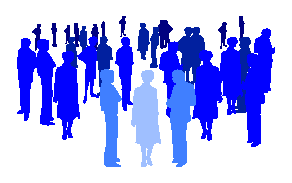
\includegraphics[scale=0.5]{img/estimacion/poblacion}}
\rput(10,7){Población}
\uncover<2->{
\psline{->}(4.5,6.2)(1.2,5.2)
\rput(1,5){$X_1$}
\rput(1,4){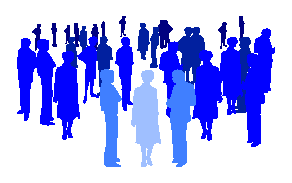
\includegraphics[scale=0.5]{img/estimacion/poblacion}}
\psline{->}(4.5,6.2)(4,5.2)
\rput(4,5){$X_2$}
\rput(4,4){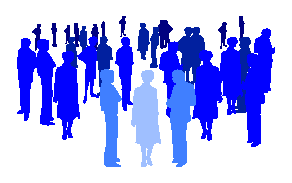
\includegraphics[scale=0.5]{img/estimacion/poblacion}}
\rput(6,4.2){$n$ copias}
\rput(6,4){$\ldots$}
\psline{->}(4.5,6.2)(7.8,5.2)
\rput(8,5){$X_n$}
\rput(8,4){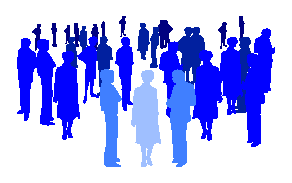
\includegraphics[scale=0.5]{img/estimacion/poblacion}}
\rput(10,5){Variable}
\rput(10,4.5){aleatoria}
\rput(10,4){muestral}
}
\uncover<3->{
\psline{->}(1,3)(1,2)
\rput(0.5,1){$x_1$}
\rput(1,1){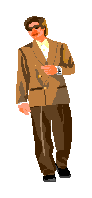
\includegraphics[scale=0.45]{img/estimacion/individuo1}}
\psline{->}(4,3)(4,2)
\rput(3.5,1){$x_2$}
\rput(4,1){
\includegraphics[scale=0.45]{img/estimacion/individuo2}}
\rput(6,1){$\ldots$}
\psline{->}(8,3)(8,2)
\rput(7.5,1){$x_n$}
\rput(8,1){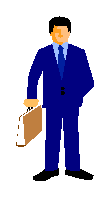
\includegraphics[scale=0.45]{img/estimacion/individuo3}}
\rput(10,1){Muestra}
}
\end{pspicture}
\end{center}
\end{frame}


%---------------------------------------------------------------------slide----
\begin{frame}
\frametitle{Estimación de parámetros}
Las tres cuestiones fundamentales respecto a la variable aleatoria muestral son:
\begin{description}
\item [Homogeneidad]: Las $n$ variables que componen la variable aleatoria muestral siguen la misma distribución.
\item [Independencia]: Las variables son independientes entre sí.
\item [Modelo de distribución]: El modelo de distribución que siguen las $n$ variables.
\end{description}
Las dos primeras cuestiones pueden resolverse si se utiliza muestreo aleatorio simple para obtener la muestra. En cuanto a la última, hay que responder, a su vez, a dos cuestiones:
\begin{itemize}
\item ¿Qué modelo de distribución se ajusta mejor a nuestro conjunto de datos? Esto se resolverá, en parte, mediante la utilización de técnicas no paramétricas.
\item Una vez seleccionado el modelo de distribución más apropiado, ¿qué estadístico del modelo nos interesa y cómo determinar su valor? 
De esto último se encarga la parte de la inferencia estadística conocida como \structure{\textbf{Estimación de Parámetros}}.
\end{itemize}
\end{frame}


%---------------------------------------------------------------------slide----
\begin{frame}
\frametitle{Parámetros a estimar}
En este tema se abordará la segunda cuestión, es decir, suponiendo que se conoce el modelo de distribución de una población, se intentará estimar los principales parámetros que la definen.
Por ejemplo, los principales parámetros que definen las distribuciones vistas en el tema anterior son:
\begin{center}
\begin{tabular}{|l|c|}
\hline
Distribución & Parámetro \\
\hline\hline
Binomial & $n,p$\\
\hline
Poisson & $\lambda$\\
\hline
Uniforme & $a,b$\\
\hline
Normal & $\mu,\sigma$\\
\hline
Chi-cuadrado & $n$\\
\hline
T-Student & $n$\\
\hline
F-Fisher & $m,n$\\
\hline
\end{tabular}
\end{center}
\end{frame}


%---------------------------------------------------------------------slide----
\begin{frame}
\frametitle{Distribución de la variable aleatoria muestral}
La distribución de probabilidad de los valores de la variable muestral depende claramente de la distribución de probabilidad de los valores de la población.

Ejemplo: Sea una población en la que la cuarta parte de las familias no tienen hijos, la mitad de las familias tiene 1 hijo, y el resto tiene 2 hijos.

\begin{center}
\tikzsetnextfilename{estimacion/distribucion_variable_muestral}
\begin{tikzpicture}
\matrix[column sep=2em, ampersand replacement=\&] {
\node{
$
\begin{array}{|c|c|}
\multicolumn{2}{c}{\mbox{Distribución}}\\
\multicolumn{2}{c}{\mbox{Poblacional}}\\
\hline
X & P(x)\\
\hline\hline
0 & 0.25 \\
\hline
1 & 0.50 \\
\hline
2 & 0.25 \\
\hline
\end{array}
$
};
\&
\node at (0,0) [fill=color1, single arrow, shape border rotate=0, text=white, minimum width=1.1cm, align=left]{Muestras de\\ tamaño 2};
\&
\node{
$
\begin{array}{|c|c|}
\multicolumn{2}{c}{\mbox{Distribución muestral}}\\
\hline
(X_1,X_2) & P(x_1,x_2)\\
\hline\hline
(0,0) & 0.0625 \\
\hline
(0,1) & 0.1250 \\
\hline
(0,2) & 0.0625 \\
\hline
(1,0) & 0.1250 \\
\hline
(1,1) & 0.2500 \\
\hline
(1,2) & 0.1250 \\
\hline
(2,0) & 0.0625 \\
\hline
(2,1) & 0.1250 \\
\hline
(2,2) & 0.0625 \\
\hline
\end{array}
$
}; 
\\
};
\end{tikzpicture}
\end{center}
\end{frame}


%---------------------------------------------------------------------slide----
\begin{frame}
\frametitle{Distribución de un estadístico muestral}
Por ser función de una variable aleatoria, un estadístico en el muestreo es también una variable aleatoria.
Por tanto, su distribución de probabilidad también depende de la distribución de la población y de los parámetros que la determinan ($\mu,\sigma,p,\ldots $).

Ejemplo: Si se toma la media muestral $\bar X$ de las muestras de tamaño 2 del ejemplo anterior, su distribución de probabilidad es
\begin{center}
\tikzsetnextfilename{estimacion/distribucion_media}
\begin{tikzpicture}
\matrix[column sep=2em, ampersand replacement=\&] {
\node{
$
\begin{array}{|c|c|}
\multicolumn{2}{c}{\mbox{Distribución muestral}}\\
\hline
(X_1,X_2) & P(x_1,x_2)\\
\hline\hline
(0,0) & 0.0625 \\
\hline
(0,1) & 0.1250 \\
\hline
(0,2) & 0.0625 \\
\hline
(1,0) & 0.1250 \\
\hline
(1,1) & 0.2500 \\
\hline
(1,2) & 0.1250 \\
\hline
(2,0) & 0.0625 \\
\hline
(2,1) & 0.1250 \\
\hline
(2,2) & 0.0625 \\
\hline
\end{array}
$
};
\&
\node at (0,0) [fill=color1, single arrow, shape border rotate=0, text=white, minimum width=1.1cm, align=left]{$\bar x=\frac{X_1+X_2}{2}$};
\&
\node{
$
\begin{array}{|c|c|}
\multicolumn{2}{c}{\mbox{Distribución}}\\
\multicolumn{2}{c}{\mbox{de $\bar{x}$}}\\
\hline
\bar X & P(x)\\
\hline\hline
0 & 0.0625 \\
\hline
0.5 & 0.2500 \\
\hline
1 & 0.3750 \\
\hline
1.5 & 0.2500\\
\hline
2 & 0.0625 \\
\hline
\end{array}
$
}; 
\\
};
\end{tikzpicture}
\end{center}
\end{frame}

%---------------------------------------------------------------------slide----
\begin{frame}
\frametitle{Distribución de un estadístico muestral}
\begin{center}
\tikzsetnextfilename{estimacion/diagrama_barras_distribucion_poblacion}
\resizebox{0.49\textwidth}{!}{\input{img/estimacion/diagrama_barras_distribucion_poblacion}}
\tikzsetnextfilename{estimacion/diagrama_barras_distribucion_media}
\resizebox{0.49\textwidth}{!}{\input{img/estimacion/diagrama_barras_distribucion_media}}

\emph{¿Cuál es la probabilidad de obtener una media muestral que aproxime la media poblacional con un error máximo de 0.5?}
\end{center}
\end{frame}


%---------------------------------------------------------------------slide----
\begin{frame}
\frametitle{Teorema central del límite}
Como hemos visto, para conocer la distribución de un estadístico muestral, es necesario conocer la distribución de la población, lo cual no siempre es posible. 
Afortunadamente, para muestras grandes es posible aproximar la distribución de algunos estadísticos como la media, gracias al siguiente teorema:

\begin{teorema}[Teorema central del límite]
Si $X_1,\ldots, X_n$ son variables aleatorias independientes  ($n\geq 30$) con medias y varianzas $\mu_i=E(X_i)$, $\sigma^2_i=Var(X_i)$, $i=1,\ldots,n$ respectivamente, entonces la variable aleatoria $X=X_1+\cdots+X_n$ sigue una distribución aproximadamente normal de media la suma de las medias y varianza la suma de las varianzas
\[
X=X_1+\cdots+X_n\stackrel{n\geq 30} \sim N\left(\sum_{i=1}^n \mu_i, \sqrt{\sum_{i=1}^n \sigma^2_i}\right)
\]
\end{teorema}

Este teorema además es la explicación de que la mayoría de las variables biológicas presenten una distribución normal, ya que suelen ser causa de múltiples factores que suman sus efectos de manera independiente.
\end{frame}


%---------------------------------------------------------------------slide----
\begin{frame}
\frametitle{Distribución de la media muestral}
\framesubtitle{Muestras grandes ($n\geq 30$)}
La media muestral de una muestra aleatoria de tamaño $n$ es la suma de $n$ variables aleatorias independientes, idénticamente distribuidas:
\[
\bar X = \frac{X_1+\cdots+X_n}{n} = \frac{X_1}{n}+\cdots+\frac{X_n}{n}
\]
De acuerdo a las propiedades de las transformaciones lineales, la media y la varianza de cada una de estas variables son
\[
E\left(\frac{X_i}{n}\right) =\frac{\mu}{n} \quad  \mbox{y} \quad Var\left(\frac{X_i}{n}\right) = \frac{\sigma^2}{n^2}
\]
con $\mu$ y $\sigma^2$ la media y la varianza de la población de partida.

Entonces, si el tamaño de la muestra es grande ($n\geq 30$), de acuerdo al teorema central del límite, la distribución de la media muestral será normal:
\[
\bar X \sim N\left(\sum_{i=1}^n \frac{\mu}{n},\sqrt{\sum_{i=1}^n \frac{\sigma^2}{n^2}} \right) = N\left(\mu,\frac{\sigma}{\sqrt{n}} \right).
\]
\end{frame}


%---------------------------------------------------------------------slide----
\begin{frame}
\frametitle{Distribución de la media muestral}
\framesubtitle{Ejemplo para muestras grandes ($n\geq 30$)}
Supongase que se desea estimar el número medio de hijos de una población con media $\mu=2$ hijos y desviación típica $\sigma=1$ hijo.
\begin{center}
\emph{¿Qué probabilidad hay de estimar $\mu$ a partir de $\bar x$ con un error menor de $0.2$?}
\end{center}
\begin{columns}
\begin{column}{0.5\textwidth}
De acuerdo al teorema central del límite se tiene:
\begin{itemize}
\item Para $n=30$, $\bar x\sim N(2,1/\sqrt{30})$ y
\[
P(1.8<\bar x<2.2) = 0.7267.
\]

\item Para $n=100$, $\bar x\sim N(2,1/\sqrt{100})$ y
\[
P(1.8<\bar x<2.2) = 0.9545.
\]
\end{itemize}
\end{column}
\begin{column}{0.5\textwidth}
\begin{center}
\tikzsetnextfilename{estimacion/teorema_central_limite}
\scalebox{0.7}{%% Input file name: estimacion/teorema_central_limite.fig
%% FIG version: 3.2
%% Orientation: Landscape
%% Justification: Flush Left
%% Units: Inches
%% Paper size: A4
%% Magnification: 100.0
%% Resolution: 1200ppi

\begin{pspicture}(6.68cm,3.48cm)(16.72cm,13.45cm)
\psset{unit=0.8cm}
%%
%% Depth: 2147483647
%%
\newrgbcolor{mycolor0}{1.00 0.50 0.31}\definecolor{mycolor0}{rgb}{1.00,0.50,0.31}
\newgray{mycolor2}{0.74}\definecolor{mycolor2}{gray}{0.74}
%%
%% Depth: 100
%%
\psset{linestyle=solid,linewidth=0.03175,linecolor=mycolor0,fillstyle=none}
\psline(10.61,6.80)(10.67,6.80)(10.73,6.80)(10.79,6.80)(10.86,6.80)(10.92,6.80)(10.98,6.80)(11.05,6.80)(11.11,6.80)(11.17,6.80)(11.23,6.80)(11.30,6.80)(11.36,6.80)(11.42,6.80)(11.49,6.80)(11.55,6.80)(11.61,6.80)(11.67,6.80)(11.73,6.80)(11.80,6.80)(11.86,6.80)(11.92,6.80)(11.98,6.80)(12.05,6.80)(12.11,6.80)(12.17,6.80)(12.24,6.80)(12.30,6.80)(12.36,6.80)(12.42,6.80)(12.49,6.80)(12.55,6.80)(12.61,6.80)(12.67,6.80)(12.74,6.80)(12.80,6.80)(12.86,6.80)(12.92,6.80)(12.99,6.80)(13.05,6.80)(13.11,6.80)(13.17,6.80)(13.24,6.80)(13.30,6.80)(13.36,6.80)(13.43,6.80)(13.49,6.81)(13.55,6.81)(13.61,6.81)(13.68,6.82)(13.74,6.84)(13.80,6.86)(13.86,6.89)(13.93,6.93)(13.99,6.99)(14.05,7.07)(14.11,7.17)(14.18,7.32)(14.24,7.50)(14.30,7.74)(14.36,8.03)(14.43,8.38)(14.49,8.80)(14.55,9.28)(14.62,9.83)(14.68,10.42)(14.74,11.06)(14.80,11.72)(14.87,12.38)(14.93,13.02)(14.99,13.61)(15.05,14.12)(15.12,14.52)(15.18,14.81)(15.24,14.95)(15.30,14.95)(15.37,14.81)(15.43,14.52)(15.49,14.12)(15.56,13.61)(15.62,13.02)(15.68,12.38)(15.74,11.72)(15.81,11.06)(15.87,10.42)(15.93,9.83)(15.99,9.28)(16.05,8.80)(16.12,8.38)(16.18,8.03)(16.24,7.74)(16.30,7.50)(16.37,7.32)(16.43,7.17)(16.49,7.07)(16.56,6.99)(16.62,6.93)(16.68,6.89)(16.74,6.86)(16.81,6.84)(16.87,6.82)(16.93,6.81)(16.99,6.81)(17.06,6.81)(17.12,6.80)(17.18,6.80)(17.24,6.80)(17.31,6.80)(17.37,6.80)(17.43,6.80)(17.50,6.80)(17.56,6.80)(17.62,6.80)(17.68,6.80)(17.75,6.80)(17.81,6.80)(17.87,6.80)(17.93,6.80)(18.00,6.80)(18.06,6.80)(18.12,6.80)(18.18,6.80)(18.25,6.80)(18.31,6.80)(18.37,6.80)(18.43,6.80)(18.50,6.80)(18.56,6.80)(18.62,6.80)(18.69,6.80)(18.75,6.80)(18.81,6.80)(18.87,6.80)(18.94,6.80)(19.00,6.80)(19.06,6.80)(19.12,6.80)(19.19,6.80)(19.25,6.80)(19.31,6.80)(19.37,6.80)(19.44,6.80)(19.50,6.80)(19.56,6.80)(19.62,6.80)(19.69,6.80)(19.75,6.80)(19.81,6.80)(19.88,6.80)(19.94,6.80)
\psset{linecolor=black}
\psline(10.61,6.47)(19.94,6.47)
\psline(10.61,6.47)(10.61,6.26)
\psline(12.94,6.47)(12.94,6.26)
\psline(15.27,6.47)(15.27,6.26)
\psline(17.60,6.47)(17.60,6.26)
\psline(19.94,6.47)(19.94,6.26)
\rput(10.61,5.71){1.0}
\rput(12.94,5.71){1.5}
\rput(15.27,5.71){2.0}
\rput(17.60,5.71){2.5}
\rput(19.94,5.71){3.0}
\psline(10.23,6.80)(10.23,14.99)
\psline(10.23,6.80)(10.02,6.80)
\psline(10.23,8.85)(10.02,8.85)
\psline(10.23,10.90)(10.02,10.90)
\psline(10.23,12.94)(10.02,12.94)
\psline(10.23,14.99)(10.02,14.99)
\rput{90}(9.73,6.80){0}
\rput{90}(9.73,8.85){1}
\rput{90}(9.73,10.90){2}
\rput{90}(9.73,12.94){3}
\rput{90}(9.73,14.99){4}
\psline(10.23,6.47)(20.31,6.47)(20.31,15.28)(10.23,15.28)(10.23,6.47)
\rput[c](15.27,16.25){Distribuciones de la media muestral del nº de hijos}
\rput[c](15.27,15.75){Población con $\mu=2$ hijos y $\sigma=1$ hijo}
\rput(15.27,4.86){$\bar x$}
\rput[c]{90}(8.86,10.90){$f(x)$}
\psset{linecolor=green}
\psline(10.61,6.80)(10.67,6.80)(10.73,6.80)(10.79,6.80)(10.86,6.80)(10.92,6.80)(10.98,6.80)(11.05,6.80)(11.11,6.80)(11.17,6.80)(11.23,6.80)(11.30,6.80)(11.36,6.80)(11.42,6.80)(11.49,6.80)(11.55,6.80)(11.61,6.80)(11.67,6.80)(11.73,6.80)(11.80,6.80)(11.86,6.80)(11.92,6.80)(11.98,6.80)(12.05,6.80)(12.11,6.80)(12.17,6.81)(12.24,6.81)(12.30,6.81)(12.36,6.81)(12.42,6.82)(12.49,6.82)(12.55,6.83)(12.61,6.83)(12.67,6.84)(12.74,6.85)(12.80,6.86)(12.86,6.88)(12.92,6.90)(12.99,6.92)(13.05,6.95)(13.11,6.98)(13.17,7.01)(13.24,7.06)(13.30,7.11)(13.36,7.16)(13.43,7.23)(13.49,7.30)(13.55,7.38)(13.61,7.47)(13.68,7.57)(13.74,7.68)(13.80,7.81)(13.86,7.94)(13.93,8.08)(13.99,8.24)(14.05,8.40)(14.11,8.57)(14.18,8.75)(14.24,8.94)(14.30,9.14)(14.36,9.33)(14.43,9.53)(14.49,9.73)(14.55,9.93)(14.62,10.12)(14.68,10.31)(14.74,10.48)(14.80,10.64)(14.87,10.79)(14.93,10.92)(14.99,11.04)(15.05,11.13)(15.12,11.20)(15.18,11.25)(15.24,11.27)(15.30,11.27)(15.37,11.25)(15.43,11.20)(15.49,11.13)(15.56,11.04)(15.62,10.92)(15.68,10.79)(15.74,10.64)(15.81,10.48)(15.87,10.31)(15.93,10.12)(15.99,9.93)(16.05,9.73)(16.12,9.53)(16.18,9.33)(16.24,9.14)(16.30,8.94)(16.37,8.75)(16.43,8.57)(16.49,8.40)(16.56,8.24)(16.62,8.08)(16.68,7.94)(16.74,7.81)(16.81,7.68)(16.87,7.57)(16.93,7.47)(16.99,7.38)(17.06,7.30)(17.12,7.23)(17.18,7.16)(17.24,7.11)(17.31,7.06)(17.37,7.01)(17.43,6.98)(17.50,6.95)(17.56,6.92)(17.62,6.90)(17.68,6.88)(17.75,6.86)(17.81,6.85)(17.87,6.84)(17.93,6.83)(18.00,6.83)(18.06,6.82)(18.12,6.82)(18.18,6.81)(18.25,6.81)(18.31,6.81)(18.37,6.81)(18.43,6.80)(18.50,6.80)(18.56,6.80)(18.62,6.80)(18.69,6.80)(18.75,6.80)(18.81,6.80)(18.87,6.80)(18.94,6.80)(19.00,6.80)(19.06,6.80)(19.12,6.80)(19.19,6.80)(19.25,6.80)(19.31,6.80)(19.37,6.80)(19.44,6.80)(19.50,6.80)(19.56,6.80)(19.62,6.80)(19.69,6.80)(19.75,6.80)(19.81,6.80)(19.88,6.80)(19.94,6.80)
\psset{linecolor=mycolor2}
\psline(10.23,6.80)(20.31,6.80)
\psset{linecolor=black}
\psline(10.23,6.47)(10.23,6.47)
\psset{linecolor=green}
\psline(18.20,14.57)(18.90,14.57)
\rput[l](19,14.57){n=30}
\psset{linecolor=mycolor0}
\psline(18.20,14.15)(18.90,14.15)
\rput[l](19,14.15){n=100}
\end{pspicture}
%% End
}
\end{center}
\end{column}
\end{columns}
\end{frame}


%---------------------------------------------------------------------slide----
\begin{frame}
\frametitle{Distribución de una proporción muestral}
\framesubtitle{Muestras grandes ($n\geq 30$)}
Una proporción $p$ poblacional puede calcularse como la media de una variable dicotómica (0,1).
Esta variable se conoce como \emph{variable de Bernouilli} $B(p)$, que es un caso particular de la binomial para $n=1$.
Por tanto, para una muestra aleatoria de tamaño $n$, una proporción muestral $\hat p$ también puede expresarse como la suma de $n$ variables aleatorias independientes, idénticamente distribuidas:
\[
\hat p = \bar X = \frac{X_1+\cdots+X_n}{n} = \frac{X_1}{n}+\cdots+\frac{X_n}{n}, \mbox{ con } X_i\sim B(p)
\]
y con media y varianza
\[
E\left(\frac{X_i}{n}\right) =\frac{p}{n} \quad  \mbox{y} \quad Var\left(\frac{X_i}{n}\right) = \frac{p(1-p)}{n^2}
\]

Entonces, si el tamaño de la muestra es grande ($n\geq 30$), de acuerdo al teorema central del límite, la distribución de la proporción muestral también será normal:
\[
\hat p \sim N\left(\sum_{i=1}^n \frac{p}{n},\sqrt{\sum_{i=1}^n \frac{p(1-p)}{n^2}} \right) = N\left(p,\sqrt{\frac{p(1-p)}{n}} \right).
\]
\end{frame}


\subsection{Estimadores}
%---------------------------------------------------------------------slide----
\begin{frame}
\frametitle{Estimador y estimación}
Los estadísticos muestrales pueden utilizarse para aproximar los parámetros de la población, y cuando un estadístico se utiliza con este fin se le llama \emph{estimador del parámetro}.
\begin{definicion}[Estimador y estimación]
Un \emph{estimador} es una función de la variable aleatoria muestral
\[
\hat \theta = F(X_1,\ldots,X_n).
\]
Dada una muestra concreta $(x_1,\ldots,x_n)$, el valor del estimador aplicado a ella se conoce como \emph{estimación}
\[
\hat \theta_0 = F(x_1,\ldots,x_n).
\]
\end{definicion}

Por ser una función de la variable aleatoria muestral, un estimador es, a su vez, una variable aleatoria cuya distribución depende de la población de partida.

Mientras que el estimador es una función que es única, la estimación no es única, sino que depende de la muestra tomada.
\end{frame}


%---------------------------------------------------------------------slide----
\begin{frame}
\frametitle{Estimador y estimación}
\begin{center}
\tikzsetnextfilename{estimacion/estimador_estimacion}
\begin{pspicture}(0,0)(11,8)
\rput(2,7){Distribución de la población}
\rput(2,6.5){$X$}
\uncover<2->{
\psline[linewidth=10pt,linecolor=royalblue1,arrowlength=1,arrowinset=0]{->}(4.5,6.5)(5.5,6.5)
\rput(5,6.5){?}
\rput(8,7){Parámetro poblacional}
\rput(8,6.5){$\theta$}
}
\uncover<3->{
\psline[linewidth=10pt,linecolor=royalblue1,arrowlength=1,arrowinset=0]{->}(2,6)(2,5)
\rput(2,4.5){Variable aleatoria muestral}
\rput(2,4){$(X_1,\ldots,X_n)$}
}
\uncover<4->{
\psline[linewidth=10pt,linecolor=royalblue1,arrowlength=1,arrowinset=0]{->}(4.5,4)(5.5,4)
\rput(8,4.5){Estimador}
\rput(8,4){$\hat \theta = F(X_1,\ldots,X_n)$}
}
\uncover<5->{
\psline[linewidth=10pt,linecolor=royalblue1,arrowlength=1,arrowinset=0]{->}(2,3.5)(2,2.5)
\rput(2,2){Muestra de tamaño $n$}
\rput(2,1.5){$(x_1,\ldots,x_n)$}
}
\uncover<6->{
\psline[linewidth=10pt,linecolor=royalblue1,arrowlength=1,arrowinset=0]{->}(4.5,1.5)(5.5,1.5)
\rput(8,2){Estimación}
\rput(8,1.5){$\hat \theta_0 = F(x_1,\ldots,x_n)$}
}
\uncover<7->{
\pscurve[linewidth=5pt,linecolor=royalblue1,arrowlength=1,arrowinset=0]{->}(9.5,1.7)(10,4)(9.5,6.3)
}
\end{pspicture}
\end{center}
\end{frame}


%---------------------------------------------------------------------slide----
\begin{frame}
\frametitle{Estimador y estimación}
\framesubtitle{Ejemplo}
Supóngase que se quiere saber la proporción $p$ de fumadores en una ciudad.
En ese caso, la variable dicotómica que mide si una persona fuma (1) o no (0), sigue una distribución de Bernouilli $B(p)$.

Si se toma una muestra aleatoria de tamaño 5, $(X_1,X_2,X_3,X_4,X_5)$, de esta población, se puede utilizar la proporción de fumadores en la muestra como estimador para la proporción de fumadores en la población:
\[
\hat p = \frac{\sum_{i=1}^5 X_i}{5}
\]
Este estimador es una variable que se distribuye
$\hat p\sim \frac{1}{n}B\left(p,\sqrt{\frac{p(1-p)}{n}}\right)$.

Si se toman distintas muestras, se obtienen diferentes estimaciones:
\[
\begin{array}{|c|c|}
\hline
\mbox{Muestra} & \mbox{Estimación}\\
\hline\hline
(1, 0, 0, 1, 1) & 3/5\\
\hline
(1, 0, 0, 0, 0) & 1/5\\
\hline
(0, 1, 0, 0, 1) & 2/5\\
\hline
\cdots & \cdots\\
\hline
\end{array}
\]
\end{frame}


%---------------------------------------------------------------------slide----
\begin{frame}
\frametitle{Tipos de estimación}
La estimación de parámetros puede realizar de de dos formas:
\begin{description}
\item[Estimación puntual]: Se utiliza un único estimador que proporciona un valor o estimación aproximada del parámetro.
El principal inconveniente de este tipo de estimación es que no se especifica la bondad de la estimación.
\item[Estimación por intervalos]: Se utilizan dos estimadores que proporcionan los extremos de un intervalo dentro del cual se cree que está el verdadero valor del parámetro con un cierto grado de seguridad.
Esta forma de estimar sí permite controlar el error cometido en la estimación.
\end{description}

\begin{center}
\tikzsetnextfilename{estimacion/estimacion_puntual_intervalo}
\begin{tikzpicture}
\node at (1.5,1) {Estimación puntual};
\draw (0,0.5) -- (3,0.5);
\draw (1.5,0.6) -- (1.5,0.4);
\node at (1.5,0) {$\theta$};
\draw[color=color2] (2,0.6) -- (2,0.4);
\node[color=color2] at (2,0) {$\hat\theta_0$};
\node at (7.5,1) {Estimación por intervalo};
\draw (6,0.5) -- (9,0.5);
\draw (7.5,0.6) -- (7.5,0.4);
\node at (7.5,0) {$\theta$};
\node[color=color2] at (7,0.5) {[};
\node[color=color2] at (8.2,0.5) {]};
\node[color=color2] at (7,0) {$l_1$};
\node[color=color2] at (8.2,0) {$l_2$};
\end{tikzpicture}
\end{center}
\end{frame}


\subsection{Estimación puntual}
%---------------------------------------------------------------------slide----
\begin{frame}
\frametitle{Estimación puntual}
La estimación puntual utiliza un único estimador para estimar el valor del parámetro desconocido de la población.

En teoría pueden utilizarse distintos estimadores para estimar un mismo parámetro. Por ejemplo, en el caso de estimar la proporción de fumadores en una ciudad, podrían haberse utilizado otros posibles estimadores además de la proporción muestral, como pueden ser:
\begin{align*}
\hat \theta_1 &= \sqrt[5]{X_1X_2X_3X_4X_5}\\
\hat \theta_2 &= \frac{X_1+X_5}{2}\\
\hat \theta_3 &= X_1 \cdots
\end{align*}

\begin{center}
\alert{\emph{¿Cuál es el mejor estimador?}}
\end{center}

La respuesta a esta cuestión depende de las propiedades de cada estimador.
\end{frame}


%---------------------------------------------------------------------slide----
\begin{frame}
\frametitle{Propiedades de los estimadores}
Aunque la estimación puntual no proporciona ninguna medida del grado de bondad de la estimación, existen varias propiedades que garantizan dicha bondad.

Las propiedades más deseables en un estimador son:
\begin{itemize}
\item Insesgadez
\item Eficiencia
\item Consistencia
\item Normalidad asintótica
\item Suficiencia
\end{itemize}
\end{frame}


%---------------------------------------------------------------------slide----
\begin{frame}
\frametitle{Insesgadez}
\begin{definicion}[Estimador insesgado]
Un estimador $\hat \theta$ es \emph{insesgado} para un parámetro $\theta$ si su esperanza es precisamente $\theta$, es decir,
\[
E(\hat \theta)=\theta.
\]
\end{definicion}
\begin{center}
\tikzsetnextfilename{estimacion/estimadores_sesgados_insesgados}
\scalebox{0.7}{%% Input file name: estimacion/estimadores_sesgados_insesgados.fig
%% FIG version: 3.2
%% Orientation: Landscape
%% Justification: Flush Left
%% Units: Inches
%% Paper size: Letter
%% Magnification: 100.0
%% Resolution: 1200ppi

\begin{pspicture}(5.97cm,3.71cm)(16.34cm,13.69cm)
\psset{unit=0.8cm}
%%
%% Depth: 2147483647
%%
\newrgbcolor{mycolor0}{1.00 0.50 0.31}\definecolor{mycolor0}{rgb}{1.00,0.50,0.31}
\newrgbcolor{mycolor2}{0.28 0.46 1.00}\definecolor{mycolor2}{rgb}{0.28,0.46,1.00}
\newgray{mycolor3}{0.74}\definecolor{mycolor3}{gray}{0.74}
%%
%% Depth: 100
%%
\psset{linestyle=solid,linewidth=0.03175,linecolor=mycolor0,fillstyle=none}
\psline(10.56,7.09)(10.63,7.10)(10.71,7.11)(10.79,7.12)(10.86,7.14)(10.94,7.16)(11.02,7.18)(11.10,7.21)(11.18,7.24)(11.25,7.27)(11.33,7.32)(11.41,7.37)(11.49,7.42)(11.56,7.49)(11.64,7.56)(11.72,7.65)(11.80,7.74)(11.87,7.85)(11.95,7.97)(12.03,8.10)(12.11,8.25)(12.18,8.42)(12.26,8.60)(12.34,8.79)(12.42,9.00)(12.49,9.23)(12.57,9.47)(12.65,9.73)(12.73,10.01)(12.80,10.29)(12.88,10.59)(12.96,10.90)(13.04,11.22)(13.11,11.54)(13.19,11.87)(13.27,12.20)(13.35,12.53)(13.42,12.86)(13.50,13.17)(13.58,13.48)(13.66,13.77)(13.73,14.04)(13.81,14.29)(13.89,14.52)(13.97,14.72)(14.04,14.89)(14.12,15.03)(14.20,15.14)(14.28,15.21)(14.35,15.25)(14.43,15.25)(14.51,15.21)(14.59,15.14)(14.66,15.03)(14.74,14.89)(14.82,14.72)(14.90,14.52)(14.97,14.29)(15.05,14.04)(15.13,13.77)(15.21,13.48)(15.28,13.17)(15.36,12.86)(15.44,12.53)(15.52,12.20)(15.59,11.87)(15.67,11.54)(15.75,11.22)(15.83,10.90)(15.90,10.59)(15.98,10.29)(16.06,10.01)(16.14,9.73)(16.21,9.47)(16.29,9.23)(16.37,9.00)(16.45,8.79)(16.52,8.60)(16.60,8.42)(16.68,8.25)(16.76,8.10)(16.83,7.97)(16.91,7.85)(16.99,7.74)(17.07,7.65)(17.14,7.56)(17.22,7.49)(17.30,7.42)(17.38,7.37)(17.45,7.32)(17.53,7.27)(17.61,7.24)(17.69,7.21)(17.77,7.18)(17.84,7.16)(17.92,7.14)(18.00,7.12)(18.08,7.11)(18.15,7.10)(18.23,7.09)
\psset{linecolor=black}
\psline(9.36,7.05)(9.36,15.27)
\psline(9.36,7.05)(9.14,7.05)
\psline(9.36,9.11)(9.14,9.11)
\psline(9.36,11.16)(9.14,11.16)
\psline(9.36,13.22)(9.14,13.22)
\psline(9.36,15.27)(9.14,15.27)
\rput[B]{90}(8.85,7.05){0.0}
\rput[B]{90}(8.85,9.11){0.1}
\rput[B]{90}(8.85,11.16){0.2}
\rput[B]{90}(8.85,13.22){0.3}
\rput[B]{90}(8.85,15.27){0.4}
\psline(9.36,6.77)(19.43,6.77)(19.43,15.57)(9.36,15.57)(9.36,6.77)
\rput[B](14.39,16.29){Distribuciones de estimadores sesgados e insesgados}
\rput[B](14.39,5.16){Valores de los estimadores}
\rput[lB]{90}(7.98,9.84){Densidad $f(x)$}
\psset{linestyle=dashed,linecolor=green}
\psline(9.39,7.09)(9.47,7.10)(9.54,7.11)(9.62,7.12)(9.70,7.14)(9.78,7.16)(9.85,7.18)(9.93,7.21)(10.01,7.24)(10.09,7.27)(10.16,7.32)(10.24,7.37)(10.32,7.42)(10.40,7.49)(10.47,7.56)(10.55,7.65)(10.63,7.74)(10.71,7.85)(10.78,7.97)(10.86,8.10)(10.94,8.25)(11.02,8.42)(11.09,8.60)(11.17,8.79)(11.25,9.00)(11.33,9.23)(11.40,9.47)(11.48,9.73)(11.56,10.01)(11.64,10.29)(11.71,10.59)(11.79,10.90)(11.87,11.22)(11.95,11.54)(12.02,11.87)(12.10,12.20)(12.18,12.53)(12.26,12.86)(12.33,13.17)(12.41,13.48)(12.49,13.77)(12.57,14.04)(12.64,14.29)(12.72,14.52)(12.80,14.72)(12.88,14.89)(12.95,15.03)(13.03,15.14)(13.11,15.21)(13.19,15.25)(13.27,15.25)(13.34,15.21)(13.42,15.14)(13.50,15.03)(13.58,14.89)(13.65,14.72)(13.73,14.52)(13.81,14.29)(13.89,14.04)(13.96,13.77)(14.04,13.48)(14.12,13.17)(14.20,12.86)(14.27,12.53)(14.35,12.20)(14.43,11.87)(14.51,11.54)(14.58,11.22)(14.66,10.90)(14.74,10.59)(14.82,10.29)(14.89,10.01)(14.97,9.73)(15.05,9.47)(15.13,9.23)(15.20,9.00)(15.28,8.79)(15.36,8.60)(15.44,8.42)(15.51,8.25)(15.59,8.10)(15.67,7.97)(15.75,7.85)(15.82,7.74)(15.90,7.65)(15.98,7.56)(16.06,7.49)(16.13,7.42)(16.21,7.37)(16.29,7.32)(16.37,7.27)(16.44,7.24)(16.52,7.21)(16.60,7.18)(16.68,7.16)(16.75,7.14)(16.83,7.12)(16.91,7.11)(16.99,7.10)(17.06,7.09)
\psset{linecolor=mycolor2}
\psline(11.72,7.09)(11.80,7.10)(11.88,7.11)(11.95,7.12)(12.03,7.14)(12.11,7.16)(12.19,7.18)(12.26,7.21)(12.34,7.24)(12.42,7.27)(12.50,7.32)(12.57,7.37)(12.65,7.42)(12.73,7.49)(12.81,7.56)(12.88,7.65)(12.96,7.74)(13.04,7.85)(13.12,7.97)(13.19,8.10)(13.27,8.25)(13.35,8.42)(13.43,8.60)(13.50,8.79)(13.58,9.00)(13.66,9.23)(13.74,9.47)(13.81,9.73)(13.89,10.01)(13.97,10.29)(14.05,10.59)(14.12,10.90)(14.20,11.22)(14.28,11.54)(14.36,11.87)(14.43,12.20)(14.51,12.53)(14.59,12.86)(14.67,13.17)(14.74,13.48)(14.82,13.77)(14.90,14.04)(14.98,14.29)(15.05,14.52)(15.13,14.72)(15.21,14.89)(15.29,15.03)(15.36,15.14)(15.44,15.21)(15.52,15.25)(15.60,15.25)(15.68,15.21)(15.75,15.14)(15.83,15.03)(15.91,14.89)(15.99,14.72)(16.06,14.52)(16.14,14.29)(16.22,14.04)(16.30,13.77)(16.37,13.48)(16.45,13.17)(16.53,12.86)(16.61,12.53)(16.68,12.20)(16.76,11.87)(16.84,11.54)(16.92,11.22)(16.99,10.90)(17.07,10.59)(17.15,10.29)(17.23,10.01)(17.30,9.73)(17.38,9.47)(17.46,9.23)(17.54,9.00)(17.61,8.79)(17.69,8.60)(17.77,8.42)(17.85,8.25)(17.92,8.10)(18.00,7.97)(18.08,7.85)(18.16,7.74)(18.23,7.65)(18.31,7.56)(18.39,7.49)(18.47,7.42)(18.54,7.37)(18.62,7.32)(18.70,7.27)(18.78,7.24)(18.85,7.21)(18.93,7.18)(19.01,7.16)(19.09,7.14)(19.16,7.12)(19.24,7.11)(19.32,7.10)(19.40,7.09)
\psset{linestyle=solid,linecolor=mycolor3}
\psline(14.39,6.77)(14.39,15.57)
\psline(13.23,6.77)(13.23,15.57)
\psline(15.56,6.77)(15.56,15.57)
\psline(9.36,7.05)(19.43,7.05)
\psset{linecolor=black}
\psline(14.39,6.77)(14.39,6.77)
\psline(14.39,6.77)(14.39,6.56)
\rput[lB](14.28,5.93){$\theta$}
\psset{linecolor=mycolor0}
\psline(16.46,14.85)(17.09,14.85)
\rput[l](17.41,14.85){\scriptsize Insesgado}
\psset{linestyle=dashed,linecolor=green}
\psline(16.46,14.43)(17.09,14.43)
\rput[l](17.41,14.43){\scriptsize Sesgo -}
\psset{linecolor=mycolor2}
\psline(16.46,14.00)(17.09,14.00)
\rput[l](17.41,14){\scriptsize Sesgo +}
\end{pspicture}
%% End
}
\end{center}
\end{frame}


%---------------------------------------------------------------------slide----
\begin{frame}
\frametitle{Sesgo de un estimador}
Cuando un estimador no es insesgado, a la diferencia entre su esperanza y el valor del parámetro $\theta$ se le llama \emph{sesgo}:
\[
Sesgo(\hat \theta) = E(\hat \theta)-\theta.
\]

Cuanto menor sea el sesgo de un estimador, mejor se aproximarán sus estimaciones al verdadero valor del parámetro.
\end{frame}


%---------------------------------------------------------------------slide----
\begin{frame}
\frametitle{Consistencia}
\begin{definicion}[Estimador consistente]
Un estimador $\hat \theta_n$ para muestras de tamaño $n$ es \emph{consistente} para un parámetro $\theta$ si para cualquier valor $\epsilon>0$ se cumple
\[
\lim_{n\rightarrow \infty} P(|\hat \theta_n-\theta|<\epsilon)=1.
\]
\end{definicion}
\begin{center}
\tikzsetnextfilename{estimacion/estimadores_consistentes}
\resizebox{0.49\textwidth}{!}{% Created by tikzDevice version 0.10.1 on 2017-09-05 17:48:15
% !TEX encoding = UTF-8 Unicode
\begin{tikzpicture}[x=1pt,y=1pt]
\definecolor{fillColor}{RGB}{255,255,255}
\path[use as bounding box,fill=fillColor,fill opacity=0.00] (0,0) rectangle (325.21,238.49);
\begin{scope}
\path[clip] ( 49.20, 61.20) rectangle (300.01,189.29);
\definecolor{drawColor}{RGB}{0,0,0}

\path[draw=drawColor,line width= 0.4pt,line join=round,line cap=round] ( 58.49, 61.20) --
	( 60.16, 61.26) --
	( 61.83, 61.32) --
	( 63.50, 61.40) --
	( 65.17, 61.49) --
	( 66.84, 61.60) --
	( 68.51, 61.72) --
	( 70.18, 61.86) --
	( 71.86, 62.02) --
	( 73.53, 62.20) --
	( 75.20, 62.41) --
	( 76.87, 62.65) --
	( 78.54, 62.93) --
	( 80.21, 63.24) --
	( 81.88, 63.59) --
	( 83.55, 63.99) --
	( 85.22, 64.44) --
	( 86.89, 64.94) --
	( 88.56, 65.50) --
	( 90.23, 66.13) --
	( 91.90, 66.83) --
	( 93.58, 67.60) --
	( 95.25, 68.46) --
	( 96.92, 69.41) --
	( 98.59, 70.44) --
	(100.26, 71.58) --
	(101.93, 72.83) --
	(103.60, 74.19) --
	(105.27, 75.66) --
	(106.94, 77.26) --
	(108.61, 78.98) --
	(110.28, 80.84) --
	(111.95, 82.83) --
	(113.62, 84.97) --
	(115.30, 87.24) --
	(116.97, 89.65) --
	(118.64, 92.21) --
	(120.31, 94.92) --
	(121.98, 97.76) --
	(123.65,100.74) --
	(125.32,103.85) --
	(126.99,107.09) --
	(128.66,110.45) --
	(130.33,113.93) --
	(132.00,117.50) --
	(133.67,121.17) --
	(135.34,124.91) --
	(137.02,128.72) --
	(138.69,132.57) --
	(140.36,136.45) --
	(142.03,140.35) --
	(143.70,144.23) --
	(145.37,148.09) --
	(147.04,151.90) --
	(148.71,155.63) --
	(150.38,159.28) --
	(152.05,162.81) --
	(153.72,166.20) --
	(155.39,169.44) --
	(157.06,172.49) --
	(158.74,175.34) --
	(160.41,177.98) --
	(162.08,180.37) --
	(163.75,182.51) --
	(165.42,184.38) --
	(167.09,185.96) --
	(168.76,187.25) --
	(170.43,188.24) --
	(172.10,188.91) --
	(173.77,189.26) --
	(175.44,189.29) --
	(177.11,189.00) --
	(178.78,188.40) --
	(180.46,187.47) --
	(182.13,186.25) --
	(183.80,184.72) --
	(185.47,182.91) --
	(187.14,180.82) --
	(188.81,178.48) --
	(190.48,175.89) --
	(192.15,173.08) --
	(193.82,170.06) --
	(195.49,166.86) --
	(197.16,163.50) --
	(198.83,159.99) --
	(200.50,156.37) --
	(202.18,152.65) --
	(203.85,148.86) --
	(205.52,145.01) --
	(207.19,141.12) --
	(208.86,137.23) --
	(210.53,133.34) --
	(212.20,129.48) --
	(213.87,125.67) --
	(215.54,121.91) --
	(217.21,118.23) --
	(218.88,114.64) --
	(220.55,111.14) --
	(222.22,107.76) --
	(223.90,104.49) --
	(225.57,101.35) --
	(227.24, 98.34) --
	(228.91, 95.47) --
	(230.58, 92.74) --
	(232.25, 90.15) --
	(233.92, 87.71) --
	(235.59, 85.41) --
	(237.26, 83.25) --
	(238.93, 81.23) --
	(240.60, 79.34) --
	(242.27, 77.59) --
	(243.94, 75.97) --
	(245.61, 74.47) --
	(247.29, 73.09) --
	(248.96, 71.82) --
	(250.63, 70.66) --
	(252.30, 69.61) --
	(253.97, 68.64) --
	(255.64, 67.77) --
	(257.31, 66.98) --
	(258.98, 66.26) --
	(260.65, 65.62) --
	(262.32, 65.05) --
	(263.99, 64.53) --
	(265.66, 64.08) --
	(267.33, 63.67) --
	(269.01, 63.31) --
	(270.68, 62.99) --
	(272.35, 62.71) --
	(274.02, 62.46) --
	(275.69, 62.24) --
	(277.36, 62.05) --
	(279.03, 61.89) --
	(280.70, 61.74) --
	(282.37, 61.62) --
	(284.04, 61.51) --
	(285.71, 61.42) --
	(287.38, 61.34) --
	(289.05, 61.27) --
	(290.73, 61.21);
\end{scope}
\begin{scope}
\path[clip] (  0.00,  0.00) rectangle (325.21,238.49);
\definecolor{drawColor}{RGB}{0,0,0}

\path[draw=drawColor,line width= 0.4pt,line join=round,line cap=round] ( 49.20, 93.09) -- ( 49.20,157.47);

\path[draw=drawColor,line width= 0.4pt,line join=round,line cap=round] ( 49.20, 93.09) -- ( 43.20, 93.09);

\path[draw=drawColor,line width= 0.4pt,line join=round,line cap=round] ( 49.20,125.28) -- ( 43.20,125.28);

\path[draw=drawColor,line width= 0.4pt,line join=round,line cap=round] ( 49.20,157.47) -- ( 43.20,157.47);

\node[text=drawColor,rotate= 90.00,anchor=base,inner sep=0pt, outer sep=0pt, scale=  1.00] at ( 34.80, 93.09) {0.1};

\node[text=drawColor,rotate= 90.00,anchor=base,inner sep=0pt, outer sep=0pt, scale=  1.00] at ( 34.80,125.28) {0.2};

\node[text=drawColor,rotate= 90.00,anchor=base,inner sep=0pt, outer sep=0pt, scale=  1.00] at ( 34.80,157.47) {0.3};

\path[draw=drawColor,line width= 0.4pt,line join=round,line cap=round] ( 49.20, 61.20) --
	(300.01, 61.20) --
	(300.01,189.29) --
	( 49.20,189.29) --
	( 49.20, 61.20);
\end{scope}
\begin{scope}
\path[clip] (  0.00,  0.00) rectangle (325.21,238.49);
\definecolor{drawColor}{RGB}{0,0,0}

\node[text=drawColor,anchor=base,inner sep=0pt, outer sep=0pt, scale=  1.20] at (174.61,209.75) {\bfseries Distribución del estimador de referencia};

\node[text=drawColor,anchor=base,inner sep=0pt, outer sep=0pt, scale=  1.20] at (174.61, 15.60) {$X$};

\node[text=drawColor,rotate= 90.00,anchor=base,inner sep=0pt, outer sep=0pt, scale=  1.20] at ( 10.80,125.25) {Densidad $f(x)$};
\end{scope}
\begin{scope}
\path[clip] ( 49.20, 61.20) rectangle (300.01,189.29);
\definecolor{fillColor}{RGB}{137,211,243}

\path[fill=fillColor] ( 58.49, 60.90) --
	( 58.49, 61.20) --
	( 60.16, 61.26) --
	( 61.83, 61.32) --
	( 63.50, 61.40) --
	( 65.17, 61.49) --
	( 66.84, 61.60) --
	( 68.51, 61.72) --
	( 70.18, 61.86) --
	( 71.86, 62.02) --
	( 73.53, 62.20) --
	( 75.20, 62.41) --
	( 76.87, 62.65) --
	( 78.54, 62.93) --
	( 80.21, 63.24) --
	( 81.88, 63.59) --
	( 83.55, 63.99) --
	( 85.22, 64.44) --
	( 86.89, 64.94) --
	( 88.56, 65.50) --
	( 90.23, 66.13) --
	( 91.90, 66.83) --
	( 93.58, 67.60) --
	( 95.25, 68.46) --
	( 96.92, 69.41) --
	( 98.59, 70.44) --
	(100.26, 71.58) --
	(101.93, 72.83) --
	(103.60, 74.19) --
	(105.27, 75.66) --
	(106.94, 77.26) --
	(108.61, 78.98) --
	(110.28, 80.84) --
	(111.95, 82.83) --
	(111.95, 60.90) --
	cycle;
\definecolor{drawColor}{RGB}{0,0,0}

\path[draw=drawColor,line width= 0.4pt,line join=round,line cap=round] ( 58.49, 61.20) --
	( 60.16, 61.26) --
	( 61.83, 61.32) --
	( 63.50, 61.40) --
	( 65.17, 61.49) --
	( 66.84, 61.60) --
	( 68.51, 61.72) --
	( 70.18, 61.86) --
	( 71.86, 62.02) --
	( 73.53, 62.20) --
	( 75.20, 62.41) --
	( 76.87, 62.65) --
	( 78.54, 62.93) --
	( 80.21, 63.24) --
	( 81.88, 63.59) --
	( 83.55, 63.99) --
	( 85.22, 64.44) --
	( 86.89, 64.94) --
	( 88.56, 65.50) --
	( 90.23, 66.13) --
	( 91.90, 66.83) --
	( 93.58, 67.60) --
	( 95.25, 68.46) --
	( 96.92, 69.41) --
	( 98.59, 70.44) --
	(100.26, 71.58) --
	(101.93, 72.83) --
	(103.60, 74.19) --
	(105.27, 75.66) --
	(106.94, 77.26) --
	(108.61, 78.98) --
	(110.28, 80.84) --
	(111.95, 82.83) --
	(113.62, 84.97) --
	(115.30, 87.24) --
	(116.97, 89.65) --
	(118.64, 92.21) --
	(120.31, 94.92) --
	(121.98, 97.76) --
	(123.65,100.74) --
	(125.32,103.85) --
	(126.99,107.09) --
	(128.66,110.45) --
	(130.33,113.93) --
	(132.00,117.50) --
	(133.67,121.17) --
	(135.34,124.91) --
	(137.02,128.72) --
	(138.69,132.57) --
	(140.36,136.45) --
	(142.03,140.35) --
	(143.70,144.23) --
	(145.37,148.09) --
	(147.04,151.90) --
	(148.71,155.63) --
	(150.38,159.28) --
	(152.05,162.81) --
	(153.72,166.20) --
	(155.39,169.44) --
	(157.06,172.49) --
	(158.74,175.34) --
	(160.41,177.98) --
	(162.08,180.37) --
	(163.75,182.51) --
	(165.42,184.38) --
	(167.09,185.96) --
	(168.76,187.25) --
	(170.43,188.24) --
	(172.10,188.91) --
	(173.77,189.26) --
	(175.44,189.29) --
	(177.11,189.00) --
	(178.78,188.40) --
	(180.46,187.47) --
	(182.13,186.25) --
	(183.80,184.72) --
	(185.47,182.91) --
	(187.14,180.82) --
	(188.81,178.48) --
	(190.48,175.89) --
	(192.15,173.08) --
	(193.82,170.06) --
	(195.49,166.86) --
	(197.16,163.50) --
	(198.83,159.99) --
	(200.50,156.37) --
	(202.18,152.65) --
	(203.85,148.86) --
	(205.52,145.01) --
	(207.19,141.12) --
	(208.86,137.23) --
	(210.53,133.34) --
	(212.20,129.48) --
	(213.87,125.67) --
	(215.54,121.91) --
	(217.21,118.23) --
	(218.88,114.64) --
	(220.55,111.14) --
	(222.22,107.76) --
	(223.90,104.49) --
	(225.57,101.35) --
	(227.24, 98.34) --
	(228.91, 95.47) --
	(230.58, 92.74) --
	(232.25, 90.15) --
	(233.92, 87.71) --
	(235.59, 85.41) --
	(237.26, 83.25) --
	(238.93, 81.23) --
	(240.60, 79.34) --
	(242.27, 77.59) --
	(243.94, 75.97) --
	(245.61, 74.47) --
	(247.29, 73.09) --
	(248.96, 71.82) --
	(250.63, 70.66) --
	(252.30, 69.61) --
	(253.97, 68.64) --
	(255.64, 67.77) --
	(257.31, 66.98) --
	(258.98, 66.26) --
	(260.65, 65.62) --
	(262.32, 65.05) --
	(263.99, 64.53) --
	(265.66, 64.08) --
	(267.33, 63.67) --
	(269.01, 63.31) --
	(270.68, 62.99) --
	(272.35, 62.71) --
	(274.02, 62.46) --
	(275.69, 62.24) --
	(277.36, 62.05) --
	(279.03, 61.89) --
	(280.70, 61.74) --
	(282.37, 61.62) --
	(284.04, 61.51) --
	(285.71, 61.42) --
	(287.38, 61.34) --
	(289.05, 61.27) --
	(290.73, 61.21);
\end{scope}
\begin{scope}
\path[clip] (  0.00,  0.00) rectangle (325.21,238.49);
\definecolor{drawColor}{RGB}{0,0,0}

\path[draw=drawColor,line width= 0.4pt,line join=round,line cap=round] (111.95, 61.20) -- (111.95, 61.20);

\path[draw=drawColor,line width= 0.4pt,line join=round,line cap=round] (111.95, 61.20) -- (111.95, 55.20);

\node[text=drawColor,anchor=base,inner sep=0pt, outer sep=0pt, scale=  1.00] at (111.95, 39.60) {$l_i$};
\end{scope}
\begin{scope}
\path[clip] ( 49.20, 61.20) rectangle (300.01,189.29);
\definecolor{fillColor}{RGB}{255,127,80}

\path[fill=fillColor] (237.26, 60.90) --
	(237.26, 83.25) --
	(238.93, 81.23) --
	(240.60, 79.34) --
	(242.27, 77.59) --
	(243.94, 75.97) --
	(245.61, 74.47) --
	(247.29, 73.09) --
	(248.96, 71.82) --
	(250.63, 70.66) --
	(252.30, 69.61) --
	(253.97, 68.64) --
	(255.64, 67.77) --
	(257.31, 66.98) --
	(258.98, 66.26) --
	(260.65, 65.62) --
	(262.32, 65.05) --
	(263.99, 64.53) --
	(265.66, 64.08) --
	(267.33, 63.67) --
	(269.01, 63.31) --
	(270.68, 62.99) --
	(272.35, 62.71) --
	(274.02, 62.46) --
	(275.69, 62.24) --
	(277.36, 62.05) --
	(279.03, 61.89) --
	(280.70, 61.74) --
	(282.37, 61.62) --
	(284.04, 61.51) --
	(285.71, 61.42) --
	(287.38, 61.34) --
	(289.05, 61.27) --
	(289.05, 60.90) --
	cycle;
\definecolor{drawColor}{RGB}{0,0,0}

\path[draw=drawColor,line width= 0.4pt,line join=round,line cap=round] ( 58.49, 61.20) --
	( 60.16, 61.26) --
	( 61.83, 61.32) --
	( 63.50, 61.40) --
	( 65.17, 61.49) --
	( 66.84, 61.60) --
	( 68.51, 61.72) --
	( 70.18, 61.86) --
	( 71.86, 62.02) --
	( 73.53, 62.20) --
	( 75.20, 62.41) --
	( 76.87, 62.65) --
	( 78.54, 62.93) --
	( 80.21, 63.24) --
	( 81.88, 63.59) --
	( 83.55, 63.99) --
	( 85.22, 64.44) --
	( 86.89, 64.94) --
	( 88.56, 65.50) --
	( 90.23, 66.13) --
	( 91.90, 66.83) --
	( 93.58, 67.60) --
	( 95.25, 68.46) --
	( 96.92, 69.41) --
	( 98.59, 70.44) --
	(100.26, 71.58) --
	(101.93, 72.83) --
	(103.60, 74.19) --
	(105.27, 75.66) --
	(106.94, 77.26) --
	(108.61, 78.98) --
	(110.28, 80.84) --
	(111.95, 82.83) --
	(113.62, 84.97) --
	(115.30, 87.24) --
	(116.97, 89.65) --
	(118.64, 92.21) --
	(120.31, 94.92) --
	(121.98, 97.76) --
	(123.65,100.74) --
	(125.32,103.85) --
	(126.99,107.09) --
	(128.66,110.45) --
	(130.33,113.93) --
	(132.00,117.50) --
	(133.67,121.17) --
	(135.34,124.91) --
	(137.02,128.72) --
	(138.69,132.57) --
	(140.36,136.45) --
	(142.03,140.35) --
	(143.70,144.23) --
	(145.37,148.09) --
	(147.04,151.90) --
	(148.71,155.63) --
	(150.38,159.28) --
	(152.05,162.81) --
	(153.72,166.20) --
	(155.39,169.44) --
	(157.06,172.49) --
	(158.74,175.34) --
	(160.41,177.98) --
	(162.08,180.37) --
	(163.75,182.51) --
	(165.42,184.38) --
	(167.09,185.96) --
	(168.76,187.25) --
	(170.43,188.24) --
	(172.10,188.91) --
	(173.77,189.26) --
	(175.44,189.29) --
	(177.11,189.00) --
	(178.78,188.40) --
	(180.46,187.47) --
	(182.13,186.25) --
	(183.80,184.72) --
	(185.47,182.91) --
	(187.14,180.82) --
	(188.81,178.48) --
	(190.48,175.89) --
	(192.15,173.08) --
	(193.82,170.06) --
	(195.49,166.86) --
	(197.16,163.50) --
	(198.83,159.99) --
	(200.50,156.37) --
	(202.18,152.65) --
	(203.85,148.86) --
	(205.52,145.01) --
	(207.19,141.12) --
	(208.86,137.23) --
	(210.53,133.34) --
	(212.20,129.48) --
	(213.87,125.67) --
	(215.54,121.91) --
	(217.21,118.23) --
	(218.88,114.64) --
	(220.55,111.14) --
	(222.22,107.76) --
	(223.90,104.49) --
	(225.57,101.35) --
	(227.24, 98.34) --
	(228.91, 95.47) --
	(230.58, 92.74) --
	(232.25, 90.15) --
	(233.92, 87.71) --
	(235.59, 85.41) --
	(237.26, 83.25) --
	(238.93, 81.23) --
	(240.60, 79.34) --
	(242.27, 77.59) --
	(243.94, 75.97) --
	(245.61, 74.47) --
	(247.29, 73.09) --
	(248.96, 71.82) --
	(250.63, 70.66) --
	(252.30, 69.61) --
	(253.97, 68.64) --
	(255.64, 67.77) --
	(257.31, 66.98) --
	(258.98, 66.26) --
	(260.65, 65.62) --
	(262.32, 65.05) --
	(263.99, 64.53) --
	(265.66, 64.08) --
	(267.33, 63.67) --
	(269.01, 63.31) --
	(270.68, 62.99) --
	(272.35, 62.71) --
	(274.02, 62.46) --
	(275.69, 62.24) --
	(277.36, 62.05) --
	(279.03, 61.89) --
	(280.70, 61.74) --
	(282.37, 61.62) --
	(284.04, 61.51) --
	(285.71, 61.42) --
	(287.38, 61.34) --
	(289.05, 61.27) --
	(290.73, 61.21);
\end{scope}
\begin{scope}
\path[clip] (  0.00,  0.00) rectangle (325.21,238.49);
\definecolor{drawColor}{RGB}{0,0,0}

\path[draw=drawColor,line width= 0.4pt,line join=round,line cap=round] (237.26, 61.20) -- (237.26, 61.20);

\path[draw=drawColor,line width= 0.4pt,line join=round,line cap=round] (237.26, 61.20) -- (237.26, 55.20);

\node[text=drawColor,anchor=base,inner sep=0pt, outer sep=0pt, scale=  1.00] at (237.26, 39.60) {$l_s$};
\end{scope}
\end{tikzpicture}
\begin{tikzpicture}[x=1pt,y=1pt]
\definecolor{fillColor}{RGB}{255,255,255}
\path[use as bounding box,fill=fillColor,fill opacity=0.00] (0,0) rectangle (325.21,238.49);
\begin{scope}
\path[clip] ( 36.00, 36.00) rectangle (313.21,202.49);
\definecolor{drawColor}{RGB}{0,0,0}

\path[draw=drawColor,line width= 0.4pt,line join=round,line cap=round] ( 46.27, 36.00) --
	( 48.11, 36.07) --
	( 49.96, 36.16) --
	( 51.81, 36.26) --
	( 53.65, 36.38) --
	( 55.50, 36.51) --
	( 57.35, 36.67) --
	( 59.19, 36.85) --
	( 61.04, 37.06) --
	( 62.89, 37.30) --
	( 64.73, 37.58) --
	( 66.58, 37.89) --
	( 68.43, 38.25) --
	( 70.27, 38.65) --
	( 72.12, 39.11) --
	( 73.97, 39.63) --
	( 75.81, 40.21) --
	( 77.66, 40.86) --
	( 79.51, 41.59) --
	( 81.35, 42.41) --
	( 83.20, 43.32) --
	( 85.05, 44.32) --
	( 86.89, 45.44) --
	( 88.74, 46.67) --
	( 90.59, 48.02) --
	( 92.43, 49.50) --
	( 94.28, 51.12) --
	( 96.13, 52.88) --
	( 97.97, 54.80) --
	( 99.82, 56.87) --
	(101.67, 59.12) --
	(103.51, 61.53) --
	(105.36, 64.12) --
	(107.21, 66.89) --
	(109.05, 69.84) --
	(110.90, 72.98) --
	(112.75, 76.31) --
	(114.59, 79.82) --
	(116.44, 83.52) --
	(118.29, 87.39) --
	(120.13, 91.44) --
	(121.98, 95.65) --
	(123.83,100.02) --
	(125.67,104.53) --
	(127.52,109.18) --
	(129.37,113.95) --
	(131.21,118.81) --
	(133.06,123.76) --
	(134.91,128.77) --
	(136.75,133.81) --
	(138.60,138.87) --
	(140.44,143.92) --
	(142.29,148.94) --
	(144.14,153.89) --
	(145.98,158.74) --
	(147.83,163.48) --
	(149.68,168.07) --
	(151.52,172.48) --
	(153.37,176.68) --
	(155.22,180.65) --
	(157.06,184.36) --
	(158.91,187.78) --
	(160.76,190.90) --
	(162.60,193.68) --
	(164.45,196.11) --
	(166.30,198.17) --
	(168.14,199.84) --
	(169.99,201.12) --
	(171.84,201.99) --
	(173.68,202.45) --
	(175.53,202.49) --
	(177.38,202.12) --
	(179.22,201.33) --
	(181.07,200.13) --
	(182.92,198.53) --
	(184.76,196.55) --
	(186.61,194.19) --
	(188.46,191.48) --
	(190.30,188.43) --
	(192.15,185.07) --
	(194.00,181.42) --
	(195.84,177.50) --
	(197.69,173.34) --
	(199.54,168.97) --
	(201.38,164.41) --
	(203.23,159.70) --
	(205.08,154.87) --
	(206.92,149.93) --
	(208.77,144.93) --
	(210.62,139.88) --
	(212.46,134.82) --
	(214.31,129.77) --
	(216.16,124.76) --
	(218.00,119.80) --
	(219.85,114.91) --
	(221.70,110.13) --
	(223.54,105.45) --
	(225.39,100.91) --
	(227.24, 96.51) --
	(229.08, 92.27) --
	(230.93, 88.19) --
	(232.78, 84.28) --
	(234.62, 80.55) --
	(236.47, 77.00) --
	(238.32, 73.64) --
	(240.16, 70.46) --
	(242.01, 67.47) --
	(243.86, 64.66) --
	(245.70, 62.03) --
	(247.55, 59.58) --
	(249.40, 57.31) --
	(251.24, 55.20) --
	(253.09, 53.25) --
	(254.94, 51.46) --
	(256.78, 49.81) --
	(258.63, 48.30) --
	(260.48, 46.93) --
	(262.32, 45.67) --
	(264.17, 44.54) --
	(266.02, 43.51) --
	(267.86, 42.58) --
	(269.71, 41.75) --
	(271.56, 41.00) --
	(273.40, 40.33) --
	(275.25, 39.74) --
	(277.10, 39.21) --
	(278.94, 38.74) --
	(280.79, 38.32) --
	(282.63, 37.96) --
	(284.48, 37.64) --
	(286.33, 37.35) --
	(288.17, 37.11) --
	(290.02, 36.89) --
	(291.87, 36.71) --
	(293.71, 36.54) --
	(295.56, 36.40) --
	(297.41, 36.28) --
	(299.25, 36.18) --
	(301.10, 36.09) --
	(302.95, 36.01);
\end{scope}
\begin{scope}
\path[clip] (  0.00,  0.00) rectangle (325.21,238.49);
\definecolor{drawColor}{RGB}{0,0,0}

\path[draw=drawColor,line width= 0.4pt,line join=round,line cap=round] ( 36.00, 77.45) -- ( 36.00,161.13);

\path[draw=drawColor,line width= 0.4pt,line join=round,line cap=round] ( 36.00, 77.45) -- ( 30.00, 77.45);

\path[draw=drawColor,line width= 0.4pt,line join=round,line cap=round] ( 36.00,119.29) -- ( 30.00,119.29);

\path[draw=drawColor,line width= 0.4pt,line join=round,line cap=round] ( 36.00,161.13) -- ( 30.00,161.13);

\node[text=drawColor,rotate= 90.00,anchor=base,inner sep=0pt, outer sep=0pt, scale=  1.00] at ( 27.60, 77.45) {0.1};

\node[text=drawColor,rotate= 90.00,anchor=base,inner sep=0pt, outer sep=0pt, scale=  1.00] at ( 27.60,119.29) {0.2};

\node[text=drawColor,rotate= 90.00,anchor=base,inner sep=0pt, outer sep=0pt, scale=  1.00] at ( 27.60,161.13) {0.3};

\path[draw=drawColor,line width= 0.4pt,line join=round,line cap=round] ( 36.00, 36.00) --
	(313.21, 36.00) --
	(313.21,202.49) --
	( 36.00,202.49) --
	( 36.00, 36.00);
\end{scope}
\begin{scope}
\path[clip] (  0.00,  0.00) rectangle (325.21,238.49);
\definecolor{drawColor}{RGB}{0,0,0}

\node[text=drawColor,anchor=base,inner sep=0pt, outer sep=0pt, scale=  1.20] at (174.61,216.35) {\bfseries Distribución del estimador de referencia};

\node[text=drawColor,anchor=base,inner sep=0pt, outer sep=0pt, scale=  1.00] at (174.61,  2.40) {$X$};

\node[text=drawColor,rotate= 90.00,anchor=base,inner sep=0pt, outer sep=0pt, scale=  1.00] at (  9.60,119.25) {Densidad $f(x)$};
\end{scope}
\begin{scope}
\path[clip] ( 36.00, 36.00) rectangle (313.21,202.49);
\definecolor{fillColor}{RGB}{137,211,243}

\path[fill=fillColor] ( 46.27, 35.61) --
	( 46.27, 36.00) --
	( 48.11, 36.07) --
	( 49.96, 36.16) --
	( 51.81, 36.26) --
	( 53.65, 36.38) --
	( 55.50, 36.51) --
	( 57.35, 36.67) --
	( 59.19, 36.85) --
	( 61.04, 37.06) --
	( 62.89, 37.30) --
	( 64.73, 37.58) --
	( 66.58, 37.89) --
	( 68.43, 38.25) --
	( 70.27, 38.65) --
	( 72.12, 39.11) --
	( 73.97, 39.63) --
	( 75.81, 40.21) --
	( 77.66, 40.86) --
	( 79.51, 41.59) --
	( 81.35, 42.41) --
	( 83.20, 43.32) --
	( 85.05, 44.32) --
	( 86.89, 45.44) --
	( 88.74, 46.67) --
	( 90.59, 48.02) --
	( 92.43, 49.50) --
	( 94.28, 51.12) --
	( 96.13, 52.88) --
	( 97.97, 54.80) --
	( 99.82, 56.87) --
	(101.67, 59.12) --
	(103.51, 61.53) --
	(105.36, 64.12) --
	(105.36, 35.61) --
	cycle;
\definecolor{drawColor}{RGB}{0,0,0}

\path[draw=drawColor,line width= 0.4pt,line join=round,line cap=round] ( 46.27, 36.00) --
	( 48.11, 36.07) --
	( 49.96, 36.16) --
	( 51.81, 36.26) --
	( 53.65, 36.38) --
	( 55.50, 36.51) --
	( 57.35, 36.67) --
	( 59.19, 36.85) --
	( 61.04, 37.06) --
	( 62.89, 37.30) --
	( 64.73, 37.58) --
	( 66.58, 37.89) --
	( 68.43, 38.25) --
	( 70.27, 38.65) --
	( 72.12, 39.11) --
	( 73.97, 39.63) --
	( 75.81, 40.21) --
	( 77.66, 40.86) --
	( 79.51, 41.59) --
	( 81.35, 42.41) --
	( 83.20, 43.32) --
	( 85.05, 44.32) --
	( 86.89, 45.44) --
	( 88.74, 46.67) --
	( 90.59, 48.02) --
	( 92.43, 49.50) --
	( 94.28, 51.12) --
	( 96.13, 52.88) --
	( 97.97, 54.80) --
	( 99.82, 56.87) --
	(101.67, 59.12) --
	(103.51, 61.53) --
	(105.36, 64.12) --
	(107.21, 66.89) --
	(109.05, 69.84) --
	(110.90, 72.98) --
	(112.75, 76.31) --
	(114.59, 79.82) --
	(116.44, 83.52) --
	(118.29, 87.39) --
	(120.13, 91.44) --
	(121.98, 95.65) --
	(123.83,100.02) --
	(125.67,104.53) --
	(127.52,109.18) --
	(129.37,113.95) --
	(131.21,118.81) --
	(133.06,123.76) --
	(134.91,128.77) --
	(136.75,133.81) --
	(138.60,138.87) --
	(140.44,143.92) --
	(142.29,148.94) --
	(144.14,153.89) --
	(145.98,158.74) --
	(147.83,163.48) --
	(149.68,168.07) --
	(151.52,172.48) --
	(153.37,176.68) --
	(155.22,180.65) --
	(157.06,184.36) --
	(158.91,187.78) --
	(160.76,190.90) --
	(162.60,193.68) --
	(164.45,196.11) --
	(166.30,198.17) --
	(168.14,199.84) --
	(169.99,201.12) --
	(171.84,201.99) --
	(173.68,202.45) --
	(175.53,202.49) --
	(177.38,202.12) --
	(179.22,201.33) --
	(181.07,200.13) --
	(182.92,198.53) --
	(184.76,196.55) --
	(186.61,194.19) --
	(188.46,191.48) --
	(190.30,188.43) --
	(192.15,185.07) --
	(194.00,181.42) --
	(195.84,177.50) --
	(197.69,173.34) --
	(199.54,168.97) --
	(201.38,164.41) --
	(203.23,159.70) --
	(205.08,154.87) --
	(206.92,149.93) --
	(208.77,144.93) --
	(210.62,139.88) --
	(212.46,134.82) --
	(214.31,129.77) --
	(216.16,124.76) --
	(218.00,119.80) --
	(219.85,114.91) --
	(221.70,110.13) --
	(223.54,105.45) --
	(225.39,100.91) --
	(227.24, 96.51) --
	(229.08, 92.27) --
	(230.93, 88.19) --
	(232.78, 84.28) --
	(234.62, 80.55) --
	(236.47, 77.00) --
	(238.32, 73.64) --
	(240.16, 70.46) --
	(242.01, 67.47) --
	(243.86, 64.66) --
	(245.70, 62.03) --
	(247.55, 59.58) --
	(249.40, 57.31) --
	(251.24, 55.20) --
	(253.09, 53.25) --
	(254.94, 51.46) --
	(256.78, 49.81) --
	(258.63, 48.30) --
	(260.48, 46.93) --
	(262.32, 45.67) --
	(264.17, 44.54) --
	(266.02, 43.51) --
	(267.86, 42.58) --
	(269.71, 41.75) --
	(271.56, 41.00) --
	(273.40, 40.33) --
	(275.25, 39.74) --
	(277.10, 39.21) --
	(278.94, 38.74) --
	(280.79, 38.32) --
	(282.63, 37.96) --
	(284.48, 37.64) --
	(286.33, 37.35) --
	(288.17, 37.11) --
	(290.02, 36.89) --
	(291.87, 36.71) --
	(293.71, 36.54) --
	(295.56, 36.40) --
	(297.41, 36.28) --
	(299.25, 36.18) --
	(301.10, 36.09) --
	(302.95, 36.01);

\node[text=drawColor,anchor=base,inner sep=0pt, outer sep=0pt, scale=  1.00] at ( 95.39, 41.48) {$\alpha/2$};
\end{scope}
\begin{scope}
\path[clip] (  0.00,  0.00) rectangle (325.21,238.49);
\definecolor{drawColor}{RGB}{0,0,0}

\path[draw=drawColor,line width= 0.4pt,line join=round,line cap=round] (105.36, 36.00) -- (105.36, 36.00);

\path[draw=drawColor,line width= 0.4pt,line join=round,line cap=round] (105.36, 36.00) -- (105.36, 30.00);

\node[text=drawColor,anchor=base,inner sep=0pt, outer sep=0pt, scale=  1.00] at (105.36, 20.40) {$l_i$};
\end{scope}
\begin{scope}
\path[clip] ( 36.00, 36.00) rectangle (313.21,202.49);
\definecolor{fillColor}{RGB}{255,127,80}

\path[fill=fillColor] (243.86, 35.61) --
	(243.86, 64.66) --
	(245.70, 62.03) --
	(247.55, 59.58) --
	(249.40, 57.31) --
	(251.24, 55.20) --
	(253.09, 53.25) --
	(254.94, 51.46) --
	(256.78, 49.81) --
	(258.63, 48.30) --
	(260.48, 46.93) --
	(262.32, 45.67) --
	(264.17, 44.54) --
	(266.02, 43.51) --
	(267.86, 42.58) --
	(269.71, 41.75) --
	(271.56, 41.00) --
	(273.40, 40.33) --
	(275.25, 39.74) --
	(277.10, 39.21) --
	(278.94, 38.74) --
	(280.79, 38.32) --
	(282.63, 37.96) --
	(284.48, 37.64) --
	(286.33, 37.35) --
	(288.17, 37.11) --
	(290.02, 36.89) --
	(291.87, 36.71) --
	(293.71, 36.54) --
	(295.56, 36.40) --
	(297.41, 36.28) --
	(299.25, 36.18) --
	(301.10, 36.09) --
	(301.10, 35.61) --
	cycle;
\definecolor{drawColor}{RGB}{0,0,0}

\path[draw=drawColor,line width= 0.4pt,line join=round,line cap=round] ( 46.27, 36.00) --
	( 48.11, 36.07) --
	( 49.96, 36.16) --
	( 51.81, 36.26) --
	( 53.65, 36.38) --
	( 55.50, 36.51) --
	( 57.35, 36.67) --
	( 59.19, 36.85) --
	( 61.04, 37.06) --
	( 62.89, 37.30) --
	( 64.73, 37.58) --
	( 66.58, 37.89) --
	( 68.43, 38.25) --
	( 70.27, 38.65) --
	( 72.12, 39.11) --
	( 73.97, 39.63) --
	( 75.81, 40.21) --
	( 77.66, 40.86) --
	( 79.51, 41.59) --
	( 81.35, 42.41) --
	( 83.20, 43.32) --
	( 85.05, 44.32) --
	( 86.89, 45.44) --
	( 88.74, 46.67) --
	( 90.59, 48.02) --
	( 92.43, 49.50) --
	( 94.28, 51.12) --
	( 96.13, 52.88) --
	( 97.97, 54.80) --
	( 99.82, 56.87) --
	(101.67, 59.12) --
	(103.51, 61.53) --
	(105.36, 64.12) --
	(107.21, 66.89) --
	(109.05, 69.84) --
	(110.90, 72.98) --
	(112.75, 76.31) --
	(114.59, 79.82) --
	(116.44, 83.52) --
	(118.29, 87.39) --
	(120.13, 91.44) --
	(121.98, 95.65) --
	(123.83,100.02) --
	(125.67,104.53) --
	(127.52,109.18) --
	(129.37,113.95) --
	(131.21,118.81) --
	(133.06,123.76) --
	(134.91,128.77) --
	(136.75,133.81) --
	(138.60,138.87) --
	(140.44,143.92) --
	(142.29,148.94) --
	(144.14,153.89) --
	(145.98,158.74) --
	(147.83,163.48) --
	(149.68,168.07) --
	(151.52,172.48) --
	(153.37,176.68) --
	(155.22,180.65) --
	(157.06,184.36) --
	(158.91,187.78) --
	(160.76,190.90) --
	(162.60,193.68) --
	(164.45,196.11) --
	(166.30,198.17) --
	(168.14,199.84) --
	(169.99,201.12) --
	(171.84,201.99) --
	(173.68,202.45) --
	(175.53,202.49) --
	(177.38,202.12) --
	(179.22,201.33) --
	(181.07,200.13) --
	(182.92,198.53) --
	(184.76,196.55) --
	(186.61,194.19) --
	(188.46,191.48) --
	(190.30,188.43) --
	(192.15,185.07) --
	(194.00,181.42) --
	(195.84,177.50) --
	(197.69,173.34) --
	(199.54,168.97) --
	(201.38,164.41) --
	(203.23,159.70) --
	(205.08,154.87) --
	(206.92,149.93) --
	(208.77,144.93) --
	(210.62,139.88) --
	(212.46,134.82) --
	(214.31,129.77) --
	(216.16,124.76) --
	(218.00,119.80) --
	(219.85,114.91) --
	(221.70,110.13) --
	(223.54,105.45) --
	(225.39,100.91) --
	(227.24, 96.51) --
	(229.08, 92.27) --
	(230.93, 88.19) --
	(232.78, 84.28) --
	(234.62, 80.55) --
	(236.47, 77.00) --
	(238.32, 73.64) --
	(240.16, 70.46) --
	(242.01, 67.47) --
	(243.86, 64.66) --
	(245.70, 62.03) --
	(247.55, 59.58) --
	(249.40, 57.31) --
	(251.24, 55.20) --
	(253.09, 53.25) --
	(254.94, 51.46) --
	(256.78, 49.81) --
	(258.63, 48.30) --
	(260.48, 46.93) --
	(262.32, 45.67) --
	(264.17, 44.54) --
	(266.02, 43.51) --
	(267.86, 42.58) --
	(269.71, 41.75) --
	(271.56, 41.00) --
	(273.40, 40.33) --
	(275.25, 39.74) --
	(277.10, 39.21) --
	(278.94, 38.74) --
	(280.79, 38.32) --
	(282.63, 37.96) --
	(284.48, 37.64) --
	(286.33, 37.35) --
	(288.17, 37.11) --
	(290.02, 36.89) --
	(291.87, 36.71) --
	(293.71, 36.54) --
	(295.56, 36.40) --
	(297.41, 36.28) --
	(299.25, 36.18) --
	(301.10, 36.09) --
	(302.95, 36.01);

\node[text=drawColor,anchor=base,inner sep=0pt, outer sep=0pt, scale=  1.00] at (254.20, 41.48) {$\alpha/2$};
\end{scope}
\begin{scope}
\path[clip] (  0.00,  0.00) rectangle (325.21,238.49);
\definecolor{drawColor}{RGB}{0,0,0}

\path[draw=drawColor,line width= 0.4pt,line join=round,line cap=round] (243.86, 36.00) -- (243.86, 36.00);

\path[draw=drawColor,line width= 0.4pt,line join=round,line cap=round] (243.86, 36.00) -- (243.86, 30.00);

\node[text=drawColor,anchor=base,inner sep=0pt, outer sep=0pt, scale=  1.00] at (243.86, 20.40) {$l_s$};
\end{scope}
\begin{scope}
\path[clip] ( 36.00, 36.00) rectangle (313.21,202.49);
\definecolor{drawColor}{RGB}{0,0,0}

\node[text=drawColor,anchor=base,inner sep=0pt, outer sep=0pt, scale=  1.00] at (174.79,116.79) {$1-\alpha$};
\end{scope}
\end{tikzpicture}
}
\tikzsetnextfilename{estimacion/estimadores_consistentes_sesgados}
\resizebox{0.49\textwidth}{!}{%% Input file name: estimacion/estimadores_consistentes_sesgados.fig
%% FIG version: 3.2
%% Orientation: Landscape
%% Justification: Flush Left
%% Units: Inches
%% Paper size: Letter
%% Magnification: 100.0
%% Resolution: 1200ppi

\begin{pspicture}(5.97cm,3.71cm)(16.30cm,13.69cm)
\psset{unit=0.8cm}
%%
%% Depth: 2147483647
%%
\newrgbcolor{mycolor0}{1.00 0.50 0.31}\definecolor{mycolor0}{rgb}{1.00,0.50,0.31}
\newrgbcolor{mycolor2}{0.28 0.46 1.00}\definecolor{mycolor2}{rgb}{0.28,0.46,1.00}
\newgray{mycolor3}{0.74}\definecolor{mycolor3}{gray}{0.74}
%%
%% Depth: 100
%%
\psset{linestyle=solid,linewidth=0.03175,linecolor=mycolor0,fillstyle=none}
\psline(9.73,7.14)(9.79,7.14)(9.85,7.14)(9.92,7.15)(9.98,7.15)(10.04,7.16)(10.10,7.17)(10.17,7.17)(10.23,7.18)(10.29,7.19)(10.35,7.20)(10.42,7.21)(10.48,7.22)(10.54,7.23)(10.60,7.24)(10.67,7.25)(10.73,7.26)(10.79,7.28)(10.85,7.29)(10.92,7.31)(10.98,7.33)(11.04,7.34)(11.11,7.36)(11.17,7.38)(11.23,7.40)(11.29,7.43)(11.36,7.45)(11.42,7.47)(11.48,7.50)(11.54,7.52)(11.61,7.55)(11.67,7.58)(11.73,7.61)(11.79,7.65)(11.86,7.68)(11.92,7.71)(11.98,7.75)(12.04,7.79)(12.11,7.82)(12.17,7.86)(12.23,7.90)(12.30,7.94)(12.36,7.99)(12.42,8.03)(12.48,8.08)(12.55,8.12)(12.61,8.17)(12.67,8.21)(12.73,8.26)(12.80,8.31)(12.86,8.36)(12.92,8.41)(12.98,8.46)(13.05,8.51)(13.11,8.56)(13.17,8.61)(13.23,8.66)(13.30,8.71)(13.36,8.76)(13.42,8.81)(13.49,8.86)(13.55,8.91)(13.61,8.95)(13.67,9.00)(13.74,9.04)(13.80,9.09)(13.86,9.13)(13.92,9.17)(13.98,9.21)(14.05,9.25)(14.11,9.29)(14.17,9.32)(14.24,9.35)(14.30,9.38)(14.36,9.41)(14.42,9.43)(14.49,9.46)(14.55,9.48)(14.61,9.49)(14.67,9.51)(14.74,9.52)(14.80,9.53)(14.86,9.54)(14.92,9.54)(14.99,9.54)(15.05,9.54)(15.11,9.53)(15.17,9.53)(15.24,9.52)(15.30,9.50)(15.36,9.49)(15.43,9.47)(15.49,9.45)(15.55,9.43)(15.61,9.40)(15.68,9.37)(15.74,9.34)(15.80,9.31)(15.86,9.27)(15.93,9.24)(15.99,9.20)(16.05,9.16)(16.11,9.12)(16.18,9.07)(16.24,9.03)(16.30,8.98)(16.36,8.94)(16.43,8.89)(16.49,8.84)(16.55,8.79)(16.62,8.74)(16.68,8.69)(16.74,8.64)(16.80,8.59)(16.87,8.54)(16.93,8.49)(16.99,8.44)(17.05,8.39)(17.12,8.34)(17.18,8.29)(17.24,8.24)(17.30,8.20)(17.37,8.15)(17.43,8.10)(17.49,8.06)(17.55,8.01)(17.62,7.97)(17.68,7.93)(17.74,7.89)(17.81,7.85)(17.87,7.81)(17.93,7.77)(17.99,7.73)(18.06,7.70)(18.12,7.66)(18.18,7.63)(18.24,7.60)(18.30,7.57)(18.37,7.54)(18.43,7.52)(18.49,7.49)(18.56,7.46)(18.62,7.44)(18.68,7.42)(18.74,7.40)(18.81,7.37)(18.87,7.36)(18.93,7.34)(18.99,7.32)(19.06,7.30)
\psset{linecolor=black}
\psline(9.36,7.09)(9.36,14.86)
\psline(9.36,7.09)(9.14,7.09)
\psline(9.36,9.03)(9.14,9.03)
\psline(9.36,10.97)(9.14,10.97)
\psline(9.36,12.92)(9.14,12.92)
\psline(9.36,14.86)(9.14,14.86)
\rput[B]{90}(8.85,7.09){0.0}
\rput[B]{90}(8.85,9.03){0.1}
\rput[B]{90}(8.85,10.97){0.2}
\rput[B]{90}(8.85,12.92){0.3}
\rput[B]{90}(8.85,14.86){0.4}
\psline(9.36,6.77)(19.43,6.77)(19.43,15.57)(9.36,15.57)(9.36,6.77)
\rput[B](14.39,16.29){Distribuciones de estimadores consistentes sesgados}
\rput[B](14.39,5.16){Valores de los estimadores}
\rput[lB]{90}(7.98,9.84){Densidad $f(x)$}
\psset{linecolor=green}
\psline(9.73,7.09)(9.79,7.09)(9.85,7.09)(9.92,7.09)(9.98,7.09)(10.04,7.09)(10.10,7.09)(10.17,7.09)(10.23,7.09)(10.29,7.09)(10.35,7.09)(10.42,7.09)(10.48,7.09)(10.54,7.09)(10.60,7.09)(10.67,7.09)(10.73,7.09)(10.79,7.09)(10.85,7.09)(10.92,7.09)(10.98,7.09)(11.04,7.09)(11.11,7.09)(11.17,7.09)(11.23,7.09)(11.29,7.09)(11.36,7.09)(11.42,7.10)(11.48,7.10)(11.54,7.10)(11.61,7.10)(11.67,7.10)(11.73,7.10)(11.79,7.10)(11.86,7.11)(11.92,7.11)(11.98,7.12)(12.04,7.12)(12.11,7.13)(12.17,7.14)(12.23,7.16)(12.30,7.18)(12.36,7.19)(12.42,7.22)(12.48,7.25)(12.55,7.28)(12.61,7.32)(12.67,7.37)(12.73,7.43)(12.80,7.49)(12.86,7.56)(12.92,7.65)(12.98,7.74)(13.05,7.85)(13.11,7.98)(13.17,8.11)(13.23,8.26)(13.30,8.42)(13.36,8.60)(13.42,8.79)(13.49,8.99)(13.55,9.21)(13.61,9.44)(13.67,9.67)(13.74,9.92)(13.80,10.17)(13.86,10.42)(13.92,10.67)(13.98,10.92)(14.05,11.16)(14.11,11.39)(14.17,11.61)(14.24,11.82)(14.30,12.00)(14.36,12.16)(14.42,12.30)(14.49,12.41)(14.55,12.49)(14.61,12.55)(14.67,12.57)(14.74,12.56)(14.80,12.52)(14.86,12.44)(14.92,12.34)(14.99,12.21)(15.05,12.05)(15.11,11.88)(15.17,11.68)(15.24,11.46)(15.30,11.23)(15.36,10.99)(15.43,10.75)(15.49,10.50)(15.55,10.24)(15.61,9.99)(15.68,9.75)(15.74,9.51)(15.80,9.28)(15.86,9.06)(15.93,8.85)(15.99,8.66)(16.05,8.48)(16.11,8.31)(16.18,8.16)(16.24,8.02)(16.30,7.89)(16.36,7.78)(16.43,7.68)(16.49,7.59)(16.55,7.51)(16.62,7.44)(16.68,7.39)(16.74,7.34)(16.80,7.29)(16.87,7.26)(16.93,7.23)(16.99,7.20)(17.05,7.18)(17.12,7.16)(17.18,7.15)(17.24,7.14)(17.30,7.13)(17.37,7.12)(17.43,7.11)(17.49,7.11)(17.55,7.11)(17.62,7.10)(17.68,7.10)(17.74,7.10)(17.81,7.10)(17.87,7.10)(17.93,7.10)(17.99,7.09)(18.06,7.09)(18.12,7.09)(18.18,7.09)(18.24,7.09)(18.30,7.09)(18.37,7.09)(18.43,7.09)(18.49,7.09)(18.56,7.09)(18.62,7.09)(18.68,7.09)(18.74,7.09)(18.81,7.09)(18.87,7.09)(18.93,7.09)(18.99,7.09)(19.06,7.09)
\psset{linecolor=mycolor2}
\psline(9.73,7.09)(9.79,7.09)(9.85,7.09)(9.92,7.09)(9.98,7.09)(10.04,7.09)(10.10,7.09)(10.17,7.09)(10.23,7.09)(10.29,7.09)(10.35,7.09)(10.42,7.09)(10.48,7.09)(10.54,7.09)(10.60,7.09)(10.67,7.09)(10.73,7.09)(10.79,7.09)(10.85,7.09)(10.92,7.09)(10.98,7.09)(11.04,7.09)(11.11,7.09)(11.17,7.09)(11.23,7.09)(11.29,7.09)(11.36,7.09)(11.42,7.09)(11.48,7.09)(11.54,7.09)(11.61,7.09)(11.67,7.09)(11.73,7.09)(11.79,7.09)(11.86,7.09)(11.92,7.09)(11.98,7.09)(12.04,7.09)(12.11,7.10)(12.17,7.10)(12.23,7.10)(12.30,7.10)(12.36,7.10)(12.42,7.11)(12.48,7.12)(12.55,7.13)(12.61,7.14)(12.67,7.16)(12.73,7.19)(12.80,7.23)(12.86,7.28)(12.92,7.34)(12.98,7.42)(13.05,7.52)(13.11,7.64)(13.17,7.79)(13.23,7.97)(13.30,8.19)(13.36,8.43)(13.42,8.72)(13.49,9.06)(13.55,9.42)(13.61,9.83)(13.67,10.27)(13.74,10.74)(13.80,11.23)(13.86,11.73)(13.92,12.23)(13.98,12.73)(14.05,13.19)(14.11,13.62)(14.17,14.01)(14.24,14.33)(14.30,14.58)(14.36,14.74)(14.42,14.83)(14.49,14.82)(14.55,14.73)(14.61,14.55)(14.67,14.29)(14.74,13.96)(14.80,13.57)(14.86,13.13)(14.92,12.66)(14.99,12.16)(15.05,11.66)(15.11,11.16)(15.17,10.67)(15.24,10.21)(15.30,9.77)(15.36,9.37)(15.43,9.01)(15.49,8.68)(15.55,8.40)(15.61,8.15)(15.68,7.94)(15.74,7.77)(15.80,7.62)(15.86,7.50)(15.93,7.41)(15.99,7.33)(16.05,7.27)(16.11,7.22)(16.18,7.19)(16.24,7.16)(16.30,7.14)(16.36,7.13)(16.43,7.12)(16.49,7.11)(16.55,7.10)(16.62,7.10)(16.68,7.10)(16.74,7.10)(16.80,7.10)(16.87,7.09)(16.93,7.09)(16.99,7.09)(17.05,7.09)(17.12,7.09)(17.18,7.09)(17.24,7.09)(17.30,7.09)(17.37,7.09)(17.43,7.09)(17.49,7.09)(17.55,7.09)(17.62,7.09)(17.68,7.09)(17.74,7.09)(17.81,7.09)(17.87,7.09)(17.93,7.09)(17.99,7.09)(18.06,7.09)(18.12,7.09)(18.18,7.09)(18.24,7.09)(18.30,7.09)(18.37,7.09)(18.43,7.09)(18.49,7.09)(18.56,7.09)(18.62,7.09)(18.68,7.09)(18.74,7.09)(18.81,7.09)(18.87,7.09)(18.93,7.09)(18.99,7.09)(19.06,7.09)
\psset{linecolor=mycolor3}
\psline(9.36,7.09)(19.43,7.09)
\psset{linecolor=black}
\psline(14.39,6.77)(14.39,6.77)
\psline(14.39,6.77)(14.39,6.56)
\rput[lB](14.28,5.93){$\theta$}
\psset{linecolor=mycolor0}
\psline(17.04,14.82)(17.68,14.82)
\psset{linecolor=green}
\psline(17.04,14.40)(17.68,14.40)
\psset{linecolor=mycolor2}
\psline(17.04,13.98)(17.68,13.98)
\rput[lB](18.00,14.70){n=10}
\rput[lB](18.00,14.27){n=50}
\rput[lB](18.00,13.85){n=100}
\end{pspicture}
%% End
}
\end{center}
\end{frame}


%---------------------------------------------------------------------slide----
\begin{frame}
\frametitle{Condiciones para la consistencia}
Las condiciones suficientes para que un estimador sea consistente son:
\begin{itemize}
\item $Sesgo(\hat \theta_n)=0$ o $\lim_{n\rightarrow \infty}Sesgo(\hat \theta_n)=0$.
\item $\lim_{n\rightarrow \infty}Var(\hat \theta_n)=0$.
\end{itemize}
Así pues, si la varianza y el sesgo disminuyen a medida que aumenta el tamaño de la muestra, el estimador será consistente.
\end{frame}


%---------------------------------------------------------------------slide----
\begin{frame}
\frametitle{Eficiencia}
\begin{definicion}[Estimador eficiente]
Un estimador $\hat \theta$ de un parámetro $\theta$ es \emph{eficiente} si tiene el menor error cuadrático medio
\[
ECM(\hat \theta) = Sesgo(\hat \theta)^2+Var(\theta).
\]
\end{definicion}
%Evidentemente, si el estimador con menor varianza es insesgado, entonces es un estimador eficiente.
\begin{center}
\tikzsetnextfilename{estimacion/estimador_eficiente_sesgado}
\scalebox{0.7}{%% Input file name: estimacion/estimador_eficiente_sesgado.fig
%% FIG version: 3.2
%% Orientation: Landscape
%% Justification: Flush Left
%% Units: Inches
%% Paper size: Letter
%% Magnification: 100.0
%% Resolution: 1200ppi

\begin{pspicture}(5.97cm,4.53cm)(15.96cm,14.5cm)
\psset{unit=0.8cm}
%%
%% Depth: 2147483647
%%
\newrgbcolor{mycolor0}{1.00 0.50 0.31}\definecolor{mycolor0}{rgb}{1.00,0.50,0.31}
\newrgbcolor{mycolor1}{0.28 0.46 1.00}\definecolor{mycolor1}{rgb}{0.28,0.46,1.00}
\newgray{mycolor2}{0.74}\definecolor{mycolor2}{gray}{0.74}
%%
%% Depth: 100
%%
\psset{linestyle=solid,linewidth=0.03175,linecolor=mycolor0,fillstyle=none}
\psline(9.73,8.21)(9.79,8.22)(9.85,8.23)(9.92,8.24)(9.98,8.25)(10.04,8.26)(10.10,8.28)(10.17,8.29)(10.23,8.30)(10.29,8.32)(10.35,8.34)(10.42,8.35)(10.48,8.37)(10.54,8.39)(10.60,8.41)(10.67,8.43)(10.73,8.45)(10.79,8.48)(10.85,8.50)(10.92,8.53)(10.98,8.55)(11.04,8.58)(11.11,8.61)(11.17,8.64)(11.23,8.68)(11.29,8.71)(11.36,8.74)(11.42,8.78)(11.48,8.82)(11.54,8.85)(11.61,8.89)(11.67,8.93)(11.73,8.98)(11.79,9.02)(11.86,9.06)(11.92,9.11)(11.98,9.15)(12.04,9.20)(12.11,9.25)(12.17,9.30)(12.23,9.35)(12.30,9.39)(12.36,9.44)(12.42,9.50)(12.48,9.54)(12.55,9.59)(12.61,9.65)(12.67,9.70)(12.73,9.75)(12.80,9.80)(12.86,9.84)(12.92,9.89)(12.98,9.94)(13.05,9.99)(13.11,10.04)(13.17,10.08)(13.23,10.12)(13.30,10.16)(13.36,10.21)(13.42,10.24)(13.49,10.28)(13.55,10.32)(13.61,10.35)(13.67,10.38)(13.74,10.41)(13.80,10.44)(13.86,10.46)(13.92,10.48)(13.98,10.50)(14.05,10.52)(14.11,10.53)(14.17,10.55)(14.24,10.55)(14.30,10.56)(14.36,10.56)(14.42,10.56)(14.49,10.56)(14.55,10.55)(14.61,10.55)(14.67,10.53)(14.74,10.52)(14.80,10.50)(14.86,10.48)(14.92,10.46)(14.99,10.44)(15.05,10.41)(15.11,10.38)(15.17,10.35)(15.24,10.32)(15.30,10.28)(15.36,10.24)(15.43,10.21)(15.49,10.16)(15.55,10.12)(15.61,10.08)(15.68,10.04)(15.74,9.99)(15.80,9.94)(15.86,9.89)(15.93,9.84)(15.99,9.80)(16.05,9.75)(16.11,9.70)(16.18,9.65)(16.24,9.59)(16.30,9.54)(16.36,9.50)(16.43,9.44)(16.49,9.39)(16.55,9.35)(16.62,9.30)(16.68,9.25)(16.74,9.20)(16.80,9.15)(16.87,9.11)(16.93,9.06)(16.99,9.02)(17.05,8.98)(17.12,8.93)(17.18,8.89)(17.24,8.85)(17.30,8.82)(17.37,8.78)(17.43,8.74)(17.49,8.71)(17.55,8.68)(17.62,8.64)(17.68,8.61)(17.74,8.58)(17.81,8.55)(17.87,8.53)(17.93,8.50)(17.99,8.48)(18.06,8.45)(18.12,8.43)(18.18,8.41)(18.24,8.39)(18.30,8.37)(18.37,8.35)(18.43,8.34)(18.49,8.32)(18.56,8.30)(18.62,8.29)(18.68,8.28)(18.74,8.26)(18.81,8.25)(18.87,8.24)(18.93,8.23)(18.99,8.22)(19.06,8.21)
\psset{linecolor=black}
\psline(9.36,8.11)(9.36,15.88)
\psline(9.36,8.11)(9.14,8.11)
\psline(9.36,10.05)(9.14,10.05)
\psline(9.36,12.00)(9.14,12.00)
\psline(9.36,13.94)(9.14,13.94)
\psline(9.36,15.88)(9.14,15.88)
\rput[B]{90}(8.85,8.11){0.0}
\rput[B]{90}(8.85,10.05){0.1}
\rput[B]{90}(8.85,12.00){0.2}
\rput[B]{90}(8.85,13.94){0.3}
\rput[B]{90}(8.85,15.88){0.4}
\psline(9.36,7.79)(19.43,7.79)(19.43,16.59)(9.36,16.59)(9.36,7.79)
\rput[B](14.39,17.29){Distribuciones de estimadores insesgado y eficiente sesgado}
\rput[B](14.39,6.18){Valores de los estimadores}
\rput[lB]{90}(7.98,10.86){Densidad $f(x)$}
\psset{linecolor=mycolor1}
\psline(9.73,8.11)(9.79,8.11)(9.85,8.11)(9.92,8.11)(9.98,8.11)(10.04,8.11)(10.10,8.11)(10.17,8.11)(10.23,8.11)(10.29,8.11)(10.35,8.11)(10.42,8.11)(10.48,8.11)(10.54,8.11)(10.60,8.11)(10.67,8.11)(10.73,8.11)(10.79,8.11)(10.85,8.11)(10.92,8.11)(10.98,8.11)(11.04,8.11)(11.11,8.11)(11.17,8.11)(11.23,8.11)(11.29,8.11)(11.36,8.11)(11.42,8.11)(11.48,8.11)(11.54,8.11)(11.61,8.11)(11.67,8.11)(11.73,8.11)(11.79,8.11)(11.86,8.11)(11.92,8.11)(11.98,8.11)(12.04,8.11)(12.11,8.11)(12.17,8.11)(12.23,8.11)(12.30,8.11)(12.36,8.11)(12.42,8.11)(12.48,8.11)(12.55,8.11)(12.61,8.12)(12.67,8.12)(12.73,8.12)(12.80,8.12)(12.86,8.12)(12.92,8.13)(12.98,8.13)(13.05,8.14)(13.11,8.16)(13.17,8.18)(13.23,8.20)(13.30,8.24)(13.36,8.28)(13.42,8.34)(13.49,8.41)(13.55,8.50)(13.61,8.61)(13.67,8.75)(13.74,8.92)(13.80,9.12)(13.86,9.36)(13.92,9.63)(13.98,9.94)(14.05,10.30)(14.11,10.69)(14.17,11.12)(14.24,11.58)(14.30,12.06)(14.36,12.56)(14.42,13.06)(14.49,13.56)(14.55,14.04)(14.61,14.49)(14.67,14.89)(14.74,15.23)(14.80,15.51)(14.86,15.71)(14.92,15.83)(14.99,15.86)(15.05,15.79)(15.11,15.65)(15.17,15.42)(15.24,15.11)(15.30,14.74)(15.36,14.32)(15.43,13.86)(15.49,13.38)(15.55,12.87)(15.61,12.37)(15.68,11.88)(15.74,11.40)(15.80,10.95)(15.86,10.54)(15.93,10.16)(15.99,9.82)(16.05,9.52)(16.11,9.26)(16.18,9.04)(16.24,8.85)(16.30,8.70)(16.36,8.57)(16.43,8.46)(16.49,8.38)(16.55,8.31)(16.62,8.26)(16.68,8.22)(16.74,8.19)(16.80,8.17)(16.87,8.15)(16.93,8.14)(16.99,8.13)(17.05,8.13)(17.12,8.12)(17.18,8.12)(17.24,8.12)(17.30,8.12)(17.37,8.11)(17.43,8.11)(17.49,8.11)(17.55,8.11)(17.62,8.11)(17.68,8.11)(17.74,8.11)(17.81,8.11)(17.87,8.11)(17.93,8.11)(17.99,8.11)(18.06,8.11)(18.12,8.11)(18.18,8.11)(18.24,8.11)(18.30,8.11)(18.37,8.11)(18.43,8.11)(18.49,8.11)(18.56,8.11)(18.62,8.11)(18.68,8.11)(18.74,8.11)(18.81,8.11)(18.87,8.11)(18.93,8.11)(18.99,8.11)(19.06,8.11)
\psset{linecolor=mycolor2}
\psline(9.36,8.11)(19.43,8.11)
\psset{linecolor=black}
\psline(14.39,7.79)(14.39,7.79)
\psline(14.39,7.79)(14.39,7.58)
\rput[lB](14.28,6.95){$\theta$}
\psset{linecolor=mycolor0}
\psline(16.46,15.84)(17.09,15.84)
\psset{linecolor=mycolor1}
\psline(16.46,15.42)(17.09,15.42)
\rput[lB](17.41,15.72){Insesgado}
\rput[lB](17.41,15.29){Eficiente}
\end{pspicture}
%% End
}
\end{center}
\end{frame}


%---------------------------------------------------------------------slide----
\begin{frame}
\frametitle{Normalidad asintótica}
\begin{definicion}[Estimador asintóticamente normal]
Un estimador $\hat \theta$ es \emph{asintóticamente normal} si, independientemente de la distribución de la variable aleatoria muestral, su distribución es normal si el tamaño de la muestra es suficientemente grande.
\end{definicion}
\begin{center}
\tikzsetnextfilename{estimacion/estimador_asintoticamente_normal}
\scalebox{0.7}{%% Input file name: estimacion/estimador_asintoticamente_normal.fig
%% FIG version: 3.2
%% Orientation: Landscape
%% Justification: Flush Left
%% Units: Inches
%% Paper size: Letter
%% Magnification: 100.0
%% Resolution: 1200ppi
%% Include the following in the preamble:
%% \usepackage{textcomp}
%% End

\begin{pspicture}(5.97cm,3.71cm)(16.53cm,13.69cm)
\psset{unit=0.8cm}
%%
%% Depth: 2147483647
%%
\newrgbcolor{mycolor0}{1.00 0.50 0.31}\definecolor{mycolor0}{rgb}{1.00,0.50,0.31}
\newrgbcolor{mycolor2}{0.28 0.46 1.00}\definecolor{mycolor2}{rgb}{0.28,0.46,1.00}
\newgray{mycolor3}{0.74}\definecolor{mycolor3}{gray}{0.74}
%%
%% Depth: 100
%%
\psset{linestyle=solid,linewidth=0.03175,linecolor=mycolor0,fillstyle=none}
\psline(9.73,7.09)(9.82,7.10)(9.92,7.16)(10.01,7.36)(10.10,7.75)(10.20,8.34)(10.29,9.11)(10.39,9.99)(10.48,10.93)(10.58,11.87)(10.67,12.75)(10.77,13.53)(10.86,14.18)(10.95,14.67)(11.05,15.01)(11.14,15.20)(11.24,15.25)(11.33,15.16)(11.42,14.97)(11.52,14.69)(11.61,14.34)(11.71,13.94)(11.80,13.50)(11.90,13.04)(11.99,12.57)(12.08,12.10)(12.18,11.64)(12.27,11.20)(12.37,10.79)(12.46,10.39)(12.55,10.03)(12.65,9.69)(12.74,9.39)(12.84,9.11)(12.93,8.86)(13.03,8.63)(13.12,8.43)(13.21,8.25)(13.31,8.09)(13.40,7.96)(13.50,7.84)(13.59,7.73)(13.69,7.64)(13.78,7.56)(13.87,7.49)(13.97,7.43)(14.06,7.38)(14.16,7.33)(14.25,7.30)(14.34,7.26)(14.44,7.24)(14.53,7.21)(14.63,7.19)(14.72,7.18)(14.82,7.16)(14.91,7.15)(15.01,7.14)(15.10,7.13)(15.19,7.13)(15.29,7.12)(15.38,7.12)(15.48,7.11)(15.57,7.11)(15.67,7.11)(15.76,7.10)(15.85,7.10)(15.95,7.10)(16.04,7.10)(16.14,7.10)(16.23,7.10)(16.32,7.10)(16.42,7.10)(16.51,7.10)(16.61,7.10)(16.70,7.09)(16.80,7.09)(16.89,7.09)(16.98,7.09)(17.08,7.09)(17.17,7.09)(17.27,7.09)(17.36,7.09)(17.46,7.09)(17.55,7.09)(17.64,7.09)(17.74,7.09)(17.83,7.09)(17.93,7.09)(18.02,7.09)(18.11,7.09)(18.21,7.09)(18.30,7.09)(18.40,7.09)(18.49,7.09)(18.59,7.09)(18.68,7.09)(18.77,7.09)(18.87,7.09)(18.96,7.09)(19.06,7.09)
\psset{linecolor=black}
\psline(9.36,7.09)(9.36,15.44)
\psline(9.36,7.09)(9.14,7.09)
\psline(9.36,8.76)(9.14,8.76)
\psline(9.36,10.43)(9.14,10.43)
\psline(9.36,12.10)(9.14,12.10)
\psline(9.36,13.77)(9.14,13.77)
\psline(9.36,15.44)(9.14,15.44)
\rput[B]{90}(8.85,7.09){0.00}
\rput[B]{90}(8.85,8.76){0.02}
\rput[B]{90}(8.85,10.43){0.04}
\rput[B]{90}(8.85,12.10){0.06}
\rput[B]{90}(8.85,13.77){0.08}
\rput[B]{90}(8.85,15.44){0.10}
\psline(9.36,6.77)(19.43,6.77)(19.43,15.57)(9.36,15.57)(9.36,6.77)
\rput[B](14.39,16.29){Distribuciones de estimadores asintóticamente normales}
\rput[B](14.39,5.16){Valores de los estimadores}
\rput[lB]{90}(7.98,9.84){Densidad $f(x)$}
\psset{linecolor=green}
\psline(9.73,7.09)(9.82,7.09)(9.92,7.09)(10.01,7.09)(10.10,7.09)(10.20,7.09)(10.29,7.09)(10.39,7.10)(10.48,7.10)(10.58,7.11)(10.67,7.13)(10.77,7.16)(10.86,7.21)(10.95,7.28)(11.05,7.38)(11.14,7.51)(11.24,7.67)(11.33,7.87)(11.42,8.10)(11.52,8.37)(11.61,8.67)(11.71,8.99)(11.80,9.33)(11.90,9.69)(11.99,10.05)(12.08,10.41)(12.18,10.76)(12.27,11.10)(12.37,11.41)(12.46,11.69)(12.55,11.94)(12.65,12.15)(12.74,12.32)(12.84,12.45)(12.93,12.54)(13.03,12.58)(13.12,12.59)(13.21,12.56)(13.31,12.49)(13.40,12.39)(13.50,12.26)(13.59,12.11)(13.69,11.93)(13.78,11.74)(13.87,11.53)(13.97,11.31)(14.06,11.09)(14.16,10.86)(14.25,10.63)(14.34,10.40)(14.44,10.17)(14.53,9.95)(14.63,9.74)(14.72,9.53)(14.82,9.33)(14.91,9.15)(15.01,8.97)(15.10,8.80)(15.19,8.65)(15.29,8.50)(15.38,8.37)(15.48,8.24)(15.57,8.12)(15.67,8.02)(15.76,7.92)(15.85,7.83)(15.95,7.75)(16.04,7.68)(16.14,7.61)(16.23,7.55)(16.32,7.50)(16.42,7.45)(16.51,7.41)(16.61,7.37)(16.70,7.34)(16.80,7.31)(16.89,7.28)(16.98,7.26)(17.08,7.23)(17.17,7.22)(17.27,7.20)(17.36,7.19)(17.46,7.17)(17.55,7.16)(17.64,7.15)(17.74,7.15)(17.83,7.14)(17.93,7.13)(18.02,7.13)(18.11,7.12)(18.21,7.12)(18.30,7.11)(18.40,7.11)(18.49,7.11)(18.59,7.11)(18.68,7.10)(18.77,7.10)(18.87,7.10)(18.96,7.10)(19.06,7.10)
\psset{linecolor=mycolor2}
\psline(9.73,7.10)(9.82,7.10)(9.92,7.11)(10.01,7.11)(10.10,7.12)(10.20,7.12)(10.29,7.13)(10.39,7.14)(10.48,7.15)(10.58,7.16)(10.67,7.18)(10.77,7.20)(10.86,7.22)(10.95,7.25)(11.05,7.28)(11.14,7.32)(11.24,7.36)(11.33,7.41)(11.42,7.47)(11.52,7.53)(11.61,7.60)(11.71,7.69)(11.80,7.78)(11.90,7.88)(11.99,7.99)(12.08,8.11)(12.18,8.24)(12.27,8.39)(12.37,8.54)(12.46,8.70)(12.55,8.88)(12.65,9.06)(12.74,9.25)(12.84,9.44)(12.93,9.64)(13.03,9.85)(13.12,10.05)(13.21,10.25)(13.31,10.45)(13.40,10.65)(13.50,10.83)(13.59,11.01)(13.69,11.17)(13.78,11.32)(13.87,11.45)(13.97,11.57)(14.06,11.66)(14.16,11.73)(14.25,11.78)(14.34,11.80)(14.44,11.80)(14.53,11.78)(14.63,11.73)(14.72,11.66)(14.82,11.57)(14.91,11.45)(15.01,11.32)(15.10,11.17)(15.19,11.01)(15.29,10.83)(15.38,10.65)(15.48,10.45)(15.57,10.25)(15.67,10.05)(15.76,9.85)(15.85,9.64)(15.95,9.44)(16.04,9.25)(16.14,9.06)(16.23,8.88)(16.32,8.70)(16.42,8.54)(16.51,8.39)(16.61,8.24)(16.70,8.11)(16.80,7.99)(16.89,7.88)(16.98,7.78)(17.08,7.69)(17.17,7.60)(17.27,7.53)(17.36,7.47)(17.46,7.41)(17.55,7.36)(17.64,7.32)(17.74,7.28)(17.83,7.25)(17.93,7.22)(18.02,7.20)(18.11,7.18)(18.21,7.16)(18.30,7.15)(18.40,7.14)(18.49,7.13)(18.59,7.12)(18.68,7.12)(18.77,7.11)(18.87,7.11)(18.96,7.10)(19.06,7.10)
\psset{linecolor=mycolor3}
\psline(9.36,7.09)(19.43,7.09)
\psset{linecolor=mycolor0}
\psline(16.58,15.02)(17.21,15.02)
\psset{linecolor=green}
\psline(16.58,14.59)(17.21,14.59)
\psset{linecolor=mycolor2}
\psline(16.58,14.17)(17.21,14.17)
\rput[lB](17.53,14.89){n=10}
\rput[lB](17.53,14.47){n=50}
\rput[lB](17.53,14.04){n=100}
\psset{linecolor=black}
\psline(14.39,6.77)(14.39,6.77)
\psline(14.39,6.77)(14.39,6.56)
\rput[lB](14.28,5.93){$\theta$}
\end{pspicture}
%% End
}
\end{center}
Como veremos más adelante esta propiedad es muy interesante para hacer estimaciones de parámetros mediante intervalos.
\end{frame}


%---------------------------------------------------------------------slide----
\begin{frame}
\frametitle{Suficiencia}
\begin{definicion}[Estimador suficiente]
Un estimador $\hat \theta$ es \emph{suficiente} para un parámetro $\theta$, si la distribución condicionada de la variable aleatoria muestral, una vez dada la estimación $\hat \theta = \hat \theta_0$, no depende de $\theta$.
\end{definicion}

Esto significa que cuando se obtiene una estimación, cualquier otra información es irrelevante para $\theta$.
\end{frame}


%---------------------------------------------------------------------slide----
\begin{frame}
\frametitle{Estimador de la media poblacional}
El estimador que se suele utilizar para estimar la media poblacional es la media muestral.

Para muestras de tamaño $n$ resulta la siguiente variable aleatoria:
\[
\bar X = \frac{X_1+\cdots+X_n}{n}
\]
Si la población de partida tiene media $\mu$ y varianza $\sigma^2$ se cumple
\[
E(\bar X) = \mu \quad \mbox{y} \quad Var(\bar X)=\frac{\sigma^2}{n}
\]

Así pues, la media muestral es un estimador insesgado, y como su varianza disminuye a medida que aumenta el tamaño muestral, también es consistente y eficiente.
\end{frame}


%---------------------------------------------------------------------slide----
\begin{frame}
\frametitle{Estimador para la varianza poblacional:\\ La cuasivarianza}
Sin embargo, la varianza muestral
\[
S^2 = \frac{\sum_{i=1}^n (X_i-\bar X)^2}{n}
\]
es un estimador sesgado para la varianza poblacional, ya que
\[
E(S^2)= \frac{n-1}{n}\sigma^2.
\]

No obstante, resulta sencillo corregir este sesgo para llegar a un estimador insesgado:

\begin{definicion}[Cuasivarianza muestral]
Dada una muestra de tamaño $n$ de una variable aleatoria $X$, se define la \emph{cuasivarianza muestral} como
\[
\hat{S}^2 = \frac{\sum_{i=1}^n (X_i-\bar X)^2}{n-1} = \frac{n}{n-1}S^2.
\]
\end{definicion}
\end{frame}


\subsection{Estimación por intervalos}
%---------------------------------------------------------------------slide----
\begin{frame}
\frametitle{Estimación por intervalos}
El principal problema de la estimación puntual es que, una vez seleccionada la muestra y hecha la estimación, resulta imposible saber el error cometido.
\begin{center}
\tikzsetnextfilename{estimacion/error_estimacion_puntual}
\begin{tikzpicture}
\node at (3,1.5) {Estimación puntual};
\draw (0,0.5) -- (6,0.5);
\draw (3,0.6) -- (3,0.4);
\node at (3,0) {$\theta$};
\node[color=color2] at (5,0.5) {|};
\node[color=color2] at (5,0) {$\hat\theta_0$};
\draw [decorate, decoration={brace, amplitude=7pt}, yshift=5pt] (3,0.5) -- (5,0.5) node [midway, yshift=12pt] {Error};
\end{tikzpicture}
\end{center}

Para controlar el error de la estimación es mejor utilizar la estimación por intervalos
\begin{center}
\tikzsetnextfilename{estimacion/error_estimacion_intervalo}
\begin{tikzpicture}
\node at (3,1.5) {Estimación por intervalo};
\draw (0,0.5) -- (6,0.5);
\draw (3,0.6) -- (3,0.4);
\node at (3,0) {$\theta$};
\node[color=color2] at (1.5,0.5) {[};
\node[color=color2] at (5,0.5) {]};
\node[color=color2] at (1.5,0) {$l_1$};
\node[color=color2] at (5,0) {$l_2$};
\draw [decorate, decoration={brace, amplitude=7pt}, yshift=5pt] (1.5,0.5) -- (5,0.5) node [midway, yshift=12pt] {Error};
\end{tikzpicture}
\end{center}
\end{frame}


%---------------------------------------------------------------------slide----
\begin{frame}
\frametitle{Intervalos de confianza}
La estimación por intervalos trata de construir a partir de la muestra un intervalo dentro del cual se supone que se encuentra el parámetro a estimar con un cierto grado de confianza.
Para ello se utilizan dos estimadores, uno para el límite inferior del intervalo y otro para el superior.

\begin{definicion}[Intervalo de confianza]
Dados dos estimadores $\hat l_i(X_1,\ldots,X_n)$ y $\hat l_s(X_1,\ldots,X_n)$, y sus respectivas estimaciones $l_1$ y $l_2$ para una muestra concreta, se dice que el intervalo $I=[l_1,l_2]$ es un intervalo de confianza para un parámetro poblacional $\theta$, con un nivel de confianza $1-\alpha$ (o nivel de significación $\alpha$), si se cumple
\[
P(\hat l_i(X_1,\ldots,X_n)\leq \theta \leq \hat l_s(X_1,\ldots,X_n))= 1-\alpha.
\]
\end{definicion}
\end{frame}


%---------------------------------------------------------------------slide----
\begin{frame}
\frametitle{Nivel de confianza}
Un intervalo de confianza nunca garantiza con absoluta certeza que el parámetro se encuentra dentro él.

Tampoco se puede decir que la probabilidad de que el parámetro esté dentro del intervalo es $1-\alpha$, ya que una vez calculado el intervalo, las variables aleatorias que determinan sus extremos han tomado un valor concreto y ya no tiene sentido hablar de probabilidad, es decir, o el parámetro está dentro, o está fuera, pero con absoluta certeza.

Lo que si se deduce de la definición es que el $(1-\alpha)\%$ de los intervalos correspondientes a las todas las posibles muestras aleatorias, contendrán al parámetro. Es por eso que se habla de \alert{confianza} y no de probabilidad.

Para que un intervalo sea útil su nivel de confianza debe ser alto:

\begin{align*}
1-\alpha &= 0.90 \mbox{ o } \alpha=0.10\\
\alert{1-\alpha} &= \alert{0.95} \mbox{ o } \alert{\alpha=0.05}\\
1-\alpha &= 0.99 \mbox{ o } \alpha=0.01\\
\end{align*}

siendo $0.95$ el nivel de confianza más habitual y $0.99$ en casos críticos.
\end{frame}


%---------------------------------------------------------------------slide----
\begin{frame}
\frametitle{Nivel de confianza}
Teóricamente, de cada 100 intervalos para estimar un parámetro $\theta$ con nivel de confianza $1-\alpha=0.95$, 95 contendrían a $\theta$ y sólo 5 lo dejarían fuera.
\begin{center}
\scalebox{0.85}{\input{img/estimacion/100_intervalos_confianza}}
\end{center}
\end{frame}


%---------------------------------------------------------------------slide----
\begin{frame}
\frametitle{Error o imprecisión de un intervalo}
Otro de los aspectos más importantes de un intervalo de confianza es su \emph{error} o \emph{imprecisión}.
\begin{definicion}[Error o imprecisión de un intervalo]
El \emph{error} o la \emph{imprecisión} de un intervalo de confianza $[l_i,l_s]$ es su amplitud
\[
A=l_s-l_i.
\]
\end{definicion}

\begin{center}
\tikzsetnextfilename{estimacion/error_estimacion_intervalo}
\begin{tikzpicture}
\draw (0,0.5) -- (6,0.5);
\draw (3,0.6) -- (3,0.4);
\node at (3,0) {$\theta$};
\node[color=color2] at (1.5,0.5) {[};
\node[color=color2] at (5,0.5) {]};
\node[color=color2] at (1.5,0) {$l_1$};
\node[color=color2] at (5,0) {$l_2$};
\draw [decorate, decoration={brace, amplitude=7pt}, yshift=5pt] (1.5,0.5) -- (5,0.5) node [midway, yshift=12pt] {Imprecisión};
\end{tikzpicture}
\end{center}

Para que un intervalo sea útil no debe ser demasiado impreciso.

\end{frame}


%---------------------------------------------------------------------slide----
\begin{frame}
\frametitle{¿De qué depende la imprecisión de un intervalo?}
En general, la precisión de un intervalo depende de tres factores:
\begin{itemize}
\item La dispersión de la población. Cuanto más dispersa sea, menos preciso será el intervalo.
\item El nivel de confianza. Cuanto mayor sea el nivel de confianza, menos preciso será el intervalo.
\item El tamaño muestral. Cuanto mayor sea el tamaño muestral, más preciso será el intervalo.
\end{itemize}
\begin{center}
\emph{Si la confianza y la precisión están reñidas, ¿cómo se puede ganar precisión sin perder confianza?}
\end{center}
\end{frame}


%---------------------------------------------------------------------slide----
\begin{frame}
\frametitle{Cálculo de los intervalos de confianza}
Habitualmente, para calcular un intervalo de confianza se suele partir de un estimador puntual del que se conoce su distribución muestral.

A partir de este estimador se calculan los extremos del intervalo sobre su distribución, buscando los valores que dejan encerrada una probabilidad $1-\alpha$.
Estos valores suelen tomarse de manera simétrica, de manera que el extremo inferior deje una probabilidad acumulada inferior $\alpha/2$ y el extremo superior deje una probabilidad acumulada superior también de $\alpha/2$.
\begin{center}
\tikzsetnextfilename{estimacion/extremos_intervalos}
\scalebox{0.6}{\input{img/estimacion/extremos_intervalos}}
\end{center}
\end{frame}


%---------------------------------------------------------------------slide----
\begin{frame}
\frametitle{Intervalos de confianza más importantes}
Intervalos para una población:
\begin{itemize}
\item Intervalo para la media de una población normal con varianza conocida.
\item Intervalo para la media de una población normal con varianza desconocida.
\item Intervalo para la media de una población con varianza desconocida a partir de muestras grandes.
\item Intervalo para la varianza de una población normal.
\item Intervalo para un proporción de una población.
\end{itemize}
Intervalos para la comparación de dos poblaciones:
\begin{itemize}
\item Intervalo para la diferencia de medias de dos poblaciones normales con varianzas conocidas.
\item Intervalo para la diferencia de medias de dos poblaciones normales con varianzas desconocidas pero iguales.
\item Intervalo para la diferencia de medias de dos poblaciones normales con varianzas desconocidas y diferentes.
\item Intervalo para el cociente de varianzas de dos poblaciones normales.
\item Intervalo para la diferencia de proporciones de dos poblaciones.
\end{itemize}
\end{frame}


\subsection{Intervalos de confianza para una población}
%---------------------------------------------------------------------slide----
\begin{frame}
\frametitle{Intervalo de confianza para la media de una población normal con varianza conocida}
Sea $X$ una variable aleatoria que cumple las siguientes hipótesis:
\begin{itemize}
\item[--] Su distribución es normal $X\sim N(\mu,\sigma)$.
\item[--] La media $\mu$ es desconocida, pero su varianza $\sigma^2$ es conocida.
\end{itemize}

Bajo estas hipótesis, la media muestral, para muestras de tamaño $n$, sigue también una distribución normal
\[
\bar X \sim N\left(\mu,\frac{\sigma}{\sqrt n}\right)
\]
Tipificando la variable se tiene
\[
Z=\frac{\bar X-\mu}{\sigma/\sqrt n} \sim N(0,1)
\]
Sobre esta distribución resulta sencillo calcular los valores $z_i$ y $z_s$ de manera que
\[
P(z_i\leq Z \leq z_s) = 1-\alpha.
\]
\end{frame}


%---------------------------------------------------------------------slide----
\begin{frame}
\frametitle{Intervalo de confianza para la media de una población normal con varianza conocida}
Como la distribución normal estándar es simétrica respecto al 0, lo mejor es tomar valores opuestos $-z_{\alpha/2}$ y $z_{\alpha/2}$ que dejen sendas colas de probabilidad acumulada $\alpha/2$.
\begin{center}
\tikzsetnextfilename{estimacion/extremos_intervalo_media_normal}
\scalebox{0.8}{%% Input file name: estimacion/extremos_intervalos.fig
%% FIG version: 3.2
%% Orientation: Landscape
%% Justification: Flush Left
%% Units: Inches
%% Paper size: Letter
%% Magnification: 100.0
%% Resolution: 1200ppi
%% Include the following in the preamble:
%% \usepackage{textcomp}
%% End

\begin{pspicture}(5.97cm,3.71cm)(15.96cm,13.76cm)
\psset{unit=0.8cm}
%%
%% Depth: 2147483647
%%
\newgray{mycolor0}{0.74}\definecolor{mycolor0}{gray}{0.74}
\newrgbcolor{mycolor1}{1.00 0.50 0.31}\definecolor{mycolor1}{rgb}{1.00,0.50,0.31}
%%
%% Depth: 100
%%
\psset{linestyle=solid,linewidth=0.03175,linecolor=black, fillstyle=solid, fillcolor=mycolor1}
\psline(9.73,7.18)(9.80,7.18)(9.86,7.18)(9.93,7.19)(10.00,7.19)(10.06,7.20)(10.13,7.21)(10.20,7.22)(10.27,7.23)(10.33,7.24)(10.40,7.25)(10.47,7.27)(10.53,7.29)(10.60,7.31)(10.67,7.33)(10.74,7.36)(10.80,7.38)(10.87,7.41)(10.94,7.45)(11.00,7.49)(11.07,7.54)(11.14,7.58)(11.20,7.64)(11.27,7.70)(11.34,7.77)(11.41,7.84)(11.47,7.92)(11.54,8.00)(11.61,8.10)(11.67,8.20)(11.74,8.31)(11.81,8.43)(11.88,8.55)(11.88,7.18)
\psline(16.91,7.18)(16.91,8.58)(16.98,8.45)(17.04,8.33)(17.11,8.22)(17.18,8.12)(17.24,8.02)(17.31,7.93)(17.38,7.85)(17.45,7.78)(17.51,7.71)(17.58,7.65)(17.65,7.59)(17.71,7.54)(17.78,7.50)(17.85,7.46)(17.92,7.42)(17.98,7.39)(18.05,7.36)(18.12,7.33)(18.18,7.31)(18.25,7.29)(18.32,7.27)(18.39,7.26)(18.45,7.24)(18.52,7.23)(18.59,7.22)(18.65,7.21)(18.72,7.20)(18.79,7.20)(18.86,7.19)(18.92,7.19)(18.99,7.18)(19.06,7.18)
\psset{fillstyle=none}
\psline(9.73,7.18)(9.80,7.18)(9.86,7.18)(9.93,7.19)(10.00,7.19)(10.06,7.20)(10.13,7.21)(10.20,7.22)(10.27,7.23)(10.33,7.24)(10.40,7.25)(10.47,7.27)(10.53,7.29)(10.60,7.31)(10.67,7.33)(10.74,7.36)(10.80,7.38)(10.87,7.41)(10.94,7.45)(11.00,7.49)(11.07,7.54)(11.14,7.58)(11.20,7.64)(11.27,7.70)(11.34,7.77)(11.41,7.84)(11.47,7.92)(11.54,8.00)(11.61,8.10)(11.67,8.20)(11.74,8.31)(11.81,8.43)(11.88,8.55)(11.94,8.69)(12.01,8.83)(12.08,8.99)(12.14,9.15)(12.21,9.32)(12.28,9.50)(12.35,9.69)(12.41,9.89)(12.48,10.10)(12.55,10.31)(12.61,10.53)(12.68,10.76)(12.75,10.99)(12.81,11.23)(12.88,11.47)(12.95,11.72)(13.02,11.97)(13.08,12.22)(13.15,12.46)(13.22,12.71)(13.28,12.95)(13.35,13.19)(13.42,13.42)(13.49,13.64)(13.55,13.86)(13.62,14.07)(13.69,14.26)(13.75,14.44)(13.82,14.61)(13.89,14.76)(13.96,14.90)(14.02,15.02)(14.09,15.12)(14.16,15.20)(14.22,15.26)(14.29,15.31)(14.36,15.33)(14.43,15.33)(14.49,15.31)(14.56,15.27)(14.63,15.21)(14.69,15.14)(14.76,15.04)(14.83,14.92)(14.89,14.79)(14.96,14.64)(15.03,14.48)(15.10,14.30)(15.16,14.11)(15.23,13.90)(15.30,13.69)(15.36,13.47)(15.43,13.24)(15.50,13.00)(15.57,12.76)(15.63,12.51)(15.70,12.26)(15.77,12.02)(15.83,11.77)(15.90,11.52)(15.97,11.28)(16.04,11.04)(16.10,10.81)(16.17,10.58)(16.24,10.35)(16.30,10.14)(16.37,9.93)(16.44,9.73)(16.51,9.54)(16.57,9.36)(16.64,9.18)(16.71,9.02)(16.77,8.86)(16.84,8.72)(16.91,8.58)(16.98,8.45)(17.04,8.33)(17.11,8.22)(17.18,8.12)(17.24,8.02)(17.31,7.93)(17.38,7.85)(17.45,7.78)(17.51,7.71)(17.58,7.65)(17.65,7.59)(17.71,7.54)(17.78,7.50)(17.85,7.46)(17.92,7.42)(17.98,7.39)(18.05,7.36)(18.12,7.33)(18.18,7.31)(18.25,7.29)(18.32,7.27)(18.39,7.26)(18.45,7.24)(18.52,7.23)(18.59,7.22)(18.65,7.21)(18.72,7.20)(18.79,7.20)(18.86,7.19)(18.92,7.19)(18.99,7.18)(19.06,7.18)
\psline(9.36,7.16)(9.36,15.35)
\psline(9.36,7.16)(9.14,7.16)
\psline(9.36,9.21)(9.14,9.21)
\psline(9.36,11.26)(9.14,11.26)
\psline(9.36,13.31)(9.14,13.31)
\psline(9.36,15.35)(9.14,15.35)
\rput[B]{90}(8.85,7.16){0.0}
\rput[B]{90}(8.85,9.21){0.1}
\rput[B]{90}(8.85,11.26){0.2}
\rput[B]{90}(8.85,13.31){0.3}
\rput[B]{90}(8.85,15.35){0.4}
\psline(9.36,6.85)(19.43,6.85)(19.43,15.66)(9.36,15.66)(9.36,6.85)
\rput[B](14.39,16.37){Distribución de $N(0,1)$}
\rput[lB](14.25,5.16){$Z$}
\psset{linecolor=mycolor0}
\psline(14.35,6.85)(14.35,6.64)
\rput[B](14.35,6.07){$0$}
\rput[lB]{90}(7.98,9.92){Densidad $f(x)$}
\psline(9.36,7.16)(19.43,7.16)
\rput[lB](11.21,7.44){$\alpha/2$}
\psline(11.88,6.85)(11.88,6.64)
\rput[B](11.88,6.07){$-z_{\alpha/2}$}
\rput[lB](16.9,7.44){$\alpha/2$}
\psline(16.91,6.85)(16.91,6.64)
\rput[B](16.91,6.07){$z_{\alpha/2}$}
\rput[lB](14.03,11.13){$1-\alpha$}
\end{pspicture}
%% End
}
\end{center}
\end{frame}


%---------------------------------------------------------------------slide----
\begin{frame}
\frametitle{Intervalo de confianza para la media de una población normal con varianza conocida}
A partir de aquí, deshaciendo la tipificación, resulta sencillo llegar a los estimadores que darán los extremos del intervalo de confianza:

\begin{align*}
1-\alpha &= P(-z_{\alpha/2}\leq Z \leq z_{\alpha/2}) = P\left(-z_{\alpha/2}\leq \frac{\bar X -\mu}{\sigma/\sqrt{n}} \leq z_{\alpha/2}\right) =\\
&= P\left(-z_{\alpha/2}\frac{\sigma}{\sqrt{n}}\leq \bar X -\mu \leq z_{\alpha/2}\frac{\sigma}{\sqrt{n}}\right)=\\
&= P\left(-\bar{X}-z_{\alpha/2}\frac{\sigma}{\sqrt{n}}\leq -\mu \leq -\bar{X}+z_{\alpha/2}\frac{\sigma}{\sqrt{n}}\right)= \\
&= P\left(\bar{X}-z_{\alpha/2}\frac{\sigma}{\sqrt{n}}\leq \mu \leq \bar{X}+z_{\alpha/2}\frac{\sigma}{\sqrt{n}}\right).
\end{align*}

Así pues, el intervalo de confianza para la media de una población normal con varianza conocida es:
\[
\alert{\left[\bar{X}-z_{\alpha/2}\frac{\sigma}{\sqrt{n}},\bar{X}+z_{\alpha/2}\frac{\sigma}{\sqrt{n}}\right]}
\mbox{ o bien }
\alert{\bar{X}\pm z_{\alpha/2}\frac{\sigma}{\sqrt{n}}}
\]
\end{frame}


%---------------------------------------------------------------------slide----
\begin{frame}
\frametitle{Características del intervalo}
De la fórmula del intervalo de confianza
\[
\bar{X}\pm z_{\alpha/2}\frac{\sigma}{\sqrt{n}}
\]
se deducen varias características:
\begin{itemize}
\item El intervalo está centrado en la media muestral $\bar X$ que era el mejor estimador de la media poblacional.
\item La amplitud o imprecisión del intervalo es
\[
A= 2 z_{\alpha/2}\frac{\sigma}{\sqrt{n}}
\]
de manera que depende de:
\begin{itemize}
\item[--] $\sigma$: cuanto mayor sea la varianza poblacional, mayor será la imprecisión.
\item[--] $z_{\alpha/2}$: que a su vez depende del nivel de confianza, y cuanto mayor sea $1-\alpha$, mayor será la imprecisión.
\item[--] $n$: cuanto mayor sea el tamaño de la muestra, menor será la imprecisión.
\end{itemize}
\end{itemize}
Por tanto, la única forma de reducir la imprecisión del intervalo, manteniendo la confianza, es aumentando el tamaño muestral.
\end{frame}


%---------------------------------------------------------------------slide----
\begin{frame}
\frametitle{Control de la imprecisión mediante el tamaño muestral}
Teniendo en cuenta que la amplitud o imprecisión del intervalo para la media de una población normal con varianza conocida es
\[
A= 2 z_{\alpha/2}\frac{\sigma}{\sqrt{n}}
\]
se puede calcular fácilmente el tamaño muestral necesario para conseguir un intervalo de amplitud $A$ con confianza $1-\alpha$:
\[
A= 2 z_{\alpha/2}\frac{\sigma}{\sqrt{n}} \Leftrightarrow \sqrt{n}= 2 z_{\alpha/2}\frac{\sigma}{A},
\]
de donde se deduce
\[
\alert{n = 4 z_{\alpha/2}^2\frac{\sigma^2}{A^2}}
\]
\end{frame}


%---------------------------------------------------------------------slide----
\begin{frame}
\frametitle{Intervalo de confianza para la media de una población normal con varianza conocida}
\framesubtitle{Ejemplo}
Sea una población de estudiantes en la que la puntuación obtenida en un examen sigue una distribución normal $X\sim N(\mu,\sigma=1.5)$.

Para estimar la nota media $\mu$, se toma una muestra de 10 estudiantes:
\[
4 - 6 - 8 - 7 - 7 - 6 - 5 - 2 - 5 - 3
\]

A partir de esta muestra, podemos calcular el intervalo de confianza para $\mu$ con un nivel de confianza $1-\alpha=0.95$ (nivel de significación $\alpha=0.05$):
\begin{itemize}
\item[--] $\bar X = \frac{4+\cdots+3}{10}= \frac{53}{10} = 5.3$ puntos.
\item[--] $z_{\alpha/2}=z_{0.025}$ es el valor de la normal estándar que deja una probabilidad acumulada superior de $0.025$, que vale aproximadamente $1.96$.
\end{itemize}
Sustituyendo estos valores en la fórmula del intervalo, se tiene
\[
\bar{X}\pm z_{\alpha/2}\frac{\sigma}{\sqrt{n}} = 5.3\pm 1.96\frac{1.5}{\sqrt{10}} = 5.3\pm 0.93 = \left[4.37,\,6.23\right].
\]
Es decir, $\mu$ estaría entre $4.37$ y $6.23$ puntos con un 95\% de confianza.
\end{frame}


%---------------------------------------------------------------------slide----
\begin{frame}
\frametitle{Control de la imprecisión mediante el tamaño muestral}
\framesubtitle{Ejemplo}
La imprecisión del intervalo anterior es de $\pm 0.93$ puntos.

Si se desea reducir esta imprecisión a $\pm 0.5$ puntos, \emph{¿qué tamaño muestral sería necesario?}
\[
n = 4 z_{\alpha/2}^2\frac{\sigma^2}{A^2} = 4\cdot 1.96^2\frac{1.5^2}{(2\cdot 0.5)^2} = 34.57.
\]
Por tanto, se necesitaría una muestra de al menos 35 estudiantes para conseguir un intervalo del 95\% de confianza y una precisión de $\pm
0.5$ puntos.
\end{frame}


%---------------------------------------------------------------------slide----
\begin{frame}
\frametitle{Intervalo de confianza para la media de una población normal con varianza desconocida}
Sea $X$ una variable aleatoria que cumple las siguientes hipótesis:
\begin{itemize}
\item[--] Su distribución es normal $X\sim N(\mu,\sigma)$.
\item[--] Tanto su media $\mu$ como su varianza $\sigma^2$ son desconocidas.
\end{itemize}

Cuando se desconoce la varianza poblacional se suele estimar mediante la cuasivarianza $\hat{S}^2$.
Como consecuencia, el estimador de referencia ya no sigue una distribución normal como en el caso de conocer la varianza, sino un T de Student de $n-1$ grados de libertad:
\[
\left.
\begin{array}{l}
\bar X \sim N\left(\mu,\frac{\sigma}{\sqrt{n}}\right)\\
\displaystyle\frac{(n-1)\hat{S}^2}{\sigma^2}\sim \chi^2(n-1)
\end{array}
\right\}
\Rightarrow
\frac{\bar X -\mu}{\hat{S}/\sqrt{n}}\sim T(n-1),
\]
\end{frame}


%---------------------------------------------------------------------slide----
\begin{frame}
\frametitle{Intervalo de confianza para la media de una población normal con varianza desconocida}
Como la distribución T de Student, al igual que la normal, también es simétrica respecto al 0, se pueden tomar dos valores opuestos $-t^{n-1}_{\alpha/2}$ y $t^{n-1}_{\alpha/2}$ de manera que
\[
P\left(-t^{n-1}_{\alpha/2}\leq \frac{\bar X -\mu}{\hat{S}/\sqrt{n}} \leq t^{n-1}_{\alpha/2}\right) = 1-\alpha.
\]
y a partir de aquí se llega, razonando como antes, al intervalo
\[
\alert{\left[\bar{X}-t^{n-1}_{\alpha/2}\frac{\hat{S}}{\sqrt{n}},\bar{X}+t^{n-1}_{\alpha/2}\frac{\hat{S}}{\sqrt{n}}\right]}
\mbox{ o bien }
\alert{\bar{X}\pm t^{n-1}_{\alpha/2}\frac{\hat{S}}{\sqrt{n}}}
\]
\end{frame}


%---------------------------------------------------------------------slide----
\begin{frame}
\frametitle{Control de la imprecisión mediante el tamaño muestral}
Al igual que antes, teniendo en cuenta que la amplitud o imprecisión del intervalo para la media de una población con varianza desconocida es
\[
A= 2 t^{n-1}_{\alpha/2}\frac{\hat{S}}{\sqrt{n}}
\]
se puede calcular fácilmente el tamaño muestral necesario para conseguir un intervalo de amplitud $A$ con confianza $1-\alpha$:
\[
A= 2 t^{n-1}_{\alpha/2}\frac{\hat{S}}{\sqrt{n}} \Leftrightarrow \sqrt{n}= 2 t^{n-1}_{\alpha/2}\frac{\hat{S}}{A},
\]
de donde se deduce
\[
\alert{n = 4 (t^{n-1}_{\alpha/2})^2\frac{\hat{S}^2}{A^2}}
\]
El único problema, a diferencia del caso anterior en que $\sigma$ era conocida, es que se necesita $\hat{S}$, por lo
que se suele tomar una muestra pequeña previa para calcularla. Por otro lado, el valor de la T de student suele
aproximarse asintóticamente por el de la normal estándar $t^{n-1}_{\alpha/2}\approx z_{\alpha/2}$.
\end{frame}


%---------------------------------------------------------------------slide----
\begin{frame}
\frametitle{Intervalo de confianza para la media de una población normal con varianza desconocida}
\framesubtitle{Ejemplo}
Supóngase que en el ejemplo anterior no se conoce la varianza poblacional de las puntuaciones.

Trabajando con la misma muestra de las puntuaciones de 10 estudiantes
\[
4 - 6 - 8 - 7 - 7 - 6 - 5 - 2 - 5 - 3
\]
se puede calcular el intervalo de confianza para $\mu$ con un nivel de confianza $1-\alpha=0.95$ (nivel de significación $\alpha=0.05$):
\begin{itemize}
\item[--] $\bar X = \frac{4+\cdots+3}{10}= \frac{53}{10} = 5.3$ puntos.
\item[--] $\hat{S}^2= \frac{(4-5.3)^2+\cdots+(3-5.3)^2}{9} = 3.5667$ y $\hat{S}=\sqrt{3.5667}=1.8886$ puntos.
\item[--] $t^{n-1}_{\alpha/2}=t^9_{0.025}$ es el valor de la T de Student de 9 grados de libertad, que deja una probabilidad acumulada
superior de $0.025$, que vale $2.2622$.
\end{itemize}
Sustituyendo estos valores en la fórmula del intervalo, se tiene
\[
\bar{X}\pm t^{n-1}_{\alpha/2}\frac{\hat{S}}{\sqrt{n}} = 5.3\pm 2.2622\frac{1.8886}{\sqrt{10}} = 5.3\pm 1.351 = \left[3.949,\,6.651\right].
\]
\end{frame}


%---------------------------------------------------------------------slide----
\begin{frame}
\frametitle{Control de la imprecisión mediante el tamaño muestral}
\framesubtitle{Ejemplo}
Como se puede apreciar, la imprecisión del intervalo anterior es de $\pm 1.8886$ puntos, que es significativamente mayor que en el caso de
conocer la varianza de la población. Esto es lógico pues al tener que estimar la varianza de la población, el error de la estimación se agrega al error del intervalo.

Ahora, el tamaño muestral necesario para reducir la imprecisión a $\pm 0.5$ puntos es
\[
n = 4 (z_{\alpha/2})^2\frac{\hat{S}^2}{A^2} = 4\cdot 1.96^2\frac{3.5667}{(2\cdot 0.5)^2} = 54.81.
\]
Por tanto, si se desconoce la varianza de la población se necesita una muestra de al menos 55 estudiantes para conseguir un
intervalo del 95\% de confianza y una precisión de $\pm 0.5$ puntos.
\end{frame}


%---------------------------------------------------------------------slide----
\begin{frame}
\frametitle{Intervalo de confianza para la media de una población no normal con varianza desconocida y muestras grandes}
Sea $X$ una variable aleatoria que cumple las siguientes hipótesis:
\begin{itemize}
\item[--] Su distribución no es normal.
\item[--] Tanto su media $\mu$ como su varianza $\sigma^2$ son desconocidas.
\end{itemize}

Si la población no es normal las distribuciones de los estimadores de referencia cambian, de manera que los intervalos anteriores no son válidos.

No obstante, si la muestras es grande ($n\geq 30$), de acuerdo al teorema central del límite, la distribución de la media muestral se aproximará a una normal, de modo que sigue siendo cierto
\[
\bar X \sim N\left(\mu,\frac{\sigma}{\sqrt{n}}\right)
\]
y en consecuencia, sigue siendo válido el intervalo
\[
\alert{\bar{X}\pm t^{n-1}_{\alpha/2}\frac{\hat{S}}{\sqrt{n}}}
\]
\end{frame}


%---------------------------------------------------------------------slide----
\begin{frame}
\frametitle{Intervalo de confianza para la varianza de una población normal}
Sea $X$ una variable aleatoria que cumple las siguientes hipótesis:
\begin{itemize}
\item Su distribución es normal $X\sim N(\mu,\sigma)$.
\item Tanto su media $\mu$ como su varianza $\sigma^2$ son desconocidas.
\end{itemize}

Para estimar la varianza de una población normal, se parte del estimador de referencia
\[
\frac{nS^2}{\sigma^2} = \frac{(n-1)\hat{S}^2}{\sigma^2}\sim \chi^2(n-1),
\]
que sigue una distribución chi-cuadrado de $n-1$ grados de libertad.

Sobre esta distribución hay que calcular los valores $\chi_i$ y $\chi_s$ tales que
\[
P(\chi_i\leq \chi^2(n-1) \leq \chi_s) = 1-\alpha.
\]
\end{frame}


%---------------------------------------------------------------------slide----
\begin{frame}
\frametitle{Intervalo de confianza para la varianza de una población normal}
Como la distribución chi-cuadrado no es simétrica respecto al 0, se toman dos valores $\chi^{n-1}_{\alpha/2}$ y $\chi^{n-1}_{1-\alpha/2}$ que dejen sendas colas de probabilidad acumulada inferior de $\alpha/2$ y $1-\alpha/2$ respectivamente.
\begin{center}
\tikzsetnextfilename{estimacion/extremos_intervalo_varianza_normal}
\scalebox{0.8}{%% Input file name: estimacion/extremos_intervalos_varianza_normal.fig
%% FIG version: 3.2
%% Orientation: Landscape
%% Justification: Flush Left
%% Units: Inches
%% Paper size: Letter
%% Magnification: 100.0
%% Resolution: 1200ppi
%% Include the following in the preamble:
%% \usepackage{textcomp}
%% End

\begin{pspicture}(5.97cm,3.63cm)(15.96cm,13.68cm)
\psset{unit=0.8cm}
%%
%% Depth: 2147483647
%%
\newgray{mycolor0}{0.74}\definecolor{mycolor0}{gray}{0.74}
\newrgbcolor{mycolor1}{1.00 0.50 0.31}\definecolor{mycolor1}{rgb}{1.00,0.50,0.31}
%%
%% Depth: 100
%%
\psset{linestyle=solid,linewidth=0.03175,linecolor=black,fillstyle=solid, fillcolor=mycolor1}
\psline(9.73,6.97)(9.82,6.98)(9.92,7.01)(10.01,7.11)(10.10,7.29)(10.20,7.57)(10.29,7.95)(10.39,8.41)(10.48,8.94)(10.58,9.52)(10.58,6.97)
\psline(15.67,6.97)(15.67,7.62)(15.76,7.56)(15.85,7.51)(15.95,7.46)(16.04,7.41)(16.14,7.37)(16.23,7.33)(16.32,7.30)(16.42,7.27)(16.51,7.24)(16.61,7.21)(16.70,7.19)(16.80,7.17)(16.89,7.15)(16.98,7.13)(17.08,7.11)(17.17,7.10)(17.27,7.09)(17.36,7.08)(17.46,7.07)(17.55,7.05)(17.64,7.05)(17.74,7.04)(17.83,7.03)(17.93,7.03)(18.02,7.02)(18.11,7.02)(18.21,7.01)(18.30,7.01)(18.40,7.00)(18.49,7.00)(18.59,7.00)(18.68,7.00)(18.77,6.99)(18.87,6.99)(18.96,6.99)(19.06,6.99)
\psset{fillstyle=none}
\psline(9.73,6.97)(9.82,6.98)(9.92,7.01)(10.01,7.11)(10.10,7.29)(10.20,7.57)(10.29,7.95)(10.39,8.41)(10.48,8.94)(10.58,9.52)(10.67,10.14)(10.77,10.77)(10.86,11.40)(10.95,12.01)(11.05,12.58)(11.14,13.11)(11.24,13.58)(11.33,14.00)(11.42,14.35)(11.52,14.63)(11.61,14.85)(11.71,15.00)(11.80,15.09)(11.90,15.13)(11.99,15.11)(12.08,15.04)(12.18,14.92)(12.27,14.77)(12.37,14.58)(12.46,14.37)(12.55,14.13)(12.65,13.87)(12.74,13.60)(12.84,13.31)(12.93,13.02)(13.03,12.73)(13.12,12.43)(13.21,12.13)(13.31,11.84)(13.40,11.56)(13.50,11.28)(13.59,11.01)(13.69,10.74)(13.78,10.49)(13.87,10.25)(13.97,10.02)(14.06,9.80)(14.16,9.59)(14.25,9.40)(14.34,9.21)(14.44,9.04)(14.53,8.88)(14.63,8.72)(14.72,8.58)(14.82,8.45)(14.91,8.32)(15.01,8.21)(15.10,8.10)(15.19,8.01)(15.29,7.92)(15.38,7.83)(15.48,7.76)(15.57,7.69)(15.67,7.62)(15.76,7.56)(15.85,7.51)(15.95,7.46)(16.04,7.41)(16.14,7.37)(16.23,7.33)(16.32,7.30)(16.42,7.27)(16.51,7.24)(16.61,7.21)(16.70,7.19)(16.80,7.17)(16.89,7.15)(16.98,7.13)(17.08,7.11)(17.17,7.10)(17.27,7.09)(17.36,7.08)(17.46,7.07)(17.55,7.05)(17.64,7.05)(17.74,7.04)(17.83,7.03)(17.93,7.03)(18.02,7.02)(18.11,7.02)(18.21,7.01)(18.30,7.01)(18.40,7.00)(18.49,7.00)(18.59,7.00)(18.68,7.00)(18.77,6.99)(18.87,6.99)(18.96,6.99)(19.06,6.99)
\psline(9.36,6.65)(19.43,6.65)(19.43,15.45)(9.36,15.45)(9.36,6.65)
\rput[lB](12.13,16.17){Distribución $\chi^2(n-1)$ }
\rput[lB](14.20,5.05){$\chi^2$}
\rput[lB]{90}(7.98,9.72){Densidad $f(x)$}
\psset{linecolor=mycolor0}
\psline(9.36,6.97)(19.43,6.97)
\psset{linecolor=black}
\psline(9.73,6.65)(9.73,6.65)
\psline(9.73,6.65)(9.73,6.44)
\rput[B](9.73,5.89){0}
\psline(9.36,6.97)(9.36,6.97)
\psline(9.36,6.97)(9.14,6.97)
\rput[B]{90}(8.85,6.97){0}
\rput[lB](10.05,7.08){$\alpha/2$}
\psline(10.58,6.65)(10.58,6.44)
\rput[B](10.58,5.88){$\chi^{n-1}_{\alpha/2}$}
\rput[lB](15.65,7.08){$\alpha/2$}
\psline(15.67,6.65)(15.67,6.44)
\rput[B](15.67,5.88){$\chi^{n-1}_{1-\alpha/2}$}
\rput[lB](12.16,9.20){$1-\alpha$}
\end{pspicture}
%% End
}
\end{center}
\end{frame}


%---------------------------------------------------------------------slide----
\begin{frame}
\frametitle{Intervalo de confianza para la varianza de una población normal}
Así pues, se tiene

\begin{align*}
1-\alpha &= P\left(\chi^{n-1}_{\alpha/2}\leq \frac{nS^2}{\sigma^2}  \leq \chi^{n-1}_{1-\alpha/2}\right) =
P\left(\frac{1}{\chi^{n-1}_{\alpha/2}}\geq \frac{\sigma^2}{nS^2}  \geq \frac{1}{\chi^{n-1}_{1-\alpha/2}}\right)=\\
&= P\left(\frac{1}{\chi^{n-1}_{1-\alpha/2}}\leq \frac{\sigma^2}{nS^2}  \leq \frac{1}{\chi^{n-1}_{\alpha/2}}\right)
= P\left(\frac{nS^2}{\chi^{n-1}_{1-\alpha/2}}\leq \sigma^2  \leq \frac{nS^2}{\chi^{n-1}_{\alpha/2}}\right),
\end{align*}

y el intervalo de confianza para la varianza de una población normal es:
\[
\alert{\left[\frac{nS^2}{\chi^{n-1}_{1-\alpha/2}},\frac{nS^2}{\chi^{n-1}_{\alpha/2}}\right]}
\]
\end{frame}


%---------------------------------------------------------------------slide----
\begin{frame}
\frametitle{Intervalo de confianza para la varianza de una población normal}
\framesubtitle{Ejemplo}
Siguiendo con el ejemplo de las puntuaciones en un examen, si se quiere estimar la varianza a partir de la muestra:
\[
4 - 6 - 8 - 7 - 7 - 6 - 5 - 2 - 5 - 3
\]
para el intervalo de confianza para $\sigma^2$ con un nivel de confianza $1-\alpha=0.95$ (nivel de significación $\alpha=0.05$) se tiene:
\begin{itemize}
\item[--] $S^2= \frac{(4-5.3)^2+\cdots+(3-5.3)^2}{10} = 3.21$ puntos$^2$.
\item[--] $\chi^{n-1}_{\alpha/2}=\chi^9_{0.025}$ es el valor de la chi-cuadrado de 9 grados de libertad, que deja una probabilidad acumulada
inferior de $0.025$, y vale $2.7$.
\item[--] $\chi^{n-1}_{1-\alpha/2}=\chi^9_{0.975}$ es el valor de la chi-cuadrado de 9 grados de libertad, que deja una probabilidad
acumulada inferior de $0.975$, y vale $19$.
\end{itemize}
Sustituyendo estos valores en la fórmula del intervalo, se llega a
\[
\left[\frac{nS^2}{\chi^{n-1}_{1-\alpha/2}},\frac{nS^2}{\chi^{n-1}_{\alpha/2}}\right] =
\left[\frac{10\cdot 3.21}{19},\frac{10\cdot 3.21}{2.7}\right] = [1.69,\,11.89] \text{ puntos}^2.
\]
\end{frame}


%---------------------------------------------------------------------slide----
\begin{frame}
\frametitle{Intervalo de confianza para la proporción de una población y muestras grandes}
Para estimar la proporción $p$ de individuos de una población que presentan una determinada característica, se parte de la variable que mide el número de individuos que la presentan en una muestra de tamaño $n$.
Dicha variable sigue una distribución binomial
\[
X\sim B(n,p)
\]

Como ya se vio, si el tamaño muestral es suficientemente grande (en realidad basta que se cumpla $np\geq 5$ y $n(1-p)\geq 5$), el teorema central de límite asegura que $X$ tendrá una distribución aproximadamente normal
\[
X\sim N(np,\sqrt{np(1-p)}).
\]

En consecuencia, la proporción muestral $\hat p$ también será normal
\[
\hat{p}=\frac{X}{n} \sim N\left(p,\sqrt{\frac{p(1-p)}{n}}\right),
\]
que es el estimador de referencia.
\end{frame}


%---------------------------------------------------------------------slide----
\begin{frame}
\frametitle{Intervalo de confianza para la proporción de una población y muestras grandes}
Trabajando con la distribución del estimador de referencia
\[
\hat p\sim N\left(p,\sqrt{\frac{p(1-p)}{n}}\right)
\]
tras tipificar, se pueden encontrar fácilmente, al igual que hicimos antes, valores $-z_{\alpha/2}$ y $z_{\alpha/2}$
que cumplan
\[
P\left(-z_{\alpha/2}\leq \frac{\hat p-p}{\sqrt{p(1-p)/n}}\leq z_{\alpha/2} \right).
\]
Finalmente, deshaciendo la tipificación y razonando como antes, se llega fácilmente a la fórmula del intervalo
\[
\alert{\left[\hat{p}-z_{\alpha/2}\sqrt{\frac{\hat{p}(1-\hat{p})}{n}},\hat{p}+z_{\alpha/2}\sqrt{\frac{\hat{p}(1-\hat{p})}{n}}\right]}
\mbox{ o bien }
\alert{\hat{p}\pm z_{\alpha/2}\sqrt{\frac{\hat{p}(1-\hat{p})}{n}}}
\]
\end{frame}


%---------------------------------------------------------------------slide----
\begin{frame}
\frametitle{Control de la imprecisión mediante el tamaño muestral}
La amplitud o imprecisión del intervalo para la proporción de una población es
\[
A= 2 z_{\alpha/2}\sqrt{\frac{\hat{p}(1-\hat{p})}{n}}
\]
así que se puede calcular fácilmente el tamaño muestral necesario para conseguir un intervalo de amplitud $A$ con confianza $1-\alpha$:
\[
A= 2 z_{\alpha/2}\sqrt{\frac{\hat{p}(1-\hat{p})}{n}} \Leftrightarrow A^2= 4 z_{\alpha/2}^2\frac{\hat{p}(1-\hat{p})}{n},
\]
de donde se deduce
\[
\alert{n= 4 z_{\alpha/2}^2\frac{\hat{p}(1-\hat{p})}{A^2}}
\]
Para poder hacer el cálculo se necesita una estimación de la proporción $\hat{p}$, por lo que suele tomarse una muestra previa pequeña para calcularla.
En el peor de los casos, si no se dispone de una muestra previa, puede tomarse $\hat{p}=0.5$.
\end{frame}


%---------------------------------------------------------------------slide----
\begin{frame}
\frametitle{Intervalo de confianza para la proporción de una población y muestras grandes}
\framesubtitle{Ejemplo}
Supóngase que se quiere estimar la proporción de fumadores que hay en una determinada población.
Para ello se toma una muestra de 20 personas y se observa si fuman (1) o no (0):
\[
0 - 1 - 1 - 0 - 0 - 0 - 1 - 0 - 0 - 1 - 0 - 0 - 0 - 1 - 1- 0 - 1 - 1 - 0 - 0
\]
Entonces:
\begin{itemize}
\item[--] $\hat p=\frac{8}{20}=0.4$, por tanto, se cumple $np=20\cdot 0.4 = 8\geq 5$ y $n(1-p)=20\cdot 0.6= 12\geq 5$.
\item[--] $z_{\alpha/2}=z_{0.025}$ es el valor de la normal estándar que deja una probabilidad acumulada superior de $0.025$, que vale aproximadamente $1.96$.
\end{itemize}
Sustituyendo estos valores en la fórmula del intervalo, se tiene
\[
\hat{p}\pm z_{\alpha/2}\sqrt{\frac{\hat{p}(1-\hat{p})}{n}} = 0.4\pm 1.96\sqrt{\frac{0.4\cdot 0.6}{10}} = 0.4\pm  0.3 = \left[0.1,\,0.7\right].
\]
Es decir, $p$ estaría entre $0.1$ y $0.7$ con un 95\% de confianza.
\end{frame}


%---------------------------------------------------------------------slide----
\begin{frame}
\frametitle{Control de la imprecisión mediante el tamaño muestral}
\framesubtitle{Ejemplo}
Como se puede apreciar la imprecisión del intervalo anterior es $\pm 0.3$, que es enorme teniendo en cuenta que se trata de un intervalo para una proporción.

Para conseguir intervalos precisos para estimar proporciones se necesitan tamaños muestrales bastante grandes.
Si por ejemplo se quiere una precisión de $\pm 0.05$, el tamaño muestral necesario sería:
\[
n= 4 z_{\alpha/2}^2\frac{\hat{p}(1-\hat{p})}{A^2}=4\cdot 1.96^2\frac{0.4\cdot 0.6}{(2\cdot0.05)^2}= 368.79.
\]
Es decir, se necesitarían al menos 369 individuos para conseguir un intervalo para la proporción con una confianza del $95\%$.
\end{frame}


\subsection{Intervalos de confianza para la comparación dos poblaciones}
%---------------------------------------------------------------------slide----
\begin{frame}
\frametitle{Comparación de dos poblaciones}
En muchos estudios el objetivo en sí no es averiguar el valor de un parámetro, sino compararlo con el de otra población.
Por ejemplo, comparar si un determinado parámetro vale lo mismo en la población de hombres y en la de mujeres.

En estos casos no interesa realmente estimar los dos parámetros por separado, sino hacer una estimación que permita su comparación.

Se verán tres casos:
\begin{description}
\item[Comparación de medias]: Se estima la diferencia de medias $\mu_1-\mu_2$.
\item[Comparación de varianzas]: Se estima la razón de varianzas $\displaystyle \frac{\sigma^2_1}{\sigma^2_2}$.
\item[Comparación de proporciones]: Se estima la diferencia de proporciones $\hat p_1-\hat p_2$.
\end{description}
\end{frame}


%---------------------------------------------------------------------slide----
\begin{frame}
\frametitle{Intervalo de confianza para la diferencia de medias de dos poblaciones normales con varianzas conocidas}
Sean $X_1$ y $X_2$ dos variables aleatorias que cumplen las siguientes hipótesis:
\begin{itemize}
\item Su distribución es normal $X_1\sim N(\mu_1,\sigma_1)$ y $X_2\sim N(\mu_2,\sigma_2)$.
\item Sus medias $\mu_1$ y $\mu_2$ son desconocidas, pero sus varianzas $\sigma^2_1$ y $\sigma^2_2$ son conocidas.
\end{itemize}
Bajo estas hipótesis, si se toman dos muestras independientes, una de cada población, de tamaños $n_1$ y $n_2$ respectivamente, la diferencia de las medias muestrales sigue una distribución normal
\[
\left.
\begin{array}{l}
\bar{X}_1\sim N\left(\mu_1,\frac{\sigma_1}{\sqrt{n_1}} \right)\\
\bar{X}_2\sim N\left(\mu_2,\frac{\sigma_2}{\sqrt{n_2}} \right)
\end{array}
\right\}
\Rightarrow
\bar{X}_1-\bar{X}_2 \sim N\left(\mu_1-\mu_2,\sqrt{\frac{\sigma^2_1}{n_1}+\frac{\sigma^2_2}{n_2}}\right).
\]
\end{frame}


%---------------------------------------------------------------------slide----
\begin{frame}
\frametitle{Intervalo de confianza para la diferencia de medias de dos poblaciones normales con varianzas conocidas}
A partir de aquí, tipificando, se pueden buscar los valores de la normal estándar $-z_{\alpha/2}$ y $z_{\alpha/2}$ que cumplen:
\[
P\left(-z_{\alpha/2}\leq \frac{(\bar{X}_1-\bar{X}_2)-(\mu_1-\mu_2)}{\sqrt{\frac{\sigma^2_1}{n_1}+\frac{\sigma^2_2}{n_2}}} \leq z_{\alpha/2}\right) = 1-\alpha.
\]
Y deshaciendo la tipificación, se llega fácilmente al intervalo
\[
\alert{\left[\bar{X}_1-\bar{X}_2-z_{\alpha/2}\sqrt{\frac{\sigma^2_1}{n_1}+\frac{\sigma^2_2}{n_2}},\bar{X}_1-\bar{X}_2+z_{\alpha/2}\sqrt{\frac{\sigma^2_1}{n_1}+\frac{\sigma^2_2}{n_2}}\right]}
\]
o bien
\[
\alert{\bar{X}_1-\bar{X}_2\pm z_{\alpha/2}\sqrt{\frac{\sigma^2_1}{n_1}+\frac{\sigma^2_2}{n_2}}}
\]
\end{frame}


%---------------------------------------------------------------------slide----
\begin{frame}
\frametitle{Intervalo de confianza para la diferencia de medias de dos poblaciones normales con varianzas desconocidas
e iguales}
Sean $X_1$ y $X_2$ dos variables aleatorias que cumplen las siguientes hipótesis:
\begin{itemize}
\item[--] Su distribución es normal $X_1\sim N(\mu_1,\sigma_1)$ y $X_2\sim N(\mu_2,\sigma_2)$.
\item[--] Sus medias $\mu_1$ y $\mu_2$ son desconocidas y sus varianzas también, pero son iguales
$\sigma^2_1=\sigma^2_2=\sigma^2$.
\end{itemize}
Cuando se desconoce la varianza poblacional se puede estimar a partir de las muestras de tamaños $n_1$ y $n_2$  de ambas poblaciones mediante la \emph{cuasivarianza ponderada}:
\[
\hat{S}^2_p = \frac{n_1S^2_1+n_2S^2_2}{n_1+n_2-2}.
\]
El estimador de referencia en este caso sigue una distribución T de Student:
\[
\left.
\begin{array}{l}
\bar{X}_1-\bar{X}_2\sim N\left(\mu_1-\mu_2,\sigma\sqrt{\frac{n_1+n_2}{n_1n_2}} \right)\\
\displaystyle \frac{n_1S_1^2+n_2S_2^2}{\sigma^2} \sim \chi^2(n_1+n_2-2)
\end{array}
\right\}
\Rightarrow
\frac{(\bar{X}_1-\bar{X}_2)-(\mu_1-\mu_2)}{\hat{S}_p\sqrt{\frac{n_1+n_2}{n_1n_2}}} \sim T(n_1+n_2-2).
\]
\end{frame}


%---------------------------------------------------------------------slide----
\begin{frame}
\frametitle{Intervalo de confianza para la diferencia de medias de dos poblaciones normales con varianzas
desconocidas e iguales}
A partir de aquí, se pueden buscar los valores de la T de Student
$-t^{n_1+n_2-2}_{\alpha/2}$ y $t^{n_1+n_2-2}_{\alpha/2}$ que cumplen
\[
P\left(-t^{n_1+n_2-2}_{\alpha/2}\leq \frac{(\bar{X}_1-\bar{X}_2)-(\mu_1-\mu_2)}{\hat{S}_p\sqrt{\frac{n_1+n_2}{n_1n_2}}}
\leq t^{n_1+n_2-2}_{\alpha/2}\right) = 1-\alpha,
\]
de donde se llega al intervalo
\[
\alert{\left[\bar{X}_1-\bar{X}_2-t^{n_1+n_2-2}_{\alpha/2}\hat{S}_p\sqrt{\frac{n_1+n_2}{n_1n_2}},\bar{X}_1-\bar{X}_2+t^{n_1+n_2-2}_{\alpha/2}\hat{S}_p\sqrt{\frac{n_1+n_2}{n_1n_2}}\right]}
\]
o bien
\[
\alert{\bar{X}_1-\bar{X}_2\pm t^{n_1+n_2-2}_{\alpha/2}\hat{S}_p\sqrt{\frac{n_1+n_2}{n_1n_2}}}
\]
\end{frame}


%---------------------------------------------------------------------slide----
\begin{frame}
\frametitle{Interpretación del intervalo de confianza para la diferencia de medias de dos poblaciones}
Si $[l_i,l_s]$ es un intervalo de confianza de nivel $1-\alpha$ para la diferencia de medias $\mu_1-\mu_2$, entonces
\[
\mu_1-\mu_2 \in [l_i,l_s]
\]
con una confianza del $1-\alpha\%$.

Por consiguiente, según los valores del intervalo de confianza se tiene:
\begin{itemize}
\item[--] Si todos los valores del intervalo son negativos $(l_s<0)$, entonces se puede concluir que $\mu_1-\mu_2<0$ y
por tanto $\mu_1<\mu_2$.
\item[--] Si todos los valores del intervalo son positivos $(l_i>0)$, entonces se puede concluir que $\mu_1-\mu_2>0$ y
por tanto $\mu_1>\mu_2$.
\item[--] Si el intervalo tiene tanto valores positivos como negativos, y por tanto contiene al 0 ($0\in [l_i,l_s])$,
entonces no se puede afirmar que una media sea mayor que la otra. En este caso se suele asumir la hipótesis de que las medias son iguales $\mu_1=\mu_2$.
\end{itemize}
Tanto en el primer como en el segundo caso se dice que entre las medias hay diferencias \emph{estadísticamente significativas}.
\end{frame}


%---------------------------------------------------------------------slide----
\begin{frame}
\frametitle{Intervalo de confianza para la diferencia de medias de dos poblaciones normales con varianzas desconocidas
e iguales}
\framesubtitle{Ejemplo}
Supóngase que se quiere comparar el rendimiento académico de dos grupos de alumnos, uno con 10 alumnos y otro con 12, que han seguido metodologías diferentes.
Para ello se les realiza un examen y se obtienen las siguientes puntuaciones:
\begin{align*}
X_1 &: 4 - 6 - 8 - 7 - 7 - 6 - 5 - 2 - 5 - 3 \\
X_2 &: 8 - 9 - 5 - 3 - 8 - 7 - 8 - 6 - 8 - 7 - 5 - 7
\end{align*}
Si se supone que ambas variables tienen la misma varianza, se tiene
\begin{itemize}
\item[--] $\bar{X}_1 = \frac{4+\cdots +3}{10}=5.3$ y $\bar{X}_2=\frac{8+\cdots +7}{12}=6.75$ puntos.
\item[--] $S_1^2= \frac{4^2+\cdots + 3^2}{10}-5.3^2=3.21$ y $S_2^2= \frac{8^2+\cdots
+3^2}{12}-6.75^2=2.6875$ puntos$^2$.
\item[--] $\hat{S}_p^2 = \frac{10\cdot 3.21+12\cdot 2.6875}{10+12-2}= 3.2175$ puntos$^2$, y $\hat S_p=1.7937$.
\item[--] $t^{n_1+n_2-2}_{\alpha/2}=t^{20}_{0.025}$ es el valor de la T de Student de 20 grados de libertad que deja una probabilidad acumulada superior de $0.025$, y que vale aproximadamente $2.09$.
\end{itemize}
\end{frame}


%---------------------------------------------------------------------slide----
\begin{frame}
\frametitle{Intervalo de confianza para la diferencia de medias de dos poblaciones normales con varianzas desconocidas
e iguales}
\framesubtitle{Ejemplo}
Y sustituyendo en la fórmula del intervalo llegamos a
\[
5.3-6.75 \pm 2.086\cdot 1.7937\sqrt{\frac{10+12}{10\cdot 12}} = -1.45\pm 1.6021 = [-3.0521,\,0.1521] \text{ puntos}.
\]
Es decir, la diferencia de puntuaciones medias $\mu_1-\mu_2$ está entre $-3.0521$ y $0.1521$ puntos con una confianza
del $95\%$.

A la vista del intervalo se puede concluir que, puesto que el intervalo contiene tanto valores positivos como
negativos, y por tanto contiene al 0, no puede afirmarse que una de las medias se mayor que la otra, de modo que se
supone que son iguales y no se puede decir que haya diferencias significativas entre los grupos.
\end{frame}


%---------------------------------------------------------------------slide----
\begin{frame}
\frametitle{Intervalo de confianza para la diferencia de medias de dos poblaciones normales con varianzas desconocidas}
Sean $X_1$ y $X_2$ dos variables aleatorias que cumplen las siguientes hipótesis:
\begin{itemize}
\item[--] Su distribución es normal $X_1\sim N(\mu_1,\sigma_1)$ y $X_2\sim N(\mu_2,\sigma_2)$.
\item[--] Sus medias $\mu_1$, $\mu_2$ y varianzas $\sigma_1^2$, $\sigma_2^2$, son desconocidas, pero $\sigma^2_1\not =
\sigma^2_2$.
\end{itemize}
En este caso el estimador de referencia sigue una distribución T de Student
\[
\frac{(\bar{X}_1-\bar{X}_2)-(\mu_1-\mu_2)}{\sqrt{\frac{\hat{S}^2_1}{n_1}+\frac{\hat{S}^2_2}{n_2}}} \sim T(g),
\]
donde el número de gados de libertad es
\[
g=n_1+n_2-2-\Delta\quad \text{siendo } \Delta =
\frac{(\frac{n_2-1}{n_1}\hat{S}_1^2-\frac{n_1-1}{n_2}\hat{S}_2^2)^2}{\frac{n_2-1}{n_1^2}\hat{S}_1^4+\frac{n_1-1}{n_2^2}\hat{S}_2^4}.
\]
\end{frame}


%---------------------------------------------------------------------slide----
\begin{frame}
\frametitle{Intervalo de confianza para la diferencia de medias de dos poblaciones normales con varianzas desconocidas}
A partir de aquí, una vez más, se pueden buscar los valores de la T de Student $-t^{g}_{\alpha/2}$ y $t^{g}_{\alpha/2}$ que cumplen
\[
P\left(-t^{g}_{\alpha/2}\leq \frac{(\bar{X}_1-\bar{X}_2)-(\mu_1-\mu_2)}{\sqrt{\frac{\hat{S}^2_1}{n_1}+\frac{\hat{S}^2_2}{n_2}}} \leq t^{g}_{\alpha/2}\right) = 1-\alpha,
\]
de donde llegamos al intervalo
\[
\alert{\left[\bar{X}_1-\bar{X}_2-t^{g}_{\alpha/2}\sqrt{\frac{\hat{S}^2_1}{n_1}+\frac{\hat{S}^2_2}{n_2}},\bar{X}_1-\bar{X}_2-t^{g}_{\alpha/2}\sqrt{\frac{\hat{S}^2_1}{n_1}+\frac{\hat{S}^2_2}{n_2}}\right]}
\]
o bien
\[
\alert{\bar{X}_1-\bar{X}_2\pm t^{g}_{\alpha/2}\sqrt{\frac{\hat{S}^2_1}{n_1}+\frac{\hat{S}^2_2}{n_2}}}
\]
\end{frame}


%---------------------------------------------------------------------slide----
\begin{frame}
\frametitle{Elección del intervalo de confianza para la diferencia de medias en función de las varianzas}
Como se acaba de ver, existen dos intervalos posibles para estimar la diferencia de medias: uno para cuando las varianzas poblacionales son iguales y otro para cuando no lo son.

Ahora bien, si las varianzas poblacionales son desconocidas,
\begin{center}
\emph{¿cómo saber qué intervalo utilizar?}
\end{center}

La respuesta está en el próximo intervalo que se verá, que permite estimar la razón de varianzas $\frac{\sigma_2^2}{\sigma_1^2}$ y por tanto, su comparación.

Así pues, antes de calcular el intervalo de confianza para la comparación de medias, cuando las varianzas poblacionales sean desconocidas, es necesario calcular el intervalo de confianza para la razón de varianzas y elegir el intervalo para la comparación de medias en función del valor de dicho intervalo.
\end{frame}


%---------------------------------------------------------------------slide----
\begin{frame}
\frametitle{Intervalo de confianza para el cociente de varianzas de dos poblaciones normales}
Sean $X_1$ y $X_2$ dos variables aleatorias que cumplen las siguientes hipótesis:
\begin{itemize}
\item[--] Su distribución es normal $X_1\sim N(\mu_1,\sigma_1)$ y $X_2\sim N(\mu_2,\sigma_2)$.
\item[--] Sus medias $\mu_1$, $\mu_2$ y varianzas $\sigma_1^2$, $\sigma_2^2$ son desconocidas.
\end{itemize}
En este caso, para muestras de ambas poblaciones de tamaños $n_1$ y $n_2$ respectivamente, el estimador de referencia sigue una distribución F de Fisher-Snedecor:
\[
\left.
\begin{array}{l}
\displaystyle \frac{(n_1-1)\hat{S}_1^2}{\sigma_1^2}\sim \chi^2(n_1-1) \\
\displaystyle \frac{(n_2-1)\hat{S}_2^2}{\sigma_2^2}\sim \chi^2(n_2-1)
\end{array}
\right\}
\Rightarrow
\frac{\frac{\frac{(n_2-1)\hat{S}_2^2}{\sigma_2^2}}{n_2-1}}{\frac{\frac{(n_1-1)\hat{S}_1^2}{\sigma_1^2}}{n_1-1}} =
\frac{\sigma_1^2}{\sigma_2^2}\frac{\hat{S}_2^2}{\hat{S}_1^2}\sim F(n_2-1,n_1-1).
\]
\end{frame}


%---------------------------------------------------------------------slide----
\begin{frame}
\frametitle{Intervalo de confianza para el cociente de varianzas de dos poblaciones normales}
Como la distribución F de Fisher-Snedecor no es simétrica respecto al 0, se toman dos valores $f^{n_2-1,n_1-1}_{\alpha/2}$ y
$f^{n_2-1,n_1-1}_{1-\alpha/2}$ que dejen sendas colas de probabilidad acumulada inferior de $\alpha/2$ y $1-\alpha/2$ respectivamente.
\begin{center}
\tikzsetnextfilename{estimacion/extremos_intervalo_comparacion_varianzas_normal}
\scalebox{0.8}{\input{img/estimacion/extremos_intervalo_comparacion_varianzas_normal}}
\end{center}
\end{frame}


%---------------------------------------------------------------------slide----
\begin{frame}
\frametitle{Intervalo de confianza para el cociente de varianzas de dos poblaciones normales}
Así pues, se tiene

\begin{align*}
1-\alpha &= P\left(f^{n_2-1,n_1-1}_{\alpha/2}\leq \frac{\sigma_1^2}{\sigma_2^2}\frac{\hat{S}_2^2}{\hat{S}_1^2}  \leq
f^{n_2-1,n_1-1}_{1-\alpha/2}\right) = \\ &= P\left(f^{n_2-1,n_1-1}_{\alpha/2}\frac{\hat{S}_1^2}{\hat{S}_2^2} \leq
\frac{\sigma_1^2}{\sigma_2^2}  \leq f^{n_2-1,n_1-1}_{1-\alpha/2}\frac{\hat{S}_1^2}{\hat{S}_2^2}\right)
\end{align*}

y el intervalo de confianza para la comparación de varianzas de dos poblaciones normales es:
\[
\alert{\left[f^{n_2-1,n_1-1}_{\alpha/2}\frac{\hat{S}_1^2}{\hat{S}_2^2},f^{n_2-1,n_1-1}_{1-\alpha/2}\frac{\hat{S}_1^2}{\hat{S}_2^2}\right]}
\]
\end{frame}


%---------------------------------------------------------------------slide----
\begin{frame}
\frametitle{Interpretación del intervalo de confianza para el cociente de varianzas de dos poblaciones}
Si $[l_i,l_s]$ es un intervalo de confianza de nivel $1-\alpha$ para la razón de varianzas $\frac{\sigma_1^2}{\sigma_2^2}$, entonces
\[
\frac{\sigma_1^2}{\sigma_2^2} \in [l_i,l_s]
\]
con una confianza del $1-\alpha\%$.

Por consiguiente, según los valores del intervalo de confianza se tiene:
\begin{itemize}
\item[--] Si todos los valores del intervalo son menores que 1 $(l_s<1)$, entonces se puede concluir que
$\frac{\sigma_1^2}{\sigma_2^2}<1$  y por tanto $\sigma_1^2<\sigma_2^2$.
\item[--] Si todos los valores del intervalo son mayores que 1 $(l_i>1)$, entonces se puede concluir que
$\frac{\sigma_1^2}{\sigma_2^2}>1$  y por tanto $\sigma_1^2>\sigma_2^2$.
\item[--] Si el intervalo tiene tanto valores mayores como menores que 1, y por tanto contiene al 1 ($1\in [l_i,l_s])$,
entonces no se puede afirmar que una varianza sea mayor que la otra. En este caso se suele asumir la hipótesis de que las varianzas son iguales $\sigma_1^2=\sigma_2^2$.
\end{itemize}
\end{frame}


%---------------------------------------------------------------------slide----
\begin{frame}
\frametitle{Intervalo de confianza para el cociente de varianzas de dos poblaciones normales}
\framesubtitle{Ejemplo}
Siguiendo con el ejemplo de las puntuaciones en dos grupos:
\begin{align*}
X_1 &: 4 - 6 - 8 - 7 - 7 - 6 - 5 - 2 - 5 - 3 \\
X_2 &: 8 - 9 - 5 - 3 - 8 - 7 - 8 - 6 - 8 - 7 - 5 - 7
\end{align*}
Para calcular el intervalo de confianza para la razón de varianzas con una confianza del $95\%$, se tiene:
\begin{itemize}
\item[--] $\bar{X}_1 = \frac{4+\cdots +3}{10}=5.3$ puntos y $\bar{X}_2=\frac{8+\cdots +7}{12}=6.75$ puntos.
\item[--] $\hat{S}_1^2= \frac{(4-5.3)^2+\cdots + (3-5.3)^2}{9}=3.5667 $ puntos$^2$ y $\hat{S}_2^2=
\frac{(8-6.75)^2+\cdots + (3-6.75)^2}{11}=2.9318$ puntos$^2$.
\item[--] $f^{n_2-1,n_1-1}_{\alpha/2}=f^{11,9}_{0.025}$ es el valor de la F de Fisher de 11 y 9 grados de libertad que
deja una probabilidad acumulada inferior de $0.025$, y que vale aproximadamente $0.2787$.
\item[--] $f^{n_2-1,n_1-1}_{1-\alpha/2}=f^{11,9}_{0.975}$ es el valor de la F de Fisher de 11 y 9 grados de libertad
que deja una probabilidad acumulada inferior de $0.975$, y que vale aproximadamente $3.9121$.
\end{itemize}
\end{frame}


%---------------------------------------------------------------------slide----
\begin{frame}
\frametitle{Intervalo de confianza para la razón de de varianzas de dos poblaciones normales}
\framesubtitle{Ejemplo}
Sustituyendo en la fórmula del intervalo se llega a
\[
\left[0.2787\frac{3.5667}{2.9318},\, 3.9121\frac{3.5667}{2.9318}\right] = [0.3391,\, 4.7591] \text{ puntos}^2.
\]
Es decir, la razón de varianzas $\frac{\sigma_1^2}{\sigma_2^2}$ está entre $0.3391$ y $4.7591$ con una confianza del
$95\%$.

Como el intervalo tiene tanto valores menores como mayores que 1, no se puede concluir que una varianza sea mayor que la otra, y por tanto se mantiene la hipótesis de que ambas varianzas son iguales.

Si ahora se quisiesen comparar las medias de ambas poblaciones, el intervalo de confianza para la diferencia de medias que habría que tomar es el que parte de la hipótesis de igualdad de varianzas, que precisamente es el que se ha utilizado antes.
\end{frame}


%---------------------------------------------------------------------slide----
\begin{frame}
\frametitle{Intervalo de confianza para la diferencia de proporciones de dos poblaciones y muestras grandes}
Para comparar las proporciones $p_1$ y $p_2$ de individuos que presentan una determinada característica en dos poblaciones independientes, se estima su diferencia $p_1-p_2$.

Si se toma una muestra de cada población, de tamaños $n_1$ y $n_2$ respectivamente, las variables que miden el número de individuos que presentan la característica en cada una de ellas siguen distribuciones
\[
X_1\sim B(n_1,p_1)\quad \mbox{y}\quad X_2\sim B(n_2,p_2)
\]

Cuando los tamaños muestrales son grandes (en realidad basta que se cumpla $n_1p_1\geq 5$, $n_1(1-p_1)\geq 5$, $n_2p_2\geq 5$ y $n_2(1-p_2)\geq 5$), el teorema central de límite asegura que $X_1$ y $X_2$ tendrán distribuciones normales
\[
X_1\sim N(n_1p_1,\sqrt{n_1p_1(1-p_1)}) \quad \mbox{y}\quad X_2\sim N(n_2p_2,\sqrt{n_2p_2(1-p_2)}),
\]
y las proporciones muestrales
\[
\hat{p}_1=\frac{X_1}{n_1} \sim N\left(p_1,\sqrt{\frac{p_1(1-p_1)}{n_1}}\right) \quad \mbox{y}\quad
\hat{p}_2=\frac{X_2}{n_2} \sim N\left(p_2,\sqrt{\frac{p_2(1-p_2)}{n_2}}\right)
\]
\end{frame}


%---------------------------------------------------------------------slide----
\begin{frame}
\frametitle{Intervalo de confianza para la diferencia de proporciones de dos poblaciones y muestras grandes}
A partir de las proporciones muestrales se construye el estimador de referencia
\[
\hat{p}_1-\hat{p}_2\sim  N\left(p_1-p_2,\sqrt{\frac{p_1(1-p_1)}{n_1}+\frac{p_2(1-p_2)}{n_2}}\right).
\]
Tipificando, se buscan valores $-z_{\alpha/2}$ y $z_{\alpha/2}$ que cumplan
\[
P\left(-z_{\alpha/2}\leq \frac{(\hat{p}_1-\hat{p_2})-(p_1-p_2)}{\sqrt{\frac{p_1(1-p_1)}{n_1}+\frac{p_2(1-p_2)}{n_2}}}\leq z_{\alpha/2} \right).
\]
Finalmente, deshaciendo la tipificación, se llega fácilmente a la fórmula del intervalo
\[
\alert{\left[\hat{p}_1-\hat{p}_2-z_{\alpha/2}\sqrt{\frac{\hat{p}_1(1-\hat{p}_1)}{n_1}+\frac{\hat{p}_2(1-\hat{p}_2)}{n_2}},\hat{p}_1-\hat{p}_2+z_{\alpha/2}\sqrt{\frac{\hat{p}_1(1-\hat{p}_1)}{n_1}+\frac{\hat{p}_2(1-\hat{p}_2)}{n_2}}\right]}
\]
\end{frame}


%---------------------------------------------------------------------slide----
\begin{frame}
\frametitle{Intervalo de confianza para la diferencia de proporciones de dos poblaciones y muestras grandes}
\framesubtitle{Ejemplo}
Supóngase que se quieren comparar las proporciones o porcentajes de aprobados en dos grupos que han seguido metodologías distintas.
En el primer grupo han aprobado 24 alumnos de un total de 40, mientras que en el segundo han aprobado 48 de 60.

Para calcular el intervalo de confianza para la diferencia de proporciones con un nivel de confianza del $95\%$, se tiene:
\begin{itemize}
\item[--] $\hat{p}_1=24/40= 0.6$ y $\hat{p}_2=48/60=0.8$, de manera que se cumplen las hipótesis $n_1\hat{p}_1=40\cdot 0.6=24\geq 5$, $n_1(1-\hat{p}_1)=40(1-0.6)=26\geq 5$, $n_2\hat{p}_2=60\cdot 0.8 =48\geq 5$ y $n_2(1-\hat{p}_2)=60(1-0.8)=12\geq 5$.
\item[--] $z_{\alpha/2}=z_{0.025}= 1.96$.
\end{itemize}
Sustituyendo en la fórmula del intervalo se tiene
\[
0.6-0.8\pm 1.96 \sqrt{\frac{0.6(1-0.6)}{40}+\frac{0.8(1-0.8)}{60}} = -0.2\pm 0.17 = [-0.37,\, -0.03].
\]
Como el intervalo es negativo se tiene $p_1-p_2<0\Rightarrow p_1<p_2$, y se puede concluir que hay diferencias significativas en el porcentaje de aprobados.
\end{frame}

% Autor: Alfredo Sánchez Alberca (asalber@ceu.es)

\section{Contraste de hipótesis}

\mode<presentation>{
%---------------------------------------------------------------------slide----
\begin{frame}
\frametitle{Contraste de hipótesis}
\tableofcontents[sectionstyle=show/hide,hideothersubsections]
\end{frame}
}


%---------------------------------------------------------------------slide----
\begin{frame}
\frametitle{Hipótesis estadística}
En muchos estudios estadísticos, el objetivo, más que estimar el valor de un parámetro desconocido en la población, es
comprobar la veracidad de una hipótesis formulada sobre la población objeto de estudio.

El investigador, de acuerdo a su experiencia o a estudios previos, suele tener conjeturas sobre la población estudiada
que expresa en forma de hipótesis.

\pause
\begin{definicion}[Hipótesis estadística]
Una \emph{hipótesis estadística} es cualquier afirmación o conjetura que determina, total o parcialmente, la
distribución de una o varias variables de la población.
\end{definicion}

\pause
\textbf{Ejemplo}. Para contrastar el rendimiento académico de un grupo de alumnos en una determinada asignatura,
podríamos platear la hipótesis de si el porcentaje de aprobados es mayor del $50\%$.
\end{frame}


%---------------------------------------------------------------------slide----
\begin{frame}
\frametitle{Contraste de hipótesis}
En general nunca se sabrá con absoluta certeza si una hipótesis estadística es cierta o falsa, ya que para ello habría
que estudiar a todos los individuos de la población.

\pause
Para comprobar la veracidad o falsedad de estas hipótesis hay que contrastarlas con los resultados empíricos obtenidos
de las muestras.
Si los resultados observados en las muestras coinciden, dentro del margen de error admisible debido al azar, con lo que cabría
esperar en caso de que la hipótesis fuese cierta, la hipótesis se aceptará como verdadera, mientras que en caso
contrario se rechazará como falsa y se buscarán nuevas hipótesis capaces de explicar los datos observados.

\pause
Como las muestras se obtienen aleatoriamente, \alert{\emph{la decisión de aceptar o rechazar una hipótesis estadística se
tomará sobre una base de probabilidad}}.

\pause
La metodología que se encarga de contrastar la veracidad de las hipótesis estadísticas se conoce como \emph{contraste
de hipótesis}.
\end{frame}


%---------------------------------------------------------------------slide----
\begin{frame}
\frametitle{Tipos de contrastes de hipótesis}
\begin{itemize}[<+->]
\item \structure{\textbf{Contrastes de bondad de ajuste}}: El objetivo es comprobar una hipótesis sobre la forma de la
distribución de la población.\\
\textbf{Ejemplo}. Contrastar si las notas de un grupo de alumnos siguen una distribución normal.
\item \structure{\textbf{Contrastes de conformidad}}: El objetivo es comprobar una hipótesis sobre alguno de los parámetros
de la población.\\
\textbf{Ejemplo}. Contrastar si las nota media en un grupo de alumnos es igual a 5.
\item \structure{\textbf{Contrastes de homogeneidad}}: El objetivo es comparar dos o más poblaciones con respecto a alguno de sus
parámetros.\\
\textbf{Ejemplo}. Contrastar si el rendimiento de dos grupos de alumnos es el mismo comparando sus notas medias.
\item \structure{\textbf{Contrastes de independencia}}: El objetivo es comprobar si existe relación entre dos
variables de la población.\\
\textbf{Ejemplo}. Contrastar si existe relación entre la notas de dos asignaturas diferentes.
\end{itemize}

\pause
Cuando las hipótesis se plantean sobre parámetros de la población, también se habla de \structure{\textbf{contrastes
paramétricos}}.
\end{frame}


\subsection{Planteamiento de un contraste de hipótesis}


%---------------------------------------------------------------------slide----
\begin{frame}
\frametitle{Hipótesis nula e hipótesis alternativa}
En la mayoría de los casos un contraste supone tomar una decisión entre dos hipótesis antagonistas:

\pause
\begin{description}[<+->]
\item[Hipótesis nula] Es la hipótesis conservadora, ya que se mantendrá mientras que los datos de las muestras
no reflejen claramente su falsedad. Se representa como $H_0$.
\item[Hipótesis alternativa] Es la negación de la hipótesis nula y generalmente representa la afirmación que se
pretende probar. Se representa como $H_1$.
\end{description}
\pause
Ambas hipótesis se eligen de acuerdo con el principio de simplicidad científica:
\begin{center}
\emph{``Solamente se debe abandonar un modelo simple por otro más complejo\\
cuando la evidencia a favor del último sea fuerte.''} (Navaja de Occam)
\end{center}
\end{frame}


%---------------------------------------------------------------------slide----
\begin{frame}
\frametitle{Elección de las hipótesis nula y alternativa}
\framesubtitle{Analogía con un juicio}
En el caso de un juicio, en el que el juez debe decidir si el acusado es culpable o inocente, la elección de hipótesis debería ser
\pause
\begin{center}
\begin{tabular}{ll}
$H_0$: & Inocente\\
$H_1$: & Culpable
\end{tabular}
\end{center}
ya que la inocencia se asume, mientras que la culpabilidad hay que demostrarla.

\pause
Según esto, el juez sólo aceptaría la hipótesis alternativa cuando hubiese pruebas significativas de la culpabilidad del
acusado.

\pause
El investigador jugaría el papel del fiscal, ya que su objetivo consistiría en intentar rechazar la hipótesis
nula, es decir, demostrar culpabilidad del acusado.

\begin{center}
\emph{¡Esta metodología siempre favorece a la hipótesis nula!}
\end{center}
\end{frame}


%---------------------------------------------------------------------slide----
\begin{frame}
\frametitle{Contrastes de hipótesis paramétricos}
En muchos contrastes, sobre todo en las pruebas de conformidad y de homogeneidad, las hipótesis se formulan sobre
parámetros desconocidos de la población como puede ser una media, una varianza o una proporción.

En tal caso, la hipótesis nula siempre asigna al parámetro un valor concreto, mientras que la alternativa suele ser una
hipótesis abierta que, aunque opuesta a la hipótesis nula, no fija el valor del parámetro.

Esto da lugar a tres tipos de contrastes:
\begin{center}
\begin{tabular}{|m{3.5cm}<{\centering}|m{3.5cm}<{\centering}|m{3.5cm}<{\centering}|}
\hline
\structure{\textbf{Bilateral}} & \structure{\textbf{Unilateral de menor}} & \structure{\textbf{Unilateral de mayor}}\\
\hline
$H_0$: $\theta = \theta_0$ & $H_0$: $\theta = \theta_0$ & $H_0$: $\theta = \theta_0$\\
$H_1$: $\theta \neq \theta_0$ & $H_1$: $\theta < \theta_0$ & $H_1$: $\theta > \theta_0$\\
\hline
\end{tabular}
\end{center}
\end{frame}


%---------------------------------------------------------------------slide----
\begin{frame}
\frametitle{Elección del tipo de contraste}
\framesubtitle{Ejemplo}
Supóngase que existen sospechas de que en una población hay menos hombres que mujeres.

\emph{¿Qué tipo de contraste debería plantearse para validar o refutar esta sospecha?}
\pause
\begin{enumerate}[<+->]
\item Las sospechas se refieren al porcentaje o la proporción $p$ de hombres en la población, por lo que se trata de un \emph{contraste paramétrico}.
\item El objetivo es averiguar el valor de $p$, por lo que se trata de una \emph{prueba de conformidad}.
En la hipótesis nula el valor de $p$ se fijará a $0.5$ ya que, de acuerdo a las leyes de la genética, en la población debería
haber la misma proporción de hombres que de mujeres.
\item Finalmente, existen sospechas de que el porcentaje de hombres es menor que el de mujeres, por lo que la
hipótesis alternativa será de menor $p<0.5$.
\end{enumerate}
\pause
Así pues, el contraste que debería plantearse es el siguiente:
\begin{center}
\begin{tabular}{ll}
$H_0$: & $p=0.5$,\\
$H_1$: & $p<0.5$.
\end{tabular}
\end{center}
\end{frame}


\subsection{Estadístico del contraste}
%---------------------------------------------------------------------slide----
\begin{frame}
\frametitle{Estadístico del contraste}
La aceptación o rechazo de la hipótesis nula depende, en última instancia, de lo que se observe en la muestra.

La decisión se tomará según el valor que presente algún estadístico de la muestra relacionado con el parámetro o característica que se esté contrastando, y cuya distribución de probabilidad debe ser conocida suponiendo cierta la hipótesis nula y una vez fijado el tamaño de la muestra.
Este estadístico recibe el nombre de \structure{\textbf{estadístico del contraste}}.

Para cada muestra, el estadístico dará una estimación a partir de la cual se tomará la decisión:
\alert{\emph{Si la estimación difiere demasiado del valor esperado bajo la hipótesis $H_0$, entonces se rechazará, y en caso contrario se aceptará.}}

La lógica que guía la decisión es la de mantener la hipótesis nula a no ser que en la muestra haya pruebas contundentes de su falsedad. Siguiendo con el símil del juicio, se trataría de mantener la inocencia mientras no haya pruebas claras de culpabilidad.
\end{frame}


%---------------------------------------------------------------------slide----
\begin{frame}
\frametitle{Estadístico del contraste}
\framesubtitle{Ejemplo}
Volviendo al ejemplo del contraste sobre la proporción de hombres de una población
\begin{center}
\begin{tabular}{ll}
$H_0$: & $p=0.5$,\\
$H_1$: & $p<0.5$.
\end{tabular}
\end{center}
Si para resolver el contraste se toma una muestra aleatoria de 10 personas, podría tomarse como estadístico del contraste $X$ el número de hombres en la muestra.

Suponiendo cierta la hipótesis nula, el estadístico del contraste seguiría una distribución binomial $X\sim B(10,\,0.5)$, de manera que el número esperado de hombres en la muestra sería 5.

Así pues, es lógico aceptar la hipótesis nula si en la muestra se obtiene un número de hombres próximo a 5 y rechazarla cuando el número de hombres sea muy inferior a 5. Pero,
\begin{center}
\emph{¿dónde poner el límite entre los valores $X$ que lleven a la aceptación y los que lleven al rechazo?}
\end{center}
% \begin{center}
% \begin{tabular}{lcl}
% Si hay 10 hombres & $\Rightarrow$ & Rechazar la hipótesis nula,\\
% Si hay 5 hombres & $\Rightarrow$ & Aceptar la hipótesis nula.
% \end{tabular}
% \end{center}
\end{frame}


\subsection{Regiones de aceptación y de rechazo}
%---------------------------------------------------------------------slide----
\begin{frame}
\frametitle{Regiones de aceptación y de rechazo}
Una vez elegido el estadístico del contraste, lo siguiente es decidir para qué valores de este estadístico se decidirá aceptar la hipótesis nula y para que valores se rechazará.
Esto divide del conjunto de valores posibles del estadístico en dos regiones:
\begin{description}
\item[Región de aceptación]: Es el conjunto de valores del estadístico del contraste a partir de los cuales se decidirá aceptar la hipótesis nula.
\item[Región de rechazo]: Es el conjunto de valores del estadístico del contraste a partir de los cuales se decidirá rechazar la hipótesis nula, y por tanto, aceptar la hipótesis alternativa.
\end{description}
\end{frame}


%---------------------------------------------------------------------slide----
\begin{frame}
\frametitle{Ubicación de las regiones de aceptación y de rechazo}
Dependiendo de la dirección del contraste, la región de rechazo quedará a un lado u otro del valor esperado del estadístico del contraste según la hipótesis nula:
\begin{itemize}
\uncover<2->{
\item Contraste bilateral\quad $H_0:\ \theta=\theta_0$ \quad $H_1:\ \theta\neq\theta_0$.
\begin{center}
\tikzsetnextfilename{contrastes/regiones_bilateral}
\begin{tikzpicture}[every label/.style={text=color1}]
\useasboundingbox (-1,1.3) rectangle (10,-0.5);
\node [anchor=east] at (1.9,1) {Región de rechazo};
\node at (4,1) {Región de aceptación};
\node [anchor=west] at (6.1,1) {Región de rechazo};
\draw [->, line width=1.4pt, color=color2] (0,0.5) -- (2,0.5);
\draw [<->, line width=1.4pt,color=color3] (2,0.5) -- (6,0.5);
\draw [<-, line width=1.4pt, color=color2] (6,0.5) -- (8,0.5);
\draw [decoration=ticks, segment length=2cm, decorate] (2,0.5) -- (6.1,0.5);
\node at (4,0) {$\theta_0$};
\end{tikzpicture}
\end{center}
}
\uncover<3->{
\item Contraste unilateral de menor \quad $H_0:\ \theta=\theta_0$ \quad $H_1:\ \theta<\theta_0$.
\begin{center}
\tikzsetnextfilename{contrastes/regiones_unilateral_menor}
\begin{tikzpicture}[every label/.style={text=color1}]
\useasboundingbox (-1,1.3) rectangle (10,-0.5);
\node [anchor=east] at (1.9,1) {Región de rechazo};
\node at (4,1) {Región de aceptación};
\draw [->, line width=1.4pt, color=color2] (0,0.5) -- (2,0.5);
\draw [<-, line width=1.4pt,color=color3] (2,0.5) -- (8,0.5);
\draw [decoration=ticks, segment length=2cm, decorate] (2,0.5) -- (6,0.5);
\node at (4,0) {$\theta_0$};
\end{tikzpicture}
\end{center}
}
\uncover<4->{
\item Contraste unilateral de mayor \quad $H_0:\ \theta=\theta_0$ \quad $H_1:\ \theta>\theta_0$.
\begin{center}
\tikzsetnextfilename{contrastes/regiones_unilateral_mayor}
\begin{tikzpicture}[every label/.style={text=color1}]
\useasboundingbox (-1,1.3) rectangle (10,-0.5);
\node at (4,1) {Región de aceptación};
\node [anchor=west] at (6.1,1) {Región de rechazo};
\draw [->, line width=1.4pt,color=color3] (0,0.5) -- (6,0.5);
\draw [<-, line width=1.4pt, color=color2] (6,0.5) -- (8,0.5);
\draw [decoration=ticks, segment length=2cm, decorate] (4,0.5) -- (6.1,0.5);
\node at (4,0) {$\theta_0$};
\end{tikzpicture}
\end{center}
}
\end{itemize}
\end{frame}


%---------------------------------------------------------------------slide----
\begin{frame}
\frametitle{Regiones de aceptación y de rechazo}
\framesubtitle{Ejemplo}
Siguiendo con el ejemplo del contraste sobre la proporción de hombres de una población
\begin{center}
\begin{tabular}{ll}
$H_0$: & $p=0.5$,\\
$H_1$: & $p<0.5$.
\end{tabular}
\end{center}
Como el estadístico del contraste tenía una distribución binomial $X\sim B(10,\,0.5)$ suponiendo cierta la hipótesis
nula, su recorrido será de 0 a 10 y su valor esperado 5, por lo que, al tratarse de un contraste unilateral de menor, la
región de rechazo quedará por debajo del 5. Pero,
\begin{center}
\emph{¿dónde poner el límite entre las regiones de aceptación y de rechazo?}

\begin{center}
\tikzsetnextfilename{contrastes/regiones_contraste_proporcion_hombres}
\begin{tikzpicture}[every label/.style={text=color1}]
\useasboundingbox (-1,1.3) rectangle (12,-0.5);
\node [anchor=east] at (1.9,1) {Región de rechazo};
\node at (5,1) {Región de aceptación};
\draw [->, line width=1.4pt, color=color2] (0,0.5) -- (2,0.5);
\draw [<-, line width=1.4pt,color=color3] (2,0.5) -- (10,0.5);
\draw [decoration=ticks, segment length=1cm, decorate] (0,0.5) -- (10.01,0.5);
\foreach \i in {0,...,1} {\node at (\i,0) {$\i$};}
\foreach \i in {4,...,10} {\node at (\i,0) {$\i$};}
\node at (2,0) {?};
\end{tikzpicture}
\end{center}

\alert{\emph{¡Todo dependerá del riesgo de equivocarse!}}
\end{center}
\end{frame}


\subsection{Errores en un contraste de hipótesis}


%---------------------------------------------------------------------slide----
\begin{frame}
\frametitle{Errores en un contraste de hipótesis}
Hemos visto que un contraste de hipótesis se realiza mediante una regla de decisión que permite aceptar o rechazar la hipótesis nula dependiendo del valor que tome el estadístico del contraste.

Al final el contraste se resuelve tomando una decisión de acuerdo a esta regla.
El problema es que nunca se conocerá con absoluta certeza la veracidad o falsedad de una hipótesis, de modo que al aceptarla o rechazarla es posible que se esté tomando una decisión equivocada.

Los errores que se pueden cometer en un contraste son de dos tipos:
\pause
\begin{itemize}[<+->]
\item \structure{\textbf{Error de tipo I}}. Rechazar la hipótesis nula siendo esta verdadera.
\item \structure{\textbf{Error de tipo II}}. Aceptar la hipótesis nula siendo esta falsa.
\end{itemize}
\pause[\thebeamerpauses]
\begin{center}
\begin{tabular}{|m{2.2cm}<{\centering}|m{4cm}<{\centering}|m{4cm}<{\centering}|}
\cline{2-3}
\multicolumn{1}{c|}{} & \multicolumn{2}{|c|}{Hipótesis verdadera}\\
\hline
Decisión & $H_0$ & $H_1$\\ \hline
Aceptar $H_0$ & \onslide<5->{\textcolor{green}{Decisión correcta}} & \onslide<8->{\textcolor{red}{Error de tipo II}}\\
\hline
Rechazar $H_0$ & \onslide<7->{\textcolor{red}{Error de tipo I}} & \onslide<6->{\textcolor{green}{Decisión correcta}}\\
\hline
\end{tabular}
\end{center}
\end{frame}


%---------------------------------------------------------------------slide----
\begin{frame}
\frametitle{Riesgos de los errores de un contraste de hipótesis}
Los riesgos de cometer cada tipo de error se cuantifican mediante probabilidades:

\begin{definicion}[Riesgos $\alpha$ y $\beta$]
En un contraste de hipótesis, se define el \emph{riesgo} $\alpha$ como la máxima probabilidad de cometer un error de tipo I, es
decir,
\[
P(\text{Rechazar }H_0|H_0) \leq \alpha
\]
y se define el \emph{riesgo} $\beta$ como la máxima probabilidad de cometer un error de tipo II, es decir,
\[
P(\text{Aceptar }H_0|H_1) \leq \beta
\]
\end{definicion}

\end{frame}


%---------------------------------------------------------------------slide----
\begin{frame}
\frametitle{Riesgos de los errores de un contraste de hipótesis}

\begin{center}
\begin{tabular}{|m{2cm}<{\centering}|m{3.7cm}<{\centering}|m{3.7cm}<{\centering}|}
\cline{2-3}
\multicolumn{1}{c|}{} & \multicolumn{2}{|c|}{Hipótesis verdadera}\\
\hline
Decisión & $H_0$ & $H_1$\\ \hline
Aceptar $H_0$ & \textcolor{color3}{Decisión correcta\newline \onslide<3->{$P(\mbox{Aceptar $H_0|H_0$ cierta})$ $> 1-\alpha$}}&
\textcolor{color2}{Error de tipo II\newline \onslide<4->{$P(\mbox{Aceptar $H_0|H_0$ falsa})$ $\leq \beta$}}\\
\hline
Rechazar $H_0$ & \textcolor{color2}{Error de tipo I\newline \onslide<2->{$P(\mbox{Rechazar $H_0|H_0$ cierta})$ $\leq \alpha$}} &
\textcolor{color3}{Decisión correcta \newline \onslide<5->{$P(\mbox{Rechazar $H_0|H_0$ falsa})$ $> 1-\beta$}}\\
\hline
\end{tabular}
\end{center}
\end{frame}


%---------------------------------------------------------------------slide----
\begin{frame}
\frametitle{Interpretación del riesgo $\alpha$}
En principio, puesto que esta metodología favorece a la hipótesis nula, el error del tipo I suele ser más grave que el error del tipo II, y por tanto, el riesgo $\alpha$ suele fijarse a niveles bajos de $0.1$, $0.05$ o $0.01$, siendo $0.05$ lo más habitual.

\pause
Debe tenerse cuidado al interpretar el riesgo $\alpha$ ya que se trata de una probabilidad condicionada a que la hipótesis nula sea cierta.
Por tanto, cuando se rechace la hipótesis nula con un riesgo $\alpha=0.05$, es erróneo decir 5 de cada 100 veces nos equivocaremos, ya que esto sería cierto sólo si la hipótesis nula fuese siempre verdadera.

\pause
Tampoco tiene sentido hablar de la probabilidad de haberse equivocado una vez tomada una decisión a partir de una muestra concreta, pues en tal caso, si se ha tomado la decisión acertada, la probabilidad de error es 0 y si se ha tomado la decisión equivocada, la probabilidad de error es 1.
\end{frame}


%---------------------------------------------------------------------slide----
\begin{frame}
\frametitle{Determinación de las regiones de aceptación y de rechazo en función del riesgo $\alpha$}
Una vez fijado el riesgo $\alpha$ que se está dispuesto a tolerar, es posible delimitar las regiones de aceptación y de rechazo para el estadístico del contraste de manera que la probabilidad acumulada en la región de rechazo sea $\alpha$, suponiendo cierta la hipótesis nula.
\mode<presentation>{
\begin{columns}
\begin{column}{0.5\textwidth}
\begin{center}
Contraste bilateral
\resizebox{\textwidth}{!}{\input{img/contrastes/regiones_bilateral_normal}}
\end{center}
\end{column}
\begin{column}{0.5\textwidth}
\begin{center}
Contraste unilateral
\resizebox{\textwidth}{!}{% Created by tikzDevice version 0.10.1 on 2017-09-03 22:23:30
% !TEX encoding = UTF-8 Unicode
\begin{tikzpicture}[x=1pt,y=1pt]
\definecolor{fillColor}{RGB}{255,255,255}
\path[use as bounding box,fill=fillColor,fill opacity=0.00] (0,0) rectangle (325.21,238.49);
\begin{scope}
\path[clip] (  0.00,  0.00) rectangle (325.21,238.49);
\definecolor{drawColor}{RGB}{0,0,0}

\node[text=drawColor,anchor=base,inner sep=0pt, outer sep=0pt, scale=  1.20] at (174.61,209.75) {\bfseries Regiones de un contraste unilateral de mayor};
\end{scope}
\begin{scope}
\path[clip] (  0.00,  0.00) rectangle (325.21,238.49);
\definecolor{drawColor}{RGB}{0,0,0}

\path[draw=drawColor,line width= 0.4pt,line join=round,line cap=round] (174.61, 65.41) -- (234.43, 65.41);

\path[draw=drawColor,line width= 0.4pt,line join=round,line cap=round] (174.61, 65.41) -- (174.61, 59.41);

\path[draw=drawColor,line width= 0.4pt,line join=round,line cap=round] (234.43, 65.41) -- (234.43, 59.41);

\node[text=drawColor,anchor=base,inner sep=0pt, outer sep=0pt, scale=  1.00] at (174.61, 47.41) {$\theta_0$};

\node[text=drawColor,anchor=base,inner sep=0pt, outer sep=0pt, scale=  1.00] at (234.43, 47.41) {$\hat\theta_{1-\alpha}$};
\end{scope}
\begin{scope}
\path[clip] (  0.00,  0.00) rectangle (325.21,238.49);
\definecolor{fillColor}{RGB}{238,50,36}

\path[fill=fillColor,fill opacity=0.39] (234.43, 65.41) --
	(234.43, 93.74) --
	(236.77, 90.66) --
	(239.12, 87.82) --
	(241.46, 85.21) --
	(243.81, 82.83) --
	(246.15, 80.67) --
	(248.50, 78.71) --
	(250.85, 76.96) --
	(253.19, 75.39) --
	(255.54, 74.00) --
	(257.88, 72.77) --
	(260.23, 71.69) --
	(262.58, 70.74) --
	(264.92, 69.92) --
	(267.27, 69.20) --
	(269.61, 68.59) --
	(271.96, 68.06) --
	(274.30, 67.61) --
	(276.65, 67.23) --
	(279.00, 66.91) --
	(281.34, 66.64) --
	(283.69, 66.42) --
	(286.03, 66.23) --
	(288.38, 66.07) --
	(290.73, 65.94) --
	(290.73, 65.41) --
	cycle;
\definecolor{drawColor}{gray}{0.20}

\path[draw=drawColor,line width= 0.4pt,line join=round,line cap=round] (234.43, 65.41) -- (234.43, 93.74);
\definecolor{drawColor}{RGB}{0,0,0}

\path[draw=drawColor,line width= 0.4pt,line join=round,line cap=round] ( 58.49, 65.94) --
	( 60.84, 66.07) --
	( 63.18, 66.23) --
	( 65.53, 66.42) --
	( 67.87, 66.64) --
	( 70.22, 66.91) --
	( 72.56, 67.23) --
	( 74.91, 67.61) --
	( 77.26, 68.06) --
	( 79.60, 68.59) --
	( 81.95, 69.20) --
	( 84.29, 69.92) --
	( 86.64, 70.74) --
	( 88.99, 71.69) --
	( 91.33, 72.77) --
	( 93.68, 74.00) --
	( 96.02, 75.39) --
	( 98.37, 76.96) --
	(100.71, 78.71) --
	(103.06, 80.67) --
	(105.41, 82.83) --
	(107.75, 85.21) --
	(110.10, 87.82) --
	(112.44, 90.66) --
	(114.79, 93.74) --
	(117.13, 97.05) --
	(119.48,100.59) --
	(121.83,104.35) --
	(124.17,108.33) --
	(126.52,112.50) --
	(128.86,116.85) --
	(131.21,121.36) --
	(133.56,125.99) --
	(135.90,130.72) --
	(138.25,135.51) --
	(140.59,140.31) --
	(142.94,145.09) --
	(145.28,149.81) --
	(147.63,154.40) --
	(149.98,158.84) --
	(152.32,163.06) --
	(154.67,167.02) --
	(157.01,170.68) --
	(159.36,173.99) --
	(161.71,176.90) --
	(164.05,179.40) --
	(166.40,181.43) --
	(168.74,182.98) --
	(171.09,184.02) --
	(173.43,184.55) --
	(175.78,184.55) --
	(178.13,184.02) --
	(180.47,182.98) --
	(182.82,181.43) --
	(185.16,179.40) --
	(187.51,176.90) --
	(189.86,173.99) --
	(192.20,170.68) --
	(194.55,167.02) --
	(196.89,163.06) --
	(199.24,158.84) --
	(201.58,154.40) --
	(203.93,149.81) --
	(206.28,145.09) --
	(208.62,140.31) --
	(210.97,135.51) --
	(213.31,130.72) --
	(215.66,125.99) --
	(218.01,121.36) --
	(220.35,116.85) --
	(222.70,112.50) --
	(225.04,108.33) --
	(227.39,104.35) --
	(229.73,100.59) --
	(232.08, 97.05) --
	(234.43, 93.74) --
	(236.77, 90.66) --
	(239.12, 87.82) --
	(241.46, 85.21) --
	(243.81, 82.83) --
	(246.15, 80.67) --
	(248.50, 78.71) --
	(250.85, 76.96) --
	(253.19, 75.39) --
	(255.54, 74.00) --
	(257.88, 72.77) --
	(260.23, 71.69) --
	(262.58, 70.74) --
	(264.92, 69.92) --
	(267.27, 69.20) --
	(269.61, 68.59) --
	(271.96, 68.06) --
	(274.30, 67.61) --
	(276.65, 67.23) --
	(279.00, 66.91) --
	(281.34, 66.64) --
	(283.69, 66.42) --
	(286.03, 66.23) --
	(288.38, 66.07) --
	(290.73, 65.94);

\node[text=drawColor,anchor=base,inner sep=0pt, outer sep=0pt, scale=  1.00] at (245.17, 68.89) {$\alpha$};

\node[text=drawColor,anchor=base,inner sep=0pt, outer sep=0pt, scale=  1.00] at (174.61, 33.06) {Aceptacion};

\node[text=drawColor,anchor=base west,inner sep=0pt, outer sep=0pt, scale=  1.00] at (240.43, 33.24) {Rechazo};
\definecolor{drawColor}{RGB}{0,205,0}

\path[->, draw=drawColor,line width= 1pt,line join=round,line cap=round] ( 58.49, 65.41) -- (234.43, 65.41);
\definecolor{drawColor}{RGB}{238,50,36}

\path[->, draw=drawColor,line width= 1pt,line join=round,line cap=round] (290.73, 65.41) -- (234.43, 65.41);
\end{scope}
\end{tikzpicture}
}
\end{center}
\end{column}
\end{columns}
}
\mode<article>{
\noindent
\tikzsetnextfilename{contrastes/regiones_bilateral_normal}
\resizebox{0.5\textwidth}{!}{\input{img/contrastes/regiones_bilateral_normal}}
\tikzsetnextfilename{contrastes/regiones_unilateral_mayor_normal}
\resizebox{0.5\textwidth}{!}{% Created by tikzDevice version 0.10.1 on 2017-09-03 22:23:30
% !TEX encoding = UTF-8 Unicode
\begin{tikzpicture}[x=1pt,y=1pt]
\definecolor{fillColor}{RGB}{255,255,255}
\path[use as bounding box,fill=fillColor,fill opacity=0.00] (0,0) rectangle (325.21,238.49);
\begin{scope}
\path[clip] (  0.00,  0.00) rectangle (325.21,238.49);
\definecolor{drawColor}{RGB}{0,0,0}

\node[text=drawColor,anchor=base,inner sep=0pt, outer sep=0pt, scale=  1.20] at (174.61,209.75) {\bfseries Regiones de un contraste unilateral de mayor};
\end{scope}
\begin{scope}
\path[clip] (  0.00,  0.00) rectangle (325.21,238.49);
\definecolor{drawColor}{RGB}{0,0,0}

\path[draw=drawColor,line width= 0.4pt,line join=round,line cap=round] (174.61, 65.41) -- (234.43, 65.41);

\path[draw=drawColor,line width= 0.4pt,line join=round,line cap=round] (174.61, 65.41) -- (174.61, 59.41);

\path[draw=drawColor,line width= 0.4pt,line join=round,line cap=round] (234.43, 65.41) -- (234.43, 59.41);

\node[text=drawColor,anchor=base,inner sep=0pt, outer sep=0pt, scale=  1.00] at (174.61, 47.41) {$\theta_0$};

\node[text=drawColor,anchor=base,inner sep=0pt, outer sep=0pt, scale=  1.00] at (234.43, 47.41) {$\hat\theta_{1-\alpha}$};
\end{scope}
\begin{scope}
\path[clip] (  0.00,  0.00) rectangle (325.21,238.49);
\definecolor{fillColor}{RGB}{238,50,36}

\path[fill=fillColor,fill opacity=0.39] (234.43, 65.41) --
	(234.43, 93.74) --
	(236.77, 90.66) --
	(239.12, 87.82) --
	(241.46, 85.21) --
	(243.81, 82.83) --
	(246.15, 80.67) --
	(248.50, 78.71) --
	(250.85, 76.96) --
	(253.19, 75.39) --
	(255.54, 74.00) --
	(257.88, 72.77) --
	(260.23, 71.69) --
	(262.58, 70.74) --
	(264.92, 69.92) --
	(267.27, 69.20) --
	(269.61, 68.59) --
	(271.96, 68.06) --
	(274.30, 67.61) --
	(276.65, 67.23) --
	(279.00, 66.91) --
	(281.34, 66.64) --
	(283.69, 66.42) --
	(286.03, 66.23) --
	(288.38, 66.07) --
	(290.73, 65.94) --
	(290.73, 65.41) --
	cycle;
\definecolor{drawColor}{gray}{0.20}

\path[draw=drawColor,line width= 0.4pt,line join=round,line cap=round] (234.43, 65.41) -- (234.43, 93.74);
\definecolor{drawColor}{RGB}{0,0,0}

\path[draw=drawColor,line width= 0.4pt,line join=round,line cap=round] ( 58.49, 65.94) --
	( 60.84, 66.07) --
	( 63.18, 66.23) --
	( 65.53, 66.42) --
	( 67.87, 66.64) --
	( 70.22, 66.91) --
	( 72.56, 67.23) --
	( 74.91, 67.61) --
	( 77.26, 68.06) --
	( 79.60, 68.59) --
	( 81.95, 69.20) --
	( 84.29, 69.92) --
	( 86.64, 70.74) --
	( 88.99, 71.69) --
	( 91.33, 72.77) --
	( 93.68, 74.00) --
	( 96.02, 75.39) --
	( 98.37, 76.96) --
	(100.71, 78.71) --
	(103.06, 80.67) --
	(105.41, 82.83) --
	(107.75, 85.21) --
	(110.10, 87.82) --
	(112.44, 90.66) --
	(114.79, 93.74) --
	(117.13, 97.05) --
	(119.48,100.59) --
	(121.83,104.35) --
	(124.17,108.33) --
	(126.52,112.50) --
	(128.86,116.85) --
	(131.21,121.36) --
	(133.56,125.99) --
	(135.90,130.72) --
	(138.25,135.51) --
	(140.59,140.31) --
	(142.94,145.09) --
	(145.28,149.81) --
	(147.63,154.40) --
	(149.98,158.84) --
	(152.32,163.06) --
	(154.67,167.02) --
	(157.01,170.68) --
	(159.36,173.99) --
	(161.71,176.90) --
	(164.05,179.40) --
	(166.40,181.43) --
	(168.74,182.98) --
	(171.09,184.02) --
	(173.43,184.55) --
	(175.78,184.55) --
	(178.13,184.02) --
	(180.47,182.98) --
	(182.82,181.43) --
	(185.16,179.40) --
	(187.51,176.90) --
	(189.86,173.99) --
	(192.20,170.68) --
	(194.55,167.02) --
	(196.89,163.06) --
	(199.24,158.84) --
	(201.58,154.40) --
	(203.93,149.81) --
	(206.28,145.09) --
	(208.62,140.31) --
	(210.97,135.51) --
	(213.31,130.72) --
	(215.66,125.99) --
	(218.01,121.36) --
	(220.35,116.85) --
	(222.70,112.50) --
	(225.04,108.33) --
	(227.39,104.35) --
	(229.73,100.59) --
	(232.08, 97.05) --
	(234.43, 93.74) --
	(236.77, 90.66) --
	(239.12, 87.82) --
	(241.46, 85.21) --
	(243.81, 82.83) --
	(246.15, 80.67) --
	(248.50, 78.71) --
	(250.85, 76.96) --
	(253.19, 75.39) --
	(255.54, 74.00) --
	(257.88, 72.77) --
	(260.23, 71.69) --
	(262.58, 70.74) --
	(264.92, 69.92) --
	(267.27, 69.20) --
	(269.61, 68.59) --
	(271.96, 68.06) --
	(274.30, 67.61) --
	(276.65, 67.23) --
	(279.00, 66.91) --
	(281.34, 66.64) --
	(283.69, 66.42) --
	(286.03, 66.23) --
	(288.38, 66.07) --
	(290.73, 65.94);

\node[text=drawColor,anchor=base,inner sep=0pt, outer sep=0pt, scale=  1.00] at (245.17, 68.89) {$\alpha$};

\node[text=drawColor,anchor=base,inner sep=0pt, outer sep=0pt, scale=  1.00] at (174.61, 33.06) {Aceptacion};

\node[text=drawColor,anchor=base west,inner sep=0pt, outer sep=0pt, scale=  1.00] at (240.43, 33.24) {Rechazo};
\definecolor{drawColor}{RGB}{0,205,0}

\path[->, draw=drawColor,line width= 1pt,line join=round,line cap=round] ( 58.49, 65.41) -- (234.43, 65.41);
\definecolor{drawColor}{RGB}{238,50,36}

\path[->, draw=drawColor,line width= 1pt,line join=round,line cap=round] (290.73, 65.41) -- (234.43, 65.41);
\end{scope}
\end{tikzpicture}
}
}
\end{frame}


%---------------------------------------------------------------------slide----
\begin{frame}
\frametitle{Determinación de las regiones de aceptación y de rechazo en función del riesgo $\alpha$}
\framesubtitle{Ejemplo}
Siguiendo con el contraste sobre la proporción de hombres de una población, como el estadístico del contraste sigue una distribución binomial $X\sim B(10,0.5)$, si se decide rechazar la hipótesis nula cuando en la muestra haya 2 o menos hombres, la probabilidad de cometer un error de tipo I será
\[
P(X\leq 2)= f(0)+f(1)+f(2)= 0.0010 + 0.0098 + 0.0439 = 0.0547.
\]
Si riesgo máximo de error de tipo I que se está dispuesto a tolerar es $\alpha=0.05$, ¿qué valores del estadístico permitirán rechazar la hipótesis nula?
\[
P(X\leq 1)= f(0)+f(1) = 0.0010 + 0.0098 = 0.0107.
\]
Es decir, sólo se podría rechazar la hipótesis nula con 0 o 1 hombres en la muestra.

\begin{center}
\tikzsetnextfilename{contrastes/regiones_contraste_proporcion_hombres_2}
\begin{tikzpicture}[every label/.style={text=color1}]
\useasboundingbox (-1,0.8) rectangle (12,-0.5);
\node [anchor=east] at (1.9,1) {Región de rechazo};
\node at (5,1) {Región de aceptación};
\draw [->, line width=1.4pt, color=color2] (0,0.5) -- (1.5,0.5);
\draw [<-, line width=1.4pt,color=color3] (1.5,0.5) -- (10,0.5);
\draw [decoration=ticks, segment length=1cm, decorate] (0,0.5) -- (10.01,0.5);
\foreach \i in {0,...,10} {\node at (\i,0) {$\i$};}
\end{tikzpicture}
\end{center}
 \end{frame}


%---------------------------------------------------------------------slide----
\begin{frame}
\frametitle{Riesgo $\beta$ y tamaño del efecto}
Aunque el error de tipo II pueda parecer menos grave, también interesa que el riesgo $\beta$ sea bajo, ya que de lo contrario será difícil rechazar la hipótesis nula (que es lo que se persigue la mayoría de las veces), aunque haya pruebas muy claras de su falsedad.

El problema, en el caso de contrastes paramétricos, es que la hipótesis alternativa es una hipótesis abierta en la que no se fija el valor del parámetro a contrastar, de modo que, para poder calcular el riesgo $\beta$ es necesario fijar dicho valor.

Lo normal es fijar el valor del parámetro del contraste a la mínima cantidad para admitir diferencias significativas desde un punto de vista práctico o clínico.
Esa mínima diferencia que se considera clínicamente significativa se conoce como \highlight{tamaño del efecto} y se representa por $\delta$.
\end{frame}


\subsection{Potencia de un contraste}
%---------------------------------------------------------------------slide----
\begin{frame}
\frametitle{Potencia de un contraste $1-\beta$}
Puesto que el objetivo del investigador suele ser rechazar la hipótesis nula, a menudo, lo más interesante de un contraste es su capacidad para detectar la falsedad de la hipótesis nula cuando realmente hay diferencias mayores que $\delta$ entre el verdadero valor del parámetro y el que establece la hipótesis nula.

\begin{definicion}[Potencia de un contraste]
La \emph{potencia} de un contraste de hipótesis se define como
\[
\text{Potencia} = P(\text{Rechazar }H_0|H_1) = 1 - P(\text{Aceptar }H_0|H_1) = 1-\beta.
\]
\end{definicion}

Así pues, al reducir el riesgo $\beta$ se aumentará la potencia del contraste.

Un contraste poco potente no suele ser interesante ya que no permitirá rechazar la hipótesis nula aunque haya evidencias en su contra.
\end{frame}


%---------------------------------------------------------------------slide----
\begin{frame}
\frametitle{Cálculo del riesgo $\beta$ y de la potencia $1-\beta$}
\framesubtitle{Ejemplo}
Supóngase que en el contraste sobre la proporción de hombres no se considera importante una diferencia de menos de un 10\% con respecto al valor que establece la hipótesis nula, es decir, $\delta=0.1$.

Esto permite fijar la hipótesis alternativa
\[
H_1:\ p=0.5-0.1=0.4.
\]
Suponiendo cierta esta hipótesis el estadístico del contraste seguiría una distribución binomial $X\sim B(10,\,0.4)$.

En tal caso, el riesgo $\beta$ para las regiones de aceptación y rechazo fijadas antes será
\[
\beta = P(\text{Aceptar }H_0|H_1) = P(X\geq 2) = 1 - P(X<2) = 1-0.0464 = 0.9536.
\]
Como puede apreciarse, se trata de un riesgo $\beta$ muy alto, por lo que la potencia del contraste sería sólo de
\[
1-\beta = 1-0.9536 = 0.0464,
\]
lo que indica que no se trataría de un buen contraste para detectar diferencias de un 10\% en el valor del parámetro.
\end{frame}


%---------------------------------------------------------------------slide----
\begin{frame}
\frametitle{Relación del riesgo $\beta$ y el tamaño del efecto $\delta$}
El riesgo $\beta$ depende directamente de la mínima diferencia $\delta$ que se desea detectar con respecto al valor del
parámetro que establece la hipótesis nula.
\begin{center}
\mode<presentation>{
\tikzsetnextfilename{contrastes/relacion_riesgo_beta_tamaño_efecto}
\scalebox{0.8}{\input{img/contrastes/relacion_riesgo_beta_tamaño_efecto}}
}
\mode<article>{
\tikzsetnextfilename{contrastes/riesgo_beta_tamaño_efecto_pequeño}
\scalebox{0.8}{\input{img/contrastes/riesgo_beta_tamaño_efecto_pequeño}}
\tikzsetnextfilename{contrastes/riesgo_beta_tamaño_efecto_grande}
\scalebox{0.8}{% Created by tikzDevice version 0.10.1 on 2017-09-04 19:09:55
% !TEX encoding = UTF-8 Unicode
\begin{tikzpicture}[x=1pt,y=1pt]
\definecolor{fillColor}{RGB}{255,255,255}
\path[use as bounding box,fill=fillColor,fill opacity=0.00] (0,0) rectangle (361.35,258.00);
\begin{scope}
\path[clip] (  0.00,  0.00) rectangle (361.35,258.00);
\definecolor{drawColor}{RGB}{0,0,0}

\path[draw=drawColor,line width= 0.4pt,line join=round,line cap=round] ( 12.00, 36.00) --
	(349.35, 36.00) --
	(349.35,234.00) --
	( 12.00,234.00) --
	( 12.00, 36.00);
\end{scope}
\begin{scope}
\path[clip] (  0.00,  0.00) rectangle (361.35,258.00);
\definecolor{drawColor}{RGB}{0,0,0}

\node[text=drawColor,anchor=base,inner sep=0pt, outer sep=0pt, scale=  1.20] at (180.67,241.86) {\bfseries Relación entre el riesgo $\beta$ y la mínima diferencia importante $\delta$};

\node[text=drawColor,anchor=base,inner sep=0pt, outer sep=0pt, scale=  1.00] at (180.67,  2.40) {$\hat\theta$};
\end{scope}
\begin{scope}
\path[clip] ( 12.00, 36.00) rectangle (349.35,234.00);
\definecolor{drawColor}{RGB}{190,190,190}

\path[draw=drawColor,line width= 0.4pt,line join=round,line cap=round] ( 12.00, 51.14) -- (349.35, 51.14);
\definecolor{fillColor}{RGB}{238,50,36}

\path[fill=fillColor,fill opacity=0.39] (178.99, 51.14) --
	(178.99, 88.11) --
	(181.04, 84.10) --
	(183.10, 80.39) --
	(185.15, 76.98) --
	(187.21, 73.87) --
	(189.27, 71.05) --
	(191.32, 68.50) --
	(193.38, 66.21) --
	(195.43, 64.16) --
	(197.49, 62.35) --
	(199.55, 60.74) --
	(201.60, 59.33) --
	(203.66, 58.09) --
	(205.72, 57.01) --
	(207.77, 56.08) --
	(209.83, 55.28) --
	(211.88, 54.59) --
	(213.94, 54.01) --
	(216.00, 53.51) --
	(218.05, 53.09) --
	(220.11, 52.74) --
	(222.16, 52.44) --
	(224.22, 52.20) --
	(226.28, 51.99) --
	(228.33, 51.83) --
	(228.33, 51.14) --
	cycle;
\definecolor{drawColor}{RGB}{0,0,0}

\path[draw=drawColor,line width= 0.4pt,line join=round,line cap=round] ( 24.77, 51.83) --
	( 26.83, 51.99) --
	( 28.89, 52.20) --
	( 30.94, 52.44) --
	( 33.00, 52.74) --
	( 35.05, 53.09) --
	( 37.11, 53.51) --
	( 39.17, 54.01) --
	( 41.22, 54.59) --
	( 43.28, 55.28) --
	( 45.33, 56.08) --
	( 47.39, 57.01) --
	( 49.45, 58.09) --
	( 51.50, 59.33) --
	( 53.56, 60.74) --
	( 55.62, 62.35) --
	( 57.67, 64.16) --
	( 59.73, 66.21) --
	( 61.78, 68.50) --
	( 63.84, 71.05) --
	( 65.90, 73.87) --
	( 67.95, 76.98) --
	( 70.01, 80.39) --
	( 72.06, 84.10) --
	( 74.12, 88.11) --
	( 76.18, 92.43) --
	( 78.23, 97.05) --
	( 80.29,101.97) --
	( 82.35,107.16) --
	( 84.40,112.61) --
	( 86.46,118.29) --
	( 88.51,124.17) --
	( 90.57,130.22) --
	( 92.63,136.40) --
	( 94.68,142.64) --
	( 96.74,148.92) --
	( 98.79,155.16) --
	(100.85,161.31) --
	(102.91,167.31) --
	(104.96,173.10) --
	(107.02,178.61) --
	(109.08,183.79) --
	(111.13,188.56) --
	(113.19,192.88) --
	(115.24,196.69) --
	(117.30,199.94) --
	(119.36,202.60) --
	(121.41,204.62) --
	(123.47,205.98) --
	(125.52,206.67) --
	(127.58,206.67) --
	(129.64,205.98) --
	(131.69,204.62) --
	(133.75,202.60) --
	(135.81,199.94) --
	(137.86,196.69) --
	(139.92,192.88) --
	(141.97,188.56) --
	(144.03,183.79) --
	(146.09,178.61) --
	(148.14,173.10) --
	(150.20,167.31) --
	(152.26,161.31) --
	(154.31,155.16) --
	(156.37,148.92) --
	(158.42,142.64) --
	(160.48,136.40) --
	(162.54,130.22) --
	(164.59,124.17) --
	(166.65,118.29) --
	(168.70,112.61) --
	(170.76,107.16) --
	(172.82,101.97) --
	(174.87, 97.05) --
	(176.93, 92.43) --
	(178.99, 88.11) --
	(181.04, 84.10) --
	(183.10, 80.39) --
	(185.15, 76.98) --
	(187.21, 73.87) --
	(189.27, 71.05) --
	(191.32, 68.50) --
	(193.38, 66.21) --
	(195.43, 64.16) --
	(197.49, 62.35) --
	(199.55, 60.74) --
	(201.60, 59.33) --
	(203.66, 58.09) --
	(205.72, 57.01) --
	(207.77, 56.08) --
	(209.83, 55.28) --
	(211.88, 54.59) --
	(213.94, 54.01) --
	(216.00, 53.51) --
	(218.05, 53.09) --
	(220.11, 52.74) --
	(222.16, 52.44) --
	(224.22, 52.20) --
	(226.28, 51.99) --
	(228.33, 51.83);

\node[text=drawColor,anchor=base,inner sep=0pt, outer sep=0pt, scale=  1.00] at (126.55,212.47) {$H_0: \theta = \theta_0$};
\definecolor{drawColor}{gray}{0.20}

\path[draw=drawColor,line width= 0.4pt,line join=round,line cap=round] (178.99, 12.13) -- (178.99, 88.11);
\definecolor{drawColor}{RGB}{0,0,0}

\node[text=drawColor,anchor=base,inner sep=0pt, outer sep=0pt, scale=  1.00] at (188.41, 56.44) {$\alpha$};
\end{scope}
\begin{scope}
\path[clip] (  0.00,  0.00) rectangle (361.35,258.00);
\definecolor{drawColor}{RGB}{0,0,0}

\path[draw=drawColor,line width= 0.4pt,line join=round,line cap=round] (126.55, 36.00) -- (126.55, 36.00);

\path[draw=drawColor,line width= 0.4pt,line join=round,line cap=round] (126.55, 36.00) -- (126.55, 30.00);

\node[text=drawColor,anchor=base,inner sep=0pt, outer sep=0pt, scale=  1.00] at (126.55, 20.40) {$\theta_0$};
\end{scope}
\begin{scope}
\path[clip] ( 12.00, 36.00) rectangle (349.35,234.00);
\definecolor{drawColor}{RGB}{0,205,0}

\path[->, draw=drawColor,line width= 1.0pt,line join=round,line cap=round] ( 24.77, 51.14) -- (178.99, 51.14);
\definecolor{drawColor}{RGB}{238,50,36}

\path[->, draw=drawColor,line width= 1.0pt,line join=round,line cap=round] (335.34, 51.14) -- (178.99, 51.14);
\definecolor{drawColor}{RGB}{0,0,0}

\node[text=drawColor,anchor=base,inner sep=0pt, outer sep=0pt, scale=  1.00] at (126.55, 40.86) {Aceptación};

\node[text=drawColor,anchor=base,inner sep=0pt, outer sep=0pt, scale=  1.00] at (219.33, 39.89) {Rechazo};
\definecolor{fillColor}{RGB}{0,205,0}

\path[fill=fillColor,fill opacity=0.39] (131.78, 51.14) --
	(131.78, 51.83) --
	(133.84, 51.99) --
	(135.89, 52.20) --
	(137.95, 52.44) --
	(140.00, 52.74) --
	(142.06, 53.09) --
	(144.12, 53.51) --
	(146.17, 54.01) --
	(148.23, 54.59) --
	(150.29, 55.28) --
	(152.34, 56.08) --
	(154.40, 57.01) --
	(156.45, 58.09) --
	(158.51, 59.33) --
	(160.57, 60.74) --
	(162.62, 62.35) --
	(164.68, 64.16) --
	(166.73, 66.21) --
	(168.79, 68.50) --
	(170.85, 71.05) --
	(172.90, 73.87) --
	(174.96, 76.98) --
	(177.02, 80.39) --
	(179.07, 84.10) --
	(179.07, 51.14) --
	cycle;

\path[draw=drawColor,line width= 0.4pt,line join=round,line cap=round] (131.78, 51.83) --
	(133.84, 51.99) --
	(135.89, 52.20) --
	(137.95, 52.44) --
	(140.00, 52.74) --
	(142.06, 53.09) --
	(144.12, 53.51) --
	(146.17, 54.01) --
	(148.23, 54.59) --
	(150.29, 55.28) --
	(152.34, 56.08) --
	(154.40, 57.01) --
	(156.45, 58.09) --
	(158.51, 59.33) --
	(160.57, 60.74) --
	(162.62, 62.35) --
	(164.68, 64.16) --
	(166.73, 66.21) --
	(168.79, 68.50) --
	(170.85, 71.05) --
	(172.90, 73.87) --
	(174.96, 76.98) --
	(177.02, 80.39) --
	(179.07, 84.10) --
	(181.13, 88.11) --
	(183.18, 92.43) --
	(185.24, 97.05) --
	(187.30,101.97) --
	(189.35,107.16) --
	(191.41,112.61) --
	(193.46,118.29) --
	(195.52,124.17) --
	(197.58,130.22) --
	(199.63,136.40) --
	(201.69,142.64) --
	(203.75,148.92) --
	(205.80,155.16) --
	(207.86,161.31) --
	(209.91,167.31) --
	(211.97,173.10) --
	(214.03,178.61) --
	(216.08,183.79) --
	(218.14,188.56) --
	(220.19,192.88) --
	(222.25,196.69) --
	(224.31,199.94) --
	(226.36,202.60) --
	(228.42,204.62) --
	(230.48,205.98) --
	(232.53,206.67) --
	(234.59,206.67) --
	(236.64,205.98) --
	(238.70,204.62) --
	(240.76,202.60) --
	(242.81,199.94) --
	(244.87,196.69) --
	(246.92,192.88) --
	(248.98,188.56) --
	(251.04,183.79) --
	(253.09,178.61) --
	(255.15,173.10) --
	(257.21,167.31) --
	(259.26,161.31) --
	(261.32,155.16) --
	(263.37,148.92) --
	(265.43,142.64) --
	(267.49,136.40) --
	(269.54,130.22) --
	(271.60,124.17) --
	(273.66,118.29) --
	(275.71,112.61) --
	(277.77,107.16) --
	(279.82,101.97) --
	(281.88, 97.05) --
	(283.94, 92.43) --
	(285.99, 88.11) --
	(288.05, 84.10) --
	(290.10, 80.39) --
	(292.16, 76.98) --
	(294.22, 73.87) --
	(296.27, 71.05) --
	(298.33, 68.50) --
	(300.39, 66.21) --
	(302.44, 64.16) --
	(304.50, 62.35) --
	(306.55, 60.74) --
	(308.61, 59.33) --
	(310.67, 58.09) --
	(312.72, 57.01) --
	(314.78, 56.08) --
	(316.83, 55.28) --
	(318.89, 54.59) --
	(320.95, 54.01) --
	(323.00, 53.51) --
	(325.06, 53.09) --
	(327.12, 52.74) --
	(329.17, 52.44) --
	(331.23, 52.20) --
	(333.28, 51.99) --
	(335.34, 51.83);
\end{scope}
\begin{scope}
\path[clip] (  0.00,  0.00) rectangle (361.35,258.00);
\definecolor{drawColor}{RGB}{0,0,0}

\path[draw=drawColor,line width= 0.4pt,line join=round,line cap=round] (233.56, 36.00) -- (233.56, 36.00);

\path[draw=drawColor,line width= 0.4pt,line join=round,line cap=round] (233.56, 36.00) -- (233.56, 30.00);

\node[text=drawColor,anchor=base,inner sep=0pt, outer sep=0pt, scale=  1.00] at (233.56, 20.40) {$\theta_0+\delta$};
\end{scope}
\begin{scope}
\path[clip] ( 12.00, 36.00) rectangle (349.35,234.00);
\definecolor{drawColor}{RGB}{0,0,0}

\node[text=drawColor,anchor=base,inner sep=0pt, outer sep=0pt, scale=  1.00] at (233.56,212.47) {$H_0: \theta = \theta_0 + \delta$};

\node[text=drawColor,anchor=base,inner sep=0pt, outer sep=0pt, scale=  1.00] at (169.85, 56.44) {$\beta$};
\end{scope}
\end{tikzpicture}
}
}
\end{center}
\end{frame}


%---------------------------------------------------------------------slide----
\begin{frame}
\frametitle{Relación del riesgo $\beta$ y el tamaño del efecto $\delta$}
Si en el contraste sobre la proporción de hombres se desease detectar una diferencia de al menos un 20\% con respecto al valor que establece la hipótesis nula, es decir, $\delta=0.2$, entonces la hipótesis alternativa se fijaría a
\[
H_1:\ p=0.5-0.2=0.3,
\]
y bajo esta hipótesis el estadístico del contraste seguiría una distribución binomial $X\sim B(10,\,0.3)$.

En tal caso, el riesgo $\beta$ para las regiones de aceptación y rechazo fijadas antes sería
\[
\beta = P(\text{Aceptar }H_0|H_1) = P(X\geq 2) = 1 - P(X<2) = 1-0.1493 = 0.8507,
\]
por lo que el riesgo riesgo $\beta$ disminuiría y la potencia del contraste aumentaría
\[
1-\beta = 1-0.8507 = 0.1493,
\]
aunque seguiría siendo un contraste poco potente.
\end{frame}


%---------------------------------------------------------------------slide----
\begin{frame}
\frametitle{Relación entre los riesgos $\alpha$ y $\beta$}
Los riesgos $\alpha$ y $\beta$ están enfrentados, es decir, cuando uno aumenta el otro disminuye y viceversa.
\begin{center}
\mode<presentation>{
\tikzsetnextfilename{contrastes/relacion_riesgos}
\scalebox{0.8}{% Created by tikzDevice version 0.10.1 on 2017-09-04 18:50:51
% !TEX encoding = UTF-8 Unicode
\begin{tikzpicture}[x=1pt,y=1pt]
\definecolor{fillColor}{RGB}{255,255,255}
\path[use as bounding box,fill=fillColor,fill opacity=0.00] (0,0) rectangle (361.35,258.00);
\begin{scope}
\path[clip] (  0.00,  0.00) rectangle (361.35,258.00);
\definecolor{drawColor}{RGB}{0,0,0}

\path[draw=drawColor,line width= 0.4pt,line join=round,line cap=round] ( 12.00, 36.00) --
	(349.35, 36.00) --
	(349.35,234.00) --
	( 12.00,234.00) --
	( 12.00, 36.00);
\end{scope}
\begin{scope}
\path[clip] (  0.00,  0.00) rectangle (361.35,258.00);
\definecolor{drawColor}{RGB}{0,0,0}

\node[text=drawColor,anchor=base,inner sep=0pt, outer sep=0pt, scale=  1.20] at (180.67,241.86) {\bfseries Relación entre los riesgos $\alpha$ y $\beta$};

\node[text=drawColor,anchor=base,inner sep=0pt, outer sep=0pt, scale=  1.00] at (180.67,  2.40) {$\hat\theta$};
\end{scope}
\begin{scope}
\path[clip] ( 12.00, 36.00) rectangle (349.35,234.00);
\definecolor{drawColor}{RGB}{190,190,190}

\path[draw=drawColor,line width= 0.4pt,line join=round,line cap=round] ( 12.00, 51.14) -- (349.35, 51.14);
\definecolor{fillColor}{RGB}{238,50,36}

\onslide<1>{
\path[fill=fillColor,fill opacity=0.39] (170.76, 51.14) --
	(170.76,107.16) --
	(172.82,101.97) --
	(174.87, 97.05) --
	(176.93, 92.43) --
	(178.99, 88.11) --
	(181.04, 84.10) --
	(183.10, 80.39) --
	(185.15, 76.98) --
	(187.21, 73.87) --
	(189.27, 71.05) --
	(191.32, 68.50) --
	(193.38, 66.21) --
	(195.43, 64.16) --
	(197.49, 62.35) --
	(199.55, 60.74) --
	(201.60, 59.33) --
	(203.66, 58.09) --
	(205.72, 57.01) --
	(207.77, 56.08) --
	(209.83, 55.28) --
	(211.88, 54.59) --
	(213.94, 54.01) --
	(216.00, 53.51) --
	(218.05, 53.09) --
	(220.11, 52.74) --
	(222.16, 52.44) --
	(224.22, 52.20) --
	(226.28, 51.99) --
	(228.33, 51.83) --
	(228.33, 51.14) --
	cycle;
\definecolor{drawColor}{gray}{0.20}

\path[draw=drawColor,line width= 0.4pt,line join=round,line cap=round] (170.76, 12.13) -- (170.76,107.16);
\definecolor{drawColor}{RGB}{0,0,0}

\node[text=drawColor,anchor=base,inner sep=0pt, outer sep=0pt, scale=  1.00] at (188.41, 56.44) {$\alpha$};
}

\onslide<2->{

\path[fill=fillColor,fill opacity=0.39] (187.21, 51.14) --
	(187.21, 73.87) --
	(189.27, 71.05) --
	(191.32, 68.50) --
	(193.38, 66.21) --
	(195.43, 64.16) --
	(197.49, 62.35) --
	(199.55, 60.74) --
	(201.60, 59.33) --
	(203.66, 58.09) --
	(205.72, 57.01) --
	(207.77, 56.08) --
	(209.83, 55.28) --
	(211.88, 54.59) --
	(213.94, 54.01) --
	(216.00, 53.51) --
	(218.05, 53.09) --
	(220.11, 52.74) --
	(222.16, 52.44) --
	(224.22, 52.20) --
	(226.28, 51.99) --
	(228.33, 51.83) --
	(228.33, 51.14) --
	cycle;	
}

\path[draw=drawColor,line width= 0.4pt,line join=round,line cap=round] ( 24.77, 51.83) --
	( 26.83, 51.99) --
	( 28.89, 52.20) --
	( 30.94, 52.44) --
	( 33.00, 52.74) --
	( 35.05, 53.09) --
	( 37.11, 53.51) --
	( 39.17, 54.01) --
	( 41.22, 54.59) --
	( 43.28, 55.28) --
	( 45.33, 56.08) --
	( 47.39, 57.01) --
	( 49.45, 58.09) --
	( 51.50, 59.33) --
	( 53.56, 60.74) --
	( 55.62, 62.35) --
	( 57.67, 64.16) --
	( 59.73, 66.21) --
	( 61.78, 68.50) --
	( 63.84, 71.05) --
	( 65.90, 73.87) --
	( 67.95, 76.98) --
	( 70.01, 80.39) --
	( 72.06, 84.10) --
	( 74.12, 88.11) --
	( 76.18, 92.43) --
	( 78.23, 97.05) --
	( 80.29,101.97) --
	( 82.35,107.16) --
	( 84.40,112.61) --
	( 86.46,118.29) --
	( 88.51,124.17) --
	( 90.57,130.22) --
	( 92.63,136.40) --
	( 94.68,142.64) --
	( 96.74,148.92) --
	( 98.79,155.16) --
	(100.85,161.31) --
	(102.91,167.31) --
	(104.96,173.10) --
	(107.02,178.61) --
	(109.08,183.79) --
	(111.13,188.56) --
	(113.19,192.88) --
	(115.24,196.69) --
	(117.30,199.94) --
	(119.36,202.60) --
	(121.41,204.62) --
	(123.47,205.98) --
	(125.52,206.67) --
	(127.58,206.67) --
	(129.64,205.98) --
	(131.69,204.62) --
	(133.75,202.60) --
	(135.81,199.94) --
	(137.86,196.69) --
	(139.92,192.88) --
	(141.97,188.56) --
	(144.03,183.79) --
	(146.09,178.61) --
	(148.14,173.10) --
	(150.20,167.31) --
	(152.26,161.31) --
	(154.31,155.16) --
	(156.37,148.92) --
	(158.42,142.64) --
	(160.48,136.40) --
	(162.54,130.22) --
	(164.59,124.17) --
	(166.65,118.29) --
	(168.70,112.61) --
	(170.76,107.16) --
	(172.82,101.97) --
	(174.87, 97.05) --
	(176.93, 92.43) --
	(178.99, 88.11) --
	(181.04, 84.10) --
	(183.10, 80.39) --
	(185.15, 76.98) --
	(187.21, 73.87) --
	(189.27, 71.05) --
	(191.32, 68.50) --
	(193.38, 66.21) --
	(195.43, 64.16) --
	(197.49, 62.35) --
	(199.55, 60.74) --
	(201.60, 59.33) --
	(203.66, 58.09) --
	(205.72, 57.01) --
	(207.77, 56.08) --
	(209.83, 55.28) --
	(211.88, 54.59) --
	(213.94, 54.01) --
	(216.00, 53.51) --
	(218.05, 53.09) --
	(220.11, 52.74) --
	(222.16, 52.44) --
	(224.22, 52.20) --
	(226.28, 51.99) --
	(228.33, 51.83);

\node[text=drawColor,anchor=base,inner sep=0pt, outer sep=0pt, scale=  1.00] at (126.55,212.47) {$H_0: \theta = \theta_0$};
\end{scope}
\begin{scope}
\path[clip] (  0.00,  0.00) rectangle (361.35,258.00);
\definecolor{drawColor}{RGB}{0,0,0}

\path[draw=drawColor,line width= 0.4pt,line join=round,line cap=round] (126.55, 36.00) -- (126.55, 36.00);

\path[draw=drawColor,line width= 0.4pt,line join=round,line cap=round] (126.55, 36.00) -- (126.55, 30.00);

\node[text=drawColor,anchor=base,inner sep=0pt, outer sep=0pt, scale=  1.00] at (126.55, 20.40) {$\theta_0$};
\end{scope}
\begin{scope}
\path[clip] ( 12.00, 36.00) rectangle (349.35,234.00);
\definecolor{drawColor}{RGB}{0,205,0}

\onslide<1>{
\path[->, draw=drawColor,line width= 1pt,line join=round,line cap=round] ( 24.77, 51.14) -- (170.76, 51.14);
\definecolor{drawColor}{RGB}{238,50,36}

\path[->, draw=drawColor,line width= 1pt,line join=round,line cap=round] (321.11, 51.14) -- (170.76, 51.14);
}
\definecolor{drawColor}{RGB}{0,0,0}

\node[text=drawColor,anchor=base,inner sep=0pt, outer sep=0pt, scale=  1.00] at (126.55, 40.86) {Aceptación};

\node[text=drawColor,anchor=base,inner sep=0pt, outer sep=0pt, scale=  1.00] at (219.33, 39.89) {Rechazo};
\definecolor{fillColor}{RGB}{0,205,0}

\onslide<1>{
\path[fill=fillColor,fill opacity=0.39] (117.55, 51.14) --
	(117.55, 51.83) --
	(119.61, 51.99) --
	(121.67, 52.20) --
	(123.72, 52.44) --
	(125.78, 52.74) --
	(127.83, 53.09) --
	(129.89, 53.51) --
	(131.95, 54.01) --
	(134.00, 54.59) --
	(136.06, 55.28) --
	(138.11, 56.08) --
	(140.17, 57.01) --
	(142.23, 58.09) --
	(144.28, 59.33) --
	(146.34, 60.74) --
	(148.40, 62.35) --
	(150.45, 64.16) --
	(152.51, 66.21) --
	(154.56, 68.50) --
	(156.62, 71.05) --
	(158.68, 73.87) --
	(160.73, 76.98) --
	(162.79, 80.39) --
	(164.85, 84.10) --
	(166.90, 88.11) --
	(168.96, 92.43) --
	(171.01, 97.05) --
	(171.01, 51.14) --
	cycle;
\definecolor{drawColor}{gray}{0.20}

\path[draw=drawColor,line width= 0.4pt,line join=round,line cap=round] (170.76, 51.14) -- (170.76,107.16);
}
\definecolor{drawColor}{RGB}{0,0,0}

\node[text=drawColor,anchor=base,inner sep=0pt, outer sep=0pt, scale=  1.00] at (163.67, 56.44) {$\beta$};

\onslide<2>{
\path[fill=fillColor,fill opacity=0.39] (117.55, 51.14) --
	(117.55, 51.83) --
	(119.61, 51.99) --
	(121.67, 52.20) --
	(123.72, 52.44) --
	(125.78, 52.74) --
	(127.83, 53.09) --
	(129.89, 53.51) --
	(131.95, 54.01) --
	(134.00, 54.59) --
	(136.06, 55.28) --
	(138.11, 56.08) --
	(140.17, 57.01) --
	(142.23, 58.09) --
	(144.28, 59.33) --
	(146.34, 60.74) --
	(148.40, 62.35) --
	(150.45, 64.16) --
	(152.51, 66.21) --
	(154.56, 68.50) --
	(156.62, 71.05) --
	(158.68, 73.87) --
	(160.73, 76.98) --
	(162.79, 80.39) --
	(164.85, 84.10) --
	(166.90, 88.11) --
	(168.96, 92.43) --
	(171.01, 97.05) --
	(173.07,101.97) --
	(175.13,107.16) --
	(177.18,112.61) --
	(179.24,118.29) --
	(181.29,124.17) --
	(183.35,130.22) --
	(185.41,136.40) --
	(187.46,142.64) --
	(187.46, 51.14) --
	cycle;
\definecolor{drawColor}{gray}{0.20}

\path[draw=drawColor,line width= 0.4pt,line join=round,line cap=round] (187.21, 12.13) -- (187.21,142.64);
\definecolor{drawColor}{RGB}{0,0,0}

\node[text=drawColor,anchor=base,inner sep=0pt, outer sep=0pt, scale=  1.00] at (194.59, 56.44) {$\alpha$};

\definecolor{drawColor}{RGB}{0,205,0}

\path[->, draw=drawColor,line width= 1pt,line join=round,line cap=round] ( 24.77, 51.14) -- (187.21, 51.14);
\definecolor{drawColor}{RGB}{238,50,36}

\path[->, draw=drawColor,line width= 1pt,line join=round,line cap=round] (321.11, 51.14) -- (187.21, 51.14);
\definecolor{drawColor}{RGB}{0,0,0}
}

\path[draw=drawColor,line width= 0.4pt,line join=round,line cap=round] (117.55, 51.83) --
	(119.61, 51.99) --
	(121.67, 52.20) --
	(123.72, 52.44) --
	(125.78, 52.74) --
	(127.83, 53.09) --
	(129.89, 53.51) --
	(131.95, 54.01) --
	(134.00, 54.59) --
	(136.06, 55.28) --
	(138.11, 56.08) --
	(140.17, 57.01) --
	(142.23, 58.09) --
	(144.28, 59.33) --
	(146.34, 60.74) --
	(148.40, 62.35) --
	(150.45, 64.16) --
	(152.51, 66.21) --
	(154.56, 68.50) --
	(156.62, 71.05) --
	(158.68, 73.87) --
	(160.73, 76.98) --
	(162.79, 80.39) --
	(164.85, 84.10) --
	(166.90, 88.11) --
	(168.96, 92.43) --
	(171.01, 97.05) --
	(173.07,101.97) --
	(175.13,107.16) --
	(177.18,112.61) --
	(179.24,118.29) --
	(181.29,124.17) --
	(183.35,130.22) --
	(185.41,136.40) --
	(187.46,142.64) --
	(189.52,148.92) --
	(191.58,155.16) --
	(193.63,161.31) --
	(195.69,167.31) --
	(197.74,173.10) --
	(199.80,178.61) --
	(201.86,183.79) --
	(203.91,188.56) --
	(205.97,192.88) --
	(208.02,196.69) --
	(210.08,199.94) --
	(212.14,202.60) --
	(214.19,204.62) --
	(216.25,205.98) --
	(218.31,206.67) --
	(220.36,206.67) --
	(222.42,205.98) --
	(224.47,204.62) --
	(226.53,202.60) --
	(228.59,199.94) --
	(230.64,196.69) --
	(232.70,192.88) --
	(234.75,188.56) --
	(236.81,183.79) --
	(238.87,178.61) --
	(240.92,173.10) --
	(242.98,167.31) --
	(245.04,161.31) --
	(247.09,155.16) --
	(249.15,148.92) --
	(251.20,142.64) --
	(253.26,136.40) --
	(255.32,130.22) --
	(257.37,124.17) --
	(259.43,118.29) --
	(261.48,112.61) --
	(263.54,107.16) --
	(265.60,101.97) --
	(267.65, 97.05) --
	(269.71, 92.43) --
	(271.77, 88.11) --
	(273.82, 84.10) --
	(275.88, 80.39) --
	(277.93, 76.98) --
	(279.99, 73.87) --
	(282.05, 71.05) --
	(284.10, 68.50) --
	(286.16, 66.21) --
	(288.22, 64.16) --
	(290.27, 62.35) --
	(292.33, 60.74) --
	(294.38, 59.33) --
	(296.44, 58.09) --
	(298.50, 57.01) --
	(300.55, 56.08) --
	(302.61, 55.28) --
	(304.66, 54.59) --
	(306.72, 54.01) --
	(308.78, 53.51) --
	(310.83, 53.09) --
	(312.89, 52.74) --
	(314.95, 52.44) --
	(317.00, 52.20) --
	(319.06, 51.99) --
	(321.11, 51.83);
\end{scope}
\begin{scope}
\path[clip] (  0.00,  0.00) rectangle (361.35,258.00);
\definecolor{drawColor}{RGB}{0,0,0}

\path[draw=drawColor,line width= 0.4pt,line join=round,line cap=round] (219.33, 36.00) -- (219.33, 36.00);

\path[draw=drawColor,line width= 0.4pt,line join=round,line cap=round] (219.33, 36.00) -- (219.33, 30.00);

\node[text=drawColor,anchor=base,inner sep=0pt, outer sep=0pt, scale=  1.00] at (219.33, 20.40) {$\theta_0+\delta$};
\end{scope}
\begin{scope}
\path[clip] ( 12.00, 36.00) rectangle (349.35,234.00);
\definecolor{drawColor}{RGB}{0,0,0}

\node[text=drawColor,anchor=base,inner sep=0pt, outer sep=0pt, scale=  1.00] at (219.33,212.47) {$H_0: \theta = \theta_0 + \delta$};
\end{scope}
\end{tikzpicture}
}
}
\mode<article>{
\tikzsetnextfilename{contrastes/relacion_riesgos_alpha_grande}
\scalebox{0.8}{\input{img/contrastes/relacion_riesgos_alfa_grande}}
\tikzsetnextfilename{contrastes/relacion_riesgos_alpha_pequeño}
\scalebox{0.8}{\input{img/contrastes/relacion_riesgos_alfa_pequeño}}
}
\end{center}
\end{frame}



%---------------------------------------------------------------------slide----
\begin{frame}
\frametitle{Relación entre los riesgos $\alpha$ y $\beta$}
\framesubtitle{Ejemplo}
Si en el contraste sobre la proporción de hombres toma como riesgo $\alpha=0.1$, entonces la región de rechazo sería $X\leq 2$ ya que, suponiendo cierta la hipótesis nula, $X\sim B(10,\, 0.5)$, y
\[
P(X\leq 2) = 0.0547 \leq 0.1=\alpha.
\]
Entonces, para una diferencia mínima $\delta=0.1$ y suponiendo cierta la hipótesis alternativa, $X\sim B(10,\,0.4)$, el riesgo $\beta$ será
\[
\beta = P(\text{Aceptar }H_0|H_1) = P(X\geq 3) = 1- P(X<3) = 1-0.1673 = 0.8327,
\]
y ahora la potencia ha subido hasta
\[
1-\beta = 1-0.8327 = 0.1673.
\]
\end{frame}


%---------------------------------------------------------------------slide----
\begin{frame}
\frametitle{Relación de los riesgos de error y el tamaño muestral}
Los riesgos de error también dependen el tamaño de la muestra, ya que al aumentar el tamaño de la muestra, la dispersión del estadístico del contraste disminuye y con ello también lo hacen los riesgos de error.
\begin{center}
\mode<presentation>{
\tikzsetnextfilename{contrastes/relacion_riesgos_tamaño_muestral}
\scalebox{0.8}{% Created by tikzDevice version 0.10.1 on 2017-09-04 19:52:36
% !TEX encoding = UTF-8 Unicode
\begin{tikzpicture}[x=1pt,y=1pt]
\definecolor{fillColor}{RGB}{255,255,255}
\path[use as bounding box,fill=fillColor,fill opacity=0.00] (0,0) rectangle (361.35,258.00);
\begin{scope}
\path[clip] (  0.00,  0.00) rectangle (361.35,258.00);
\definecolor{drawColor}{RGB}{0,0,0}

\path[draw=drawColor,line width= 0.4pt,line join=round,line cap=round] ( 12.00, 36.00) --
	(349.35, 36.00) --
	(349.35,234.00) --
	( 12.00,234.00) --
	( 12.00, 36.00);
\end{scope}
\begin{scope}
\path[clip] (  0.00,  0.00) rectangle (361.35,258.00);
\definecolor{drawColor}{RGB}{0,0,0}

\onslide<1>{
\node[text=drawColor,anchor=base,inner sep=0pt, outer sep=0pt, scale=  1.20] at (180.67,241.86) {\bfseries Riesgos de error para muestras pequeñas};
}
\onslide<2>{
\node[text=drawColor,anchor=base,inner sep=0pt, outer sep=0pt, scale=  1.20] at (180.67,241.86) {\bfseries Riesgos de error para muestras grandes};
}

\node[text=drawColor,anchor=base,inner sep=0pt, outer sep=0pt, scale=  1.00] at (180.67,  2.40) {$\hat\theta$};
\end{scope}
\begin{scope}
\path[clip] ( 12.00, 36.00) rectangle (349.35,234.00);
\definecolor{drawColor}{RGB}{190,190,190}

\path[draw=drawColor,line width= 0.4pt,line join=round,line cap=round] ( 12.00, 50.12) -- (349.35, 50.12);

\onslide<1>{
\definecolor{fillColor}{RGB}{238,50,36}

\path[fill=fillColor,fill opacity=0.39] (180.54, 50.12) --
	(180.54, 94.37) --
	(182.71, 90.09) --
	(184.87, 86.07) --
	(187.03, 82.31) --
	(189.19, 78.81) --
	(191.36, 75.59) --
	(193.52, 72.62) --
	(195.68, 69.91) --
	(197.85, 67.46) --
	(200.01, 65.24) --
	(202.17, 63.24) --
	(204.34, 61.46) --
	(206.50, 59.88) --
	(208.66, 58.48) --
	(210.83, 57.25) --
	(212.99, 56.18) --
	(215.15, 55.24) --
	(217.32, 54.43) --
	(219.48, 53.73) --
	(221.64, 53.13) --
	(223.81, 52.62) --
	(225.97, 52.19) --
	(228.13, 51.83) --
	(230.30, 51.52) --
	(232.46, 51.26) --
	(234.62, 51.05) --
	(236.79, 50.87) --
	(238.95, 50.73) --
	(238.95, 50.12) --
	cycle;
\definecolor{drawColor}{gray}{0.20}

\path[draw=drawColor,line width= 0.4pt,line join=round,line cap=round] (180.54, 16.17) -- (180.54, 94.37);
\definecolor{drawColor}{RGB}{0,0,0}

\node[text=drawColor,anchor=base,inner sep=0pt, outer sep=0pt, scale=  1.00] at (196.94, 54.41) {$\alpha$};

\path[draw=drawColor,line width= 0.4pt,line join=round,line cap=round] ( 24.79, 50.73) --
	( 26.95, 50.87) --
	( 29.11, 51.05) --
	( 31.28, 51.26) --
	( 33.44, 51.52) --
	( 35.60, 51.83) --
	( 37.77, 52.19) --
	( 39.93, 52.62) --
	( 42.09, 53.13) --
	( 44.26, 53.73) --
	( 46.42, 54.43) --
	( 48.58, 55.24) --
	( 50.75, 56.18) --
	( 52.91, 57.25) --
	( 55.07, 58.48) --
	( 57.24, 59.88) --
	( 59.40, 61.46) --
	( 61.56, 63.24) --
	( 63.73, 65.24) --
	( 65.89, 67.46) --
	( 68.05, 69.91) --
	( 70.22, 72.62) --
	( 72.38, 75.59) --
	( 74.54, 78.81) --
	( 76.71, 82.31) --
	( 78.87, 86.07) --
	( 81.03, 90.09) --
	( 83.20, 94.37) --
	( 85.36, 98.89) --
	( 87.52,103.63) --
	( 89.69,108.57) --
	( 91.85,113.69) --
	( 94.01,118.96) --
	( 96.17,124.33) --
	( 98.34,129.77) --
	(100.50,135.23) --
	(102.66,140.66) --
	(104.83,146.02) --
	(106.99,151.24) --
	(109.15,156.28) --
	(111.32,161.08) --
	(113.48,165.58) --
	(115.64,169.74) --
	(117.81,173.49) --
	(119.97,176.81) --
	(122.13,179.64) --
	(124.30,181.95) --
	(126.46,183.71) --
	(128.62,184.90) --
	(130.79,185.49) --
	(132.95,185.49) --
	(135.11,184.90) --
	(137.28,183.71) --
	(139.44,181.95) --
	(141.60,179.64) --
	(143.77,176.81) --
	(145.93,173.49) --
	(148.09,169.74) --
	(150.26,165.58) --
	(152.42,161.08) --
	(154.58,156.28) --
	(156.75,151.24) --
	(158.91,146.02) --
	(161.07,140.66) --
	(163.24,135.23) --
	(165.40,129.77) --
	(167.56,124.33) --
	(169.73,118.96) --
	(171.89,113.69) --
	(174.05,108.57) --
	(176.22,103.63) --
	(178.38, 98.89) --
	(180.54, 94.37) --
	(182.71, 90.09) --
	(184.87, 86.07) --
	(187.03, 82.31) --
	(189.19, 78.81) --
	(191.36, 75.59) --
	(193.52, 72.62) --
	(195.68, 69.91) --
	(197.85, 67.46) --
	(200.01, 65.24) --
	(202.17, 63.24) --
	(204.34, 61.46) --
	(206.50, 59.88) --
	(208.66, 58.48) --
	(210.83, 57.25) --
	(212.99, 56.18) --
	(215.15, 55.24) --
	(217.32, 54.43) --
	(219.48, 53.73) --
	(221.64, 53.13) --
	(223.81, 52.62) --
	(225.97, 52.19) --
	(228.13, 51.83) --
	(230.30, 51.52) --
	(232.46, 51.26) --
	(234.62, 51.05) --
	(236.79, 50.87) --
	(238.95, 50.73);
}
\node[text=drawColor,anchor=base,inner sep=0pt, outer sep=0pt, scale=  1.00] at (131.87,224.17) {$H_0: \theta = \theta_0$};
\end{scope}
\begin{scope}
\path[clip] (  0.00,  0.00) rectangle (361.35,258.00);
\definecolor{drawColor}{RGB}{0,0,0}

\path[draw=drawColor,line width= 0.4pt,line join=round,line cap=round] (131.87, 36.00) -- (131.87, 36.00);

\path[draw=drawColor,line width= 0.4pt,line join=round,line cap=round] (131.87, 36.00) -- (131.87, 30.00);

\node[text=drawColor,anchor=base,inner sep=0pt, outer sep=0pt, scale=  1.00] at (131.87, 20.40) {$\theta_0$};
\end{scope}
\begin{scope}
\path[clip] ( 12.00, 36.00) rectangle (349.35,234.00);
\definecolor{drawColor}{RGB}{0,205,0}

\path[->, draw=drawColor,line width= 1.0pt,line join=round,line cap=round] ( 24.79, 50.12) -- (180.54, 50.12);
\definecolor{drawColor}{RGB}{238,50,36}

\path[->, draw=drawColor,line width= 1.0pt,line join=round,line cap=round] (336.56, 50.12) -- (180.54, 50.12);
\definecolor{drawColor}{RGB}{0,0,0}

\node[text=drawColor,anchor=base,inner sep=0pt, outer sep=0pt, scale=  1.00] at (131.87, 40.86) {Aceptación};

\node[text=drawColor,anchor=base,inner sep=0pt, outer sep=0pt, scale=  1.00] at (229.48, 39.89) {Rechazo};

\onslide<1>{
\definecolor{fillColor}{RGB}{0,205,0}

\path[fill=fillColor,fill opacity=0.39] (122.40, 50.12) --
	(122.40, 50.73) --
	(124.56, 50.87) --
	(126.73, 51.05) --
	(128.89, 51.26) --
	(131.05, 51.52) --
	(133.22, 51.83) --
	(135.38, 52.19) --
	(137.54, 52.62) --
	(139.71, 53.13) --
	(141.87, 53.73) --
	(144.03, 54.43) --
	(146.20, 55.24) --
	(148.36, 56.18) --
	(150.52, 57.25) --
	(152.69, 58.48) --
	(154.85, 59.88) --
	(157.01, 61.46) --
	(159.18, 63.24) --
	(161.34, 65.24) --
	(163.50, 67.46) --
	(165.67, 69.91) --
	(167.83, 72.62) --
	(169.99, 75.59) --
	(172.16, 78.81) --
	(174.32, 82.31) --
	(176.48, 86.07) --
	(178.64, 90.09) --
	(180.81, 94.37) --
	(180.81, 50.12) --
	cycle;

\node[text=drawColor,anchor=base,inner sep=0pt, outer sep=0pt, scale=  1.00] at (167.66, 54.41) {$\beta$};

\path[draw=drawColor,line width= 0.4pt,line join=round,line cap=round] (122.40, 50.73) --
	(124.56, 50.87) --
	(126.73, 51.05) --
	(128.89, 51.26) --
	(131.05, 51.52) --
	(133.22, 51.83) --
	(135.38, 52.19) --
	(137.54, 52.62) --
	(139.71, 53.13) --
	(141.87, 53.73) --
	(144.03, 54.43) --
	(146.20, 55.24) --
	(148.36, 56.18) --
	(150.52, 57.25) --
	(152.69, 58.48) --
	(154.85, 59.88) --
	(157.01, 61.46) --
	(159.18, 63.24) --
	(161.34, 65.24) --
	(163.50, 67.46) --
	(165.67, 69.91) --
	(167.83, 72.62) --
	(169.99, 75.59) --
	(172.16, 78.81) --
	(174.32, 82.31) --
	(176.48, 86.07) --
	(178.64, 90.09) --
	(180.81, 94.37) --
	(182.97, 98.89) --
	(185.13,103.63) --
	(187.30,108.57) --
	(189.46,113.69) --
	(191.62,118.96) --
	(193.79,124.33) --
	(195.95,129.77) --
	(198.11,135.23) --
	(200.28,140.66) --
	(202.44,146.02) --
	(204.60,151.24) --
	(206.77,156.28) --
	(208.93,161.08) --
	(211.09,165.58) --
	(213.26,169.74) --
	(215.42,173.49) --
	(217.58,176.81) --
	(219.75,179.64) --
	(221.91,181.95) --
	(224.07,183.71) --
	(226.24,184.90) --
	(228.40,185.49) --
	(230.56,185.49) --
	(232.73,184.90) --
	(234.89,183.71) --
	(237.05,181.95) --
	(239.22,179.64) --
	(241.38,176.81) --
	(243.54,173.49) --
	(245.71,169.74) --
	(247.87,165.58) --
	(250.03,161.08) --
	(252.20,156.28) --
	(254.36,151.24) --
	(256.52,146.02) --
	(258.69,140.66) --
	(260.85,135.23) --
	(263.01,129.77) --
	(265.18,124.33) --
	(267.34,118.96) --
	(269.50,113.69) --
	(271.66,108.57) --
	(273.83,103.63) --
	(275.99, 98.89) --
	(278.15, 94.37) --
	(280.32, 90.09) --
	(282.48, 86.07) --
	(284.64, 82.31) --
	(286.81, 78.81) --
	(288.97, 75.59) --
	(291.13, 72.62) --
	(293.30, 69.91) --
	(295.46, 67.46) --
	(297.62, 65.24) --
	(299.79, 63.24) --
	(301.95, 61.46) --
	(304.11, 59.88) --
	(306.28, 58.48) --
	(308.44, 57.25) --
	(310.60, 56.18) --
	(312.77, 55.24) --
	(314.93, 54.43) --
	(317.09, 53.73) --
	(319.26, 53.13) --
	(321.42, 52.62) --
	(323.58, 52.19) --
	(325.75, 51.83) --
	(327.91, 51.52) --
	(330.07, 51.26) --
	(332.24, 51.05) --
	(334.40, 50.87) --
	(336.56, 50.73);
	}
\end{scope}
\begin{scope}
\path[clip] (  0.00,  0.00) rectangle (361.35,258.00);
\definecolor{drawColor}{RGB}{0,0,0}

\path[draw=drawColor,line width= 0.4pt,line join=round,line cap=round] (229.48, 36.00) -- (229.48, 36.00);

\path[draw=drawColor,line width= 0.4pt,line join=round,line cap=round] (229.48, 36.00) -- (229.48, 30.00);

\node[text=drawColor,anchor=base,inner sep=0pt, outer sep=0pt, scale=  1.00] at (229.48, 20.40) {$\theta_0+\delta$};
\end{scope}
\begin{scope}
\path[clip] ( 12.00, 36.00) rectangle (349.35,234.00);
\definecolor{drawColor}{RGB}{0,0,0}

\node[text=drawColor,anchor=base,inner sep=0pt, outer sep=0pt, scale=  1.00] at (229.48,224.17) {$H_0: \theta = \theta_0 + \delta$};

\onslide<2->{
\definecolor{fillColor}{RGB}{238,50,36}

\path[fill=fillColor,fill opacity=0.39] (180.54, 50.12) --
	(180.54, 79.60) --
	(182.71, 75.27) --
	(184.87, 71.43) --
	(187.03, 68.05) --
	(189.19, 65.10) --
	(191.36, 62.55) --
	(193.52, 60.37) --
	(195.68, 58.51) --
	(197.85, 56.94) --
	(200.01, 55.63) --
	(202.17, 54.53) --
	(204.34, 53.64) --
	(206.50, 52.90) --
	(208.66, 52.30) --
	(210.83, 51.82) --
	(212.99, 51.44) --
	(215.15, 51.14) --
	(217.32, 50.90) --
	(219.48, 50.71) --
	(221.64, 50.57) --
	(223.81, 50.45) --
	(225.97, 50.37) --
	(228.13, 50.31) --
	(230.30, 50.26) --
	(232.46, 50.22) --
	(234.62, 50.19) --
	(236.79, 50.17) --
	(238.95, 50.16) --
	(238.95, 50.12) --
	cycle;
\definecolor{drawColor}{gray}{0.20}

\path[draw=drawColor,line width= 0.4pt,line join=round,line cap=round] (180.54, 16.17) -- (180.54, 79.60);
\definecolor{drawColor}{RGB}{0,0,0}

\node[text=drawColor,anchor=base,inner sep=0pt, outer sep=0pt, scale=  1.00] at (190.44, 54.41) {$\alpha$};

\path[draw=drawColor,line width= 0.4pt,line join=round,line cap=round] ( 24.79, 50.16) --
	( 26.95, 50.17) --
	( 29.11, 50.19) --
	( 31.28, 50.22) --
	( 33.44, 50.26) --
	( 35.60, 50.31) --
	( 37.77, 50.37) --
	( 39.93, 50.45) --
	( 42.09, 50.57) --
	( 44.26, 50.71) --
	( 46.42, 50.90) --
	( 48.58, 51.14) --
	( 50.75, 51.44) --
	( 52.91, 51.82) --
	( 55.07, 52.30) --
	( 57.24, 52.90) --
	( 59.40, 53.64) --
	( 61.56, 54.53) --
	( 63.73, 55.63) --
	( 65.89, 56.94) --
	( 68.05, 58.51) --
	( 70.22, 60.37) --
	( 72.38, 62.55) --
	( 74.54, 65.10) --
	( 76.71, 68.05) --
	( 78.87, 71.43) --
	( 81.03, 75.27) --
	( 83.20, 79.60) --
	( 85.36, 84.43) --
	( 87.52, 89.79) --
	( 89.69, 95.66) --
	( 91.85,102.05) --
	( 94.01,108.92) --
	( 96.17,116.25) --
	( 98.34,123.98) --
	(100.50,132.04) --
	(102.66,140.35) --
	(104.83,148.83) --
	(106.99,157.36) --
	(109.15,165.82) --
	(111.32,174.10) --
	(113.48,182.05) --
	(115.64,189.54) --
	(117.81,196.45) --
	(119.97,202.64) --
	(122.13,208.00) --
	(124.30,212.42) --
	(126.46,215.82) --
	(128.62,218.12) --
	(130.79,219.29) --
	(132.95,219.29) --
	(135.11,218.12) --
	(137.28,215.82) --
	(139.44,212.42) --
	(141.60,208.00) --
	(143.77,202.64) --
	(145.93,196.45) --
	(148.09,189.54) --
	(150.26,182.05) --
	(152.42,174.10) --
	(154.58,165.82) --
	(156.75,157.36) --
	(158.91,148.83) --
	(161.07,140.35) --
	(163.24,132.04) --
	(165.40,123.98) --
	(167.56,116.25) --
	(169.73,108.92) --
	(171.89,102.05) --
	(174.05, 95.66) --
	(176.22, 89.79) --
	(178.38, 84.43) --
	(180.54, 79.60) --
	(182.71, 75.27) --
	(184.87, 71.43) --
	(187.03, 68.05) --
	(189.19, 65.10) --
	(191.36, 62.55) --
	(193.52, 60.37) --
	(195.68, 58.51) --
	(197.85, 56.94) --
	(200.01, 55.63) --
	(202.17, 54.53) --
	(204.34, 53.64) --
	(206.50, 52.90) --
	(208.66, 52.30) --
	(210.83, 51.82) --
	(212.99, 51.44) --
	(215.15, 51.14) --
	(217.32, 50.90) --
	(219.48, 50.71) --
	(221.64, 50.57) --
	(223.81, 50.45) --
	(225.97, 50.37) --
	(228.13, 50.31) --
	(230.30, 50.26) --
	(232.46, 50.22) --
	(234.62, 50.19) --
	(236.79, 50.17) --
	(238.95, 50.16);
\definecolor{fillColor}{RGB}{0,205,0}

\path[fill=fillColor,fill opacity=0.39] (122.40, 50.12) --
	(122.40, 50.16) --
	(124.56, 50.17) --
	(126.73, 50.19) --
	(128.89, 50.22) --
	(131.05, 50.26) --
	(133.22, 50.31) --
	(135.38, 50.37) --
	(137.54, 50.45) --
	(139.71, 50.57) --
	(141.87, 50.71) --
	(144.03, 50.90) --
	(146.20, 51.14) --
	(148.36, 51.44) --
	(150.52, 51.82) --
	(152.69, 52.30) --
	(154.85, 52.90) --
	(157.01, 53.64) --
	(159.18, 54.53) --
	(161.34, 55.63) --
	(163.50, 56.94) --
	(165.67, 58.51) --
	(167.83, 60.37) --
	(169.99, 62.55) --
	(172.16, 65.10) --
	(174.32, 68.05) --
	(176.48, 71.43) --
	(178.64, 75.27) --
	(180.81, 79.60) --
	(180.81, 50.12) --
	cycle;

\node[text=drawColor,anchor=base,inner sep=0pt, outer sep=0pt, scale=  1.00] at (174.17, 54.41) {$\beta$};

\path[draw=drawColor,line width= 0.4pt,line join=round,line cap=round] (122.40, 50.16) --
	(124.56, 50.17) --
	(126.73, 50.19) --
	(128.89, 50.22) --
	(131.05, 50.26) --
	(133.22, 50.31) --
	(135.38, 50.37) --
	(137.54, 50.45) --
	(139.71, 50.57) --
	(141.87, 50.71) --
	(144.03, 50.90) --
	(146.20, 51.14) --
	(148.36, 51.44) --
	(150.52, 51.82) --
	(152.69, 52.30) --
	(154.85, 52.90) --
	(157.01, 53.64) --
	(159.18, 54.53) --
	(161.34, 55.63) --
	(163.50, 56.94) --
	(165.67, 58.51) --
	(167.83, 60.37) --
	(169.99, 62.55) --
	(172.16, 65.10) --
	(174.32, 68.05) --
	(176.48, 71.43) --
	(178.64, 75.27) --
	(180.81, 79.60) --
	(182.97, 84.43) --
	(185.13, 89.79) --
	(187.30, 95.66) --
	(189.46,102.05) --
	(191.62,108.92) --
	(193.79,116.25) --
	(195.95,123.98) --
	(198.11,132.04) --
	(200.28,140.35) --
	(202.44,148.83) --
	(204.60,157.36) --
	(206.77,165.82) --
	(208.93,174.10) --
	(211.09,182.05) --
	(213.26,189.54) --
	(215.42,196.45) --
	(217.58,202.64) --
	(219.75,208.00) --
	(221.91,212.42) --
	(224.07,215.82) --
	(226.24,218.12) --
	(228.40,219.29) --
	(230.56,219.29) --
	(232.73,218.12) --
	(234.89,215.82) --
	(237.05,212.42) --
	(239.22,208.00) --
	(241.38,202.64) --
	(243.54,196.45) --
	(245.71,189.54) --
	(247.87,182.05) --
	(250.03,174.10) --
	(252.20,165.82) --
	(254.36,157.36) --
	(256.52,148.83) --
	(258.69,140.35) --
	(260.85,132.04) --
	(263.01,123.98) --
	(265.18,116.25) --
	(267.34,108.92) --
	(269.50,102.05) --
	(271.66, 95.66) --
	(273.83, 89.79) --
	(275.99, 84.43) --
	(278.15, 79.60) --
	(280.32, 75.27) --
	(282.48, 71.43) --
	(284.64, 68.05) --
	(286.81, 65.10) --
	(288.97, 62.55) --
	(291.13, 60.37) --
	(293.30, 58.51) --
	(295.46, 56.94) --
	(297.62, 55.63) --
	(299.79, 54.53) --
	(301.95, 53.64) --
	(304.11, 52.90) --
	(306.28, 52.30) --
	(308.44, 51.82) --
	(310.60, 51.44) --
	(312.77, 51.14) --
	(314.93, 50.90) --
	(317.09, 50.71) --
	(319.26, 50.57) --
	(321.42, 50.45) --
	(323.58, 50.37) --
	(325.75, 50.31) --
	(327.91, 50.26) --
	(330.07, 50.22) --
	(332.24, 50.19) --
	(334.40, 50.17) --
	(336.56, 50.16);
	}
\end{scope}
\end{tikzpicture}
}
}
\mode<article>{
\tikzsetnextfilename{contrastes/relacion_riesgos_tamaño_muestral_pequeño}
\scalebox{0.8}{% Created by tikzDevice version 0.10.1 on 2017-09-04 19:52:36
% !TEX encoding = UTF-8 Unicode
\begin{tikzpicture}[x=1pt,y=1pt]
\definecolor{fillColor}{RGB}{255,255,255}
\path[use as bounding box,fill=fillColor,fill opacity=0.00] (0,0) rectangle (361.35,258.00);
\begin{scope}
\path[clip] (  0.00,  0.00) rectangle (361.35,258.00);
\definecolor{drawColor}{RGB}{0,0,0}

\path[draw=drawColor,line width= 0.4pt,line join=round,line cap=round] ( 12.00, 36.00) --
	(349.35, 36.00) --
	(349.35,234.00) --
	( 12.00,234.00) --
	( 12.00, 36.00);
\end{scope}
\begin{scope}
\path[clip] (  0.00,  0.00) rectangle (361.35,258.00);
\definecolor{drawColor}{RGB}{0,0,0}

\node[text=drawColor,anchor=base,inner sep=0pt, outer sep=0pt, scale=  1.20] at (180.67,241.86) {\bfseries Riesgos de error para muestras pequeñas};

\node[text=drawColor,anchor=base,inner sep=0pt, outer sep=0pt, scale=  1.00] at (180.67,  2.40) {$\hat\theta$};
\end{scope}
\begin{scope}
\path[clip] ( 12.00, 36.00) rectangle (349.35,234.00);
\definecolor{drawColor}{RGB}{190,190,190}

\path[draw=drawColor,line width= 0.4pt,line join=round,line cap=round] ( 12.00, 50.12) -- (349.35, 50.12);
\definecolor{fillColor}{RGB}{238,50,36}

\path[fill=fillColor,fill opacity=0.39] (180.54, 50.12) --
	(180.54, 94.37) --
	(182.71, 90.09) --
	(184.87, 86.07) --
	(187.03, 82.31) --
	(189.19, 78.81) --
	(191.36, 75.59) --
	(193.52, 72.62) --
	(195.68, 69.91) --
	(197.85, 67.46) --
	(200.01, 65.24) --
	(202.17, 63.24) --
	(204.34, 61.46) --
	(206.50, 59.88) --
	(208.66, 58.48) --
	(210.83, 57.25) --
	(212.99, 56.18) --
	(215.15, 55.24) --
	(217.32, 54.43) --
	(219.48, 53.73) --
	(221.64, 53.13) --
	(223.81, 52.62) --
	(225.97, 52.19) --
	(228.13, 51.83) --
	(230.30, 51.52) --
	(232.46, 51.26) --
	(234.62, 51.05) --
	(236.79, 50.87) --
	(238.95, 50.73) --
	(238.95, 50.12) --
	cycle;
\definecolor{drawColor}{gray}{0.20}

\path[draw=drawColor,line width= 0.4pt,line join=round,line cap=round] (180.54, 16.17) -- (180.54, 94.37);
\definecolor{drawColor}{RGB}{0,0,0}

\node[text=drawColor,anchor=base,inner sep=0pt, outer sep=0pt, scale=  1.00] at (196.94, 54.41) {$\alpha$};

\path[draw=drawColor,line width= 0.4pt,line join=round,line cap=round] ( 24.79, 50.73) --
	( 26.95, 50.87) --
	( 29.11, 51.05) --
	( 31.28, 51.26) --
	( 33.44, 51.52) --
	( 35.60, 51.83) --
	( 37.77, 52.19) --
	( 39.93, 52.62) --
	( 42.09, 53.13) --
	( 44.26, 53.73) --
	( 46.42, 54.43) --
	( 48.58, 55.24) --
	( 50.75, 56.18) --
	( 52.91, 57.25) --
	( 55.07, 58.48) --
	( 57.24, 59.88) --
	( 59.40, 61.46) --
	( 61.56, 63.24) --
	( 63.73, 65.24) --
	( 65.89, 67.46) --
	( 68.05, 69.91) --
	( 70.22, 72.62) --
	( 72.38, 75.59) --
	( 74.54, 78.81) --
	( 76.71, 82.31) --
	( 78.87, 86.07) --
	( 81.03, 90.09) --
	( 83.20, 94.37) --
	( 85.36, 98.89) --
	( 87.52,103.63) --
	( 89.69,108.57) --
	( 91.85,113.69) --
	( 94.01,118.96) --
	( 96.17,124.33) --
	( 98.34,129.77) --
	(100.50,135.23) --
	(102.66,140.66) --
	(104.83,146.02) --
	(106.99,151.24) --
	(109.15,156.28) --
	(111.32,161.08) --
	(113.48,165.58) --
	(115.64,169.74) --
	(117.81,173.49) --
	(119.97,176.81) --
	(122.13,179.64) --
	(124.30,181.95) --
	(126.46,183.71) --
	(128.62,184.90) --
	(130.79,185.49) --
	(132.95,185.49) --
	(135.11,184.90) --
	(137.28,183.71) --
	(139.44,181.95) --
	(141.60,179.64) --
	(143.77,176.81) --
	(145.93,173.49) --
	(148.09,169.74) --
	(150.26,165.58) --
	(152.42,161.08) --
	(154.58,156.28) --
	(156.75,151.24) --
	(158.91,146.02) --
	(161.07,140.66) --
	(163.24,135.23) --
	(165.40,129.77) --
	(167.56,124.33) --
	(169.73,118.96) --
	(171.89,113.69) --
	(174.05,108.57) --
	(176.22,103.63) --
	(178.38, 98.89) --
	(180.54, 94.37) --
	(182.71, 90.09) --
	(184.87, 86.07) --
	(187.03, 82.31) --
	(189.19, 78.81) --
	(191.36, 75.59) --
	(193.52, 72.62) --
	(195.68, 69.91) --
	(197.85, 67.46) --
	(200.01, 65.24) --
	(202.17, 63.24) --
	(204.34, 61.46) --
	(206.50, 59.88) --
	(208.66, 58.48) --
	(210.83, 57.25) --
	(212.99, 56.18) --
	(215.15, 55.24) --
	(217.32, 54.43) --
	(219.48, 53.73) --
	(221.64, 53.13) --
	(223.81, 52.62) --
	(225.97, 52.19) --
	(228.13, 51.83) --
	(230.30, 51.52) --
	(232.46, 51.26) --
	(234.62, 51.05) --
	(236.79, 50.87) --
	(238.95, 50.73);

\node[text=drawColor,anchor=base,inner sep=0pt, outer sep=0pt, scale=  1.00] at (131.87,224.17) {$H_0: \theta = \theta_0$};
\end{scope}
\begin{scope}
\path[clip] (  0.00,  0.00) rectangle (361.35,258.00);
\definecolor{drawColor}{RGB}{0,0,0}

\path[draw=drawColor,line width= 0.4pt,line join=round,line cap=round] (131.87, 36.00) -- (131.87, 36.00);

\path[draw=drawColor,line width= 0.4pt,line join=round,line cap=round] (131.87, 36.00) -- (131.87, 30.00);

\node[text=drawColor,anchor=base,inner sep=0pt, outer sep=0pt, scale=  1.00] at (131.87, 20.40) {$\theta_0$};
\end{scope}
\begin{scope}
\path[clip] ( 12.00, 36.00) rectangle (349.35,234.00);
\definecolor{drawColor}{RGB}{0,205,0}

\path[draw=drawColor,line width= 1.0pt,line join=round,line cap=round] ( 24.79, 50.12) -- (180.54, 50.12);
\definecolor{drawColor}{RGB}{238,50,36}

\path[draw=drawColor,line width= 1.0pt,line join=round,line cap=round] (336.56, 50.12) -- (180.54, 50.12);
\definecolor{drawColor}{RGB}{0,0,0}

\node[text=drawColor,anchor=base,inner sep=0pt, outer sep=0pt, scale=  1.00] at (131.87, 40.86) {Aceptacion};

\node[text=drawColor,anchor=base,inner sep=0pt, outer sep=0pt, scale=  1.00] at (229.48, 39.89) {Rechazo};
\definecolor{fillColor}{RGB}{0,205,0}

\path[fill=fillColor,fill opacity=0.39] (122.40, 50.12) --
	(122.40, 50.73) --
	(124.56, 50.87) --
	(126.73, 51.05) --
	(128.89, 51.26) --
	(131.05, 51.52) --
	(133.22, 51.83) --
	(135.38, 52.19) --
	(137.54, 52.62) --
	(139.71, 53.13) --
	(141.87, 53.73) --
	(144.03, 54.43) --
	(146.20, 55.24) --
	(148.36, 56.18) --
	(150.52, 57.25) --
	(152.69, 58.48) --
	(154.85, 59.88) --
	(157.01, 61.46) --
	(159.18, 63.24) --
	(161.34, 65.24) --
	(163.50, 67.46) --
	(165.67, 69.91) --
	(167.83, 72.62) --
	(169.99, 75.59) --
	(172.16, 78.81) --
	(174.32, 82.31) --
	(176.48, 86.07) --
	(178.64, 90.09) --
	(180.81, 94.37) --
	(180.81, 50.12) --
	cycle;

\node[text=drawColor,anchor=base,inner sep=0pt, outer sep=0pt, scale=  1.00] at (167.66, 54.41) {$\beta$};

\path[draw=drawColor,line width= 0.4pt,line join=round,line cap=round] (122.40, 50.73) --
	(124.56, 50.87) --
	(126.73, 51.05) --
	(128.89, 51.26) --
	(131.05, 51.52) --
	(133.22, 51.83) --
	(135.38, 52.19) --
	(137.54, 52.62) --
	(139.71, 53.13) --
	(141.87, 53.73) --
	(144.03, 54.43) --
	(146.20, 55.24) --
	(148.36, 56.18) --
	(150.52, 57.25) --
	(152.69, 58.48) --
	(154.85, 59.88) --
	(157.01, 61.46) --
	(159.18, 63.24) --
	(161.34, 65.24) --
	(163.50, 67.46) --
	(165.67, 69.91) --
	(167.83, 72.62) --
	(169.99, 75.59) --
	(172.16, 78.81) --
	(174.32, 82.31) --
	(176.48, 86.07) --
	(178.64, 90.09) --
	(180.81, 94.37) --
	(182.97, 98.89) --
	(185.13,103.63) --
	(187.30,108.57) --
	(189.46,113.69) --
	(191.62,118.96) --
	(193.79,124.33) --
	(195.95,129.77) --
	(198.11,135.23) --
	(200.28,140.66) --
	(202.44,146.02) --
	(204.60,151.24) --
	(206.77,156.28) --
	(208.93,161.08) --
	(211.09,165.58) --
	(213.26,169.74) --
	(215.42,173.49) --
	(217.58,176.81) --
	(219.75,179.64) --
	(221.91,181.95) --
	(224.07,183.71) --
	(226.24,184.90) --
	(228.40,185.49) --
	(230.56,185.49) --
	(232.73,184.90) --
	(234.89,183.71) --
	(237.05,181.95) --
	(239.22,179.64) --
	(241.38,176.81) --
	(243.54,173.49) --
	(245.71,169.74) --
	(247.87,165.58) --
	(250.03,161.08) --
	(252.20,156.28) --
	(254.36,151.24) --
	(256.52,146.02) --
	(258.69,140.66) --
	(260.85,135.23) --
	(263.01,129.77) --
	(265.18,124.33) --
	(267.34,118.96) --
	(269.50,113.69) --
	(271.66,108.57) --
	(273.83,103.63) --
	(275.99, 98.89) --
	(278.15, 94.37) --
	(280.32, 90.09) --
	(282.48, 86.07) --
	(284.64, 82.31) --
	(286.81, 78.81) --
	(288.97, 75.59) --
	(291.13, 72.62) --
	(293.30, 69.91) --
	(295.46, 67.46) --
	(297.62, 65.24) --
	(299.79, 63.24) --
	(301.95, 61.46) --
	(304.11, 59.88) --
	(306.28, 58.48) --
	(308.44, 57.25) --
	(310.60, 56.18) --
	(312.77, 55.24) --
	(314.93, 54.43) --
	(317.09, 53.73) --
	(319.26, 53.13) --
	(321.42, 52.62) --
	(323.58, 52.19) --
	(325.75, 51.83) --
	(327.91, 51.52) --
	(330.07, 51.26) --
	(332.24, 51.05) --
	(334.40, 50.87) --
	(336.56, 50.73);
\end{scope}
\begin{scope}
\path[clip] (  0.00,  0.00) rectangle (361.35,258.00);
\definecolor{drawColor}{RGB}{0,0,0}

\path[draw=drawColor,line width= 0.4pt,line join=round,line cap=round] (229.48, 36.00) -- (229.48, 36.00);

\path[draw=drawColor,line width= 0.4pt,line join=round,line cap=round] (229.48, 36.00) -- (229.48, 30.00);

\node[text=drawColor,anchor=base,inner sep=0pt, outer sep=0pt, scale=  1.00] at (229.48, 20.40) {$\theta_0+\delta$};
\end{scope}
\begin{scope}
\path[clip] ( 12.00, 36.00) rectangle (349.35,234.00);
\definecolor{drawColor}{RGB}{0,0,0}

\node[text=drawColor,anchor=base,inner sep=0pt, outer sep=0pt, scale=  1.00] at (229.48,224.17) {$H_0: \theta = \theta_0 + \delta$};
\end{scope}
\end{tikzpicture}
}
\tikzsetnextfilename{contrastes/relacion_riesgos_tamaño_muestral_grande}
\scalebox{0.8}{% Created by tikzDevice version 0.10.1 on 2017-09-04 19:52:36
% !TEX encoding = UTF-8 Unicode
\begin{tikzpicture}[x=1pt,y=1pt]
\definecolor{fillColor}{RGB}{255,255,255}
\path[use as bounding box,fill=fillColor,fill opacity=0.00] (0,0) rectangle (361.35,258.00);
\begin{scope}
\path[clip] (  0.00,  0.00) rectangle (361.35,258.00);
\definecolor{drawColor}{RGB}{0,0,0}

\path[draw=drawColor,line width= 0.4pt,line join=round,line cap=round] ( 12.00, 36.00) --
	(349.35, 36.00) --
	(349.35,234.00) --
	( 12.00,234.00) --
	( 12.00, 36.00);
\end{scope}
\begin{scope}
\path[clip] (  0.00,  0.00) rectangle (361.35,258.00);
\definecolor{drawColor}{RGB}{0,0,0}

\node[text=drawColor,anchor=base,inner sep=0pt, outer sep=0pt, scale=  1.20] at (180.67,241.86) {\bfseries Riesgos de error para muestras grandes};

\node[text=drawColor,anchor=base,inner sep=0pt, outer sep=0pt, scale=  1.00] at (180.67,  2.40) {$\hat\theta$};
\end{scope}
\begin{scope}
\path[clip] ( 12.00, 36.00) rectangle (349.35,234.00);
\definecolor{drawColor}{RGB}{190,190,190}

\path[draw=drawColor,line width= 0.4pt,line join=round,line cap=round] ( 12.00, 50.12) -- (349.35, 50.12);
\definecolor{fillColor}{RGB}{238,50,36}

\path[fill=fillColor,fill opacity=0.39] (180.54, 50.12) --
	(180.54, 79.60) --
	(182.71, 75.27) --
	(184.87, 71.43) --
	(187.03, 68.05) --
	(189.19, 65.10) --
	(191.36, 62.55) --
	(193.52, 60.37) --
	(195.68, 58.51) --
	(197.85, 56.94) --
	(200.01, 55.63) --
	(202.17, 54.53) --
	(204.34, 53.64) --
	(206.50, 52.90) --
	(208.66, 52.30) --
	(210.83, 51.82) --
	(212.99, 51.44) --
	(215.15, 51.14) --
	(217.32, 50.90) --
	(219.48, 50.71) --
	(221.64, 50.57) --
	(223.81, 50.45) --
	(225.97, 50.37) --
	(228.13, 50.31) --
	(230.30, 50.26) --
	(232.46, 50.22) --
	(234.62, 50.19) --
	(236.79, 50.17) --
	(238.95, 50.16) --
	(238.95, 50.12) --
	cycle;
\definecolor{drawColor}{gray}{0.20}

\path[draw=drawColor,line width= 0.4pt,line join=round,line cap=round] (180.54, 16.17) -- (180.54, 79.60);
\definecolor{drawColor}{RGB}{0,0,0}

\node[text=drawColor,anchor=base,inner sep=0pt, outer sep=0pt, scale=  1.00] at (190.44, 54.41) {$\alpha$};

\path[draw=drawColor,line width= 0.4pt,line join=round,line cap=round] ( 24.79, 50.16) --
	( 26.95, 50.17) --
	( 29.11, 50.19) --
	( 31.28, 50.22) --
	( 33.44, 50.26) --
	( 35.60, 50.31) --
	( 37.77, 50.37) --
	( 39.93, 50.45) --
	( 42.09, 50.57) --
	( 44.26, 50.71) --
	( 46.42, 50.90) --
	( 48.58, 51.14) --
	( 50.75, 51.44) --
	( 52.91, 51.82) --
	( 55.07, 52.30) --
	( 57.24, 52.90) --
	( 59.40, 53.64) --
	( 61.56, 54.53) --
	( 63.73, 55.63) --
	( 65.89, 56.94) --
	( 68.05, 58.51) --
	( 70.22, 60.37) --
	( 72.38, 62.55) --
	( 74.54, 65.10) --
	( 76.71, 68.05) --
	( 78.87, 71.43) --
	( 81.03, 75.27) --
	( 83.20, 79.60) --
	( 85.36, 84.43) --
	( 87.52, 89.79) --
	( 89.69, 95.66) --
	( 91.85,102.05) --
	( 94.01,108.92) --
	( 96.17,116.25) --
	( 98.34,123.98) --
	(100.50,132.04) --
	(102.66,140.35) --
	(104.83,148.83) --
	(106.99,157.36) --
	(109.15,165.82) --
	(111.32,174.10) --
	(113.48,182.05) --
	(115.64,189.54) --
	(117.81,196.45) --
	(119.97,202.64) --
	(122.13,208.00) --
	(124.30,212.42) --
	(126.46,215.82) --
	(128.62,218.12) --
	(130.79,219.29) --
	(132.95,219.29) --
	(135.11,218.12) --
	(137.28,215.82) --
	(139.44,212.42) --
	(141.60,208.00) --
	(143.77,202.64) --
	(145.93,196.45) --
	(148.09,189.54) --
	(150.26,182.05) --
	(152.42,174.10) --
	(154.58,165.82) --
	(156.75,157.36) --
	(158.91,148.83) --
	(161.07,140.35) --
	(163.24,132.04) --
	(165.40,123.98) --
	(167.56,116.25) --
	(169.73,108.92) --
	(171.89,102.05) --
	(174.05, 95.66) --
	(176.22, 89.79) --
	(178.38, 84.43) --
	(180.54, 79.60) --
	(182.71, 75.27) --
	(184.87, 71.43) --
	(187.03, 68.05) --
	(189.19, 65.10) --
	(191.36, 62.55) --
	(193.52, 60.37) --
	(195.68, 58.51) --
	(197.85, 56.94) --
	(200.01, 55.63) --
	(202.17, 54.53) --
	(204.34, 53.64) --
	(206.50, 52.90) --
	(208.66, 52.30) --
	(210.83, 51.82) --
	(212.99, 51.44) --
	(215.15, 51.14) --
	(217.32, 50.90) --
	(219.48, 50.71) --
	(221.64, 50.57) --
	(223.81, 50.45) --
	(225.97, 50.37) --
	(228.13, 50.31) --
	(230.30, 50.26) --
	(232.46, 50.22) --
	(234.62, 50.19) --
	(236.79, 50.17) --
	(238.95, 50.16);

\node[text=drawColor,anchor=base,inner sep=0pt, outer sep=0pt, scale=  1.00] at (131.87,224.17) {$H_0: \theta = \theta_0$};
\end{scope}
\begin{scope}
\path[clip] (  0.00,  0.00) rectangle (361.35,258.00);
\definecolor{drawColor}{RGB}{0,0,0}

\path[draw=drawColor,line width= 0.4pt,line join=round,line cap=round] (131.87, 36.00) -- (131.87, 36.00);

\path[draw=drawColor,line width= 0.4pt,line join=round,line cap=round] (131.87, 36.00) -- (131.87, 30.00);

\node[text=drawColor,anchor=base,inner sep=0pt, outer sep=0pt, scale=  1.00] at (131.87, 20.40) {$\theta_0$};
\end{scope}
\begin{scope}
\path[clip] ( 12.00, 36.00) rectangle (349.35,234.00);
\definecolor{drawColor}{RGB}{0,205,0}

\path[draw=drawColor,line width= 1.0pt,line join=round,line cap=round] ( 24.79, 50.12) -- (180.54, 50.12);
\definecolor{drawColor}{RGB}{238,50,36}

\path[draw=drawColor,line width= 1.0pt,line join=round,line cap=round] (336.56, 50.12) -- (180.54, 50.12);
\definecolor{drawColor}{RGB}{0,0,0}

\node[text=drawColor,anchor=base,inner sep=0pt, outer sep=0pt, scale=  1.00] at (131.87, 40.86) {Aceptacion};

\node[text=drawColor,anchor=base,inner sep=0pt, outer sep=0pt, scale=  1.00] at (229.48, 39.89) {Rechazo};
\definecolor{fillColor}{RGB}{0,205,0}

\path[fill=fillColor,fill opacity=0.39] (122.40, 50.12) --
	(122.40, 50.16) --
	(124.56, 50.17) --
	(126.73, 50.19) --
	(128.89, 50.22) --
	(131.05, 50.26) --
	(133.22, 50.31) --
	(135.38, 50.37) --
	(137.54, 50.45) --
	(139.71, 50.57) --
	(141.87, 50.71) --
	(144.03, 50.90) --
	(146.20, 51.14) --
	(148.36, 51.44) --
	(150.52, 51.82) --
	(152.69, 52.30) --
	(154.85, 52.90) --
	(157.01, 53.64) --
	(159.18, 54.53) --
	(161.34, 55.63) --
	(163.50, 56.94) --
	(165.67, 58.51) --
	(167.83, 60.37) --
	(169.99, 62.55) --
	(172.16, 65.10) --
	(174.32, 68.05) --
	(176.48, 71.43) --
	(178.64, 75.27) --
	(180.81, 79.60) --
	(180.81, 50.12) --
	cycle;

\node[text=drawColor,anchor=base,inner sep=0pt, outer sep=0pt, scale=  1.00] at (174.17, 54.41) {$\beta$};

\path[draw=drawColor,line width= 0.4pt,line join=round,line cap=round] (122.40, 50.16) --
	(124.56, 50.17) --
	(126.73, 50.19) --
	(128.89, 50.22) --
	(131.05, 50.26) --
	(133.22, 50.31) --
	(135.38, 50.37) --
	(137.54, 50.45) --
	(139.71, 50.57) --
	(141.87, 50.71) --
	(144.03, 50.90) --
	(146.20, 51.14) --
	(148.36, 51.44) --
	(150.52, 51.82) --
	(152.69, 52.30) --
	(154.85, 52.90) --
	(157.01, 53.64) --
	(159.18, 54.53) --
	(161.34, 55.63) --
	(163.50, 56.94) --
	(165.67, 58.51) --
	(167.83, 60.37) --
	(169.99, 62.55) --
	(172.16, 65.10) --
	(174.32, 68.05) --
	(176.48, 71.43) --
	(178.64, 75.27) --
	(180.81, 79.60) --
	(182.97, 84.43) --
	(185.13, 89.79) --
	(187.30, 95.66) --
	(189.46,102.05) --
	(191.62,108.92) --
	(193.79,116.25) --
	(195.95,123.98) --
	(198.11,132.04) --
	(200.28,140.35) --
	(202.44,148.83) --
	(204.60,157.36) --
	(206.77,165.82) --
	(208.93,174.10) --
	(211.09,182.05) --
	(213.26,189.54) --
	(215.42,196.45) --
	(217.58,202.64) --
	(219.75,208.00) --
	(221.91,212.42) --
	(224.07,215.82) --
	(226.24,218.12) --
	(228.40,219.29) --
	(230.56,219.29) --
	(232.73,218.12) --
	(234.89,215.82) --
	(237.05,212.42) --
	(239.22,208.00) --
	(241.38,202.64) --
	(243.54,196.45) --
	(245.71,189.54) --
	(247.87,182.05) --
	(250.03,174.10) --
	(252.20,165.82) --
	(254.36,157.36) --
	(256.52,148.83) --
	(258.69,140.35) --
	(260.85,132.04) --
	(263.01,123.98) --
	(265.18,116.25) --
	(267.34,108.92) --
	(269.50,102.05) --
	(271.66, 95.66) --
	(273.83, 89.79) --
	(275.99, 84.43) --
	(278.15, 79.60) --
	(280.32, 75.27) --
	(282.48, 71.43) --
	(284.64, 68.05) --
	(286.81, 65.10) --
	(288.97, 62.55) --
	(291.13, 60.37) --
	(293.30, 58.51) --
	(295.46, 56.94) --
	(297.62, 55.63) --
	(299.79, 54.53) --
	(301.95, 53.64) --
	(304.11, 52.90) --
	(306.28, 52.30) --
	(308.44, 51.82) --
	(310.60, 51.44) --
	(312.77, 51.14) --
	(314.93, 50.90) --
	(317.09, 50.71) --
	(319.26, 50.57) --
	(321.42, 50.45) --
	(323.58, 50.37) --
	(325.75, 50.31) --
	(327.91, 50.26) --
	(330.07, 50.22) --
	(332.24, 50.19) --
	(334.40, 50.17) --
	(336.56, 50.16);
\end{scope}
\begin{scope}
\path[clip] (  0.00,  0.00) rectangle (361.35,258.00);
\definecolor{drawColor}{RGB}{0,0,0}

\path[draw=drawColor,line width= 0.4pt,line join=round,line cap=round] (229.48, 36.00) -- (229.48, 36.00);

\path[draw=drawColor,line width= 0.4pt,line join=round,line cap=round] (229.48, 36.00) -- (229.48, 30.00);

\node[text=drawColor,anchor=base,inner sep=0pt, outer sep=0pt, scale=  1.00] at (229.48, 20.40) {$\theta_0+\delta$};
\end{scope}
\begin{scope}
\path[clip] ( 12.00, 36.00) rectangle (349.35,234.00);
\definecolor{drawColor}{RGB}{0,0,0}

\node[text=drawColor,anchor=base,inner sep=0pt, outer sep=0pt, scale=  1.00] at (229.48,224.17) {$H_0: \theta = \theta_0 + \delta$};
\end{scope}
\end{tikzpicture}
}
}
\end{center}
\end{frame}


%---------------------------------------------------------------------slide----
\begin{frame}
\frametitle{Relación de los riesgos de error y el tamaño muestral}
\framesubtitle{Ejemplo}
Si para realizar el contraste sobre la proporción de hombres se hubiese tomado una muestra de tamaño 100, en lugar de 10, entonces, bajo la suposición de certeza de la hipótesis nula, el estadístico del contraste seguiría una distribución binomial $B(100,\,0.5)$, y ahora la región de rechazo sería $X\leq 41$, ya que
\[
P(X\leq 41) = 0.0443 \leq 0.05 =\alpha.
\]
Entonces, para $\delta=0.1$ y suponiendo cierta la hipótesis alternativa, $X\sim B(100,\,0.4)$, el riesgo $\beta$ sería
\[
\beta = P(\text{Aceptar }H_0|H_1) = P(X\geq 42) = 0.3775,
\]
y ahora la potencia habría aumentado considerablemente
\[
1-\beta = 1-0.3775 = 0.6225.
\]
Este contraste sería mucho más útil para detectar una diferencia de al menos un 10\% con respecto al valor del parámetro que establece la hipótesis nula.
\end{frame}


%---------------------------------------------------------------------slide----
\begin{frame}
\frametitle{Curva de potencia}
La potencia de un contraste depende del valor del parámetro que establezca la hipótesis alternativa y, por tanto, es una función de este
\[
\text{Potencia}(x)= P(\text{Rechazar }H_0|\theta=x).
\]
Esta función da la probabilidad de rechazar la hipótesis nula para cada valor del parámetro y se conoce como \structure{\textbf{curva de potencia}}.

Cuando no se puede fijar el valor concreto del parámetro en la hipótesis alternativa, resulta útil representar esta curva para ver la bondad del contraste cuando no se rechaza la hipótesis nula. También es útil cuando sólo de dispone de un número determinado de individuos en la muestra, para ver si merece la pena hacer el estudio.
\begin{center}
\alert{\emph{¡Un contraste será mejor cuanto mayor sea el área encerrada por debajo de la curva de potencia!}}
\end{center}
\end{frame}


%---------------------------------------------------------------------slide----
\begin{frame}
\frametitle{Curva de potencia}
\framesubtitle{Ejemplo}
La curva de potencia correspondiente al contraste sobre la proporción de hombres en la población es la siguiente
\begin{center}
\tikzsetnextfilename{contrastes/potencia}
\scalebox{0.8}{% Created by tikzDevice version 0.10.1 on 2017-09-04 20:14:48
% !TEX encoding = UTF-8 Unicode
\begin{tikzpicture}[x=1pt,y=1pt]
\definecolor{fillColor}{RGB}{255,255,255}
\path[use as bounding box,fill=fillColor,fill opacity=0.00] (0,0) rectangle (361.35,258.00);
\begin{scope}
\path[clip] ( 36.00, 36.00) rectangle (349.35,222.00);
\definecolor{drawColor}{RGB}{5,161,230}

\path[draw=drawColor,line width= 0.4pt,line join=round,line cap=round] ( 47.61,222.00) --
	( 50.54,221.19) --
	( 53.47,218.94) --
	( 56.40,215.47) --
	( 59.33,210.99) --
	( 62.26,205.70) --
	( 65.19,199.76) --
	( 68.12,193.32) --
	( 71.05,186.50) --
	( 73.98,179.43) --
	( 76.91,172.19) --
	( 79.84,164.88) --
	( 82.77,157.57) --
	( 85.70,150.32) --
	( 88.64,143.18) --
	( 91.57,136.21) --
	( 94.50,129.43) --
	( 97.43,122.88) --
	(100.36,116.57) --
	(103.29,110.53) --
	(106.22,104.77) --
	(109.15, 99.30) --
	(112.08, 94.12) --
	(115.01, 89.24) --
	(117.94, 84.64) --
	(120.87, 80.34) --
	(123.80, 76.32) --
	(126.73, 72.58) --
	(129.67, 69.10) --
	(132.60, 65.88) --
	(135.53, 62.91) --
	(138.46, 60.17) --
	(141.39, 57.65) --
	(144.32, 55.35) --
	(147.25, 53.25) --
	(150.18, 51.34) --
	(153.11, 49.60) --
	(156.04, 48.03) --
	(158.97, 46.61) --
	(161.90, 45.33) --
	(164.83, 44.18) --
	(167.76, 43.15) --
	(170.69, 42.23) --
	(173.63, 41.41) --
	(176.56, 40.69) --
	(179.49, 40.05) --
	(182.42, 39.48) --
	(185.35, 38.98) --
	(188.28, 38.55) --
	(191.21, 38.17) --
	(194.14, 37.84) --
	(197.07, 37.55) --
	(200.00, 37.31) --
	(202.93, 37.09) --
	(205.86, 36.91) --
	(208.79, 36.76) --
	(211.72, 36.62) --
	(214.66, 36.51) --
	(217.59, 36.42) --
	(220.52, 36.34) --
	(223.45, 36.27) --
	(226.38, 36.22) --
	(229.31, 36.18) --
	(232.24, 36.14) --
	(235.17, 36.11) --
	(238.10, 36.09) --
	(241.03, 36.07) --
	(243.96, 36.05) --
	(246.89, 36.04) --
	(249.82, 36.03) --
	(252.75, 36.02) --
	(255.68, 36.02) --
	(258.62, 36.01) --
	(261.55, 36.01) --
	(264.48, 36.01) --
	(267.41, 36.00) --
	(270.34, 36.00) --
	(273.27, 36.00) --
	(276.20, 36.00) --
	(279.13, 36.00) --
	(282.06, 36.00) --
	(284.99, 36.00) --
	(287.92, 36.00) --
	(290.85, 36.00) --
	(293.78, 36.00) --
	(296.71, 36.00) --
	(299.65, 36.00) --
	(302.58, 36.00) --
	(305.51, 36.00) --
	(308.44, 36.00) --
	(311.37, 36.00) --
	(314.30, 36.00) --
	(317.23, 36.00) --
	(320.16, 36.00) --
	(323.09, 36.00) --
	(326.02, 36.00) --
	(328.95, 36.00) --
	(331.88, 36.00) --
	(334.81, 36.00) --
	(337.74, 36.00);
\end{scope}
\begin{scope}
\path[clip] (  0.00,  0.00) rectangle (361.35,258.00);
\definecolor{drawColor}{RGB}{0,0,0}

\path[draw=drawColor,line width= 0.4pt,line join=round,line cap=round] ( 47.61, 36.00) -- (337.74, 36.00);

\path[draw=drawColor,line width= 0.4pt,line join=round,line cap=round] ( 47.61, 36.00) -- ( 47.61, 30.00);

\path[draw=drawColor,line width= 0.4pt,line join=round,line cap=round] (105.63, 36.00) -- (105.63, 30.00);

\path[draw=drawColor,line width= 0.4pt,line join=round,line cap=round] (163.66, 36.00) -- (163.66, 30.00);

\path[draw=drawColor,line width= 0.4pt,line join=round,line cap=round] (221.69, 36.00) -- (221.69, 30.00);

\path[draw=drawColor,line width= 0.4pt,line join=round,line cap=round] (279.72, 36.00) -- (279.72, 30.00);

\path[draw=drawColor,line width= 0.4pt,line join=round,line cap=round] (337.74, 36.00) -- (337.74, 30.00);

\node[text=drawColor,anchor=base,inner sep=0pt, outer sep=0pt, scale=  1.00] at ( 47.61, 20.40) {0.0};

\node[text=drawColor,anchor=base,inner sep=0pt, outer sep=0pt, scale=  1.00] at (105.63, 20.40) {0.2};

\node[text=drawColor,anchor=base,inner sep=0pt, outer sep=0pt, scale=  1.00] at (163.66, 20.40) {0.4};

\node[text=drawColor,anchor=base,inner sep=0pt, outer sep=0pt, scale=  1.00] at (221.69, 20.40) {0.6};

\node[text=drawColor,anchor=base,inner sep=0pt, outer sep=0pt, scale=  1.00] at (279.72, 20.40) {0.8};

\node[text=drawColor,anchor=base,inner sep=0pt, outer sep=0pt, scale=  1.00] at (337.74, 20.40) {1.0};

\path[draw=drawColor,line width= 0.4pt,line join=round,line cap=round] ( 36.00, 36.00) -- ( 36.00,222.00);

\path[draw=drawColor,line width= 0.4pt,line join=round,line cap=round] ( 36.00, 36.00) -- ( 30.00, 36.00);

\path[draw=drawColor,line width= 0.4pt,line join=round,line cap=round] ( 36.00, 73.20) -- ( 30.00, 73.20);

\path[draw=drawColor,line width= 0.4pt,line join=round,line cap=round] ( 36.00,110.40) -- ( 30.00,110.40);

\path[draw=drawColor,line width= 0.4pt,line join=round,line cap=round] ( 36.00,147.60) -- ( 30.00,147.60);

\path[draw=drawColor,line width= 0.4pt,line join=round,line cap=round] ( 36.00,184.80) -- ( 30.00,184.80);

\path[draw=drawColor,line width= 0.4pt,line join=round,line cap=round] ( 36.00,222.00) -- ( 30.00,222.00);

\node[text=drawColor,rotate= 90.00,anchor=base,inner sep=0pt, outer sep=0pt, scale=  1.00] at ( 27.60, 36.00) {0.0};

\node[text=drawColor,rotate= 90.00,anchor=base,inner sep=0pt, outer sep=0pt, scale=  1.00] at ( 27.60, 73.20) {0.2};

\node[text=drawColor,rotate= 90.00,anchor=base,inner sep=0pt, outer sep=0pt, scale=  1.00] at ( 27.60,110.40) {0.4};

\node[text=drawColor,rotate= 90.00,anchor=base,inner sep=0pt, outer sep=0pt, scale=  1.00] at ( 27.60,147.60) {0.6};

\node[text=drawColor,rotate= 90.00,anchor=base,inner sep=0pt, outer sep=0pt, scale=  1.00] at ( 27.60,184.80) {0.8};

\node[text=drawColor,rotate= 90.00,anchor=base,inner sep=0pt, outer sep=0pt, scale=  1.00] at ( 27.60,222.00) {1.0};

\path[draw=drawColor,line width= 0.4pt,line join=round,line cap=round] ( 36.00, 36.00) --
	(349.35, 36.00) --
	(349.35,222.00) --
	( 36.00,222.00) --
	( 36.00, 36.00);
\end{scope}
\begin{scope}
\path[clip] (  0.00,  0.00) rectangle (361.35,258.00);
\definecolor{drawColor}{RGB}{0,0,0}

\node[text=drawColor,anchor=base,inner sep=0pt, outer sep=0pt, scale=  1.20] at (192.68,235.86) {\bfseries Curvas de potencia para $\alpha = 0.05$};

\node[text=drawColor,anchor=base,inner sep=0pt, outer sep=0pt, scale=  1.00] at (192.68,  2.40) {Proporción verdadera};

\node[text=drawColor,rotate= 90.00,anchor=base,inner sep=0pt, outer sep=0pt, scale=  1.00] at (  9.60,129.00) {Potencia};
\end{scope}
\begin{scope}
\path[clip] ( 36.00, 36.00) rectangle (349.35,222.00);
\definecolor{drawColor}{RGB}{238,50,36}

\path[draw=drawColor,line width= 0.4pt,line join=round,line cap=round] ( 47.61,222.00) --
	( 50.54,222.00) --
	( 53.47,222.00) --
	( 56.40,222.00) --
	( 59.33,222.00) --
	( 62.26,222.00) --
	( 65.19,222.00) --
	( 68.12,222.00) --
	( 71.05,222.00) --
	( 73.98,222.00) --
	( 76.91,222.00) --
	( 79.84,222.00) --
	( 82.77,222.00) --
	( 85.70,222.00) --
	( 88.64,222.00) --
	( 91.57,222.00) --
	( 94.50,222.00) --
	( 97.43,222.00) --
	(100.36,222.00) --
	(103.29,222.00) --
	(106.22,222.00) --
	(109.15,222.00) --
	(112.08,222.00) --
	(115.01,222.00) --
	(117.94,221.99) --
	(120.87,221.97) --
	(123.80,221.92) --
	(126.73,221.81) --
	(129.67,221.58) --
	(132.60,221.16) --
	(135.53,220.40) --
	(138.46,219.11) --
	(141.39,217.05) --
	(144.32,213.94) --
	(147.25,209.47) --
	(150.18,203.36) --
	(153.11,195.40) --
	(156.04,185.50) --
	(158.97,173.75) --
	(161.90,160.40) --
	(164.83,145.87) --
	(167.76,130.73) --
	(170.69,115.58) --
	(173.63,101.04) --
	(176.56, 87.65) --
	(179.49, 75.79) --
	(182.42, 65.72) --
	(185.35, 57.49) --
	(188.28, 51.03) --
	(191.21, 46.16) --
	(194.14, 42.63) --
	(197.07, 40.17) --
	(200.00, 38.53) --
	(202.93, 37.48) --
	(205.86, 36.83) --
	(208.79, 36.45) --
	(211.72, 36.23) --
	(214.66, 36.12) --
	(217.59, 36.05) --
	(220.52, 36.02) --
	(223.45, 36.01) --
	(226.38, 36.00) --
	(229.31, 36.00) --
	(232.24, 36.00) --
	(235.17, 36.00) --
	(238.10, 36.00) --
	(241.03, 36.00) --
	(243.96, 36.00) --
	(246.89, 36.00) --
	(249.82, 36.00) --
	(252.75, 36.00) --
	(255.68, 36.00) --
	(258.62, 36.00) --
	(261.55, 36.00) --
	(264.48, 36.00) --
	(267.41, 36.00) --
	(270.34, 36.00) --
	(273.27, 36.00) --
	(276.20, 36.00) --
	(279.13, 36.00) --
	(282.06, 36.00) --
	(284.99, 36.00) --
	(287.92, 36.00) --
	(290.85, 36.00) --
	(293.78, 36.00) --
	(296.71, 36.00) --
	(299.65, 36.00) --
	(302.58, 36.00) --
	(305.51, 36.00) --
	(308.44, 36.00) --
	(311.37, 36.00) --
	(314.30, 36.00) --
	(317.23, 36.00) --
	(320.16, 36.00) --
	(323.09, 36.00) --
	(326.02, 36.00) --
	(328.95, 36.00) --
	(331.88, 36.00) --
	(334.81, 36.00) --
	(337.74, 36.00);
\definecolor{drawColor}{RGB}{5,161,230}

\path[draw=drawColor,line width= 0.4pt,line join=round,line cap=round] (288.72,210.00) -- (306.72,210.00);
\definecolor{drawColor}{RGB}{238,50,36}

\path[draw=drawColor,line width= 0.4pt,line join=round,line cap=round] (288.72,198.00) -- (306.72,198.00);
\definecolor{drawColor}{RGB}{0,0,0}

\node[text=drawColor,anchor=base west,inner sep=0pt, outer sep=0pt, scale=  1.00] at (315.72,206.80) {n};

\node[text=drawColor,anchor=base west,inner sep=0pt, outer sep=0pt, scale=  1.00] at (323.82,206.80) {=};

\node[text=drawColor,anchor=base west,inner sep=0pt, outer sep=0pt, scale=  1.00] at (334.14,206.80) {10};

\node[text=drawColor,anchor=base west,inner sep=0pt, outer sep=0pt, scale=  1.00] at (315.72,194.80) {n};

\node[text=drawColor,anchor=base west,inner sep=0pt, outer sep=0pt, scale=  1.00] at (323.82,194.80) {=};

\node[text=drawColor,anchor=base west,inner sep=0pt, outer sep=0pt, scale=  1.00] at (334.14,194.80) {100};
\end{scope}
\end{tikzpicture}
}
\end{center}
\end{frame}


\subsection{$p$-valor de un contraste}

%---------------------------------------------------------------------slide----
\begin{frame}
\frametitle{$p$-valor de un contraste de hipótesis}
En general, siempre que la estimación del estadístico caiga dentro de la región de rechazo, rechazaremos la hipótesis nula, pero evidentemente, si dicha estimación se aleja bastante de la región de aceptación tendremos más confianza en el rechazo que si la estimación está cerca del límite entre las regiones de aceptación y rechazo.

Por este motivo, al realizar un contraste, también se calcula la probabilidad de obtener una discrepancia mayor o igual a la observada entre la estimación del estadístico del contraste y su valor esperado según la hipótesis nula.

\pause
\begin{definicion}[$p$-valor]
En un contraste de hipótesis, para cada estimación $x_0$ del estadístico del contraste $X$, dependiendo del tipo de
contraste, se define el $p$-valor del contraste como
\begin{center}
\begin{tabular}{ll}
Contraste bilateral: & $2P(X\geq x_0|H_0)$\\
Contraste unilateral de menor: & $P(X\leq x_0|H_0)$\\
Contraste unilateral de mayor: & $P(X\geq x_0|H_0)$
\end{tabular}
\end{center}
\end{definicion}
\end{frame}


%---------------------------------------------------------------------slide----
\begin{frame}
\frametitle{Realización del contraste con el $p$-valor}
En cierto modo, el $p$-valor expresa la confianza que se tiene al tomar la decisión de rechazar la hipótesis nula.
Cuanto más próximo esté el $p$-valor a 1, mayor confianza existe al aceptar la hipótesis nula, y cuanto más próximo esté a 0, mayor confianza hay al rechazarla.

\pause
Una vez fijado el riesgo $\alpha$, la regla de decisión para realizar un contraste también puede expresarse de la siguiente manera:
\begin{alertblock}{Regla de decisión de un contraste}
\begin{center}
\begin{tabular}{lcl}
Si $p$-valor $\leq \alpha$ & $\rightarrow$ & Rechazar $H_0$,\\
Si $p$-valor $> \alpha$ & $\rightarrow$ & Aceptar $H_0$.\\
\end{tabular}
\end{center}
\end{alertblock}
De este modo, el $p$-valor nos da información de para qué niveles de significación puede rechazarse la hipótesis nula y para cuales no.
\end{frame}


%---------------------------------------------------------------------slide----
\begin{frame}
\frametitle{Cálculo del $p$-valor de un contraste de hipótesis}
\framesubtitle{Ejemplo}
Si el contraste sobre la proporción de hombres se toma una muestra de tamaño 10 y se observa 1 hombre, entonces el $p$-valor, bajo a supuesta certeza de  la hipótesis nula, $X\sim B(10,\, 0.5)$, será
\[
p = P(X\leq 1)= 0.0107,
\]
mientras que si en la muestra se observan 0 hombres, entonces el $p$-valor será
\[
p = P(X\leq 0)= 0.001.
\]
En el primer caso se rechazaría la hipótesis nula para un riesgo $\alpha=0.05$, pero no podría rechazarse par un riesgo $\alpha=0.01$, mientas que en el segundo caso también se rechazaría para $\alpha=0.01$.
Es evidente que en el segundo la decisión de rechazar la hipótesis nula se tomaría con mayor confianza.
\end{frame}


%---------------------------------------------------------------------slide----
\begin{frame}
\frametitle{Pasos para la realización de un contraste de hipótesis}
\begin{enumerate}
\item Formular la hipótesis nula $H_0$ y la alternativa $H_1$.
\item Fijar los riesgos $\alpha$ y $\beta$ deseados.
\item Seleccionar el estadístico del contraste.
\item Fijar la mínima diferencia clínicamente significativa (tamaño del efecto) $\delta$.
\item Calcular el tamaño muestral necesario $n$.
\item Delimitar las regiones de aceptación y rechazo.
\item Tomar una muestra de tamaño $n$.
\item Calcular el estadístico del contraste en la muestra.
\item Rechazar la hipótesis nula si la estimación cae en la región de rechazo o bien si el $p$-valor es menor que el
riesgo $\alpha$ y aceptarla en caso contrario.
\end{enumerate}
\end{frame}


%---------------------------------------------------------------------slide----
\begin{frame}
\frametitle{Contrastes paramétricos más importantes}
Pruebas de conformidad:
\begin{itemize}
\item Contraste para la media de una población normal con varianza conocida.
\item Contraste para la media de una población normal con varianza desconocida.
\item Contraste para la media de una población con varianza desconocida a partir de muestras grandes.
\item Contraste para la varianza de una población normal.
\item Contraste para un proporción de una población.
\end{itemize}
Pruebas de homogeneidad:
\begin{itemize}
\item Contraste de comparación de medias de dos poblaciones normales con varianzas conocidas.
\item Contraste de comparación de medias de dos poblaciones normales con varianzas desconocidas pero iguales.
\item Contraste de comparación de medias de dos poblaciones normales con varianzas desconocidas y diferentes.
\item Contraste de comparación de varianzas de dos poblaciones normales.
\item Contraste de comparación de proporciones de dos poblaciones.
\end{itemize}
\end{frame}


\subsection{Pruebas de conformidad}
%---------------------------------------------------------------------slide----
\begin{frame}
\frametitle{Contraste para la media de una población normal con varianza conocida}
Sea $X$ una variable aleatoria que cumple las siguientes hipótesis:
\begin{itemize}
\item[--] Su distribución es normal $X\sim N(\mu,\sigma)$.
\item[--] La media $\mu$ es desconocida, pero su varianza $\sigma^2$ es conocida.
\end{itemize}
\textbf{Contraste}:
\begin{align*}
H_0 &: \mu=\mu_0\\
H_1 &: \mu\neq \mu_0
\end{align*}
\textbf{Estadístico del contraste}:
\[
\bar x\sim N\left(\mu_0,\frac{\sigma}{\sqrt{n}}\right) \Rightarrow Z=\frac{\bar x-\mu_0}{\sigma/\sqrt{n}}\sim N(0,1).
\]
\textbf{Región de aceptación}: $z_{\alpha/2}< Z < z_{1-\alpha/2}$.\\
\textbf{Región de rechazo}: $z\leq z_{\alpha/2}$ y $z\geq z_{1-\alpha/2}$.
\end{frame}


%---------------------------------------------------------------------slide----
\begin{frame}
\frametitle{Contraste para la media de una población normal con varianza desconocida}
Sea $X$ una variable aleatoria que cumple las siguientes hipótesis:
\begin{itemize}
\item[--] Su distribución es normal $X\sim N(\mu,\sigma)$.
\item[--] Tanto su media $\mu$ como su varianza $\sigma^2$ son desconocidas.
\end{itemize}

\textbf{Contraste}:
\begin{align*}
H_0 &: \mu=\mu_0\\
H_1 &: \mu\neq \mu_0
\end{align*}

\textbf{Estadístico del contraste}: Utilizando la cuasivarianza como estimador de la varianza poblacional se tiene
\[
\bar x\sim N\left(\mu_0,\frac{\sigma}{\sqrt{n}}\right) \Rightarrow T=\frac{\bar x-\mu_0}{\hat s/\sqrt{n}}\sim T(n-1).
\]
\textbf{Región de aceptación}: $t^{n-1}_{\alpha/2}< T < t^{n-1}_{1-\alpha/2}$.\\
\textbf{Región de rechazo}: $T\leq t^{n-1}_{\alpha/2}$ y $T\geq t^{n-1}_{1-\alpha/2}$.
\end{frame}


%---------------------------------------------------------------------slide----
\begin{frame}
\frametitle{Contraste para la media de una población normal con varianza desconocida}
\framesubtitle{Ejemplo}
En un grupo de alumnos se quiere contrastar si la nota media de estadística es mayor que 5 puntos.
Para ello se toma la siguiente muestra:
\begin{center}
$6.3$, $5.4$, $4.1$, $5.0$, $8.2$, $7.6$, $6.4$, $5.6$, $4.3$, $5.2$
\end{center}
El contraste que se plantea es
\[
H_0: \mu=5 \quad H_1: \mu>5
\]
Para realizar el contraste se tiene:
\begin{itemize}
\item[--] $\bar x = \frac{6.3+\cdots+5.2}{10}=\frac{58.1}{10}=5.81$ puntos.
\item[--] $\hat s^2 = \frac{(6.3-5.56)^2+\cdots+(5.2-5.56)^2}{9} = \frac{15.949}{9}=1.7721$ puntos$^2$, y $\hat s=1.3312$ puntos.
\end{itemize}
Y el estadístico del contraste vale
\[
T=\frac{\bar x-\mu_0}{\hat s/\sqrt{n}} = \frac{5.81-5}{1.3312/\sqrt{10}}= 1.9246.
\]
El $p$-valor del contraste es $P(T(9)\geq 1.9246) = 0.04323$, lo que indica que se rechazaría la hipótesis nula para $\alpha=0.05$.
\end{frame}


%---------------------------------------------------------------------slide----
\begin{frame}
\frametitle{Contraste para la media de una población normal con varianza desconocida}
\framesubtitle{Ejemplo}
La región de rechazo es
\[
T=\frac{\bar x-5}{1.3312/\sqrt{10}} \geq t^9_{0.95} = 1.8331 \Leftrightarrow \bar x \geq 5+1.8331\frac{1.3312}{\sqrt
10} = 5.7717,
\]
de modo que se rechazará la hipótesis nula siempre que la media de la muestra sea mayor que $5.7717$ y se aceptará en caso contrario.

Suponiendo que en la práctica la mínima diferencia importante en la nota media fuese de un punto $\delta=1$, entonces bajo la hipótesis alternativa $H_1:\mu=6$, si se decidiese rechazar la hipótesis nula, el riesgo $\beta$ sería
\[
\beta = P\left(T(9)\leq \frac{5.7717-6}{1.3312\sqrt 10}\right) = P(T(9)\leq -0.5424) = 0.3004,
\]
de manera que la potencia del contraste para detectar una diferencia de $\delta=1$ punto sería $1-\beta=1-0.3004 = 0.6996$.
\end{frame}


%---------------------------------------------------------------------slide----
\begin{frame}
\frametitle{Determinación del tamaño muestral en un contraste para la media}
Se ha visto que para un riesgo $\alpha$ la región de rechazo era
\[
T=\frac{\bar x-\mu_0}{\hat s/\sqrt{n}} \geq t^{n-1}_{1-\alpha} \approx z_{1-\alpha}\quad \text{para } n\geq 30.
\]
o lo que es equivalente
\[
\bar x \geq \mu_0+z_{1-\alpha}\frac{\hat s}{\sqrt n}.
\]
Si la mínima diferencia clínicamente significativa es $\delta$, para una hipótesis alternativa $H_1:\mu=\mu_0+\delta$, el riesgo $\beta$ es
\[
\beta = P\left(Z< \frac{\mu_0+z_{1-\alpha}\frac{\hat s}{\sqrt n}-(\mu_0+\delta)}{\frac{\hat s}{\sqrt n}} \right) = P\left(Z< \frac{z_{1-\alpha}\frac{\hat s}{\sqrt n}-\delta}{\frac{\hat s}{\sqrt n}} \right).
\]
de modo que
\[
z_\beta = \frac{z_{1-\alpha}\frac{\hat s}{\sqrt n}-\delta}{\frac{\hat s}{\sqrt n}} \Leftrightarrow \delta = (z_{1-\alpha}-z_\beta)\frac{\hat s}{\sqrt n} \Leftrightarrow n = (z_{1-\alpha}-z_\beta)^2\frac{\hat s^2}{\delta^2} = (z_\alpha+z_\beta)^2\frac{\hat s^2}{\delta^2}.
\]
\end{frame}


%---------------------------------------------------------------------slide----
\begin{frame}
\frametitle{Determinación del tamaño muestral en un contraste para la media}
\framesubtitle{Ejemplo}
Se ha visto en el ejemplo anterior que la potencia del contraste para detectar una diferencia en la nota media de 1 punto era del $69.96\%$. Para aumentar la potencia del test hasta un $90\%$, ¿cuántos alumnos habría que tomar en la muestra?


Como se desea una potencia $1-\beta=0.9$, el riesgo $\beta=0.1$ y mirando en la tabla de la normal estándar se puede comprobar que $z_\beta = z_{0.1}=1.2816$.

Aplicando la fórmula anterior para determinar el tamaño muestral necesario, se tiene
\[
n = (z_\alpha+z_\beta)^2\frac{\hat s^2}{\delta^2} = (1.6449+1.2816)^2\frac{1.7721}{1^2} = 15.18,
\]
de manera que habría que haber tomado al menos 16 alumnos.
\end{frame}


%---------------------------------------------------------------------slide----
\begin{frame}
\frametitle{Contraste para la media de una población con varianza desconocida y muestras grandes $n\geq 30$}
Sea $X$ una variable aleatoria que cumple las siguientes hipótesis:
\begin{itemize}
\item[--] Su distribución puede ser de cualquier tipo.
\item[--] Tanto su media $\mu$ como su varianza $\sigma^2$ son desconocidas.
\end{itemize}
\textbf{Contraste}:
\begin{align*}
H_0 &: \mu=\mu_0\\
H_1 &: \mu\neq \mu_0
\end{align*}

\textbf{Estadístico del contraste}: Utilizando la cuasivarianza como estimador de la varianza poblacional y gracias al teorema central del límite por tratarse de muestras grandes ($n\geq 30)$ se tiene
\[
\bar x\sim N\left(\mu_0,\frac{\sigma}{\sqrt{n}}\right) \Rightarrow Z=\frac{\bar x-\mu_0}{\hat s/\sqrt{n}}\sim N(0,1).
\]
\textbf{Región de aceptación}: $-z_{\alpha/2}< Z < z_{\alpha/2}$.\\
\textbf{Región de rechazo}: $z\leq -z_{\alpha/2}$ y $z\geq z_{\alpha/2}$.
\end{frame}


%---------------------------------------------------------------------slide----
\begin{frame}
\frametitle{Contraste para la varianza de una población normal}
Sea $X$ una variable aleatoria que cumple las siguientes hipótesis:
\begin{itemize}
\item[--] Su distribución es normal $X\sim N(\mu,\sigma)$.
\item[--] Tanto su media $\mu$ como su varianza $\sigma^2$ son desconocidas.
\end{itemize}
\textbf{Contraste}:
\begin{align*}
H_0 &: \sigma=\sigma_0\\
H_1 &: \sigma\neq \sigma_0
\end{align*}

\textbf{Estadístico del contraste}: Partiendo de la cuasivarianza muestral como estimador de la varianza poblacional, se tiene
\[
J=\frac{nS^2}{\sigma_0^2} = \frac{(n-1)\hat{S}^2}{\sigma_0^2}\sim \chi^2(n-1),
\]
que sigue una distribución chi-cuadrado de $n-1$ grados de libertad.

\textbf{Región de aceptación}: $\chi^{n-1}_{\alpha/2}< J < \chi^{n-1}_{1-\alpha/2}$.\\
\textbf{Región de rechazo}: $J\leq \chi^{n-1}_{\alpha/2}$ y $J\geq \chi^{n-1}_{1-\alpha/2}$.
\end{frame}


%---------------------------------------------------------------------slide----
\begin{frame}
\frametitle{Contraste para la varianza de una población normal}
\framesubtitle{Ejemplo}
En un grupo de alumnos se quiere contrastar si la desviación típica de la nota es mayor de 1 punto.
Para ello se toma la siguiente muestra:
\begin{center}
$6.3$, $5.4$, $4.1$, $5.0$, $8.2$, $7.6$, $6.4$, $5.6$, $4.3$, $5.2$
\end{center}
El contraste que se plantea es
\[
H_0: \sigma=1 \quad H_1: \sigma>1
\]
Para realizar el contraste se tiene:
\begin{itemize}
\item[--] $\bar x = \frac{6.3+\cdots+5.2}{10}=\frac{58.1}{10}=5.81$ puntos.
\item[--] $\hat s^2 = \frac{(6.3-5.56)^2+\cdots+(5.2-5.56)^2}{9} = \frac{15.949}{9}=1.7721$ puntos$^2$.
\end{itemize}
El estadístico del contraste vale
\[
J= \frac{(n-1)\hat{S}^2}{\sigma_0^2} = \frac{9\cdot1.7721}{1^2} = 15.949,
\]
y el $p$-valor del contraste es $P(\chi(9)\geq 15.949) = 0.068$, por lo que no se puede rechazar la hipótesis nula para $\alpha=0.05$.
\end{frame}


%---------------------------------------------------------------------slide----
\begin{frame}
\frametitle{Contraste para proporción de una población}
Sea $p$ la proporción de individuos de una población que tienen una determinada característica.

\textbf{Contraste}:
\begin{align*}
H_0 &: p=p_0\\
H_1 &: p\neq p_0
\end{align*}

\textbf{Estadístico del contraste}: La variable que mide el número de individuos con la característica en una muestra aleatoria de tamaño $n$ sigue una distribución binomial $X\sim B(n,p_0)$. De acuerdo al teorema central del límite, para muestras grandes ($np\geq 5$ y $n(1-p)\geq 5$), $X\sim N(np_0,\sqrt{np_0(1-p_0)})$, y se cumple
\[
\hat{p}=\frac{X}{n} \sim N\left(p_0,\sqrt{\frac{p_0(1-p_0)}{n}}\right) \Rightarrow Z = \frac{\hat
p-p_0}{\sqrt{p_0(1-p_0)/n}}\sim N(0,1).
\]
\textbf{Región de aceptación}: $z_{\alpha/2}< Z < z_{1-\alpha/2}$.\\
\textbf{Región de rechazo}: $z\leq z_{\alpha/2}$ y $z\geq z_{1-\alpha/2}$.
\end{frame}


%---------------------------------------------------------------------slide----
\begin{frame}
\frametitle{Contraste para proporción de una población}
\framesubtitle{Ejemplo}
En un grupo de alumnos se desea estimar si el porcentaje de aprobados es mayor del $50\%$.
Para ello se toma una muestra de 80 alumnos entre los que hay 50 aprobados.

El contraste que se plantea es
\begin{align*}
H_0 &: p=0.5\\
H_1 &: p>0.5
\end{align*}
Para realizar el contraste se tiene que $\hat p= 50/80 = 0.625$ y como se cumple $n\hat p=80\cdot 0.625 = 50\geq 5$ y $n(1-\hat p)=80(1-0.625)=30\geq 5$, el estadístico del contraste vale
\[
Z = \frac{\hat p-p_0}{\sqrt{p_0(1-p_0)/n}} = \frac{0.625-0.5}{\sqrt{0.5(1-0.5)/80}} = 2.2361.
\]
y el $p$-valor del contraste es $P(Z\geq 2.2361)=0.0127$, por lo que se rechaza la hipótesis nula para $\alpha=0.05$ y se concluye que el porcentaje de aprobados es mayor de la mitad.
\end{frame}


\subsection{Pruebas de homogeneidad}
%---------------------------------------------------------------------slide----
\begin{frame}
\frametitle{Contraste de comparación de medias de dos poblaciones normales con varianzas conocidas}
Sean $X_1$ y $X_2$ dos variables aleatorias que cumplen las siguientes hipótesis:
\begin{itemize}
\item Su distribución es normal $X_1\sim N(\mu_1,\sigma_1)$ y $X_2\sim N(\mu_2,\sigma_2)$.
\item Sus medias $\mu_1$ y $\mu_2$ son desconocidas, pero sus varianzas $\sigma^2_1$ y $\sigma^2_2$ son conocidas.
\end{itemize}
\textbf{Contraste}:
\begin{align*}
H_0 &: \mu_1=\mu_2\\
H_1 &: \mu_1\neq \mu_2
\end{align*}
\textbf{Estadístico del contraste}:
{%\footnotesize
\[
\left.
\begin{array}{l}
\bar{X}_1\sim N\left(\mu_1,\frac{\sigma_1}{\sqrt{n_1}} \right)\\
\bar{X}_2\sim N\left(\mu_2,\frac{\sigma_2}{\sqrt{n_2}} \right)
\end{array}
\right\}
\footnotesize
\Rightarrow
\bar{X}_1-\bar{X}_2 \sim N\left(\mu_1-\mu_2,\sqrt{\frac{\sigma^2_1}{n_1}+\frac{\sigma^2_2}{n_2}}\right)
\Rightarrow Z= \frac{\bar{X}_1-\bar{X}_2}{\sqrt{\frac{\sigma^2_1}{n_1}+\frac{\sigma^2_2}{n_2}}}\sim
N(0,1).
\]
}

\textbf{Región de aceptación}: $-z_{\alpha/2}< Z < z_{\alpha/2}$.\\
\textbf{Región de rechazo}: $z\leq -z_{\alpha/2}$ y $z\geq z_{\alpha/2}$.
\end{frame}


%---------------------------------------------------------------------slide----
\begin{frame}
\frametitle{Contraste de comparación de medias de dos poblaciones normales con varianzas desconocidas e iguales}
Sean $X_1$ y $X_2$ dos variables aleatorias que cumplen las siguientes hipótesis:
\begin{itemize}
\item[--] Su distribución es normal $X_1\sim N(\mu_1,\sigma_1)$ y $X_2\sim N(\mu_2,\sigma_2)$.
\item[--] Sus medias $\mu_1$ y $\mu_2$ son desconocidas y sus varianzas también, pero son iguales
$\sigma^2_1=\sigma^2_2=\sigma^2$.
\end{itemize}
\textbf{Contraste}:
\begin{align*}
H_0 &: \mu_1=\mu_2\\
H_1 &: \mu_1\neq \mu_2
\end{align*}

\textbf{Estadístico del contraste}:
{%\footnotesize
\[
\left.
\begin{array}{l}
\bar{X}_1-\bar{X}_2\sim N\left(\mu_1-\mu_2,\sigma\sqrt{\frac{n_1+n_2}{n_1n_2}} \right)\\
\displaystyle \frac{n_1S_1^2+n_2S_2^2}{\sigma^2} \sim \chi^2(n_1+n_2-2)
\end{array}
\right\}
\Rightarrow
T=\frac{\bar{X}_1-\bar{X}_2}{\hat{S}_p\sqrt{\frac{n_1+n_2}{n_1n_2}}} \sim T(n_1+n_2-2).
\]
}

\textbf{Región de aceptación}: $-t^{n_1+n_2-2}_{\alpha/2}< T < t^{n_1+n_2-2}_{\alpha/2}$.\\
\textbf{Región de rechazo}: $T\leq -t^{n_1+n_2-2}_{\alpha/2}$ y $T\geq t^{n_1+n_2-2}_{\alpha/2}$.
\end{frame}


%---------------------------------------------------------------------slide----
\begin{frame}
\frametitle{Contraste de comparación de medias de dos poblaciones normales con varianzas desconocidas e iguales}
\framesubtitle{Ejemplo}
Se quiere comparar el rendimiento académico de dos grupos de alumnos, uno con 10 alumnos y otro con 12, que han seguido metodologías diferentes. Para ello se les realiza un examen y se obtienen las siguientes puntuaciones:
\begin{align*}
X_1 &: 4 - 6 - 8 - 7 - 7 - 6 - 5 - 2 - 5 - 3 \\
X_2 &: 8 - 9 - 5 - 3 - 8 - 7 - 8 - 6 - 8 - 7 - 5 - 7
\end{align*}
El contraste que se plantea es
\[
H_0: \mu_1=\mu_2\qquad H_1: \mu_1\neq \mu_2
\]

Para realizar el contraste, se tiene
\begin{itemize}
\item[--] $\bar{X}_1 = \frac{4+\cdots +3}{10}=5.3$ puntos y $\bar{X}_2=\frac{8+\cdots +7}{12}=6.75$ puntos.
\item[--] $S_1^2= \frac{(4^2+\cdots + 3^2}{10}-5.3^2=3.21$ puntos$^2$ y $S_2^2= \frac{8^2+\cdots +3^2}{12}-6.75^2=2.69$
puntos$^2$.
\item[--] $\hat{S}_p^2 = \frac{10\cdot 3.21+12\cdot 2.6875}{10+12-2}= 3.2175$ puntos$^2$, y $\hat S_p=1.7937$.
\end{itemize}
\end{frame}


%---------------------------------------------------------------------slide----
\begin{frame}
\frametitle{Contraste de comparación de medias de dos poblaciones normales con varianzas desconocidas e iguales}
\framesubtitle{Ejemplo}
Si se suponen varianzas iguales, el estadístico del contraste vale
\[
T=\frac{\bar{X}_1-\bar{X}_2}{\hat{S}_p\sqrt{\frac{n_1+n_2}{n_1n_2}}} = \frac{5.3-6.75}{1.7937\sqrt{\frac{10+12}{10\cdot 12}}} = -1.8879,
\]
y el $p$-valor del contraste es $2P(T(20)\leq -1.8879) = 0.0736$, de modo que no se puede rechazar la hipótesis nula y se concluye que no hay diferencias significativas entre las notas medias de los grupos.
\end{frame}


%---------------------------------------------------------------------slide----
\begin{frame}
\frametitle{Contraste de comparación de medias de dos poblaciones normales con varianzas desconocidas}
Sean $X_1$ y $X_2$ dos variables aleatorias que cumplen las siguientes hipótesis:
\begin{itemize}
\item[--] Su distribución es normal $X_1\sim N(\mu_1,\sigma_1)$ y $X_2\sim N(\mu_2,\sigma_2)$.
\item[--] Sus medias $\mu_1$, $\mu_2$ y varianzas $\sigma_1^2$, $\sigma_2^2$, son desconocidas, pero $\sigma^2_1\not = \sigma^2_2$.
\end{itemize}
\textbf{Contraste}:
\begin{align*}
H_0 &: \mu_1=\mu_2\\
H_1 &: \mu_1\neq \mu_2
\end{align*}

\textbf{Estadístico del contraste}:
{%\footnotesize
\[
T=\frac{(\bar{X}_1-\bar{X}_2)-(\mu_1-\mu_2)}{\sqrt{\frac{\hat{S}^2_1}{n_1}+\frac{\hat{S}^2_2}{n_2}}} \sim T(g), \mbox{ con } g=n_1+n_2-2-\Delta \mbox{ y } \Delta = \frac{(\frac{n_2-1}{n_1}\hat{S}_1^2-\frac{n_1-1}{n_2}\hat{S}_2^2)^2}{\frac{n_2-1}{n_1^2}\hat{S}_1^4+\frac{n_1-1}{n_2^2}\hat{S}_2^4}.
\]
}

\textbf{Región de aceptación}: $-t^{g}_{\alpha/2}< T < t^{g}_{\alpha/2}$.\\
\textbf{Región de rechazo}: $T\leq -t^{g}_{\alpha/2}$ y $T\geq t^{g}_{\alpha/2}$.
\end{frame}


%---------------------------------------------------------------------slide----
\begin{frame}
\frametitle{Contraste de comparación de varianzas de dos poblaciones normales}
Sean $X_1$ y $X_2$ dos variables aleatorias que cumplen las siguientes hipótesis:
\begin{itemize}
\item[--] Su distribución es normal $X_1\sim N(\mu_1,\sigma_1)$ y $X_2\sim N(\mu_2,\sigma_2)$.
\item[--] Sus medias $\mu_1$, $\mu_2$ y varianzas $\sigma_1^2$, $\sigma_2^2$ son desconocidas.
\end{itemize}
\textbf{Contraste}:
\begin{align*}
H_0 &: \sigma_1=\sigma_2\\
H_1 &: \sigma_1\neq \sigma_2
\end{align*}

\textbf{Estadístico del contraste}:
\[
\left.
\begin{array}{l}
\displaystyle \frac{(n_1-1)\hat{S}_1^2}{\sigma_1^2}\sim \chi^2(n_1-1) \\
\displaystyle \frac{(n_2-1)\hat{S}_2^2}{\sigma_2^2}\sim \chi^2(n_2-1)
\end{array}
\right\}
\Rightarrow
F= \frac{\frac{\frac{(n_1-1)\hat{S}_1^2}{\sigma_1^2}}{n_1-1}}{\frac{\frac{(n_2-1)\hat{S}_2^2}{\sigma_2^2}}{n_2-1}} =
\frac{\sigma_2^2}{\sigma_1^2}\frac{\hat{S}_1^2}{\hat{S}_2^2}\sim F(n_1-1,n_2-1).
\]

\textbf{Región de aceptación}: $F^{n_1-1,n_2-1}_{\alpha/2}< F < F^{n_1-1,n_2-1}_{1-\alpha/2}$.\\
\textbf{Región de rechazo}: $F\leq F^{n_1-1,n_2-1}_{\alpha/2}$ y $F\geq F^{n_1-1,n_2-1}_{1-\alpha/2}$.
\end{frame}


%---------------------------------------------------------------------slide----
\begin{frame}
\frametitle{Contraste de comparación de varianzas de dos poblaciones normales}
\framesubtitle{Ejemplo}
Siguiendo con el ejemplo de las puntuaciones en dos grupos:
\begin{align*}
X_1 &: 4 - 6 - 8 - 7 - 7 - 6 - 5 - 2 - 5 - 3 \\
X_2 &: 8 - 9 - 5 - 3 - 8 - 7 - 8 - 6 - 8 - 7 - 5 - 7
\end{align*}
Si se desea comparar las varianzas, el contraste que se plantea es
\[
H_0: \sigma_1=\sigma_2\qquad H_1: \sigma_1\neq \sigma_2
\]
Para realizar el contraste, se tiene
\begin{itemize}
\item[--] $\bar{X}_1 = \frac{4+\cdots +3}{10}=5.3$ puntos y $\bar{X}_2=\frac{8+\cdots +7}{12}=6.75$ puntos.
\item[--] $\hat{S}_1^2= \frac{(4-5.3)^2+\cdots + (3-5.3)^2}{9}=3.5667$ y $\hat{S}_2^2= \frac{(8-6.75)^2+\cdots + (3-6.75)^2}{11}=2.9318$ puntos$^2$.
\end{itemize}
El estadístico del contraste vale
\[
F = \frac{\hat{S}_1^2}{\hat{S}_2^2} = \frac{3.5667}{2.9318}=1.2165,
\]
y el $p$-valor del contraste es $2P(F(9,11)\leq 1.2165)=0.7468$, por lo que se mantiene la hipótesis de igualdad de varianzas.
\end{frame}


%---------------------------------------------------------------------slide----
\begin{frame}
\frametitle{Contraste de comparación de proporciones de dos poblaciones}
Sean $p_1$ y $p_2$ las respectivas proporciones de individuos que presentan una determinada característica en dos poblaciones.

\textbf{Contraste}:
\[
H_0: p_1=p_2\qquad
H_1: p_1\neq p_2
\]

\textbf{Estadístico del contraste}: Las variables que miden el número de individuos con la característica en dos muestras aleatorias de tamaños $n_1$ y $n_2$ respectivamente, siguen distribuciones binomiales $X_1\sim B(n_1,p_1)$ y $X_2\sim B(n_2,p_2)$. Si las muestras son grandes ($n_ip_i\geq 5$ y $n_i(1-p_i)\geq 5$), de acuerdo al teorema central del límite, $X_1\sim N(np_1,\sqrt{np_1(1-p_1)})$ y $X_2\sim N(np_2,\sqrt{np_2(1-p_2)})$, y se cumple
{%\footnotesize
\[
\left.
\begin{array}{l}
\hat{p}_1=\frac{X_1}{n_1} \sim N\left(p_1,\sqrt{\frac{p_1(1-p_1)}{n_1}}\right)\\
\hat{p}_2=\frac{X_2}{n_2} \sim N\left(p_2,\sqrt{\frac{p_2(1-p_2)}{n_2}}\right)
\end{array}
\right\}
\Rightarrow Z = \frac{\hat{p}_1-\hat{p_2}}{\sqrt{\frac{p_1(1-p_1)}{n_1}+\frac{p_2(1-p_2)}{n_2}}}\sim N(0,1)
\]
}

\textbf{Región de aceptación}: $z_{\alpha/2}< Z < z_{1-\alpha/2}$.\\
\textbf{Región de rechazo}: $z\leq z_{\alpha/2}$ y $z\geq z_{1-\alpha/2}$.
\end{frame}


%---------------------------------------------------------------------slide----
\begin{frame}
\frametitle{Contraste de comparación de proporciones de dos poblaciones}
\framesubtitle{Ejemplo}
Se quiere comparar los porcentajes de aprobados en dos grupos que han seguido metodologías distintas.
En el primer grupo han aprobado 24 alumnos de un total de 40, mientras que en el segundo han aprobado 48 de 60.

El contraste que se plantea es
\[
H_0: p_1=p_2\qquad
H_1: p_1\neq p_2
\]

Para realizar el contraste, se tiene $\hat{p}_1=24/40= 0.6$ y $\hat{p}_2=48/60=0.8$, de manera que se cumplen las condiciones $n_1\hat{p}_1=40\cdot 0.6=24\geq 5$, $n_1(1-\hat{p}_1)=40(1-0.6)=26\geq 5$, $n_2\hat{p}_2=60\cdot 0.8=48\geq 5$ y $n_2(1-\hat{p}_2)=60(1-0.8)=12\geq 5$, y el estadístico del contraste vale
\[
Z = \frac{\hat{p}_1-\hat{p_2}}{\sqrt{\frac{p_1(1-p_1)}{n_1}+\frac{p_2(1-p_2)}{n_2}}} = \frac{0.6-0.8}{\sqrt{\frac{0.6(1-0.6)}{40}+\frac{0.8(1-0.8)}{60}}} = -2.1483,
\]
y el $p$-valor del contraste es $2P(Z\leq -2.1483)= 0.0317$, de manera que se rechaza la hipótesis nula para $\alpha=0.05$ y se concluye que hay diferencias.
\end{frame}


\subsection{Realización de contrastes mediante intervalos de confianza}
%---------------------------------------------------------------------slide----
\begin{frame}
\frametitle{Realización de contrastes mediante intervalos de confianza}
Una interesante alternativa a la realización de un contraste
\[
H_0: \theta=\theta_0\qquad
H_1: \theta\neq \theta_0
\]
con un riesgo $\alpha$, es calcular el intervalo de confianza para $\theta$ con un nivel de confianza $1-\alpha$, ya que este intervalo se puede interpretar como el conjunto aceptable de hipótesis para $\theta$, de manera que si $\theta_0$ está fuera del intervalo, la hipótesis nula es poco creíble y puede rechazarse, mientras que si está dentro la hipótesis es creíble y se acepta.

Cuando el contraste sea unilateral de menor, el contraste se realizaría comparando $\theta_0$ con el límite superior del intervalo de confianza para $\theta$ con un nivel de confianza $1-2\alpha$, mientras que si el contraste es unilateral de mayor, se comparará con el límite inferior del intervalo.
{\small
\begin{center}
\begin{tabular}{|c|c|c|}
\hline
Contraste & Intervalo de confianza & Decisión\\
\hline
Bilateral & $[l_i,l_s]$ con nivel de confianza $1-\alpha$ & Rechazar $H_0$ si $\theta_0\not \in [l_i,l_s]$\\
Unilateral menor & $[-\infty,l_s]$ con nivel de confianza $1-2\alpha$ & Rechazar $H_0$ si $\theta_0\geq l_s$\\
Unilateral mayor & $[l_i,\infty]$ con nivel de confianza $1-2\alpha$ & Rechazar $H_0$ si $\theta_0\leq l_i$\\
\hline
\end{tabular}
\end{center}
}
\end{frame}


%---------------------------------------------------------------------slide----
\begin{frame}
\frametitle{Realización de contrastes mediante intervalos de confianza}
\framesubtitle{Ejemplo}
Volviendo al contraste para comparar el rendimiento académico de dos grupos de alumnos que han obtenido las siguientes puntuaciones:
\begin{align*}
X_1 &: 4 - 6 - 8 - 7 - 7 - 6 - 5 - 2 - 5 - 3 \\
X_2 &: 8 - 9 - 5 - 3 - 8 - 7 - 8 - 6 - 8 - 7 - 5 - 7
\end{align*}
El contraste que se planteaba era
\[
H_0: \mu_1=\mu_2\qquad H_1: \mu_1\neq \mu_2
\]
Como se trata de un contraste bilateral, el intervalo de confianza para la diferencia de medias $\mu_1-\mu_2$ con nivel de confianza $1-\alpha=0.95$, suponiendo varianzas iguales, vale $[-3.0521,\,0.1521]$ puntos. Y como según la hipótesis nula $\mu_1-\mu_2=0$, y el 0 cae dentro del intervalo, se acepta la hipótesis nula.

La ventaja del intervalo es que, además de permitirnos realizar el contraste, nos da una idea de la magnitud de la diferencia entre las medias de los grupos.
\end{frame}


\end{document}
